% Generated by `python -m experiments.experiment_3.appendix_captions` -- do not edit by hand.
% Needs \usepackage{graphicx,subcaption}; paths are relative to outputs/finals/experiment-3/.
% Panel encodings refer to fig:app1-ddm-intercept-only-cf (experiment-1a/captions.tex), the mixed-predictor
% design to fig:app1-ddm-mixed-predictor-recovery (experiment-1/captions.tex).

% ── 1. zero-shot LBA ──

\begin{figure}[p]
  \centering
  \begin{subfigure}{\textwidth}\centering
    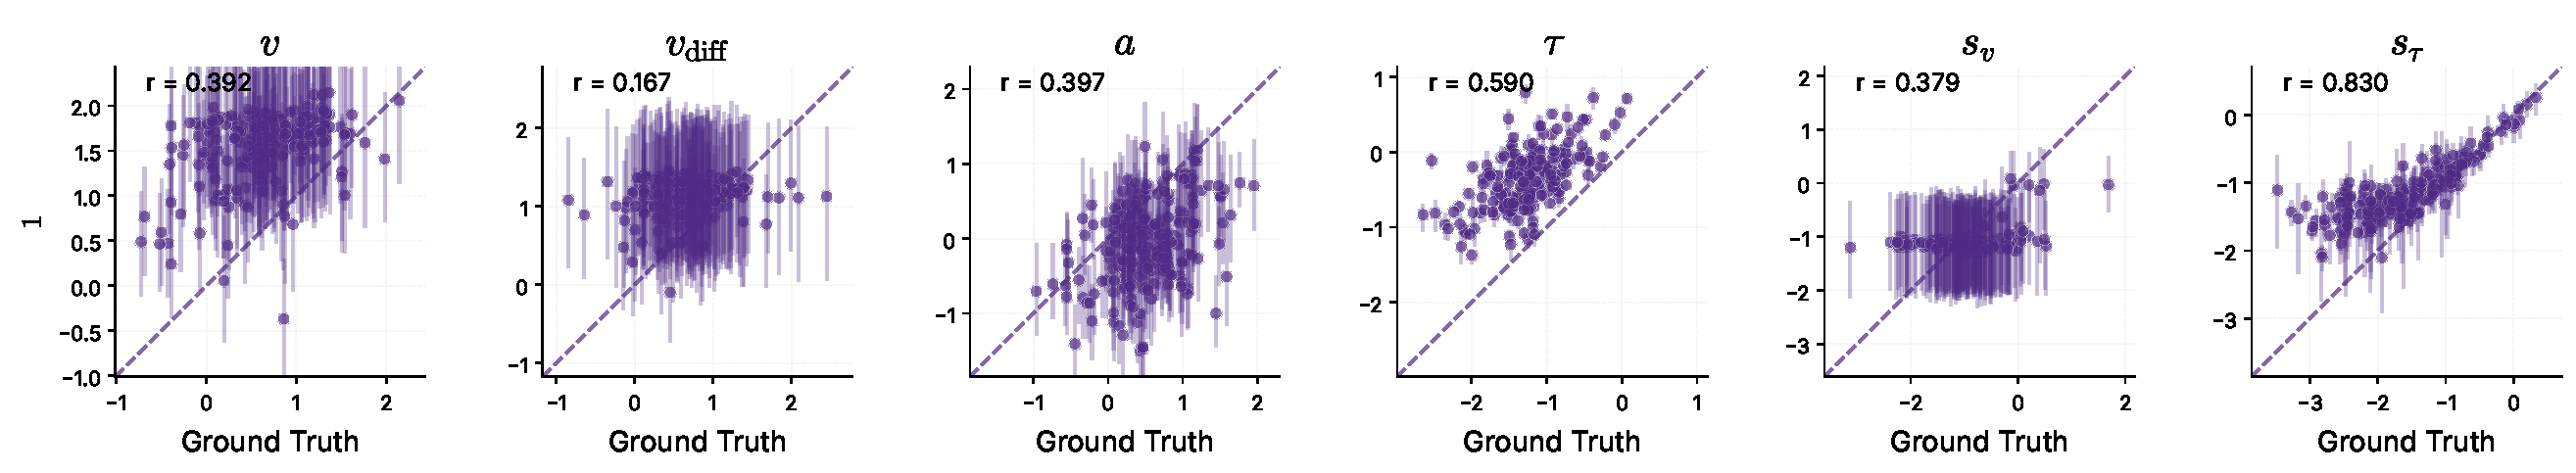
\includegraphics[width=\textwidth,height=0.3\textheight,keepaspectratio]{zeroshot/lba/intercept_only/recovery.pdf}
    \caption{Recovery}
  \end{subfigure}\\[1ex]
  \begin{subfigure}{\textwidth}\centering
    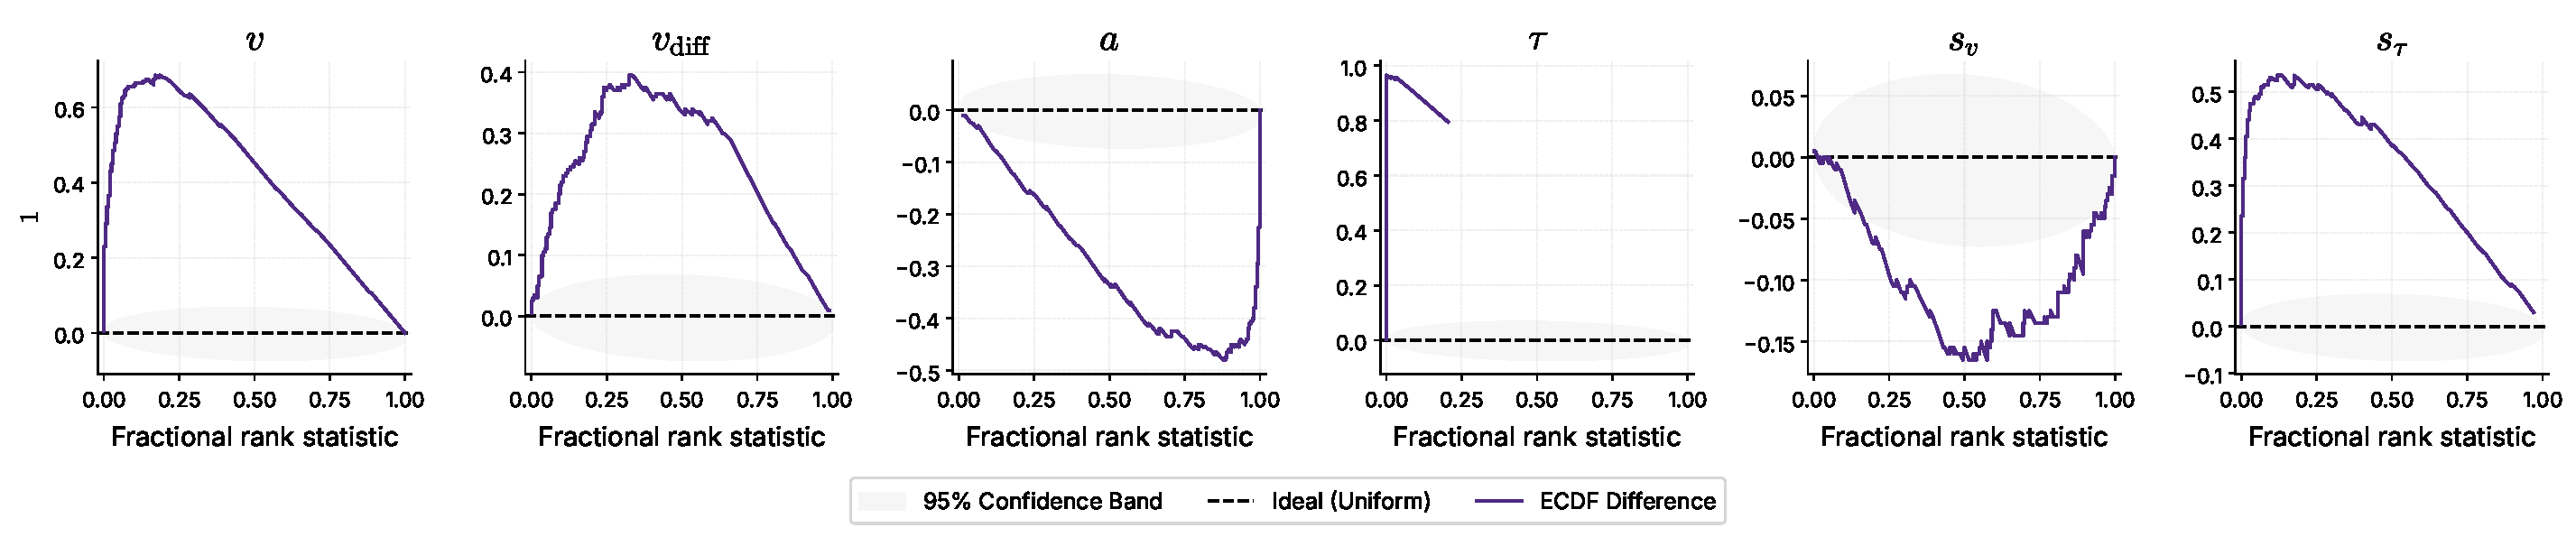
\includegraphics[width=\textwidth,height=0.3\textheight,keepaspectratio]{zeroshot/lba/intercept_only/ecdf.pdf}
    \caption{Calibration (ECDF)}
  \end{subfigure}\\[1ex]
  \begin{subfigure}{\textwidth}\centering
    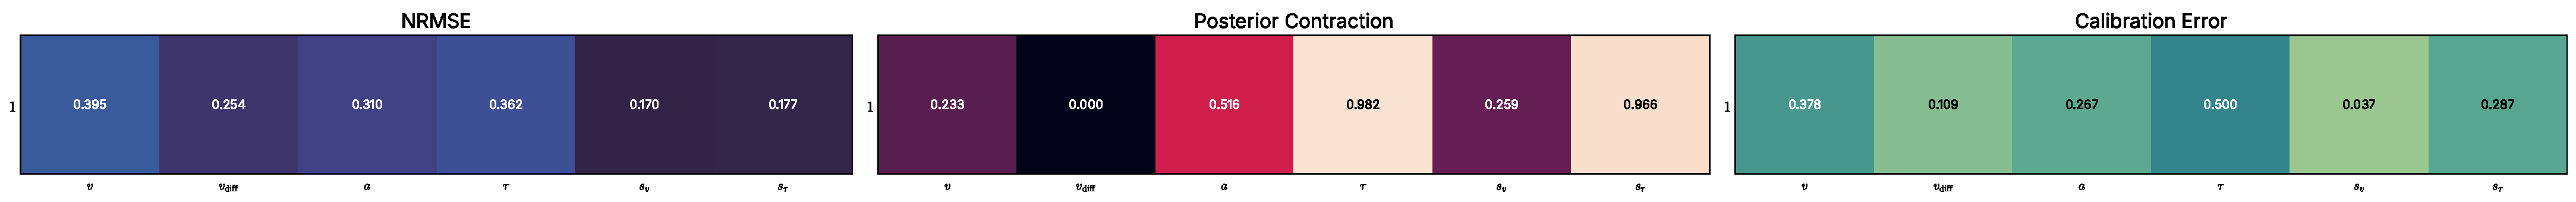
\includegraphics[width=\textwidth]{zeroshot/lba/intercept_only/metrics.pdf}
    \caption{Metrics}
  \end{subfigure}
  \caption{\textbf{Zero-shot LBA, \emph{intercept-only} design.} (a) Recovery, (b) calibration and (c) summary metrics of the original CogFormer network, trained on DDM, RDM and CDM only, applied to the held-out LBA without any LBA training. The network is run under the RDM's model embedding, whose parameters ($v$, $v_{\mathrm{diff}}$, $a$, $\tau$, $s_v$, $s_\tau$, $\pi$) the LBA shares; the LBA's start-point range is fixed at $A = 0.5$, and $a$ is the mean distance an accumulator travels to its threshold, the quantity the RDM's $a$ measures. Evaluated on the 200 bench5 LBA test datasets (500 trials each, two stimulus-coded alternatives), with 200 posterior draws per dataset; panels encoded as in Figure~\ref{fig:app1-ddm-intercept-only-cf}. Every estimated parameter enters as an intercept only (6 coefficients shown). All subsequent zero-shot figures (Figures~\ref{fig:app3-zeroshot-lba-fixed}--\ref{fig:app3-zeroshot-lba-mixed-predictor-metrics}) follow this layout; the mixed-predictor design, whose grids are long, is shown as three separate figures.}
  \label{fig:app3-zeroshot-lba-intercept-only}
\end{figure}

\begin{figure}[p]
  \centering
  \begin{subfigure}{\textwidth}\centering
    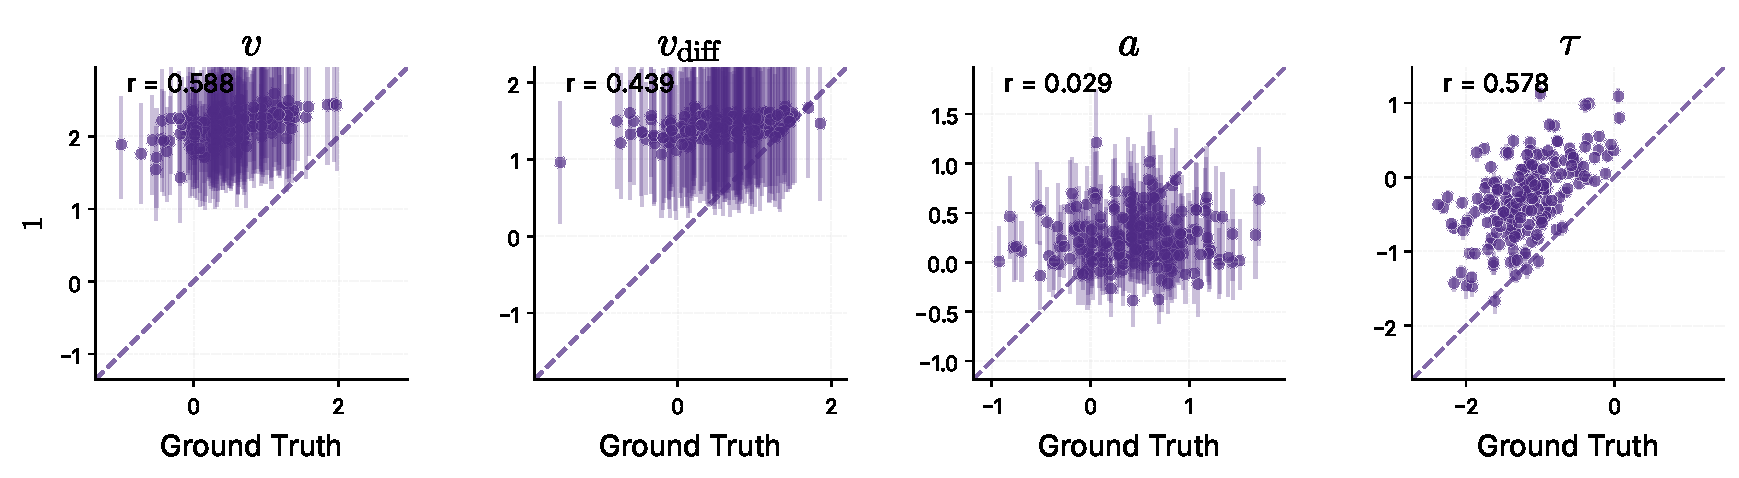
\includegraphics[width=\textwidth,height=0.3\textheight,keepaspectratio]{zeroshot/lba/fixed/recovery.pdf}
    \caption{Recovery}
  \end{subfigure}\\[1ex]
  \begin{subfigure}{\textwidth}\centering
    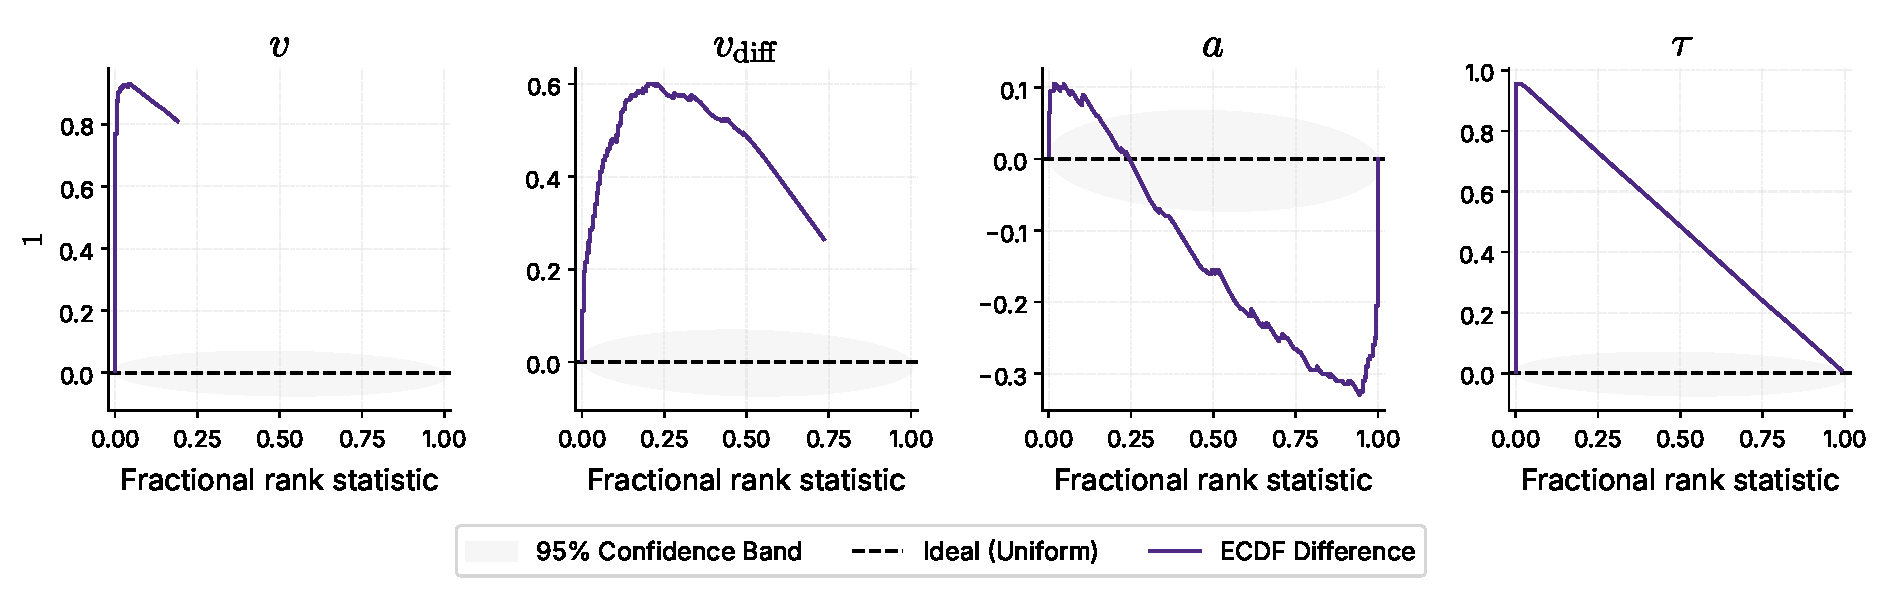
\includegraphics[width=\textwidth,height=0.3\textheight,keepaspectratio]{zeroshot/lba/fixed/ecdf.pdf}
    \caption{Calibration (ECDF)}
  \end{subfigure}\\[1ex]
  \begin{subfigure}{\textwidth}\centering
    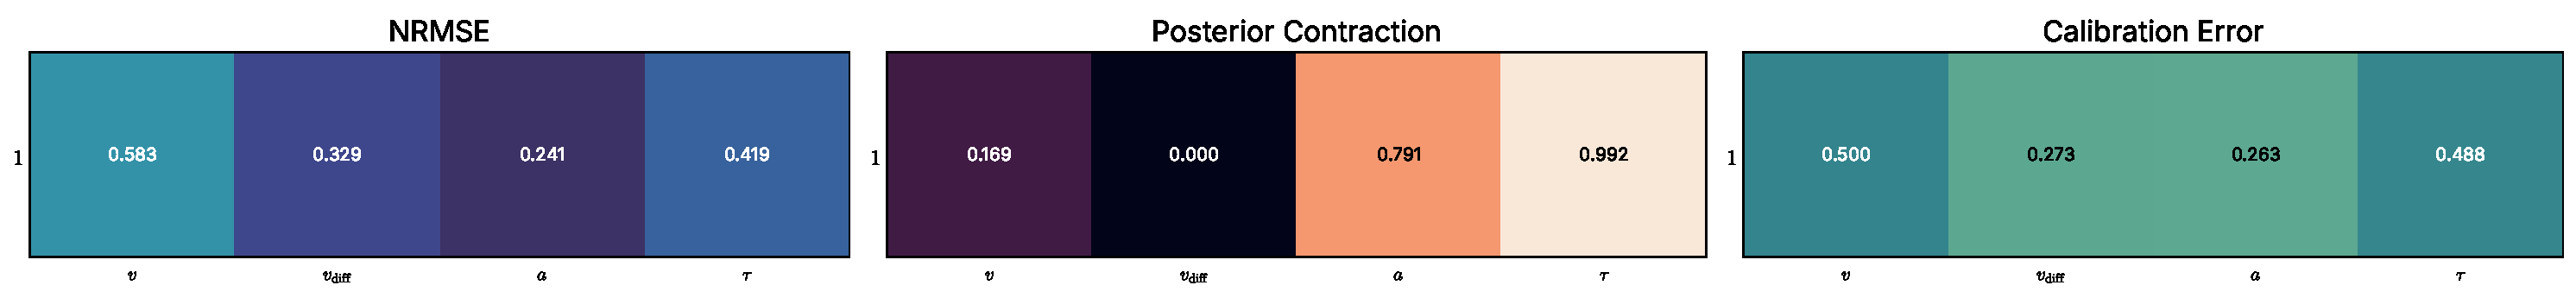
\includegraphics[width=\textwidth]{zeroshot/lba/fixed/metrics.pdf}
    \caption{Metrics}
  \end{subfigure}
  \caption{\textbf{Zero-shot LBA, \emph{fixed} design.} (a) Recovery, (b) calibration, (c) metrics. $s_v$ and $s_\tau$ are fixed at 0 and not estimated; every estimated parameter enters as an intercept only (4 coefficients shown). As in Figure~\ref{fig:app3-zeroshot-lba-intercept-only}.}
  \label{fig:app3-zeroshot-lba-fixed}
\end{figure}

\begin{figure}[p]
  \centering
  \begin{subfigure}{\textwidth}\centering
    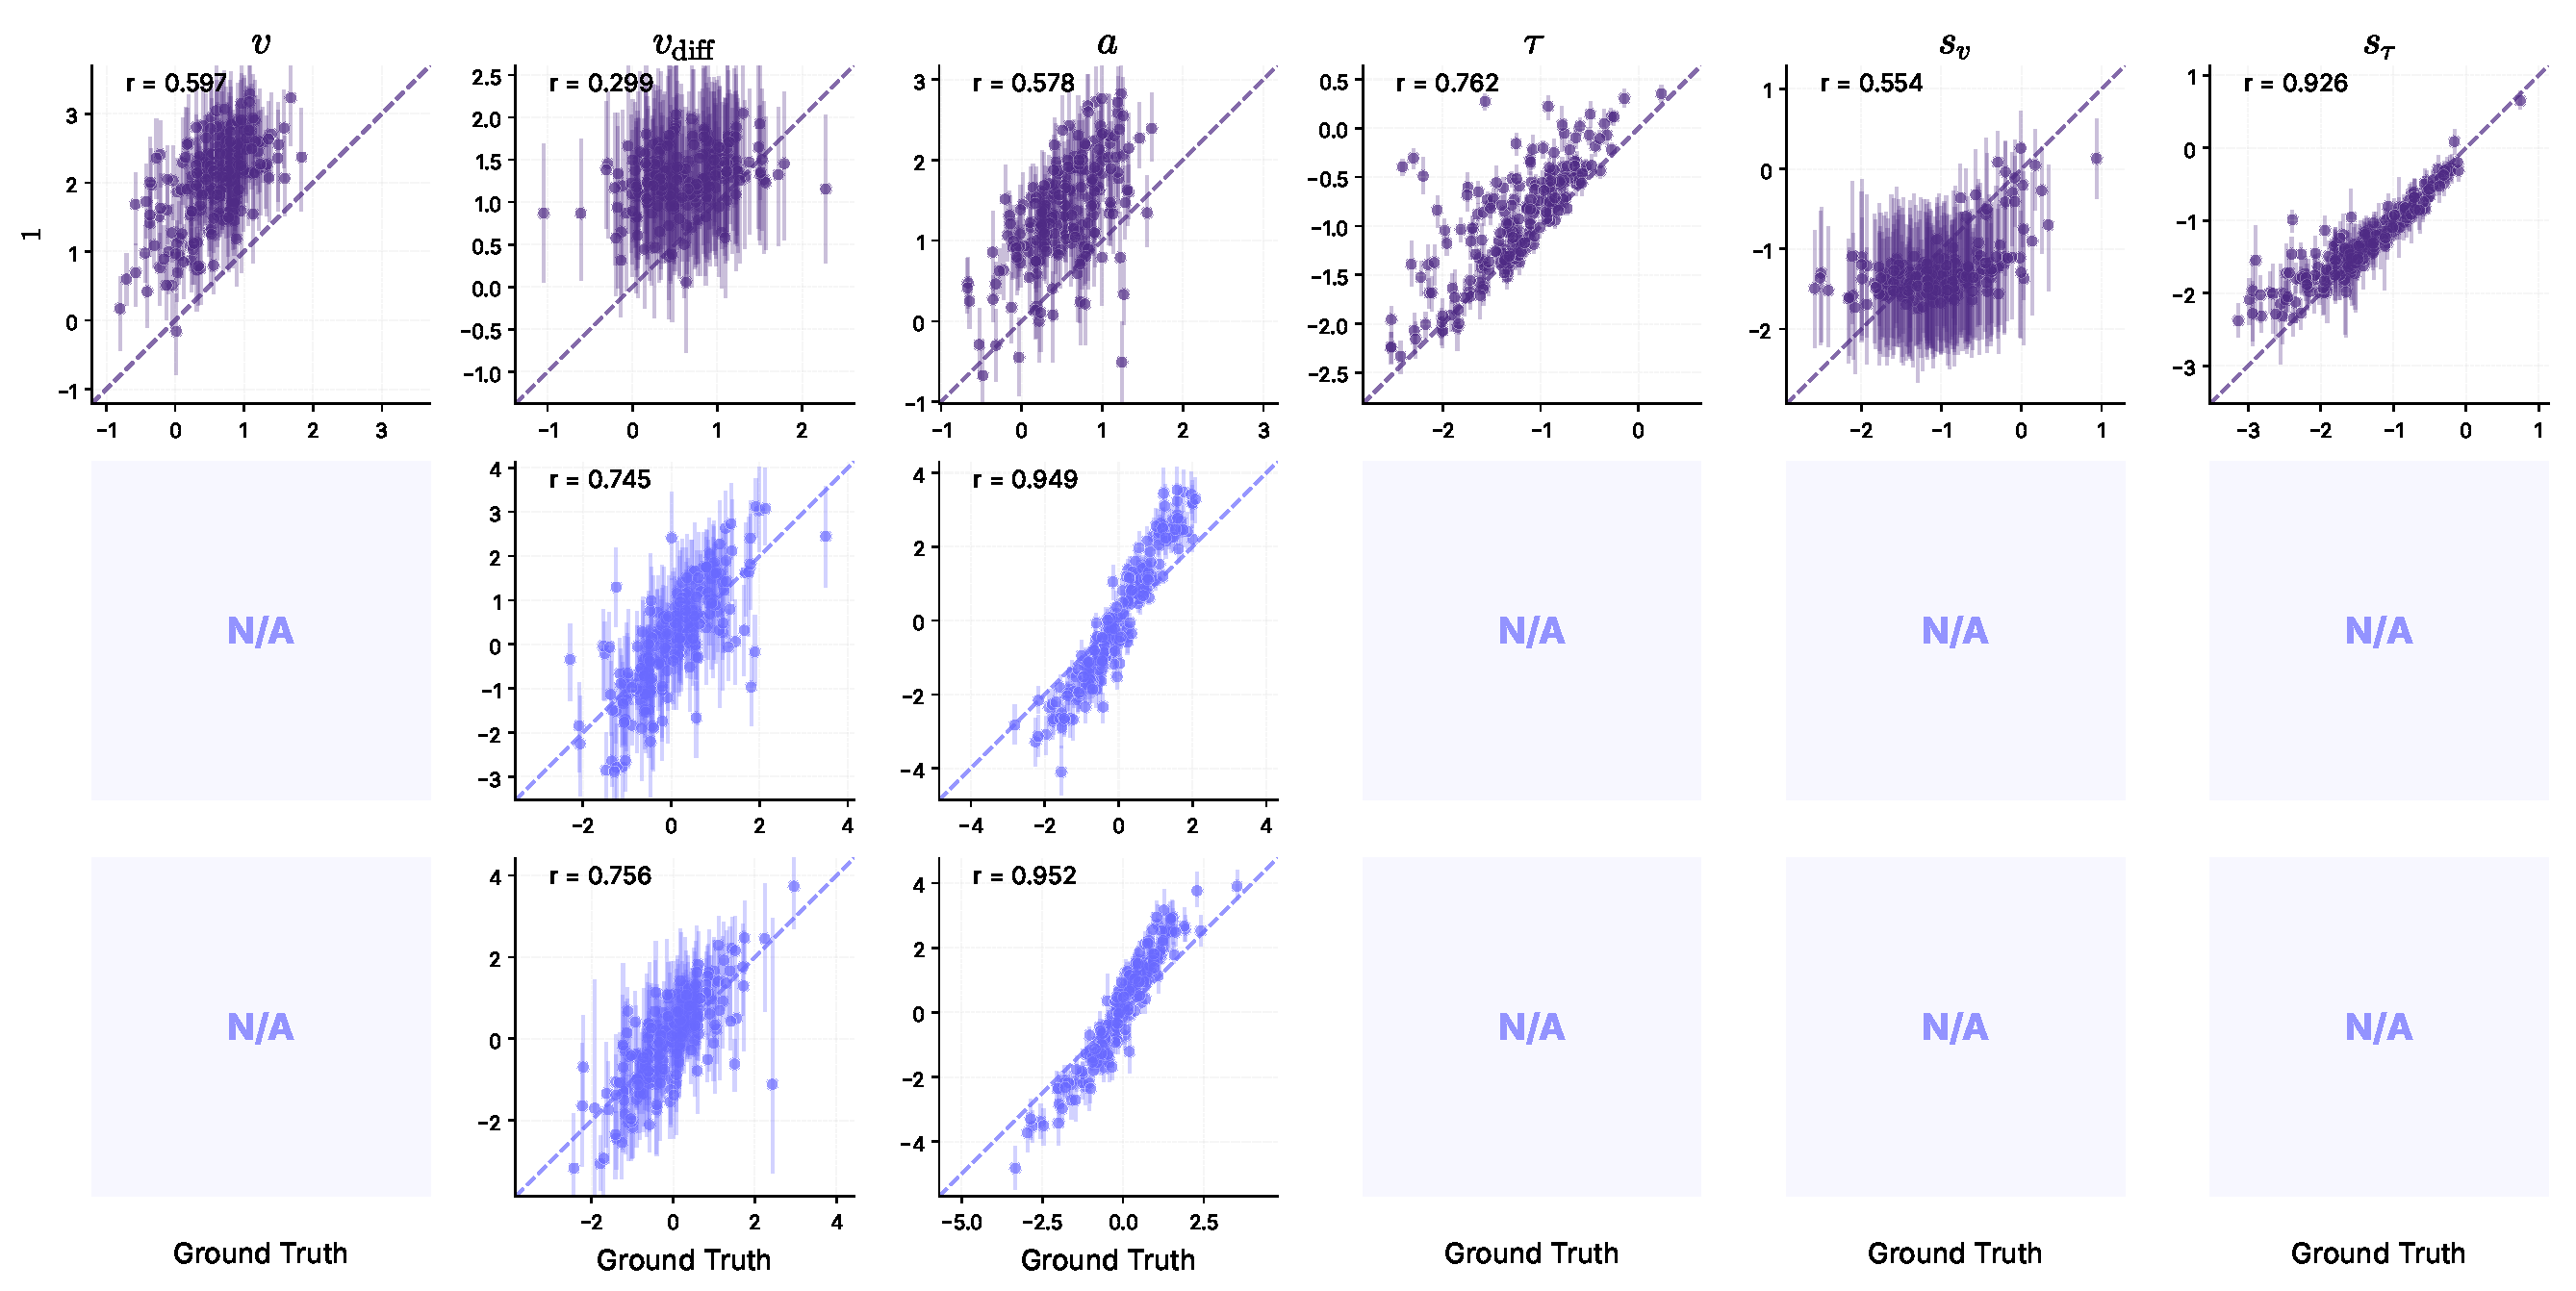
\includegraphics[width=\textwidth,height=0.3\textheight,keepaspectratio]{zeroshot/lba/regressed/recovery.pdf}
    \caption{Recovery}
  \end{subfigure}\\[1ex]
  \begin{subfigure}{\textwidth}\centering
    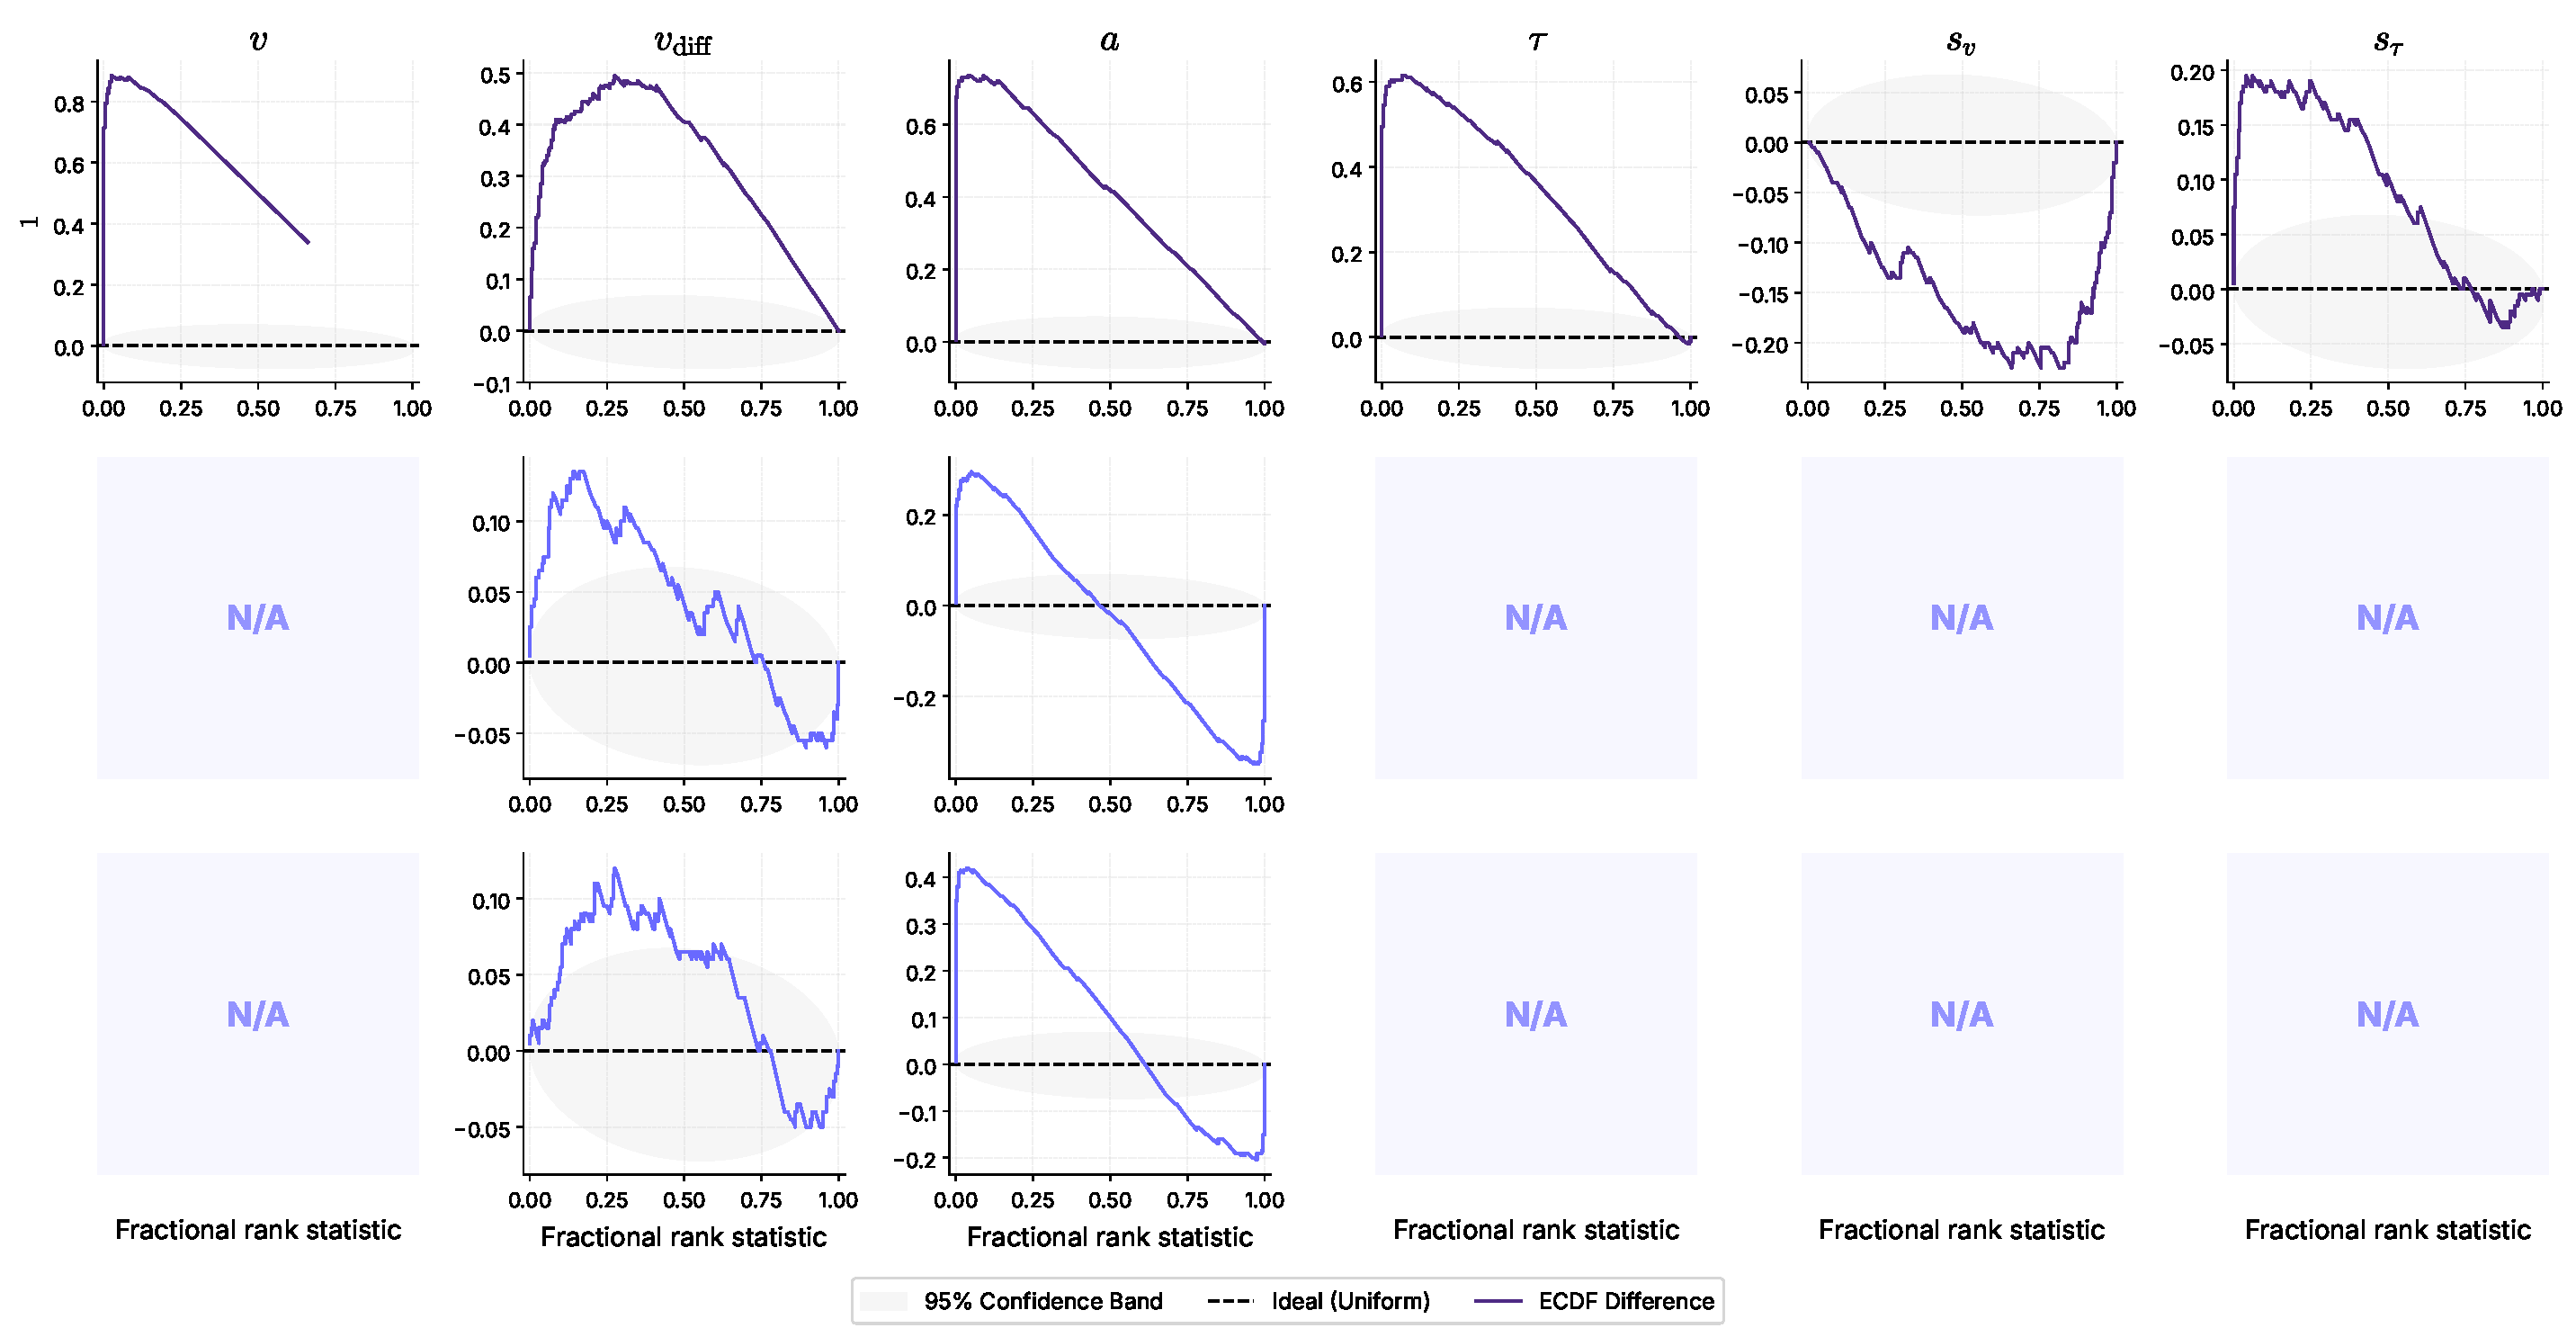
\includegraphics[width=\textwidth,height=0.3\textheight,keepaspectratio]{zeroshot/lba/regressed/ecdf.pdf}
    \caption{Calibration (ECDF)}
  \end{subfigure}\\[1ex]
  \begin{subfigure}{\textwidth}\centering
    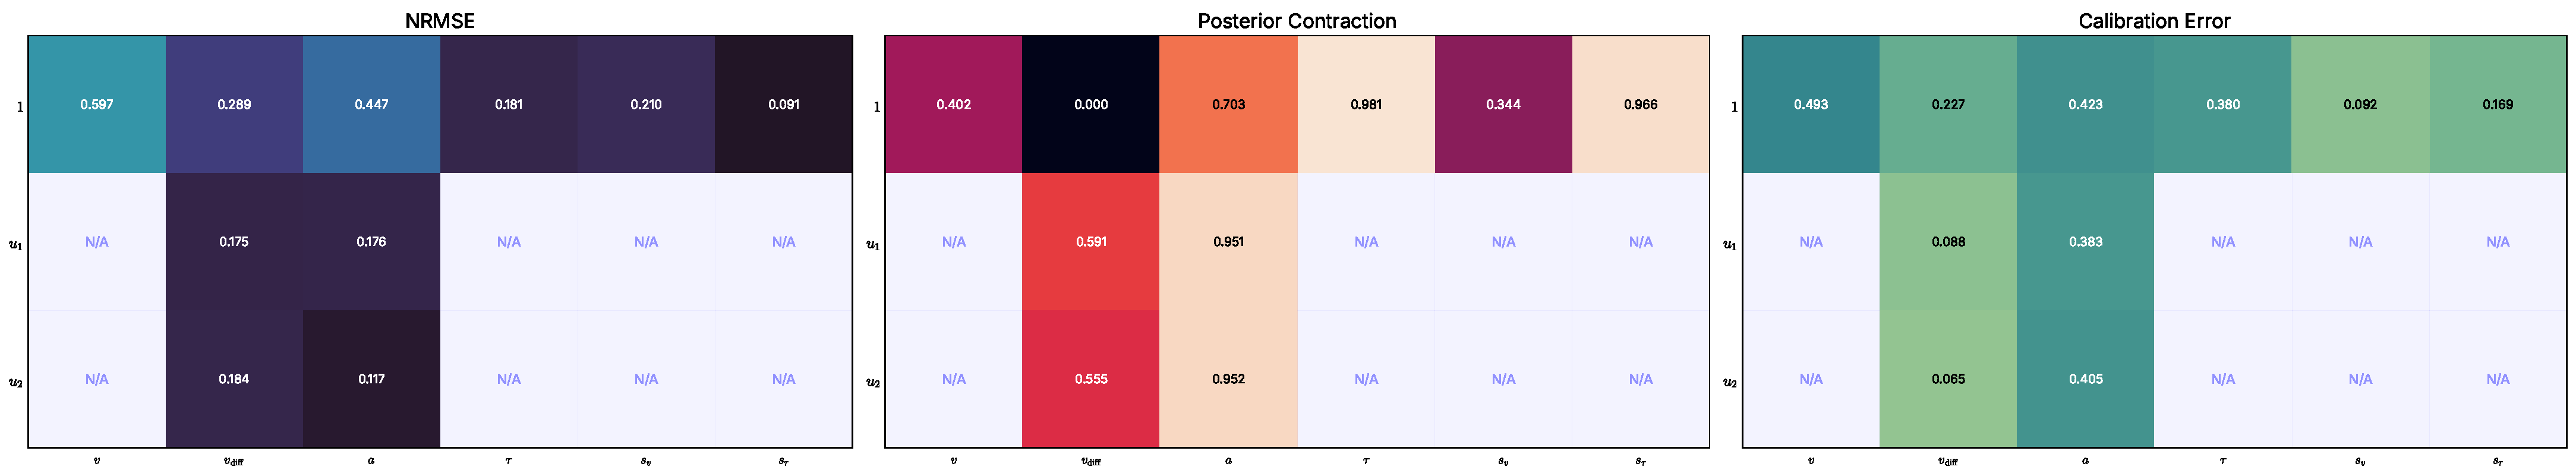
\includegraphics[width=\textwidth]{zeroshot/lba/regressed/metrics.pdf}
    \caption{Metrics}
  \end{subfigure}
  \caption{\textbf{Zero-shot LBA, \emph{regressed} design.} (a) Recovery, (b) calibration, (c) metrics. $v_{\mathrm{diff}}$ and $a$ carry slopes on $u_1$ and $u_2$ (10 coefficients shown). As in Figure~\ref{fig:app3-zeroshot-lba-intercept-only}.}
  \label{fig:app3-zeroshot-lba-regressed}
\end{figure}

\begin{figure}[p]
  \centering
  \begin{subfigure}{\textwidth}\centering
    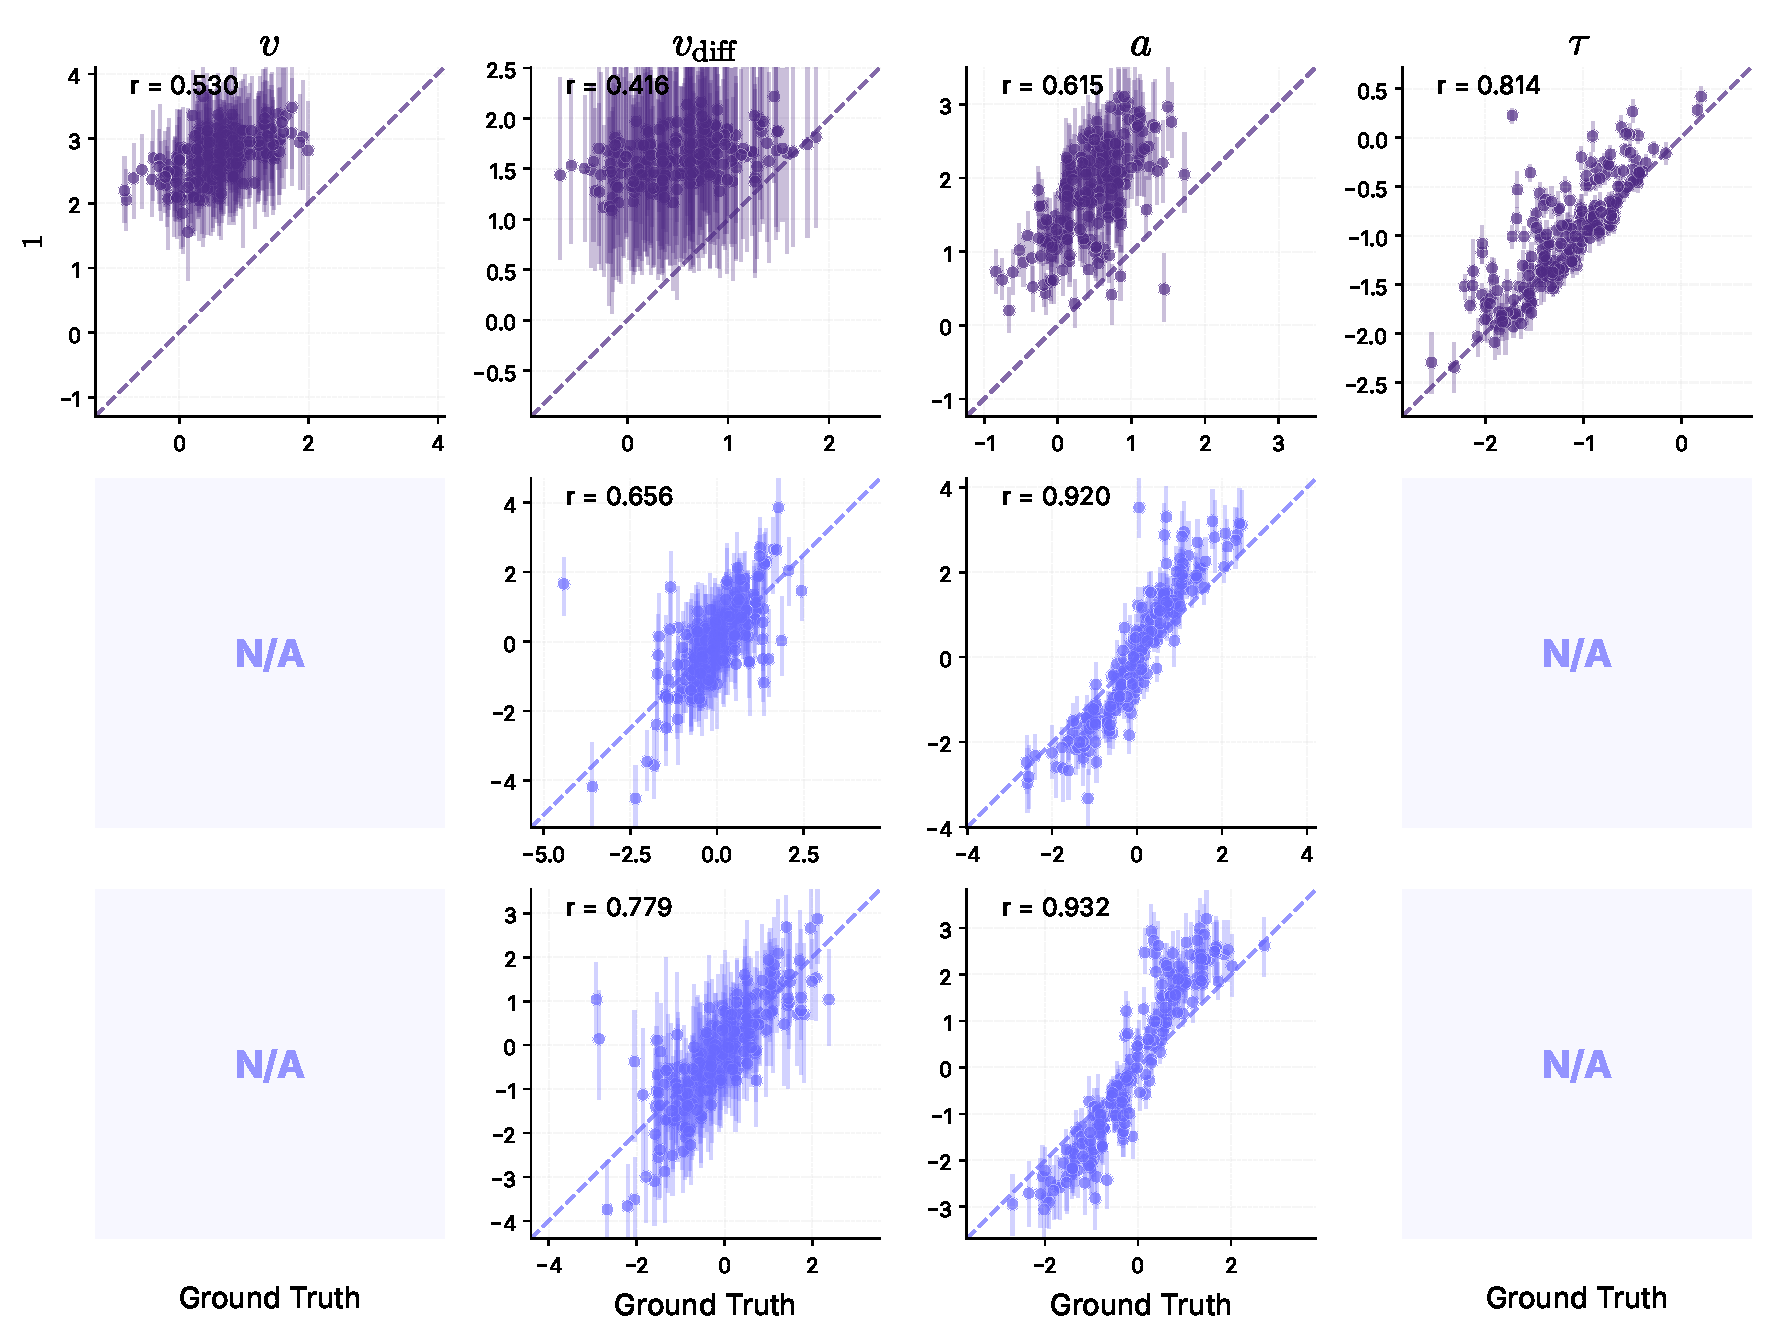
\includegraphics[width=\textwidth,height=0.3\textheight,keepaspectratio]{zeroshot/lba/fixed_regressed/recovery.pdf}
    \caption{Recovery}
  \end{subfigure}\\[1ex]
  \begin{subfigure}{\textwidth}\centering
    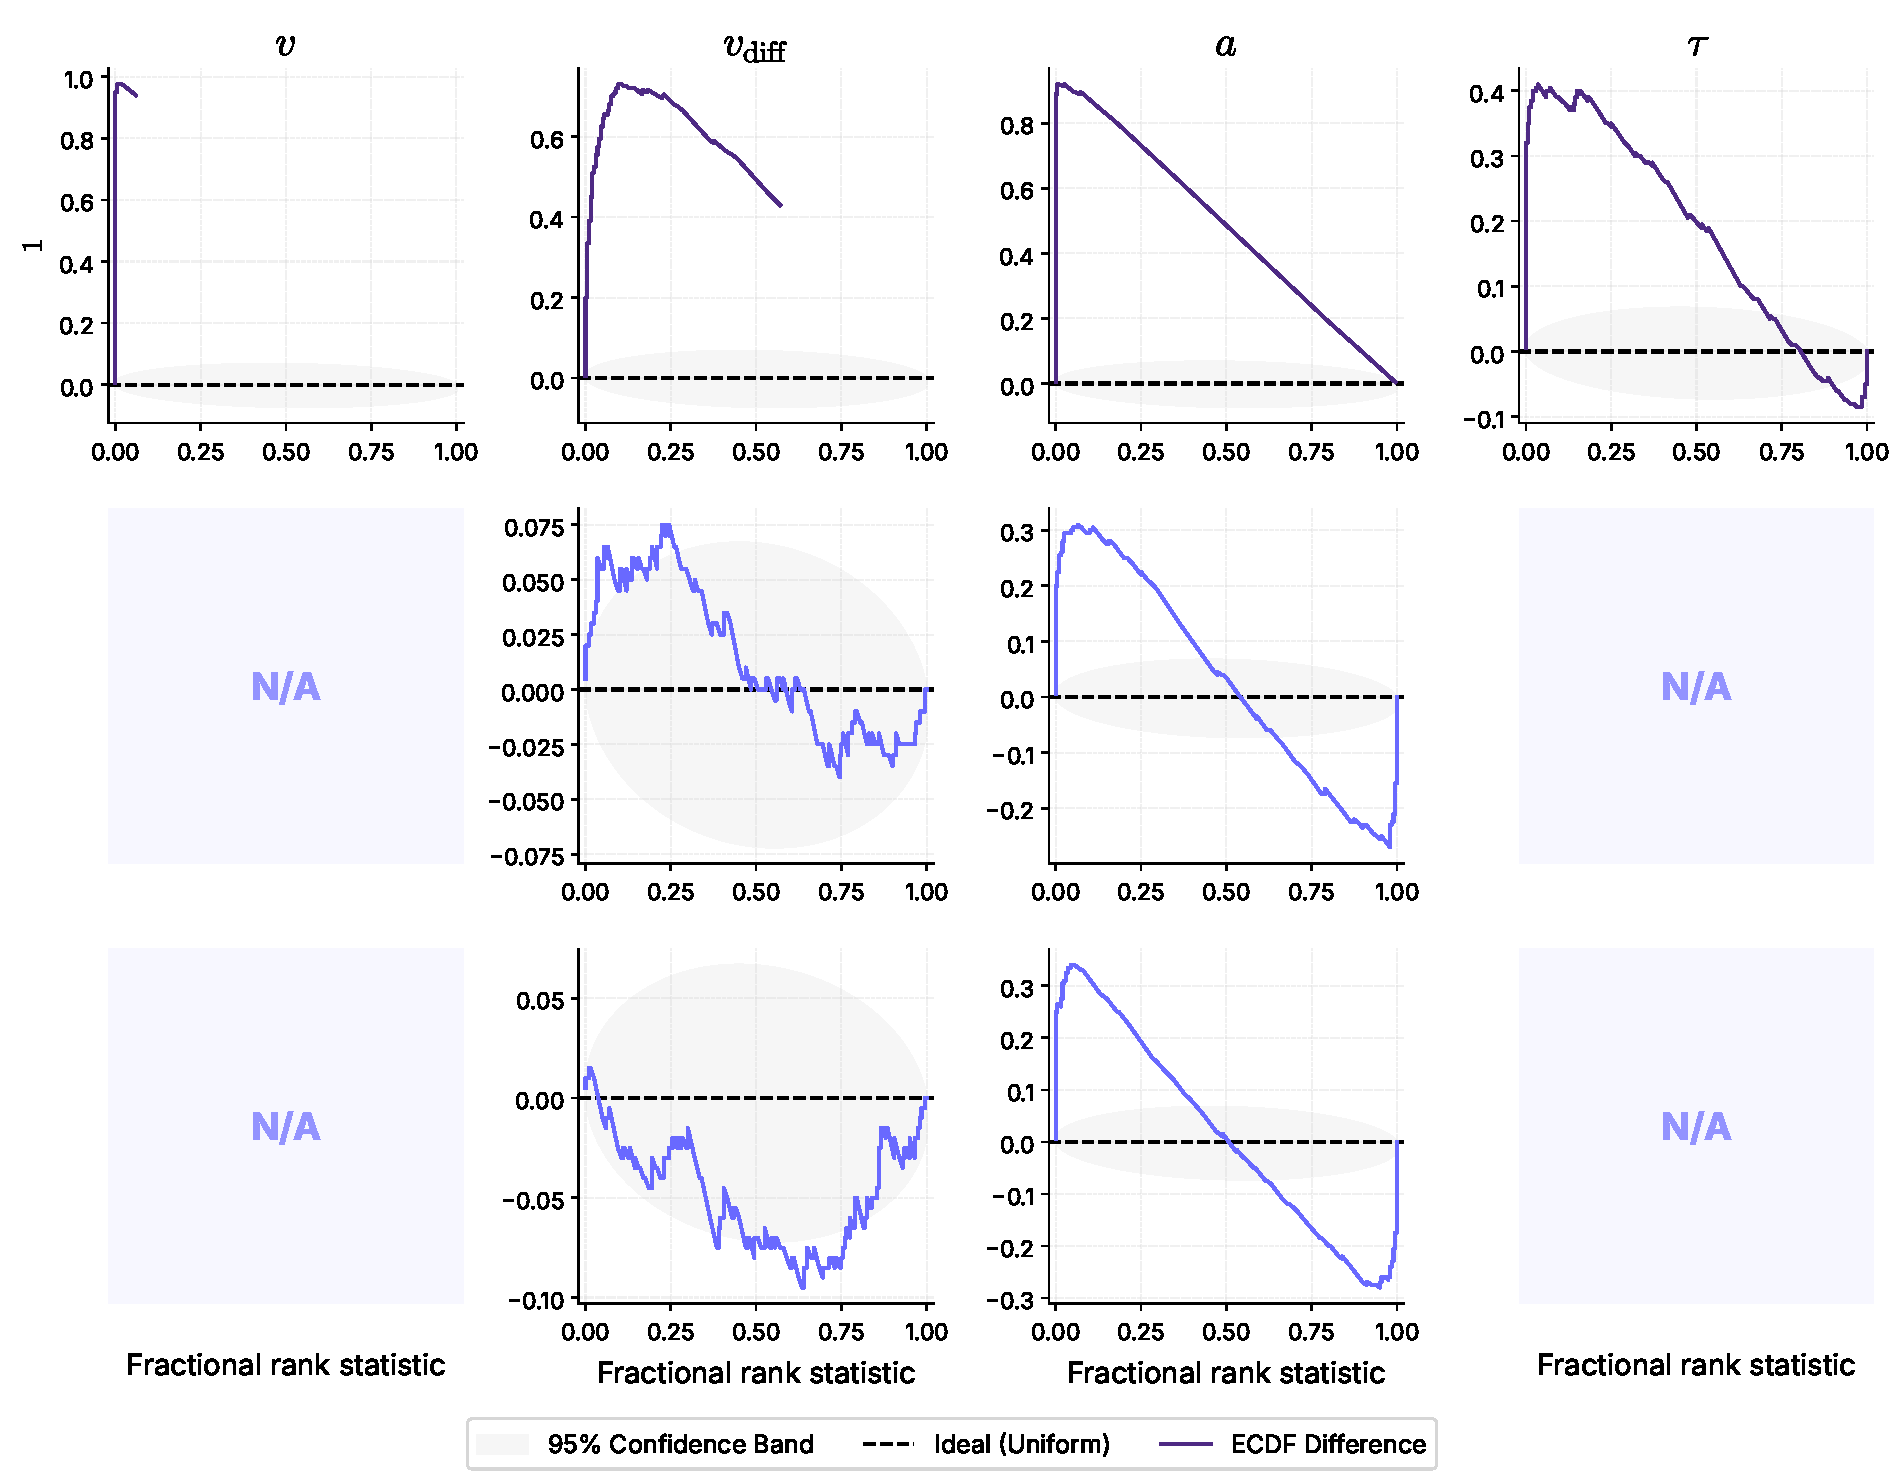
\includegraphics[width=\textwidth,height=0.3\textheight,keepaspectratio]{zeroshot/lba/fixed_regressed/ecdf.pdf}
    \caption{Calibration (ECDF)}
  \end{subfigure}\\[1ex]
  \begin{subfigure}{\textwidth}\centering
    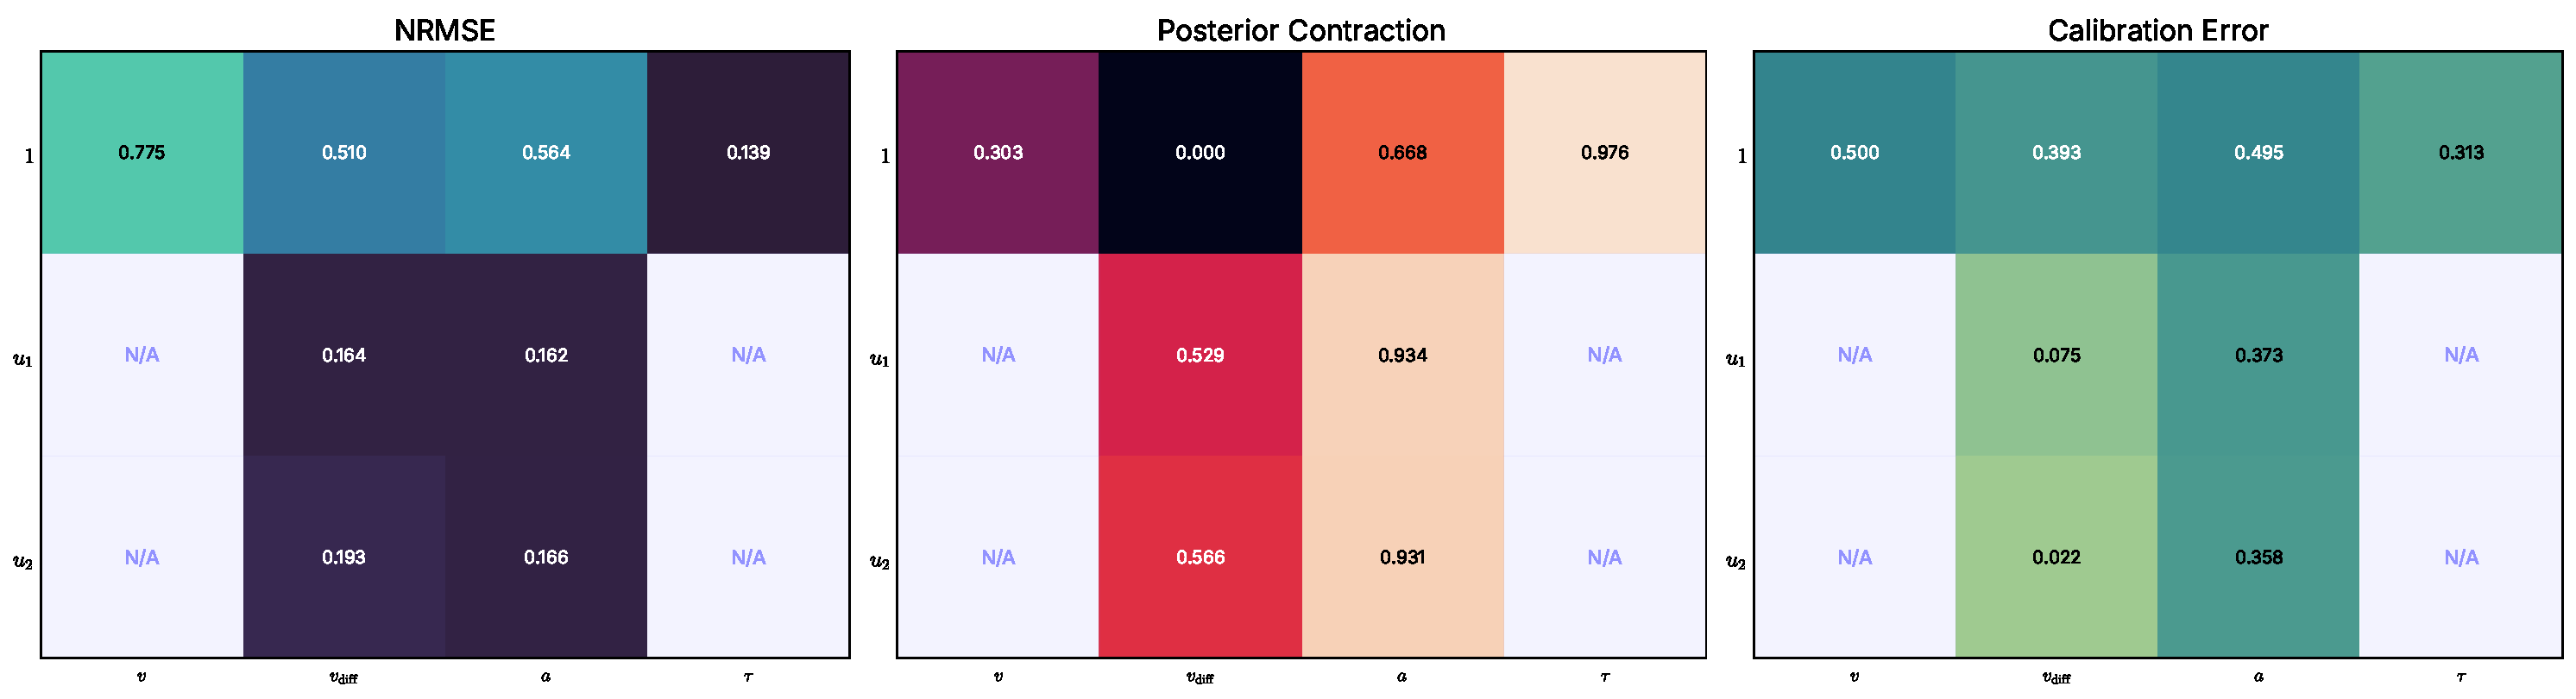
\includegraphics[width=\textwidth]{zeroshot/lba/fixed_regressed/metrics.pdf}
    \caption{Metrics}
  \end{subfigure}
  \caption{\textbf{Zero-shot LBA, \emph{fixed + regressed} design.} (a) Recovery, (b) calibration, (c) metrics. $s_v$ and $s_\tau$ are fixed at 0 and not estimated; $v_{\mathrm{diff}}$ and $a$ carry slopes on $u_1$ and $u_2$ (8 coefficients shown). As in Figure~\ref{fig:app3-zeroshot-lba-intercept-only}.}
  \label{fig:app3-zeroshot-lba-fixed-regressed}
\end{figure}

\begin{figure}[p]
  \centering
  \begin{subfigure}{\textwidth}\centering
    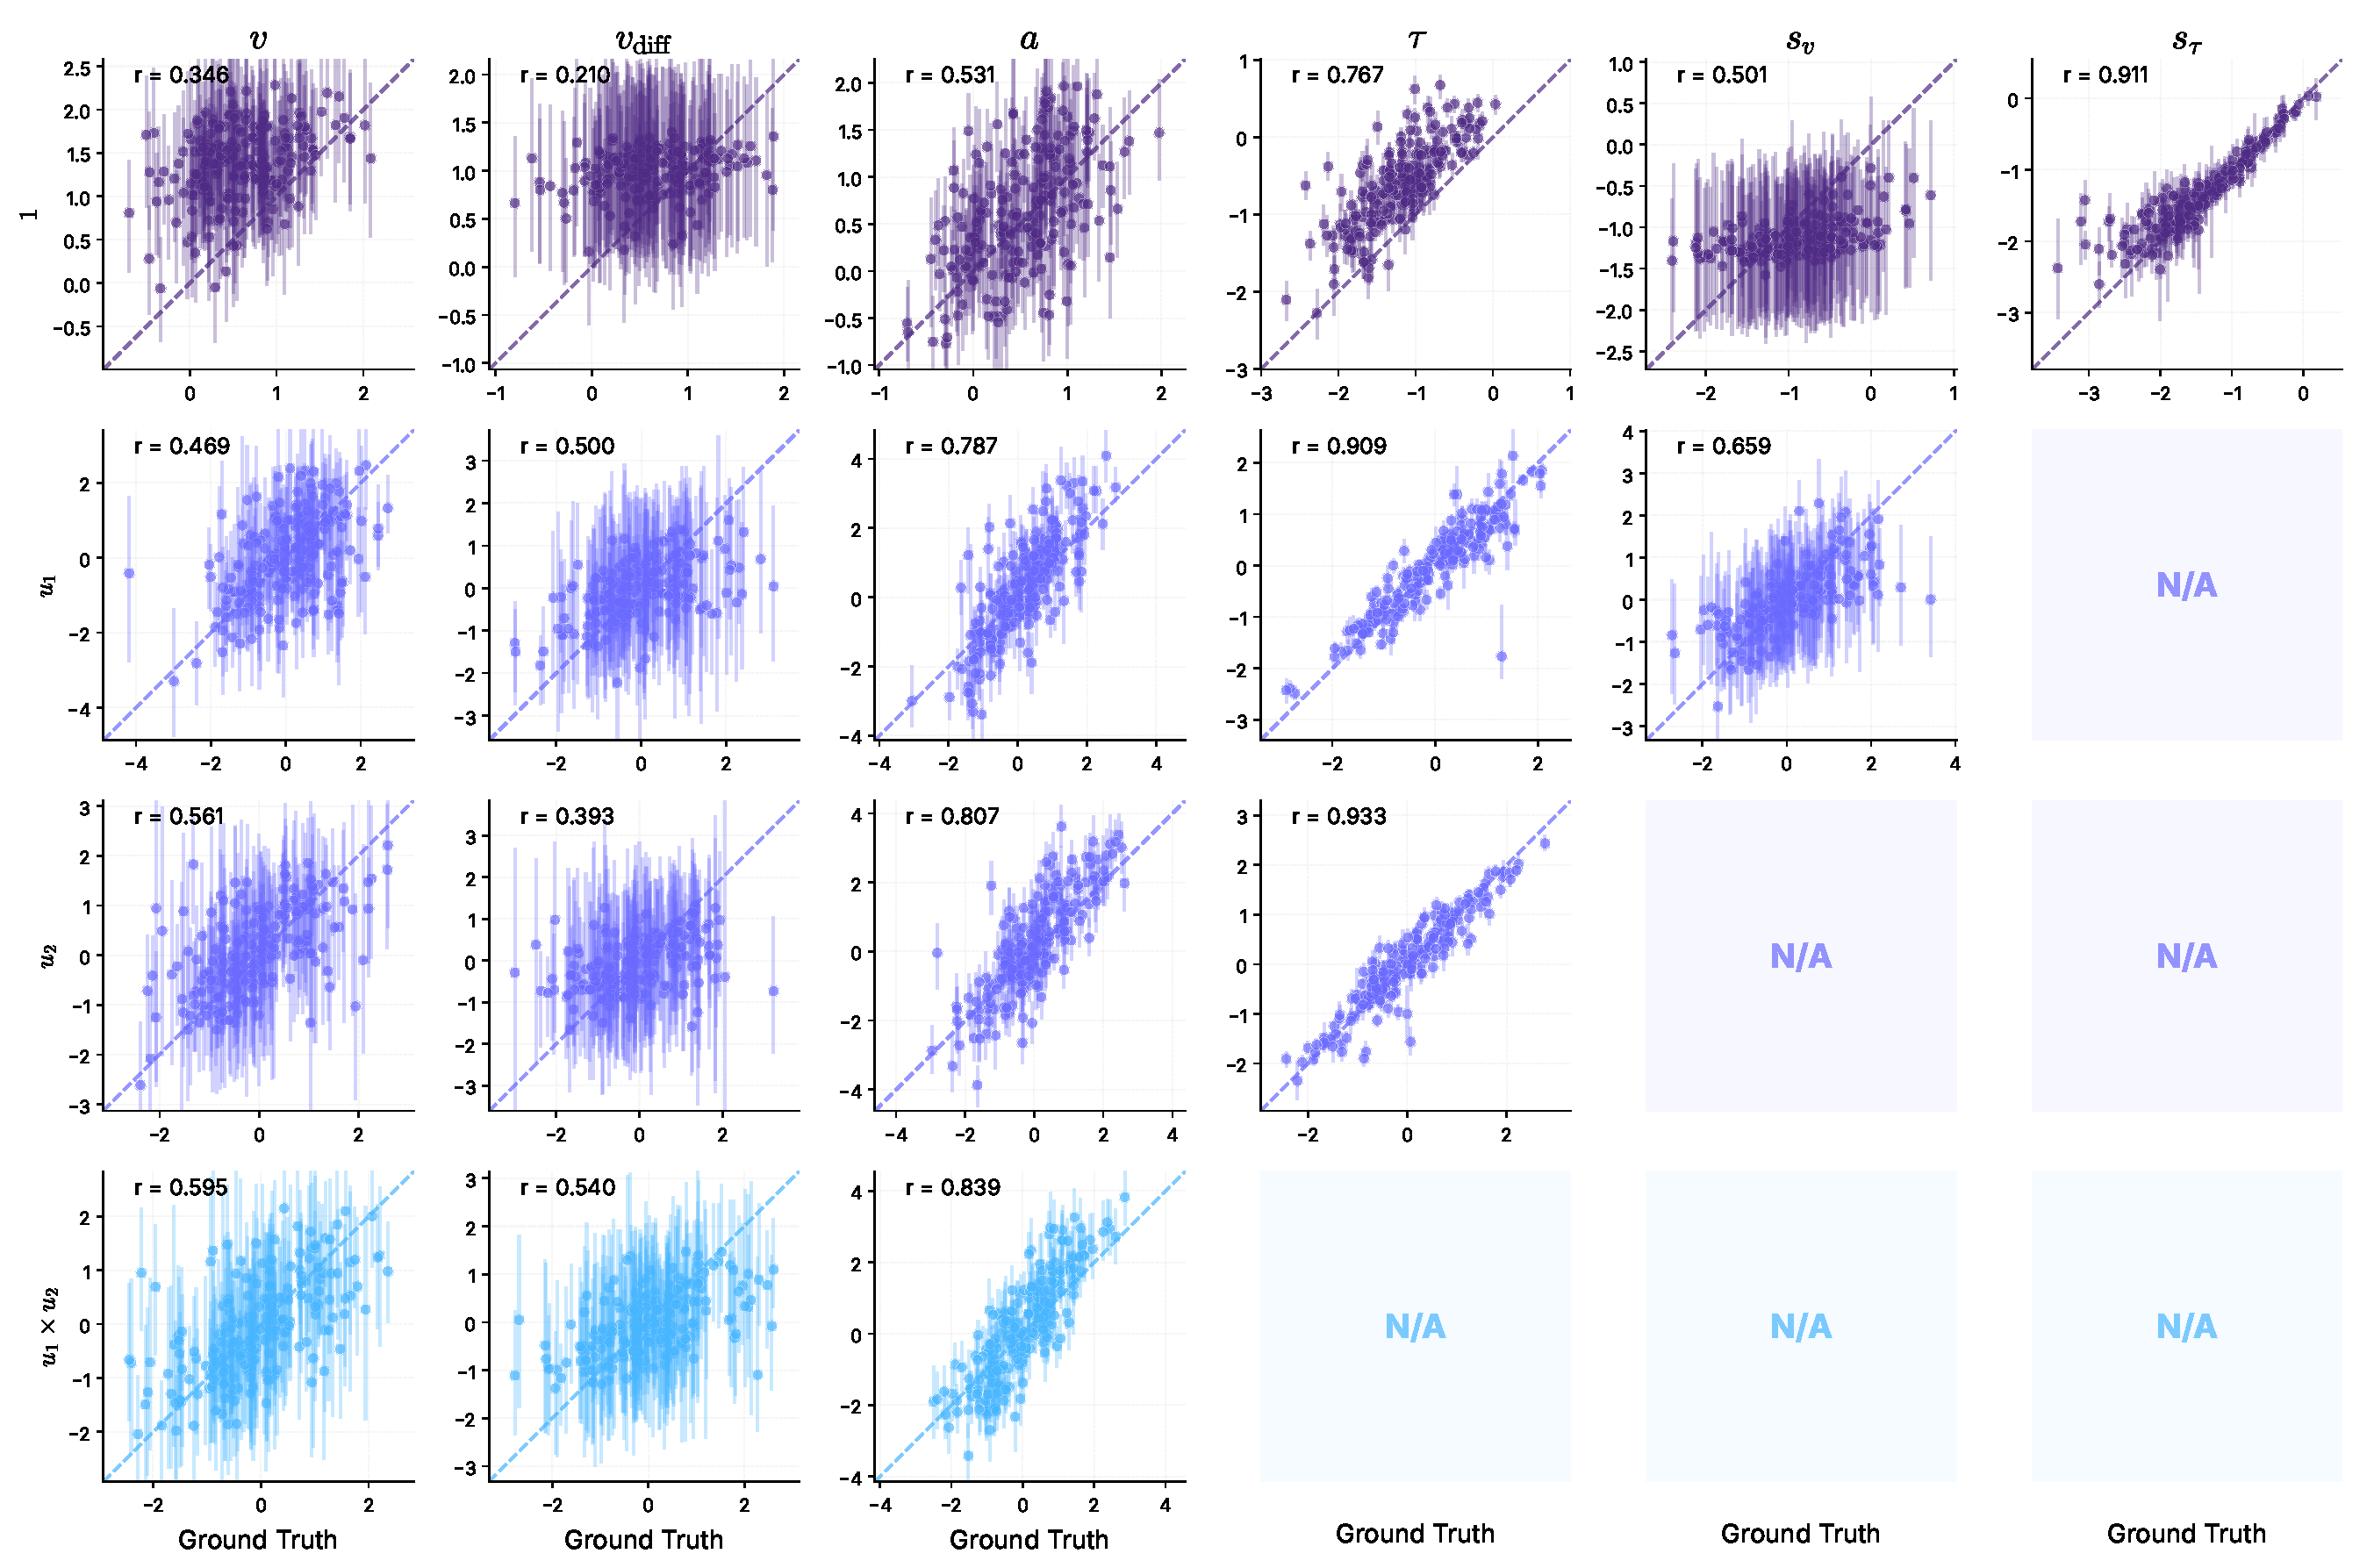
\includegraphics[width=\textwidth,height=0.3\textheight,keepaspectratio]{zeroshot/lba/interaction/recovery.pdf}
    \caption{Recovery}
  \end{subfigure}\\[1ex]
  \begin{subfigure}{\textwidth}\centering
    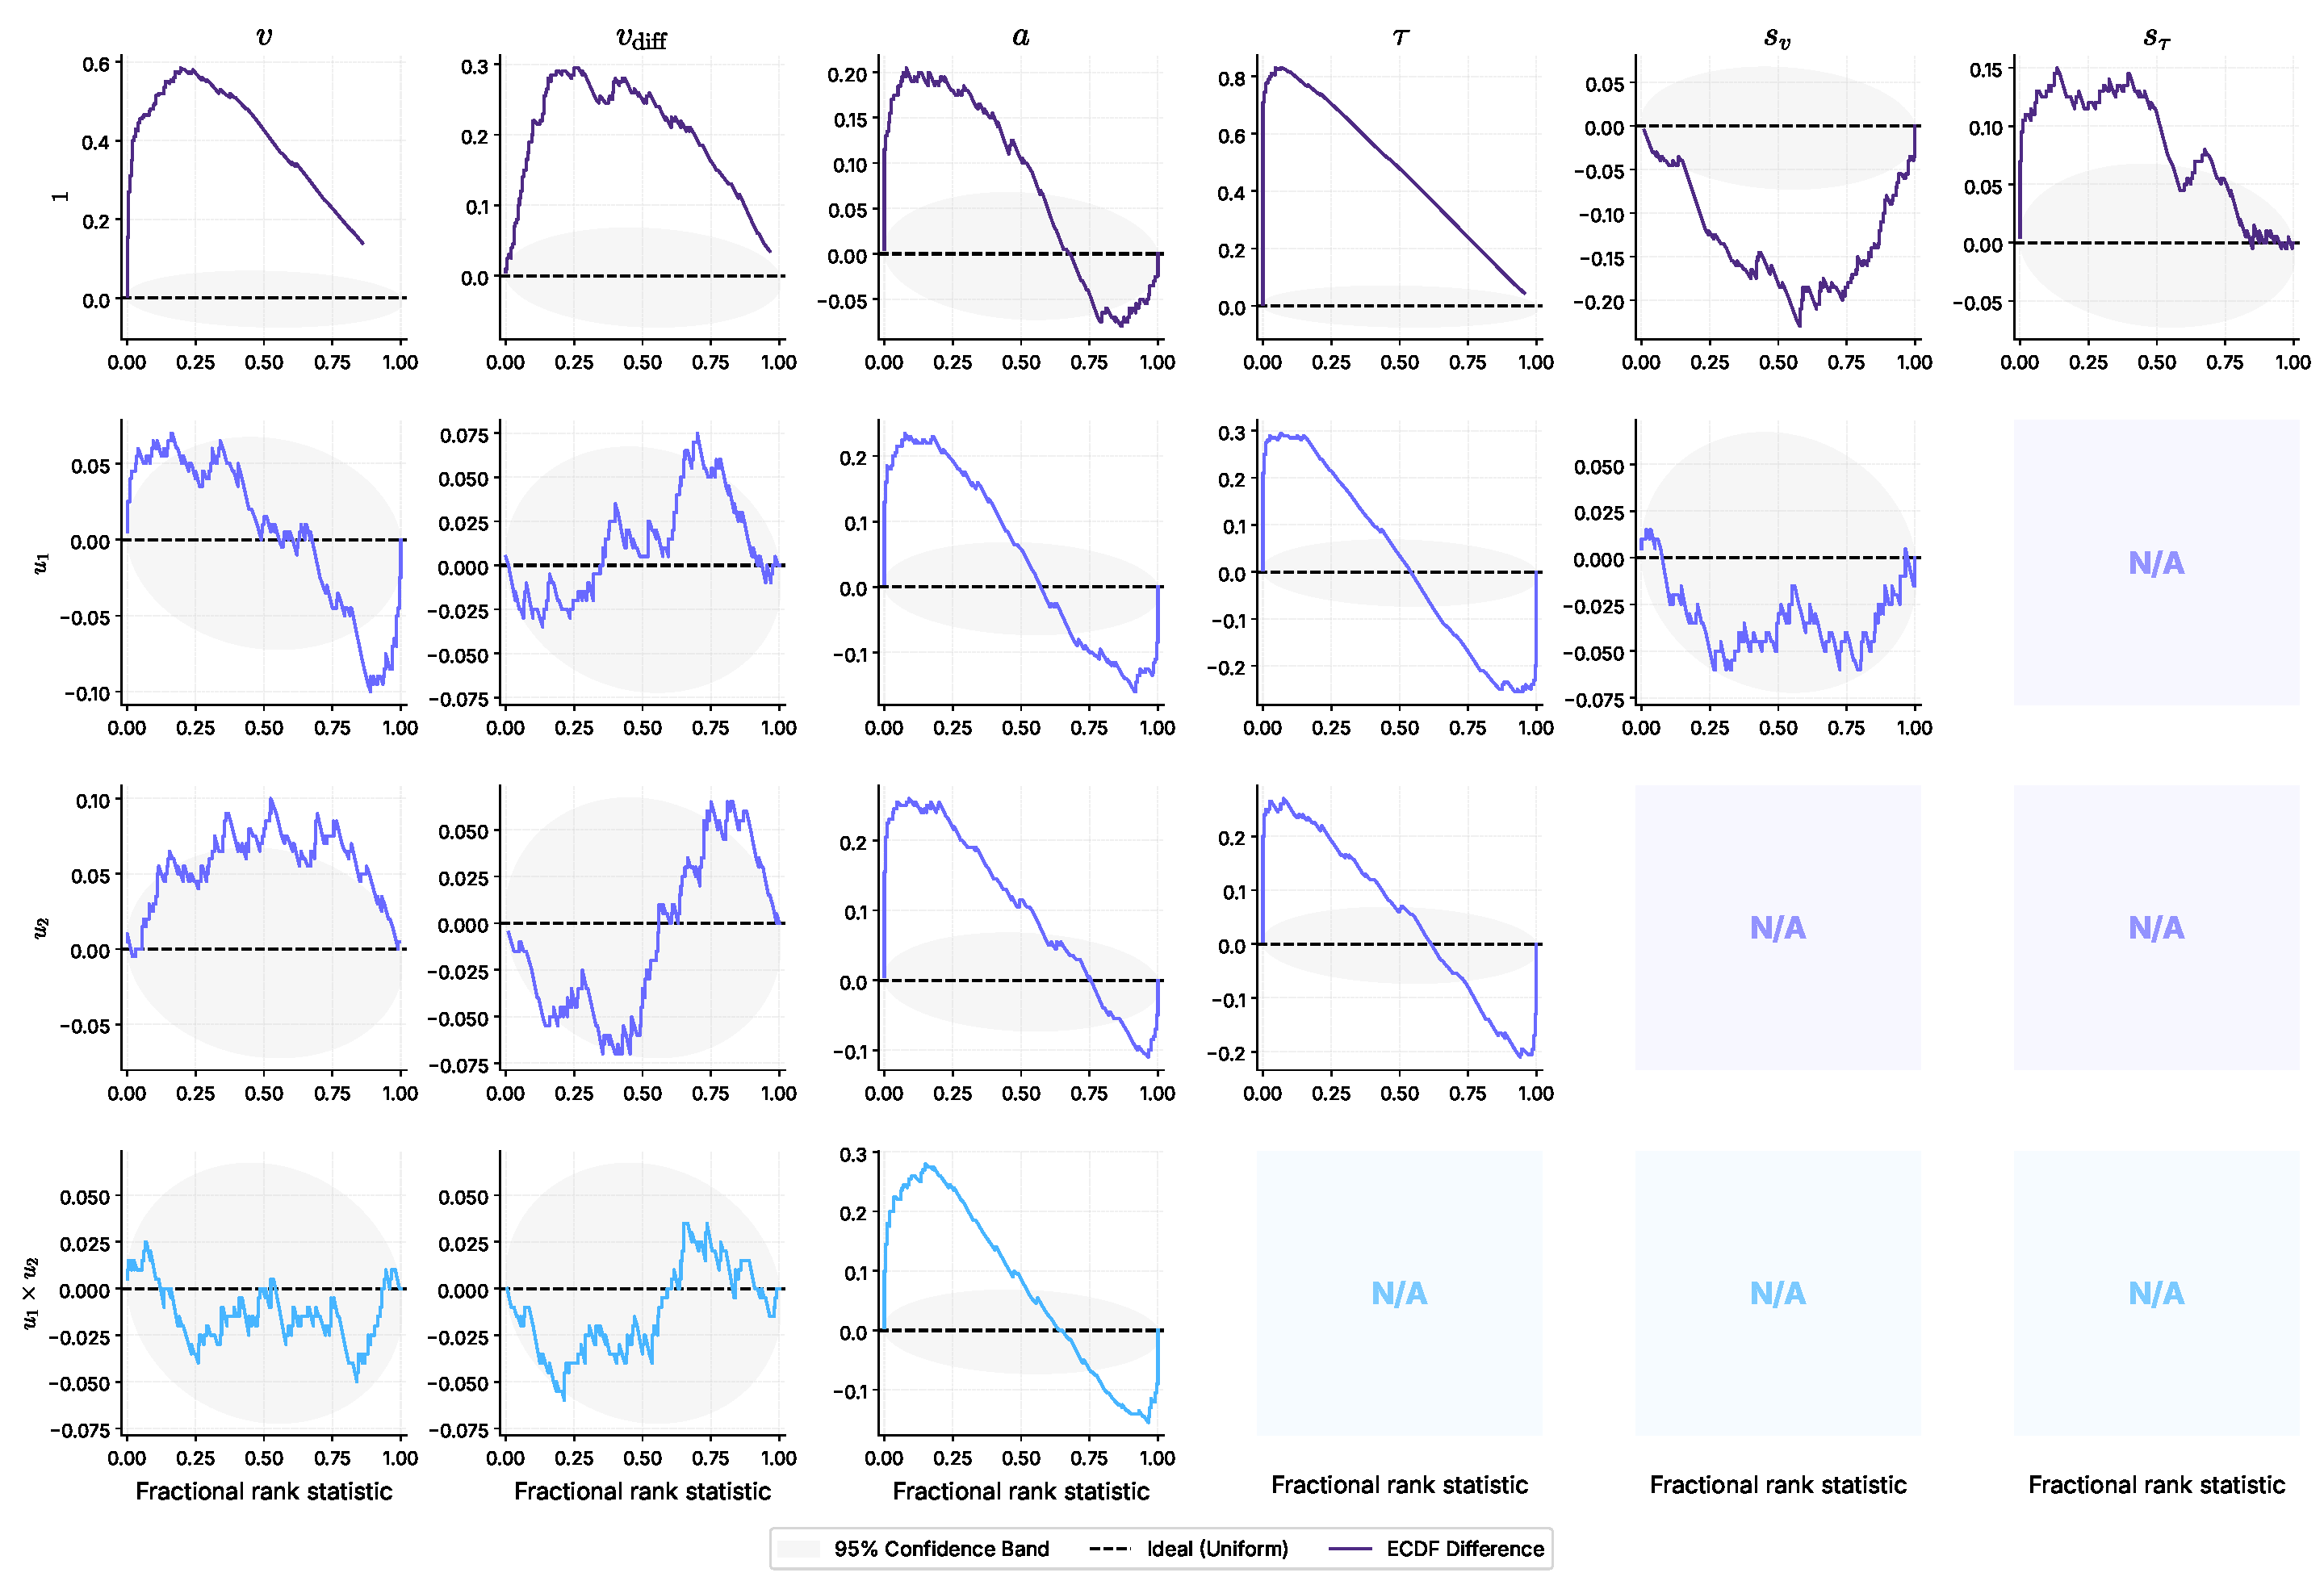
\includegraphics[width=\textwidth,height=0.3\textheight,keepaspectratio]{zeroshot/lba/interaction/ecdf.pdf}
    \caption{Calibration (ECDF)}
  \end{subfigure}\\[1ex]
  \begin{subfigure}{\textwidth}\centering
    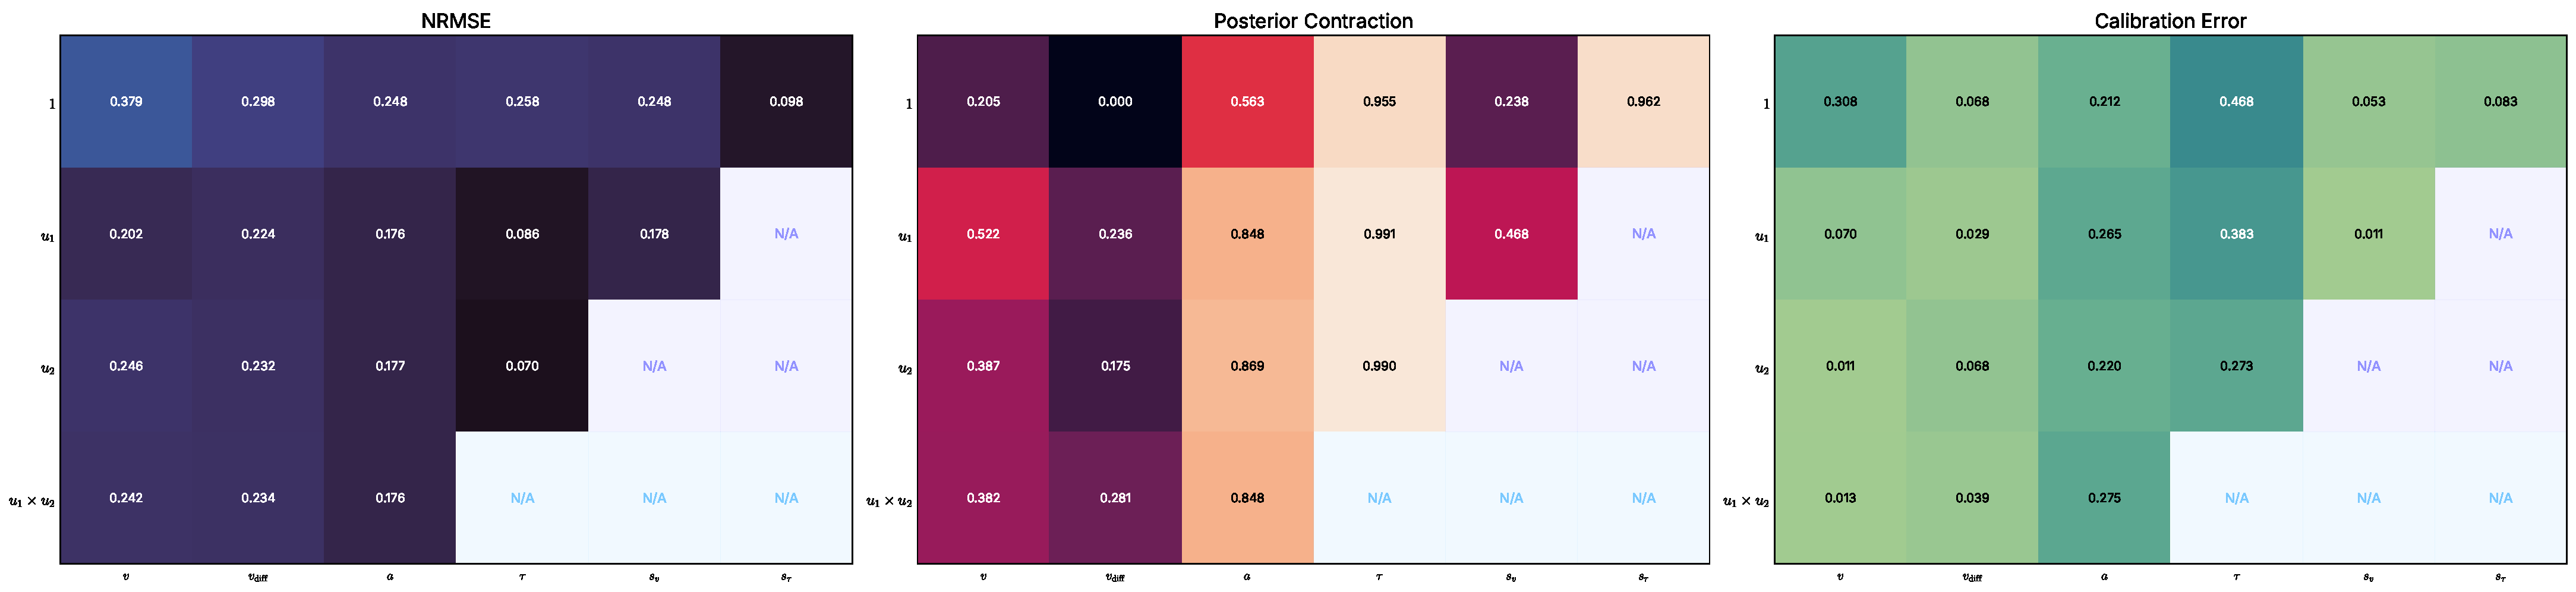
\includegraphics[width=\textwidth]{zeroshot/lba/interaction/metrics.pdf}
    \caption{Metrics}
  \end{subfigure}
  \caption{\textbf{Zero-shot LBA, \emph{interaction} design.} (a) Recovery, (b) calibration, (c) metrics. $v$, $v_{\mathrm{diff}}$, $a$, $\tau$ and $s_v$ carry slopes on $u_1$; $v$, $v_{\mathrm{diff}}$, $a$ and $\tau$ carry slopes on $u_2$; $v$, $v_{\mathrm{diff}}$ and $a$ on the product $u_1 u_2$ (18 coefficients shown). As in Figure~\ref{fig:app3-zeroshot-lba-intercept-only}.}
  \label{fig:app3-zeroshot-lba-interaction}
\end{figure}

\begin{figure}[p]
  \centering
  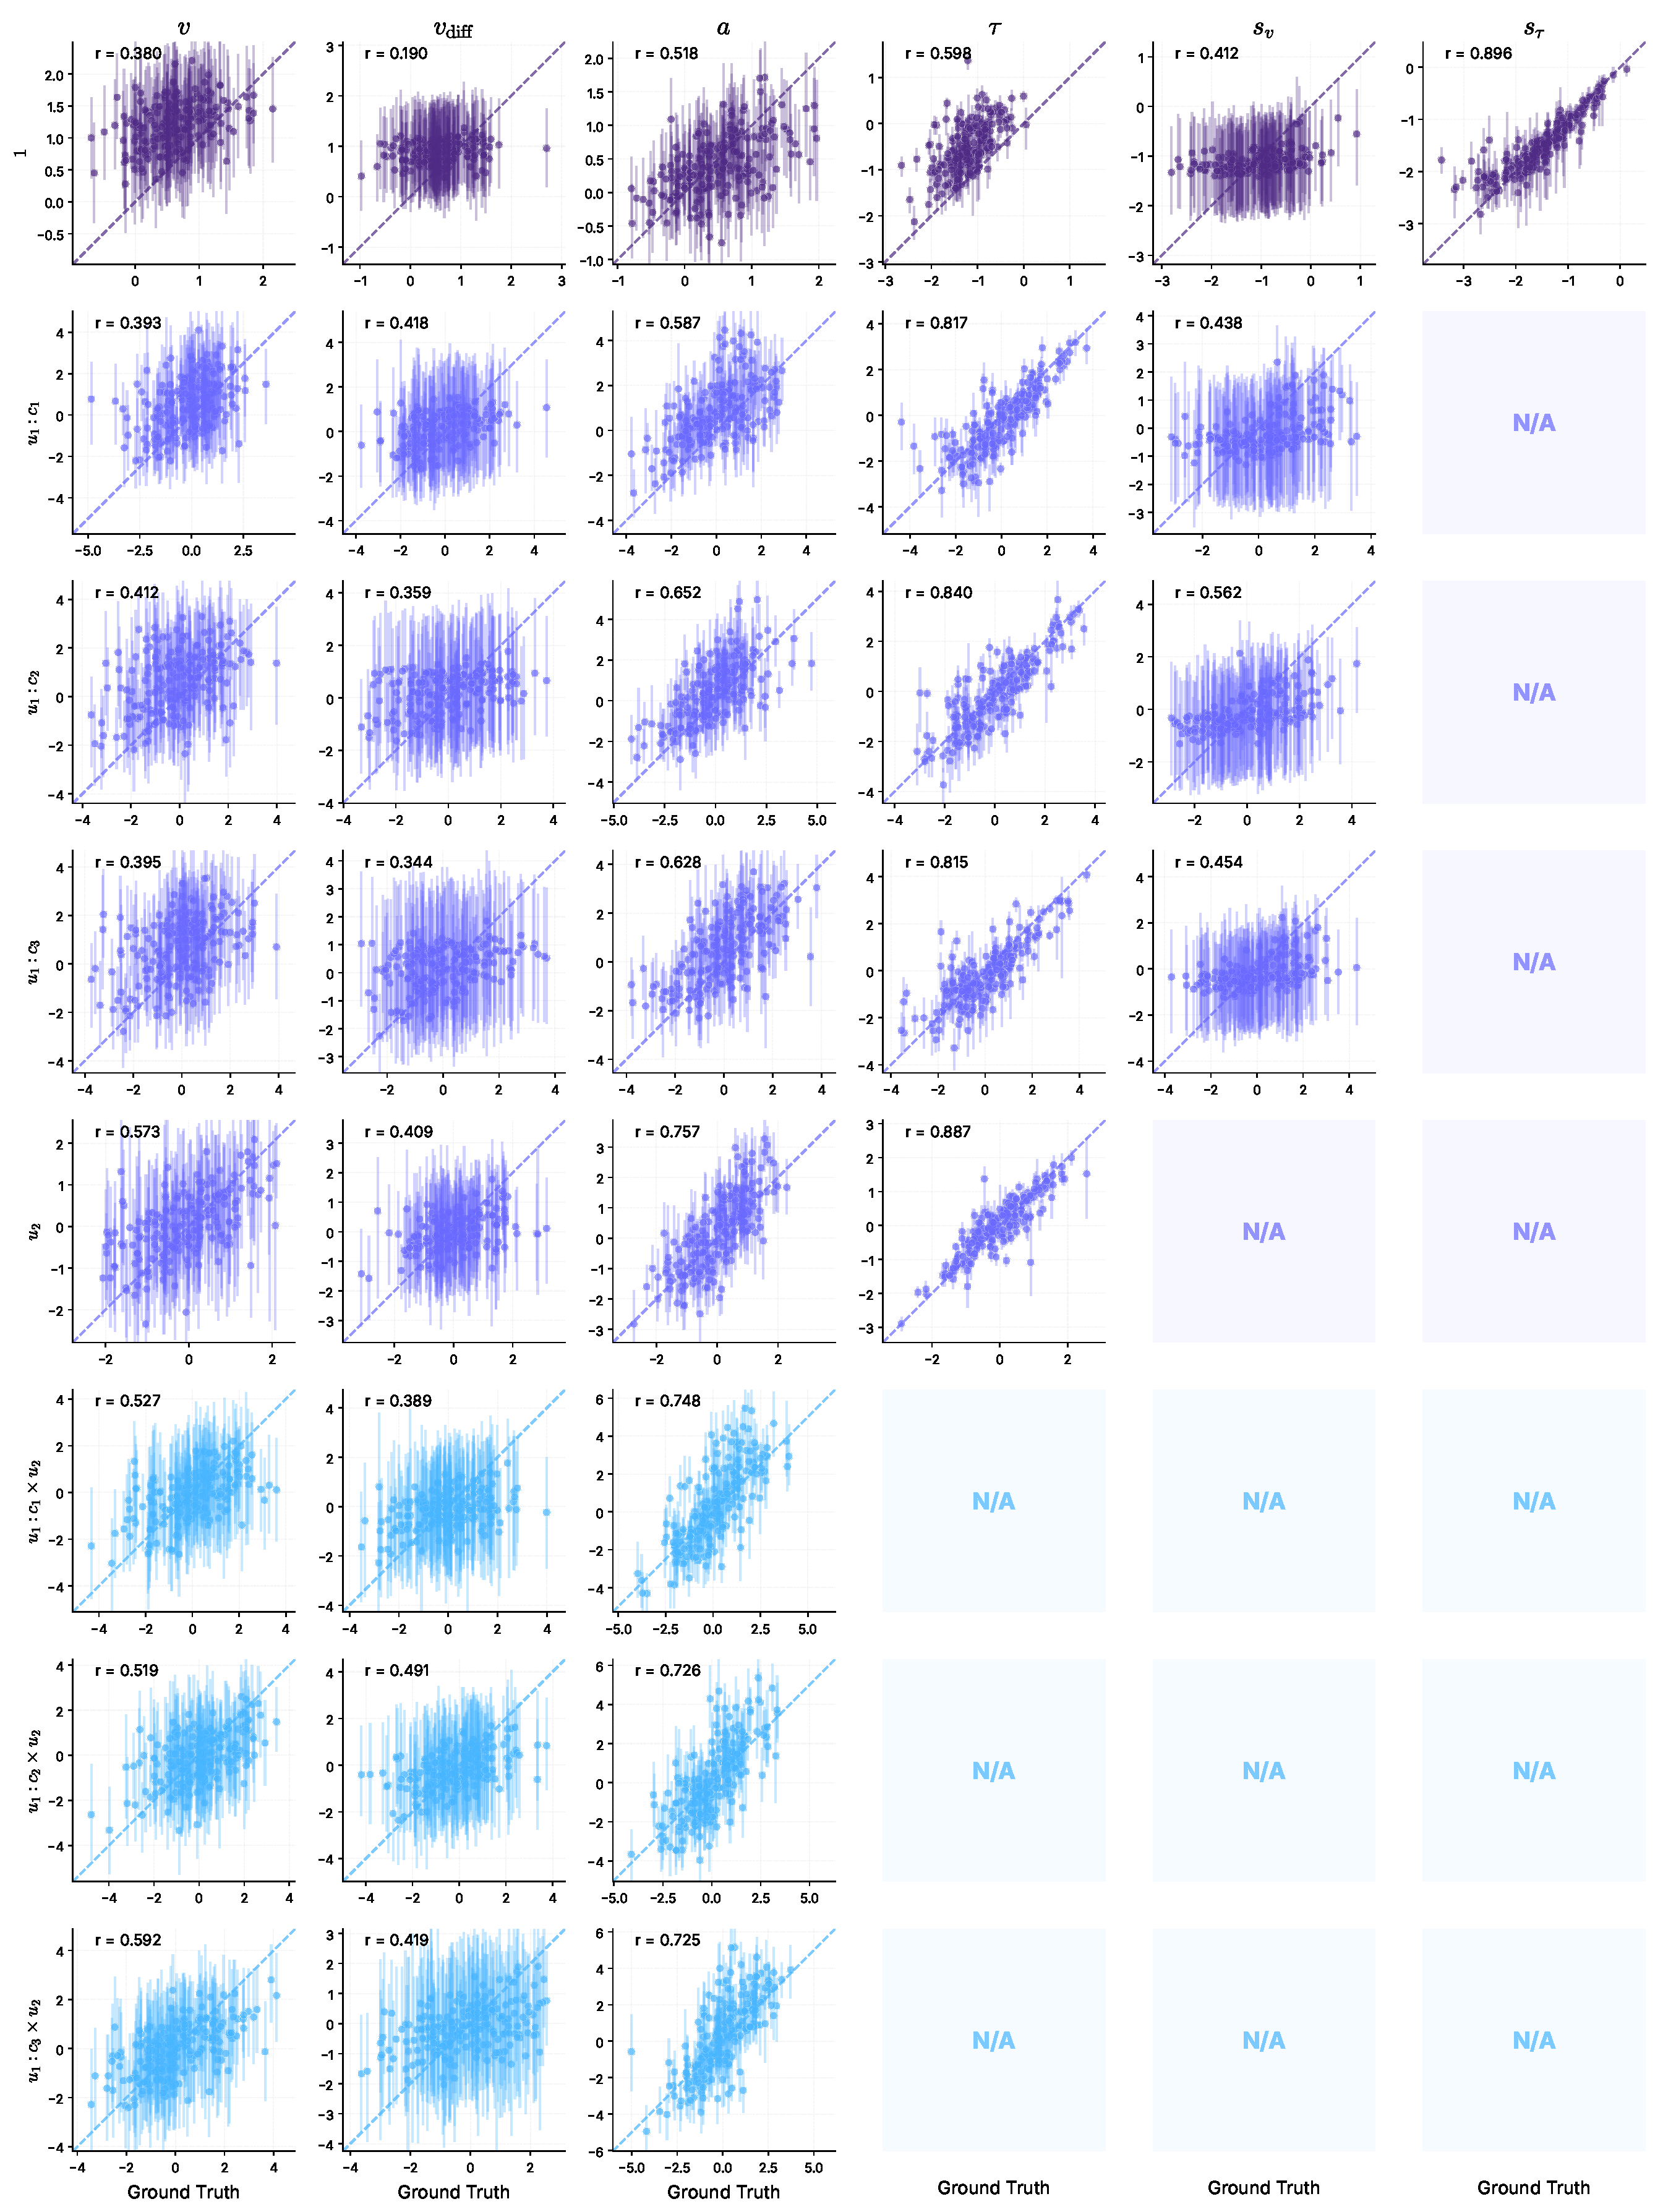
\includegraphics[width=\textwidth,height=0.82\textheight,keepaspectratio]{zeroshot/lba/mixed_predictor/recovery.pdf}
  \caption{\textbf{Parameter recovery, zero-shot LBA, mixed-predictor design.} $v$, $v_{\mathrm{diff}}$, $a$, $\tau$ and $s_v$ carry effects of the four-level $u_1$; $v$, $v_{\mathrm{diff}}$, $a$ and $\tau$ slopes on $u_2$; $v$, $v_{\mathrm{diff}}$ and $a$ the interaction (34 coefficients shown). Datasets simulated for this design (no shared benchmark file exists); design as in Figure~\ref{fig:app1-ddm-mixed-predictor-recovery}, encoding as in the top panel of Figure~\ref{fig:app1-ddm-intercept-only-cf}.}
  \label{fig:app3-zeroshot-lba-mixed-predictor-recovery}
\end{figure}

\begin{figure}[p]
  \centering
  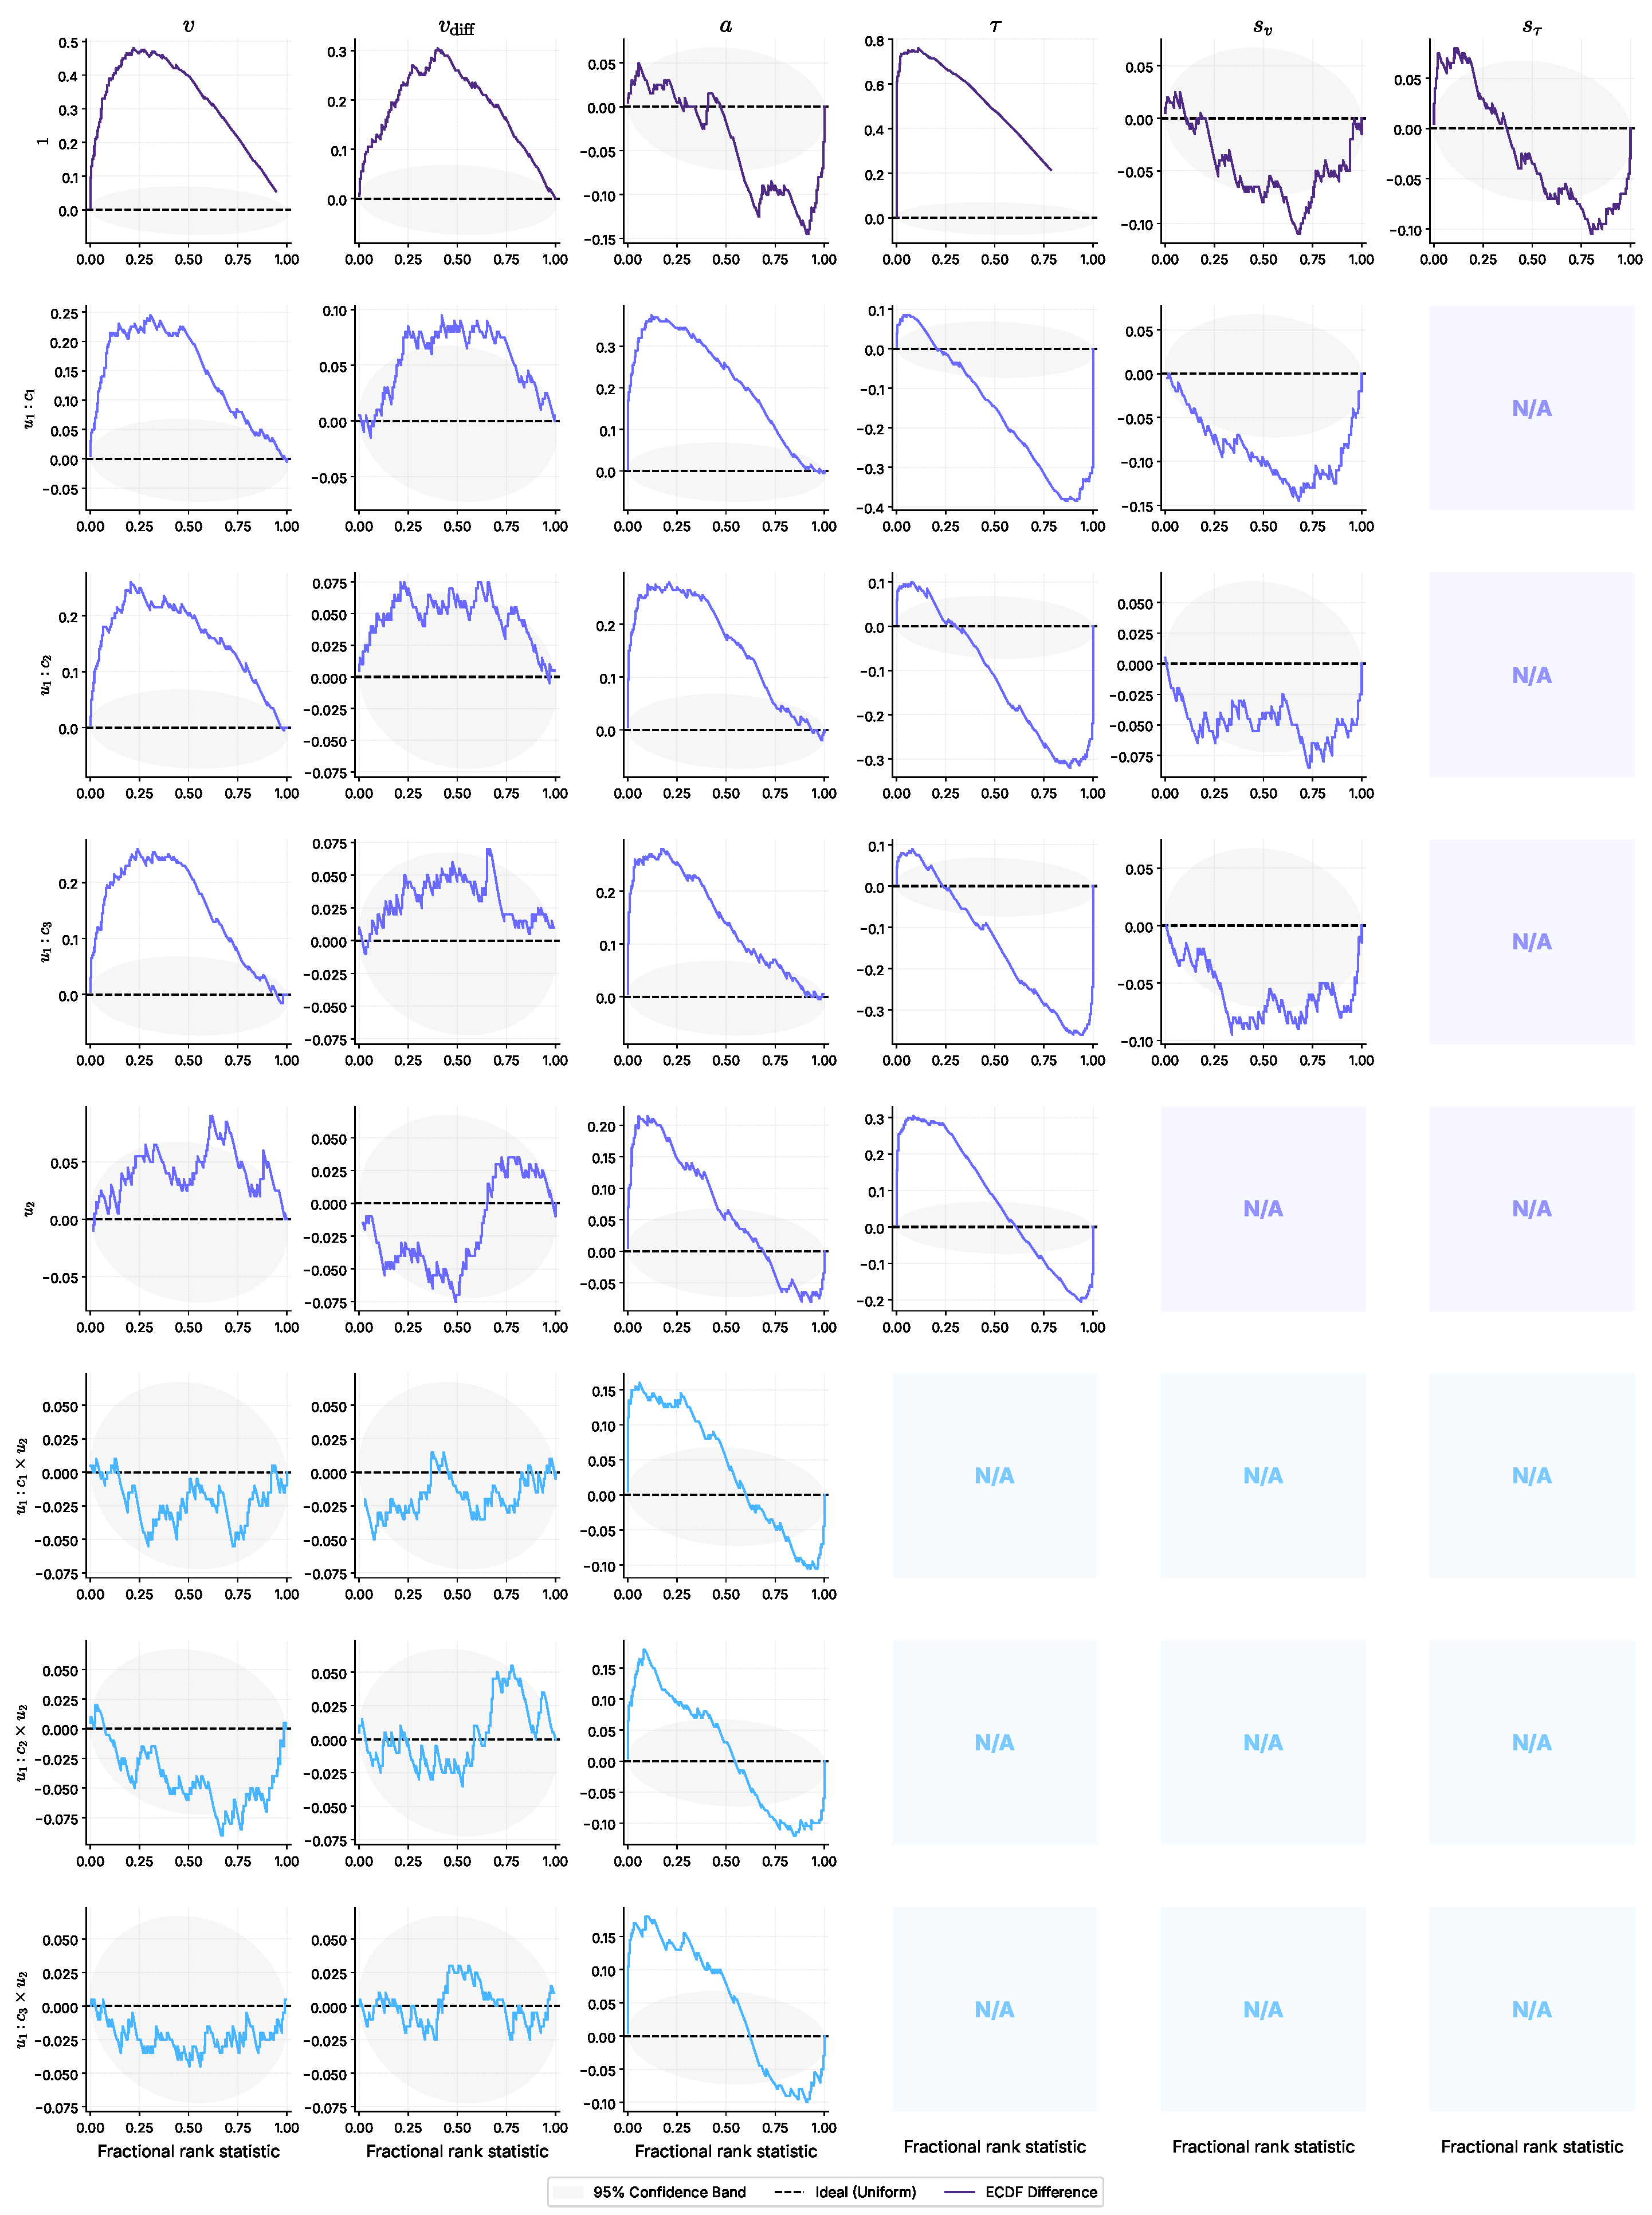
\includegraphics[width=\textwidth,height=0.82\textheight,keepaspectratio]{zeroshot/lba/mixed_predictor/ecdf.pdf}
  \caption{\textbf{Simulation-based calibration, zero-shot LBA, mixed-predictor design.} $v$, $v_{\mathrm{diff}}$, $a$, $\tau$ and $s_v$ carry effects of the four-level $u_1$; $v$, $v_{\mathrm{diff}}$, $a$ and $\tau$ slopes on $u_2$; $v$, $v_{\mathrm{diff}}$ and $a$ the interaction (34 coefficients shown). Datasets simulated for this design (no shared benchmark file exists); design as in Figure~\ref{fig:app1-ddm-mixed-predictor-recovery}, encoding as in the middle panel of Figure~\ref{fig:app1-ddm-intercept-only-cf}.}
  \label{fig:app3-zeroshot-lba-mixed-predictor-ecdf}
\end{figure}

\begin{figure}[p]
  \centering
  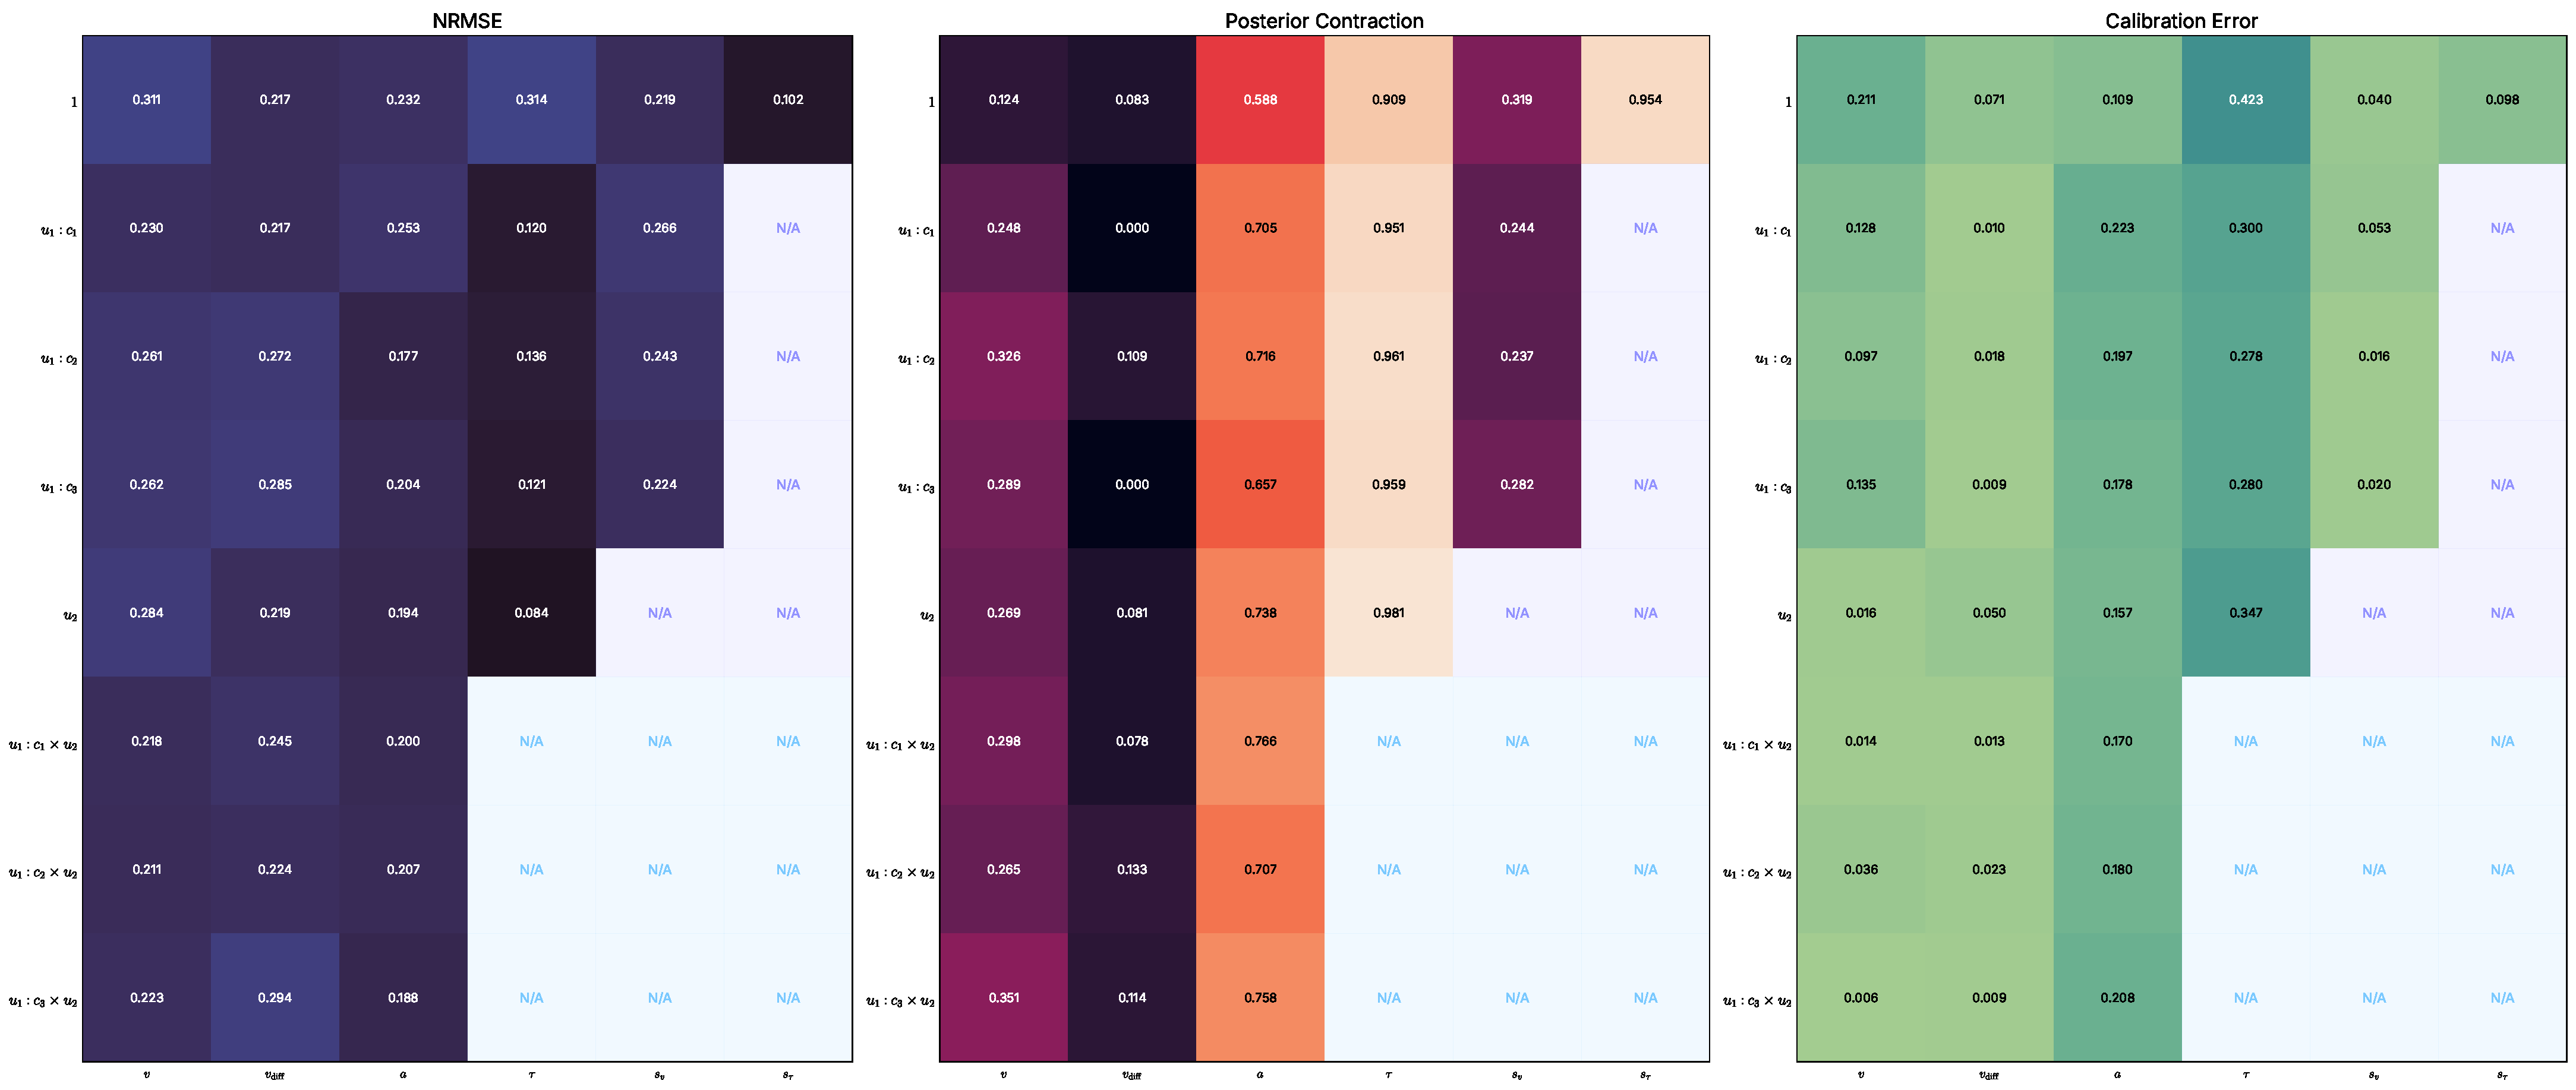
\includegraphics[width=\textwidth,height=0.82\textheight,keepaspectratio]{zeroshot/lba/mixed_predictor/metrics.pdf}
  \caption{\textbf{Summary metrics, zero-shot LBA, mixed-predictor design.} $v$, $v_{\mathrm{diff}}$, $a$, $\tau$ and $s_v$ carry effects of the four-level $u_1$; $v$, $v_{\mathrm{diff}}$, $a$ and $\tau$ slopes on $u_2$; $v$, $v_{\mathrm{diff}}$ and $a$ the interaction (34 coefficients shown). Datasets simulated for this design (no shared benchmark file exists); design as in Figure~\ref{fig:app1-ddm-mixed-predictor-recovery}, encoding as in the bottom panel of Figure~\ref{fig:app1-ddm-intercept-only-cf}.}
  \label{fig:app3-zeroshot-lba-mixed-predictor-metrics}
\end{figure}

% ── 2. after fine-tuning ──

\begin{figure}[p]
  \centering
  \begin{subfigure}{\textwidth}\centering
    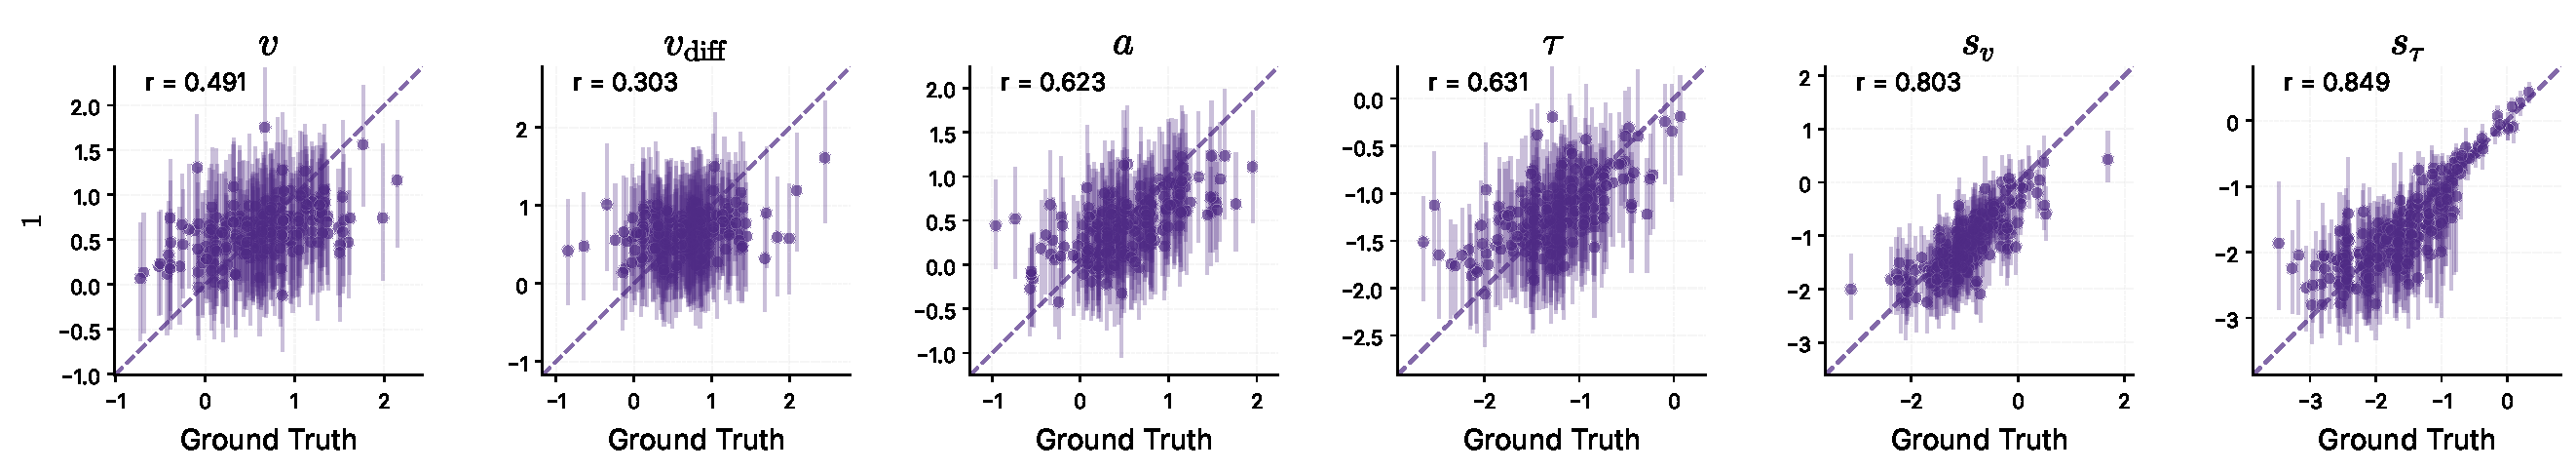
\includegraphics[width=\textwidth,height=0.3\textheight,keepaspectratio]{finetuned/lba/intercept_only/recovery.pdf}
    \caption{Recovery}
  \end{subfigure}\\[1ex]
  \begin{subfigure}{\textwidth}\centering
    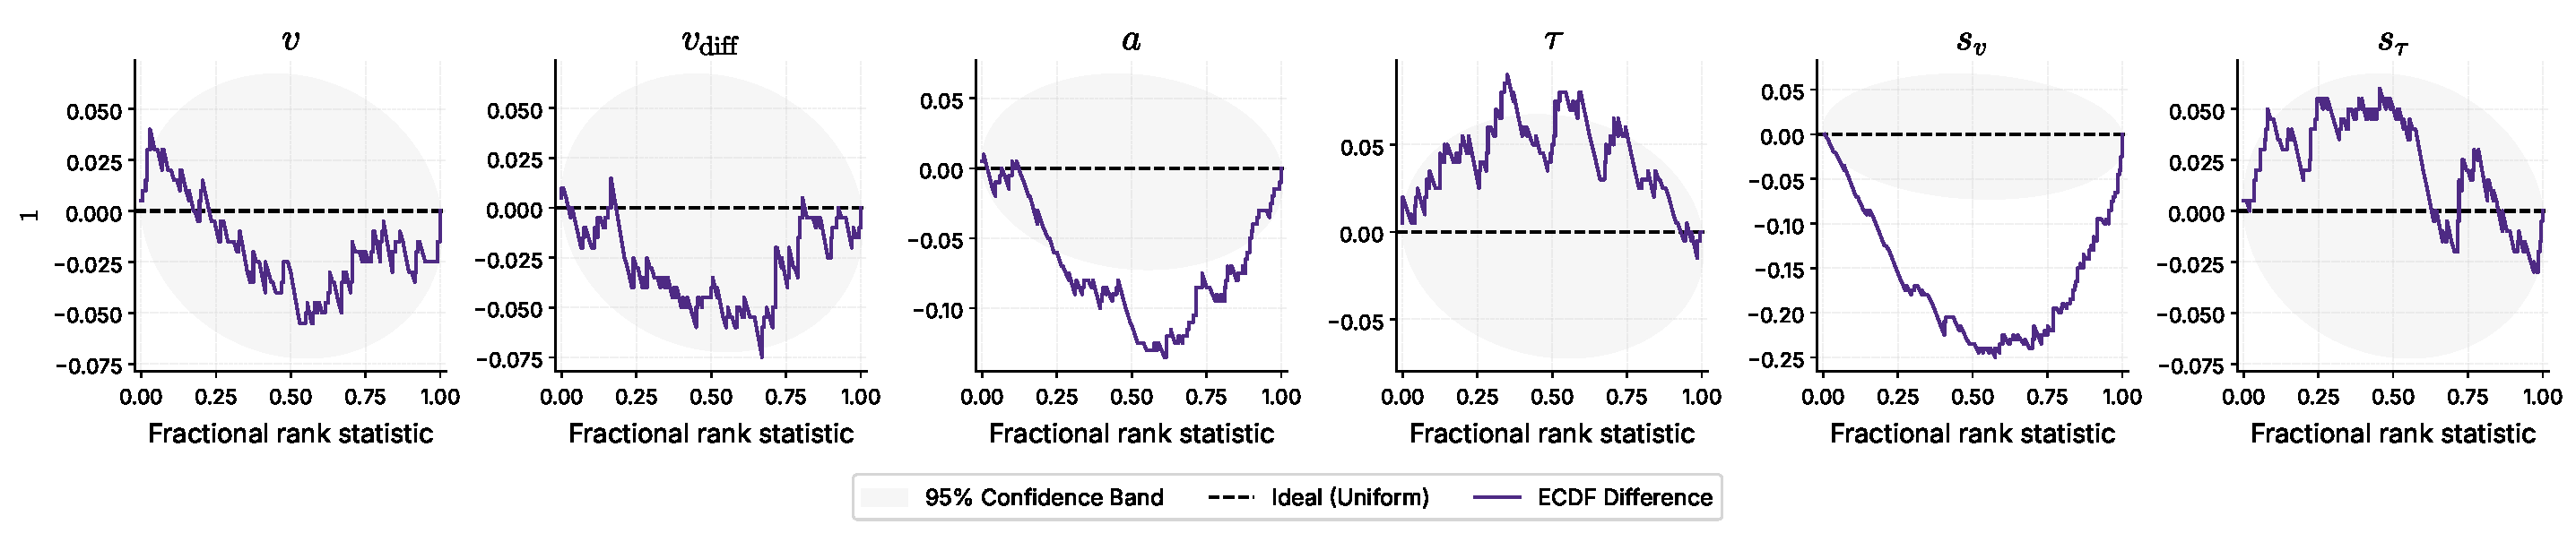
\includegraphics[width=\textwidth,height=0.3\textheight,keepaspectratio]{finetuned/lba/intercept_only/ecdf.pdf}
    \caption{Calibration (ECDF)}
  \end{subfigure}\\[1ex]
  \begin{subfigure}{\textwidth}\centering
    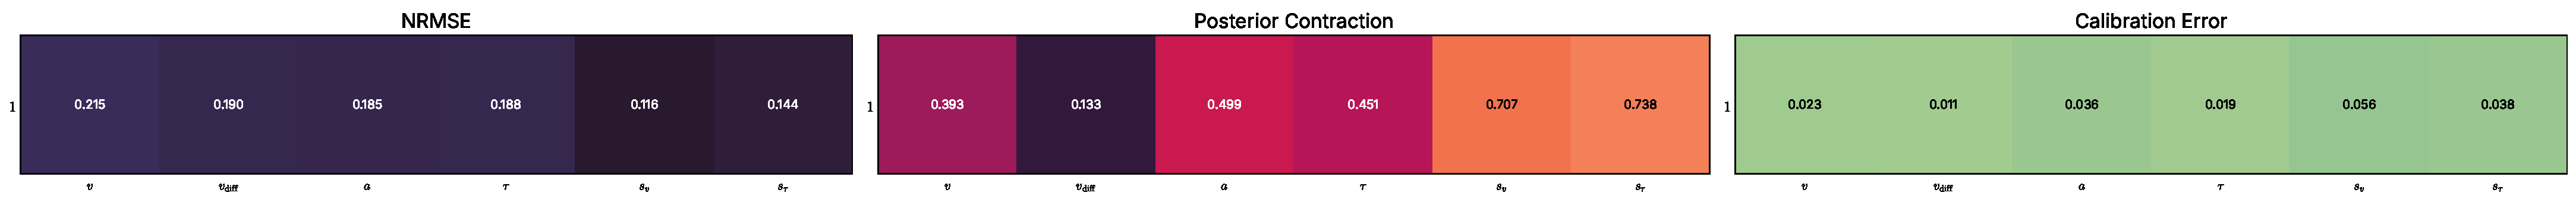
\includegraphics[width=\textwidth]{finetuned/lba/intercept_only/metrics.pdf}
    \caption{Metrics}
  \end{subfigure}
  \caption{\textbf{After fine-tuning: LBA, \emph{intercept-only} design.} (a) Recovery, (b) calibration and (c) summary metrics of the network after 1000 epochs of fine-tuning on all four families jointly (DDM, RDM, CDM and LBA, drawn with equal probability), the LBA now under its own model embedding, initialised from the RDM's. Same test datasets, draws and encoding as Figure~\ref{fig:app3-zeroshot-lba-intercept-only}, so each figure compares directly with its zero-shot counterpart. Every estimated parameter enters as an intercept only (6 coefficients shown). The same diagnostics for DDM, RDM and CDM after fine-tuning (Figures~\ref{fig:app3-finetuned-ddm-intercept-only}--\ref{fig:app3-finetuned-cdm-mixed-predictor-metrics}) quantify forgetting: compare them with the original network on the identical bench5 datasets (Figure~\ref{fig:app1-ddm-intercept-only-cf} and the following CogFormer figures).}
  \label{fig:app3-finetuned-lba-intercept-only}
\end{figure}

\begin{figure}[p]
  \centering
  \begin{subfigure}{\textwidth}\centering
    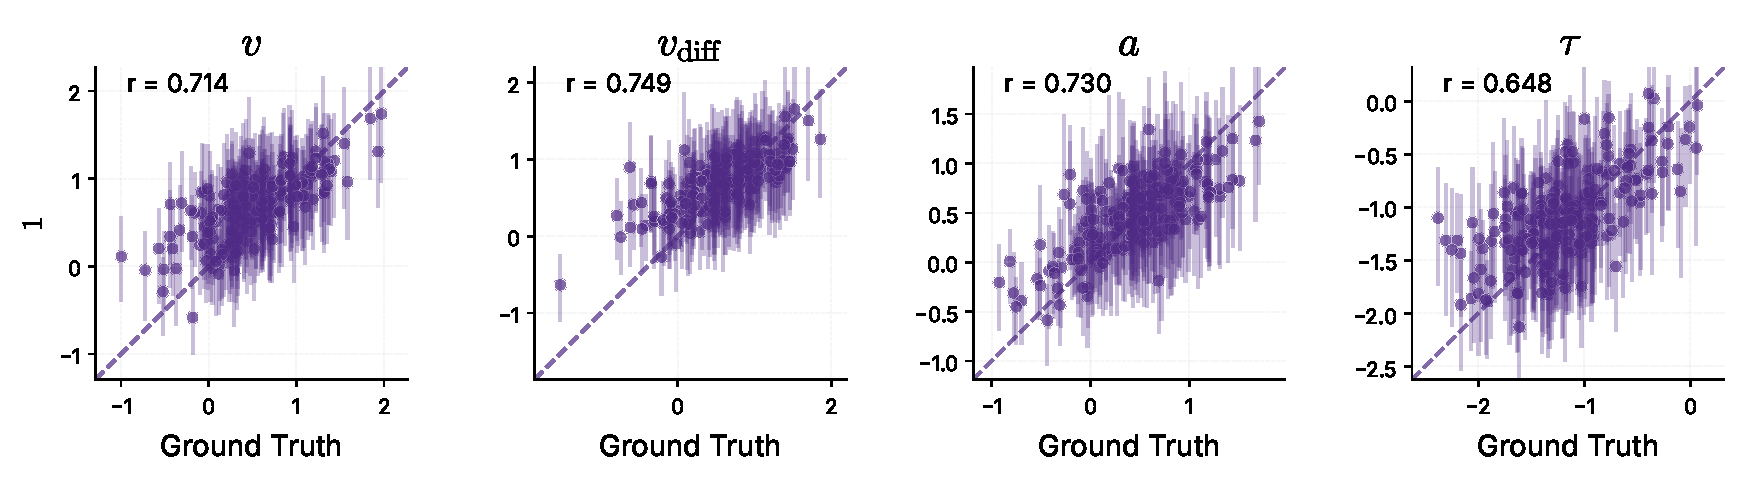
\includegraphics[width=\textwidth,height=0.3\textheight,keepaspectratio]{finetuned/lba/fixed/recovery.pdf}
    \caption{Recovery}
  \end{subfigure}\\[1ex]
  \begin{subfigure}{\textwidth}\centering
    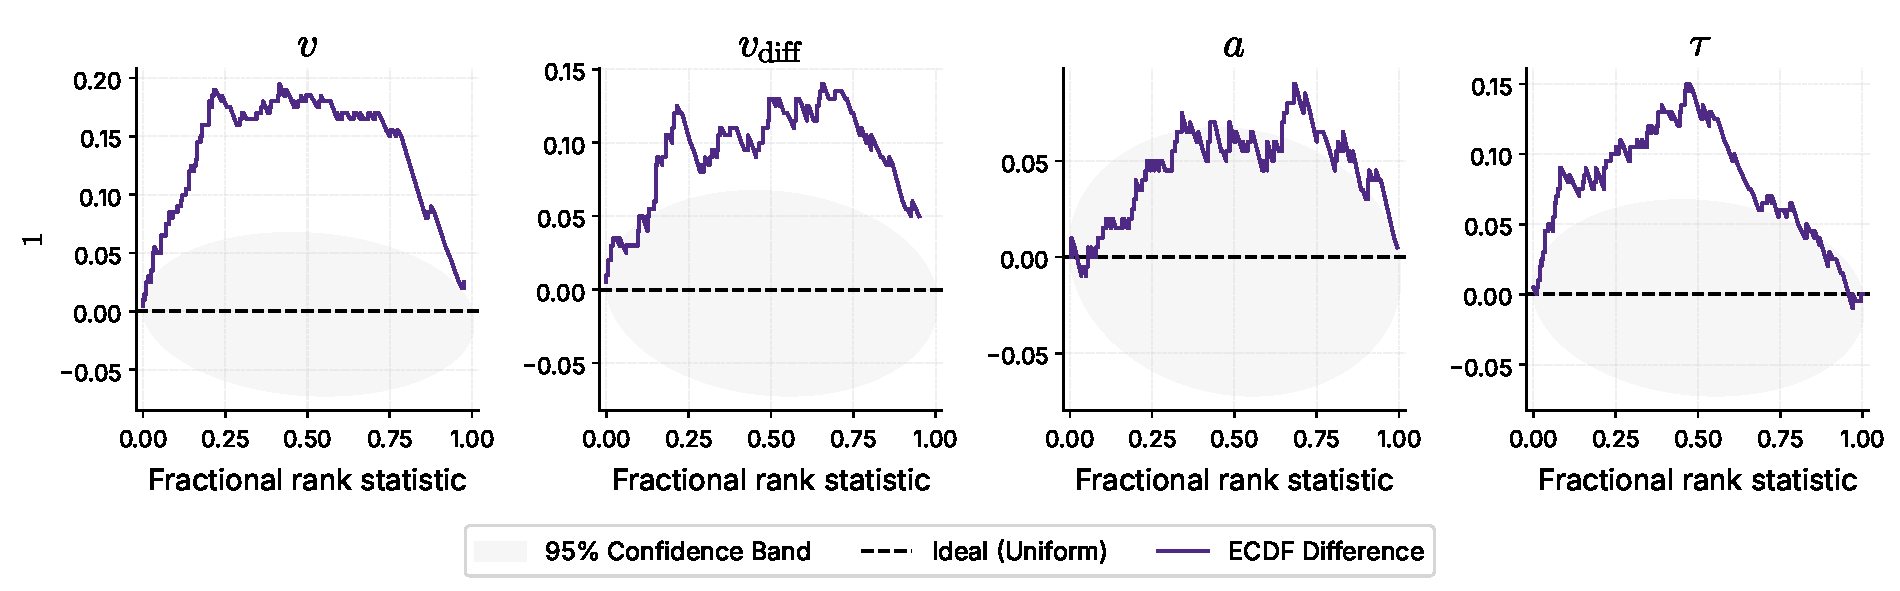
\includegraphics[width=\textwidth,height=0.3\textheight,keepaspectratio]{finetuned/lba/fixed/ecdf.pdf}
    \caption{Calibration (ECDF)}
  \end{subfigure}\\[1ex]
  \begin{subfigure}{\textwidth}\centering
    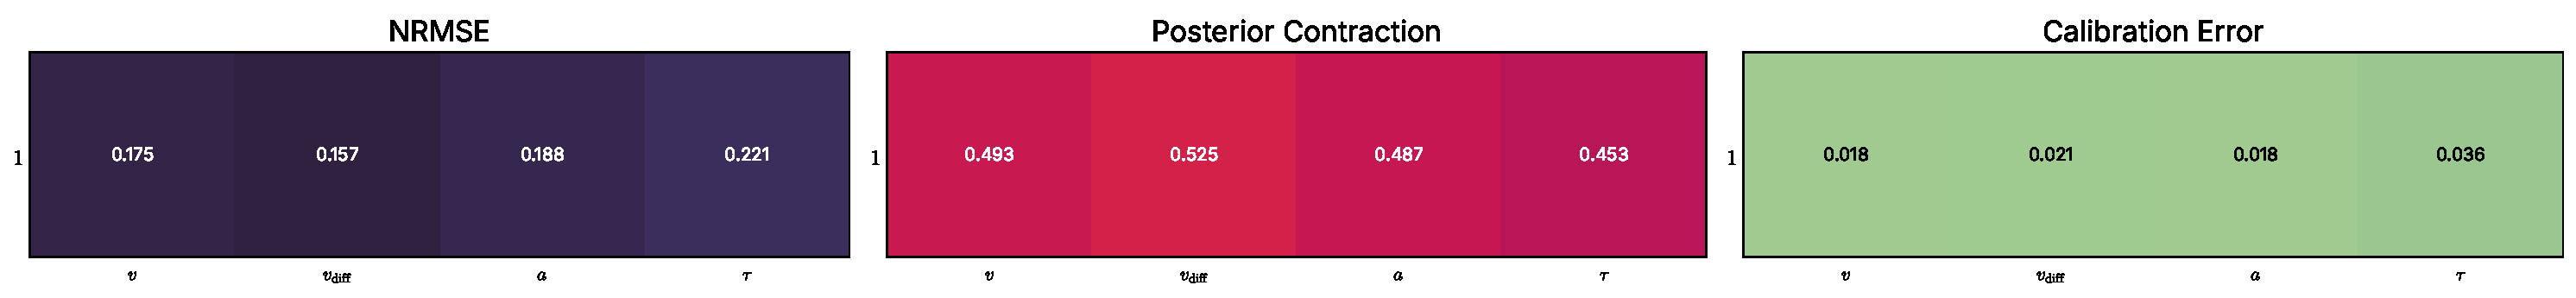
\includegraphics[width=\textwidth]{finetuned/lba/fixed/metrics.pdf}
    \caption{Metrics}
  \end{subfigure}
  \caption{\textbf{After fine-tuning: LBA, \emph{fixed} design.} (a) Recovery, (b) calibration, (c) metrics. $s_v$ and $s_\tau$ are fixed at 0 and not estimated; every estimated parameter enters as an intercept only (4 coefficients shown). As in Figure~\ref{fig:app3-finetuned-lba-intercept-only}; zero-shot counterpart: Figure~\ref{fig:app3-zeroshot-lba-fixed}.}
  \label{fig:app3-finetuned-lba-fixed}
\end{figure}

\begin{figure}[p]
  \centering
  \begin{subfigure}{\textwidth}\centering
    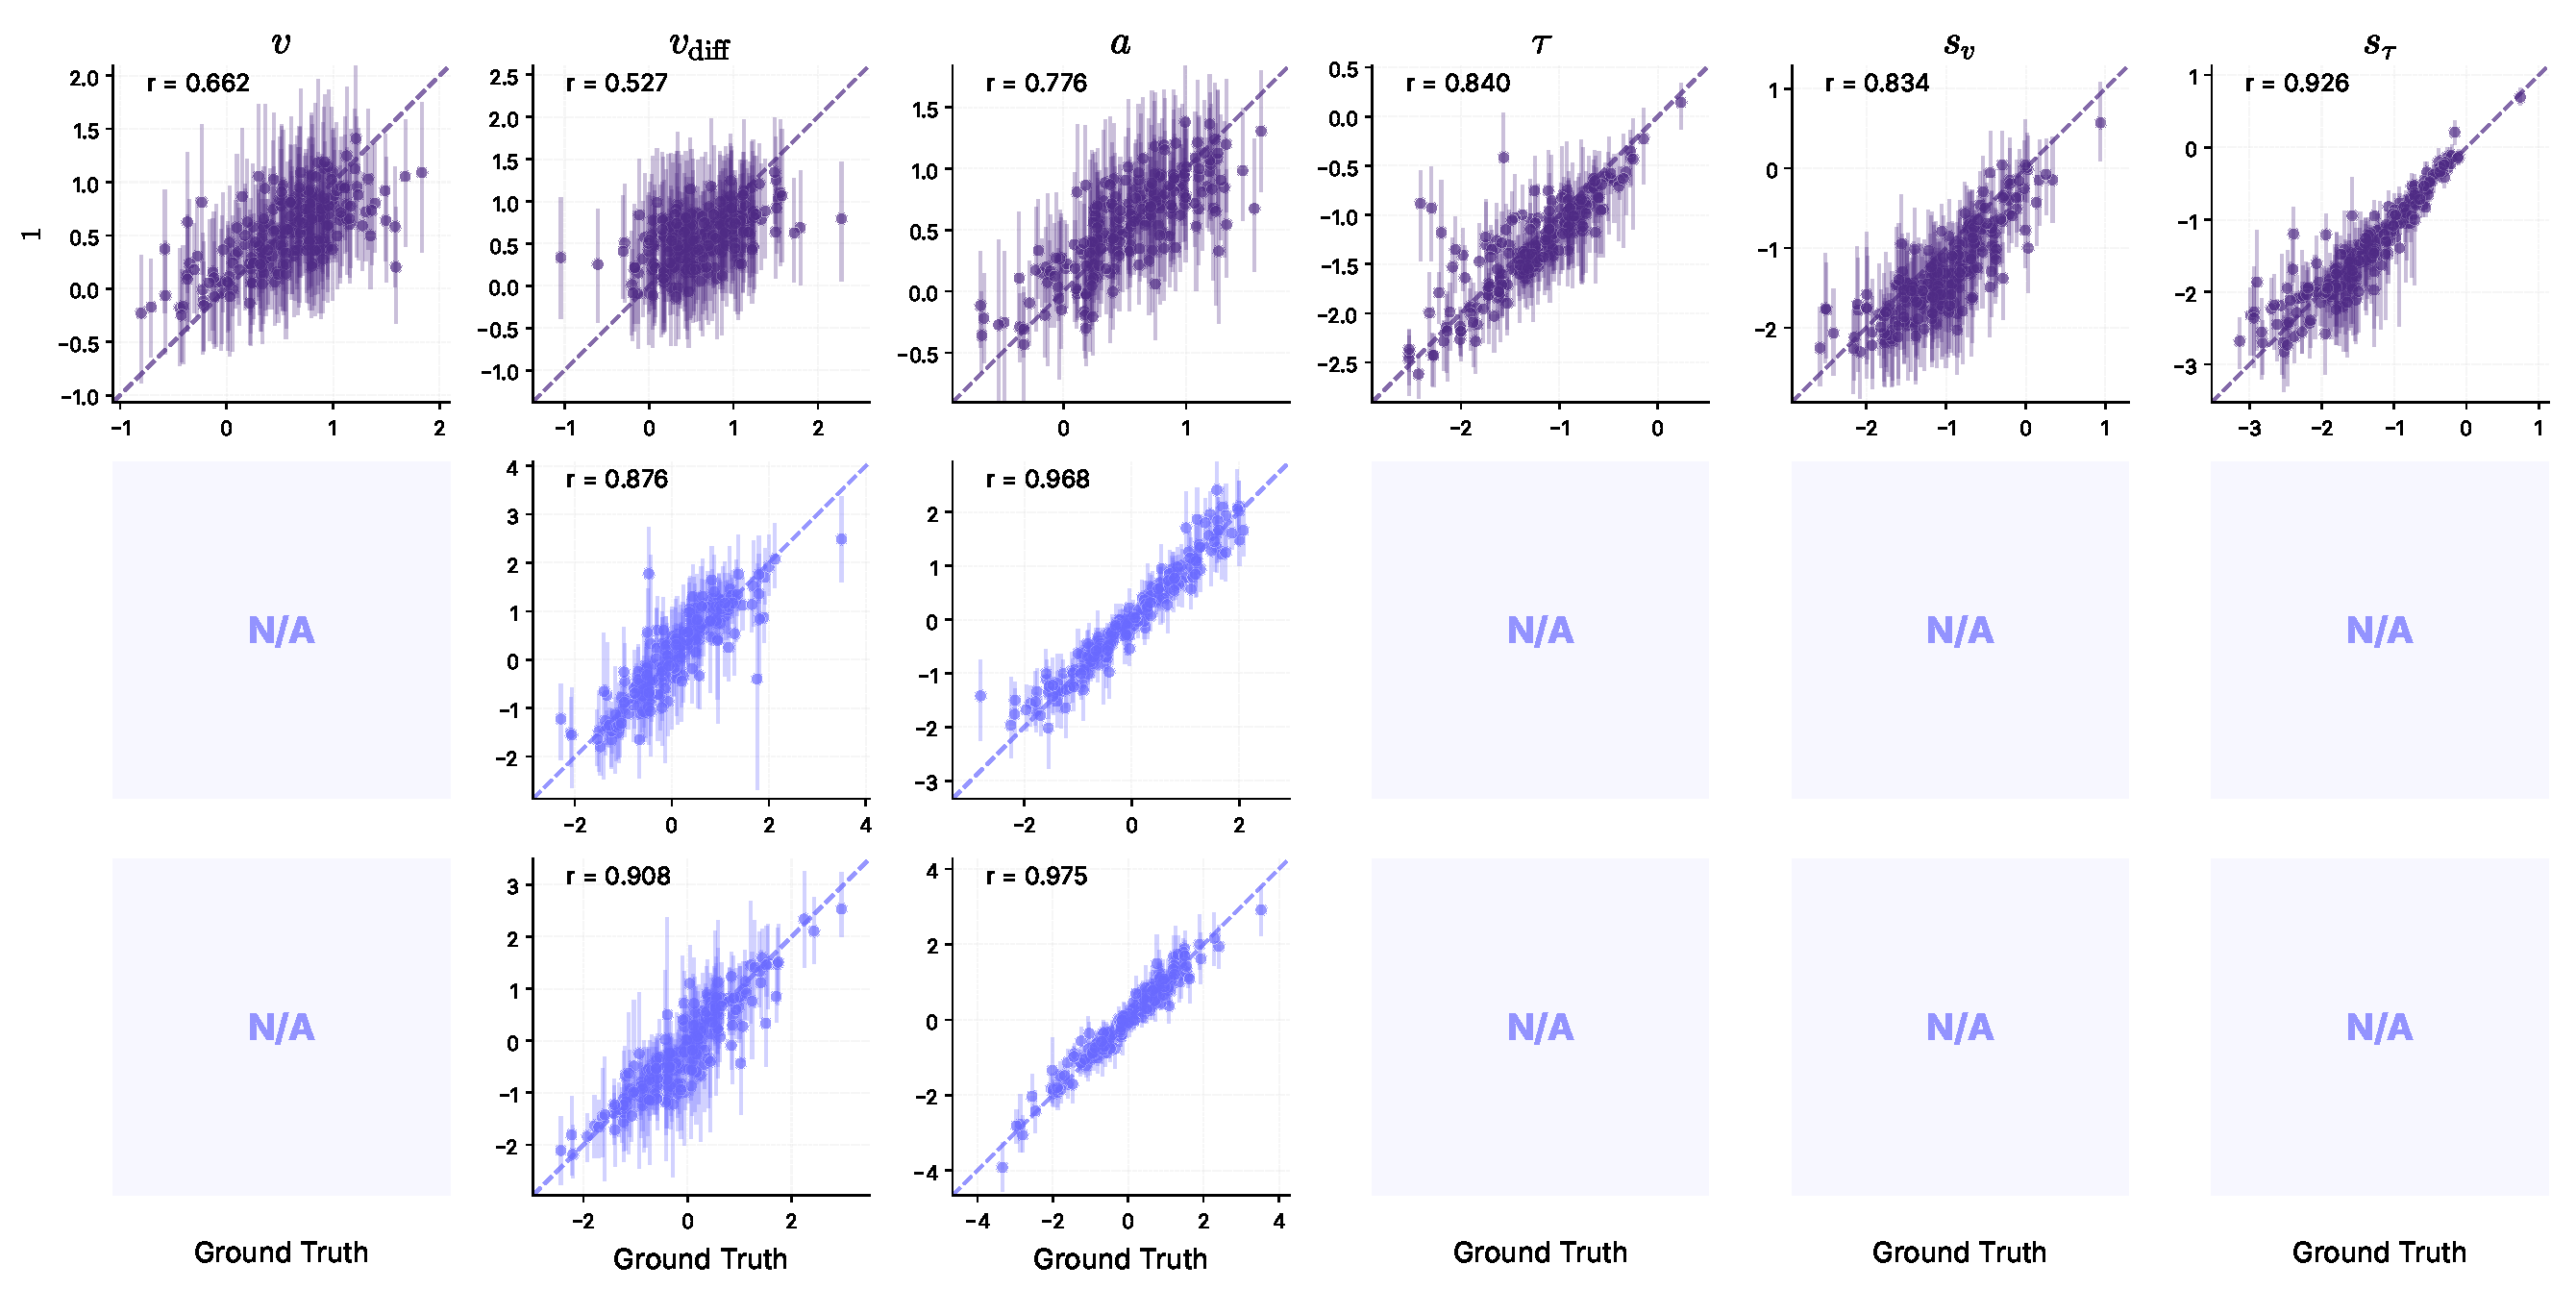
\includegraphics[width=\textwidth,height=0.3\textheight,keepaspectratio]{finetuned/lba/regressed/recovery.pdf}
    \caption{Recovery}
  \end{subfigure}\\[1ex]
  \begin{subfigure}{\textwidth}\centering
    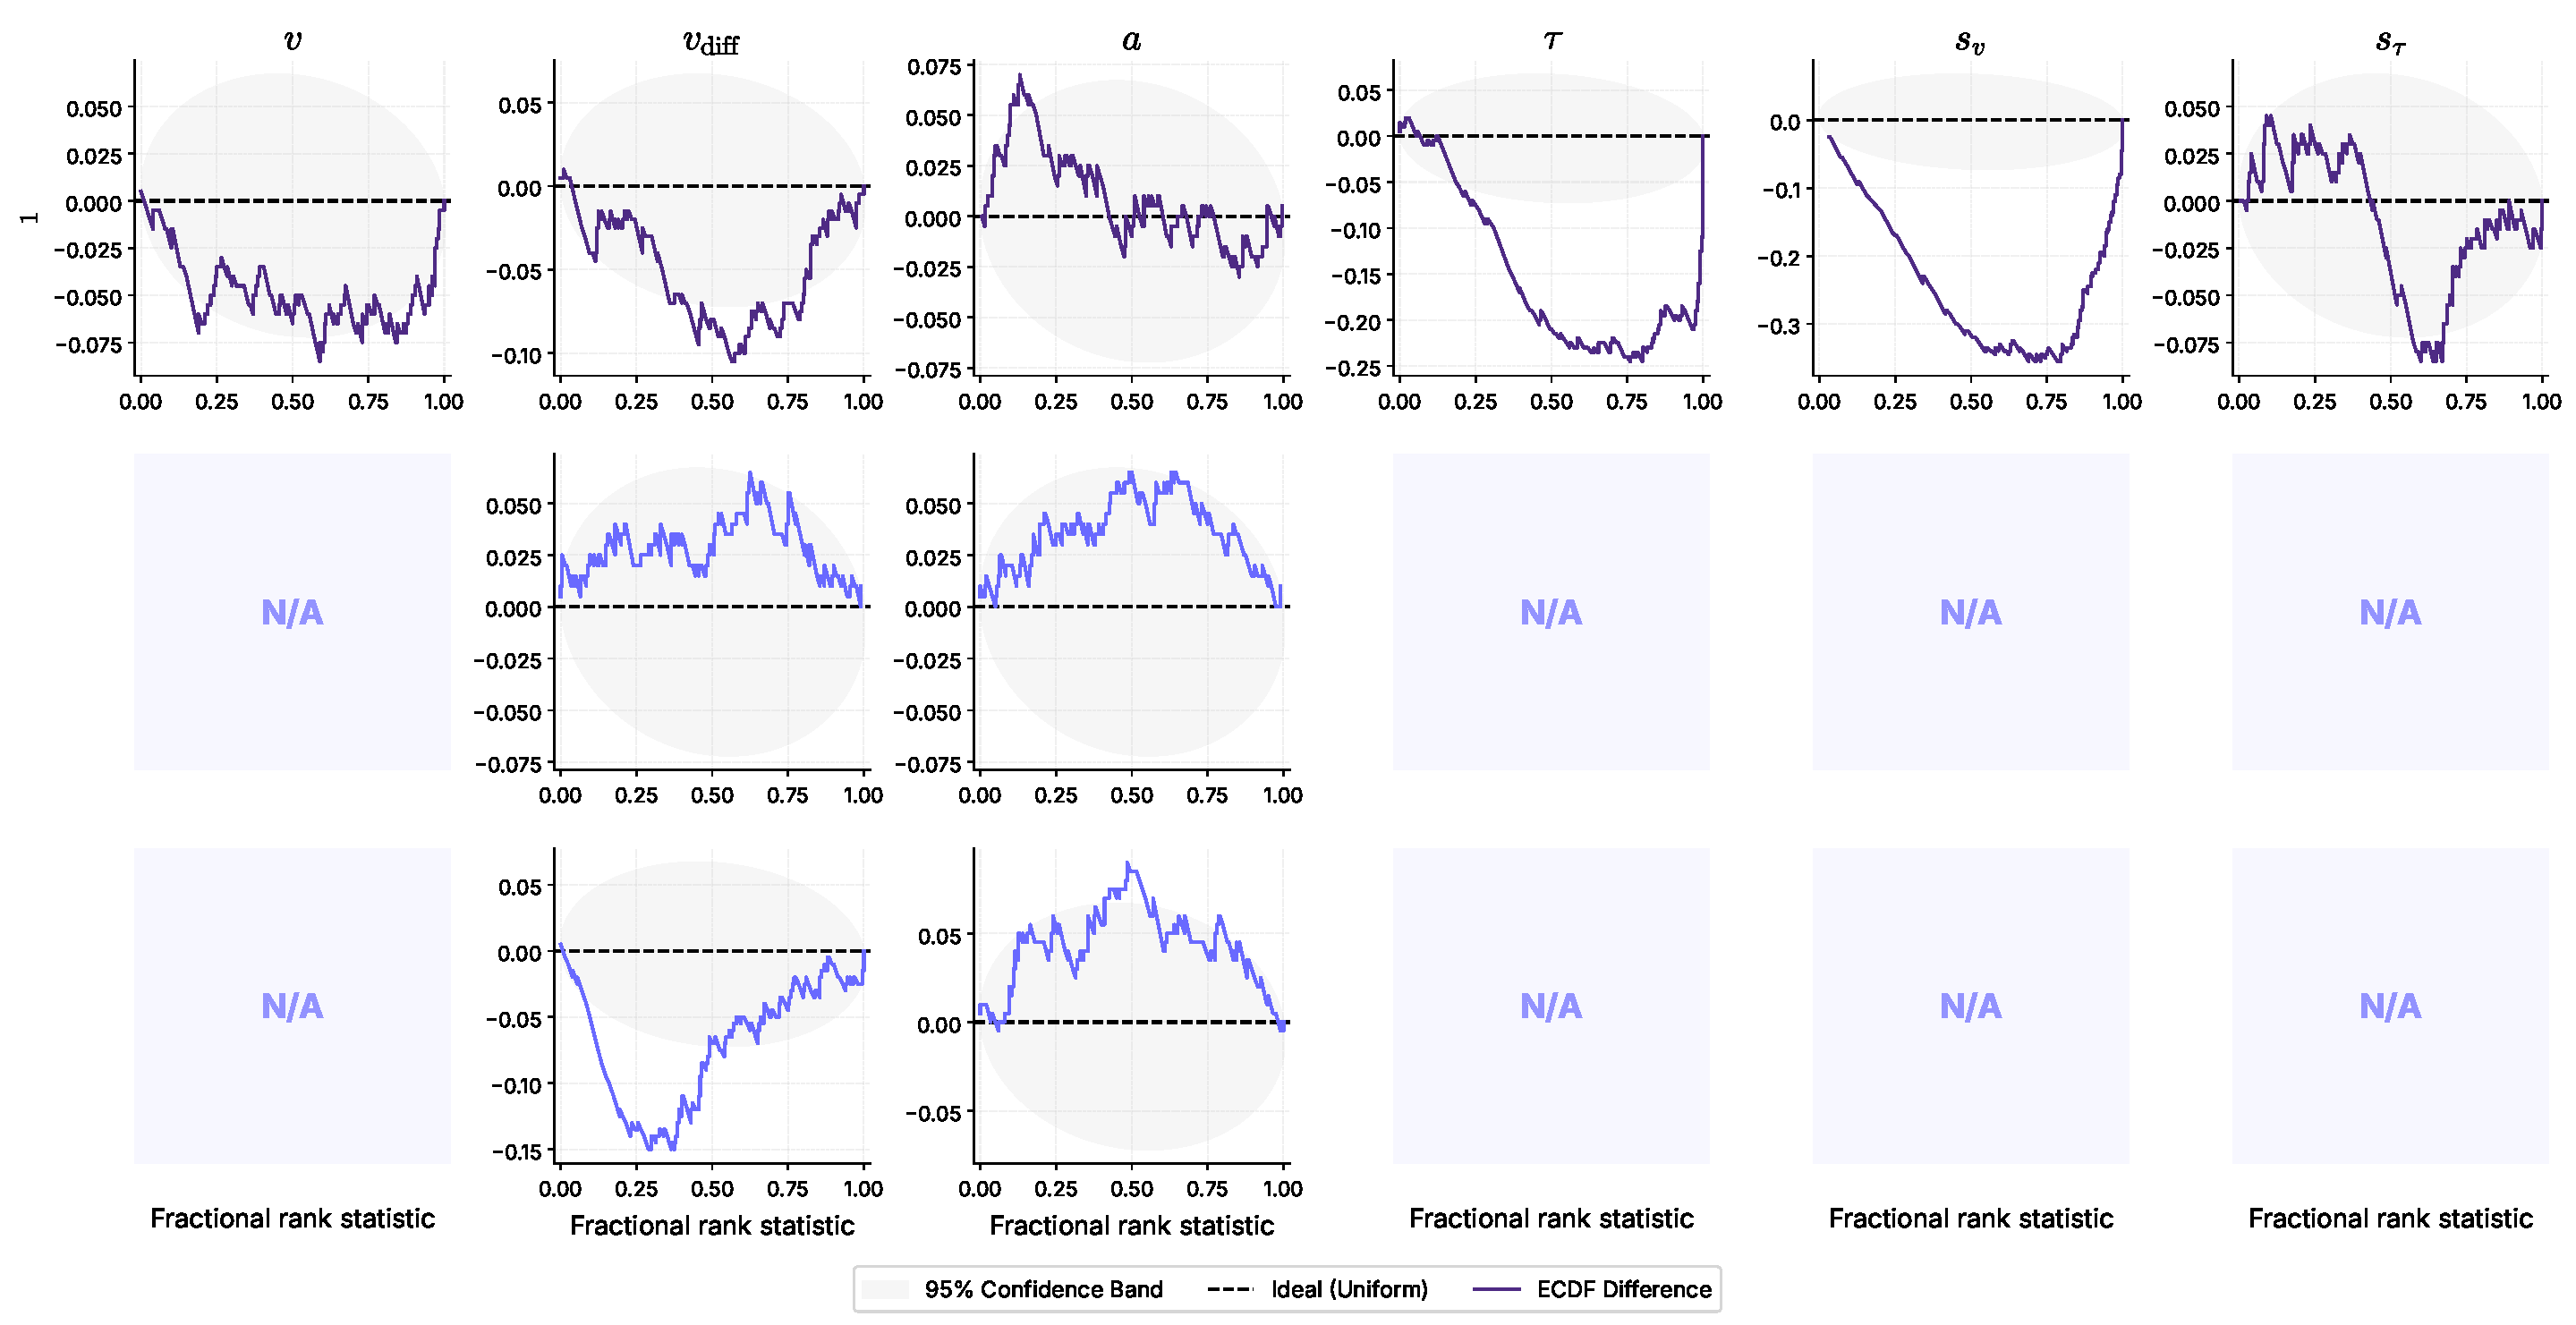
\includegraphics[width=\textwidth,height=0.3\textheight,keepaspectratio]{finetuned/lba/regressed/ecdf.pdf}
    \caption{Calibration (ECDF)}
  \end{subfigure}\\[1ex]
  \begin{subfigure}{\textwidth}\centering
    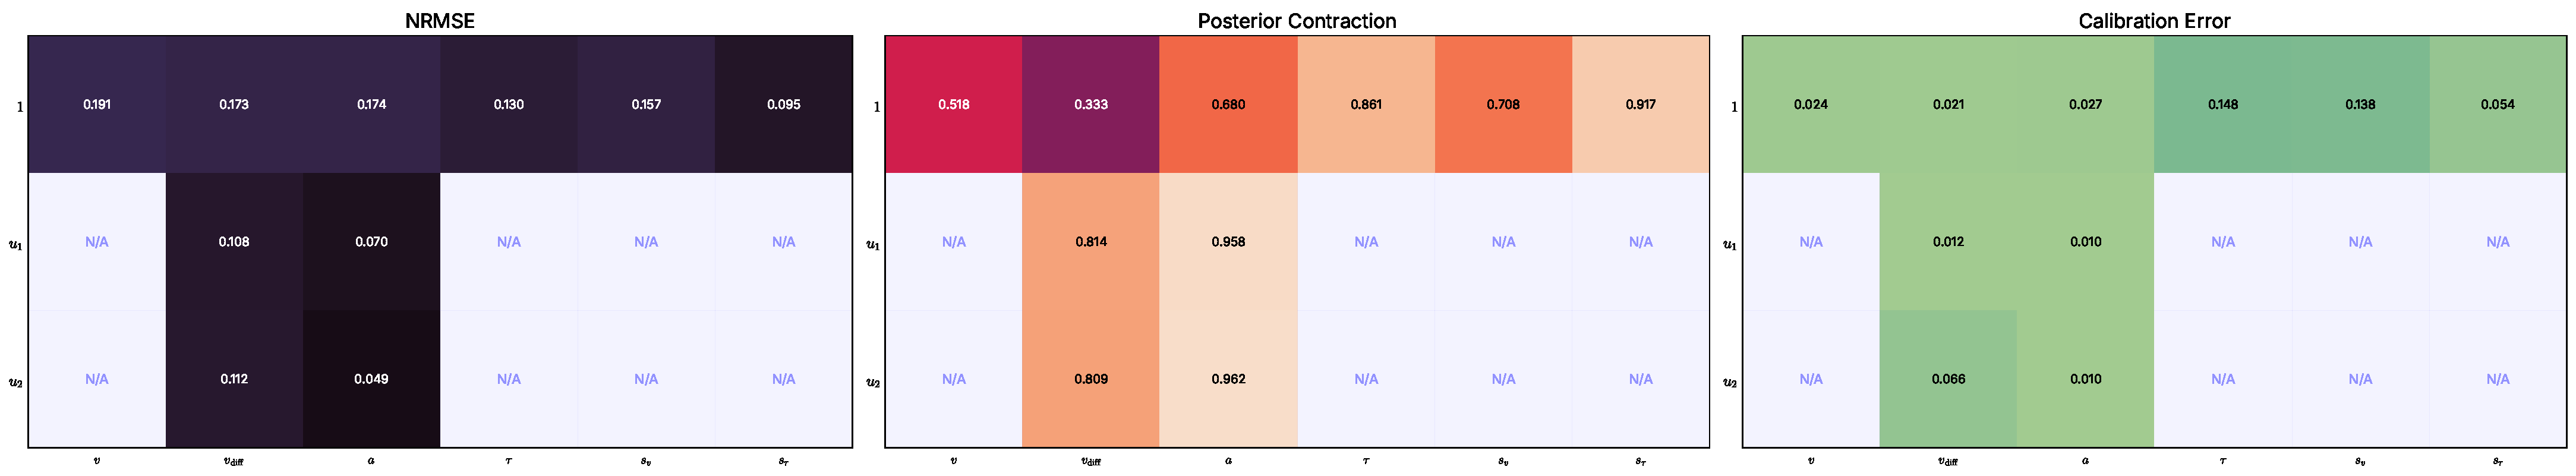
\includegraphics[width=\textwidth]{finetuned/lba/regressed/metrics.pdf}
    \caption{Metrics}
  \end{subfigure}
  \caption{\textbf{After fine-tuning: LBA, \emph{regressed} design.} (a) Recovery, (b) calibration, (c) metrics. $v_{\mathrm{diff}}$ and $a$ carry slopes on $u_1$ and $u_2$ (10 coefficients shown). As in Figure~\ref{fig:app3-finetuned-lba-intercept-only}; zero-shot counterpart: Figure~\ref{fig:app3-zeroshot-lba-regressed}.}
  \label{fig:app3-finetuned-lba-regressed}
\end{figure}

\begin{figure}[p]
  \centering
  \begin{subfigure}{\textwidth}\centering
    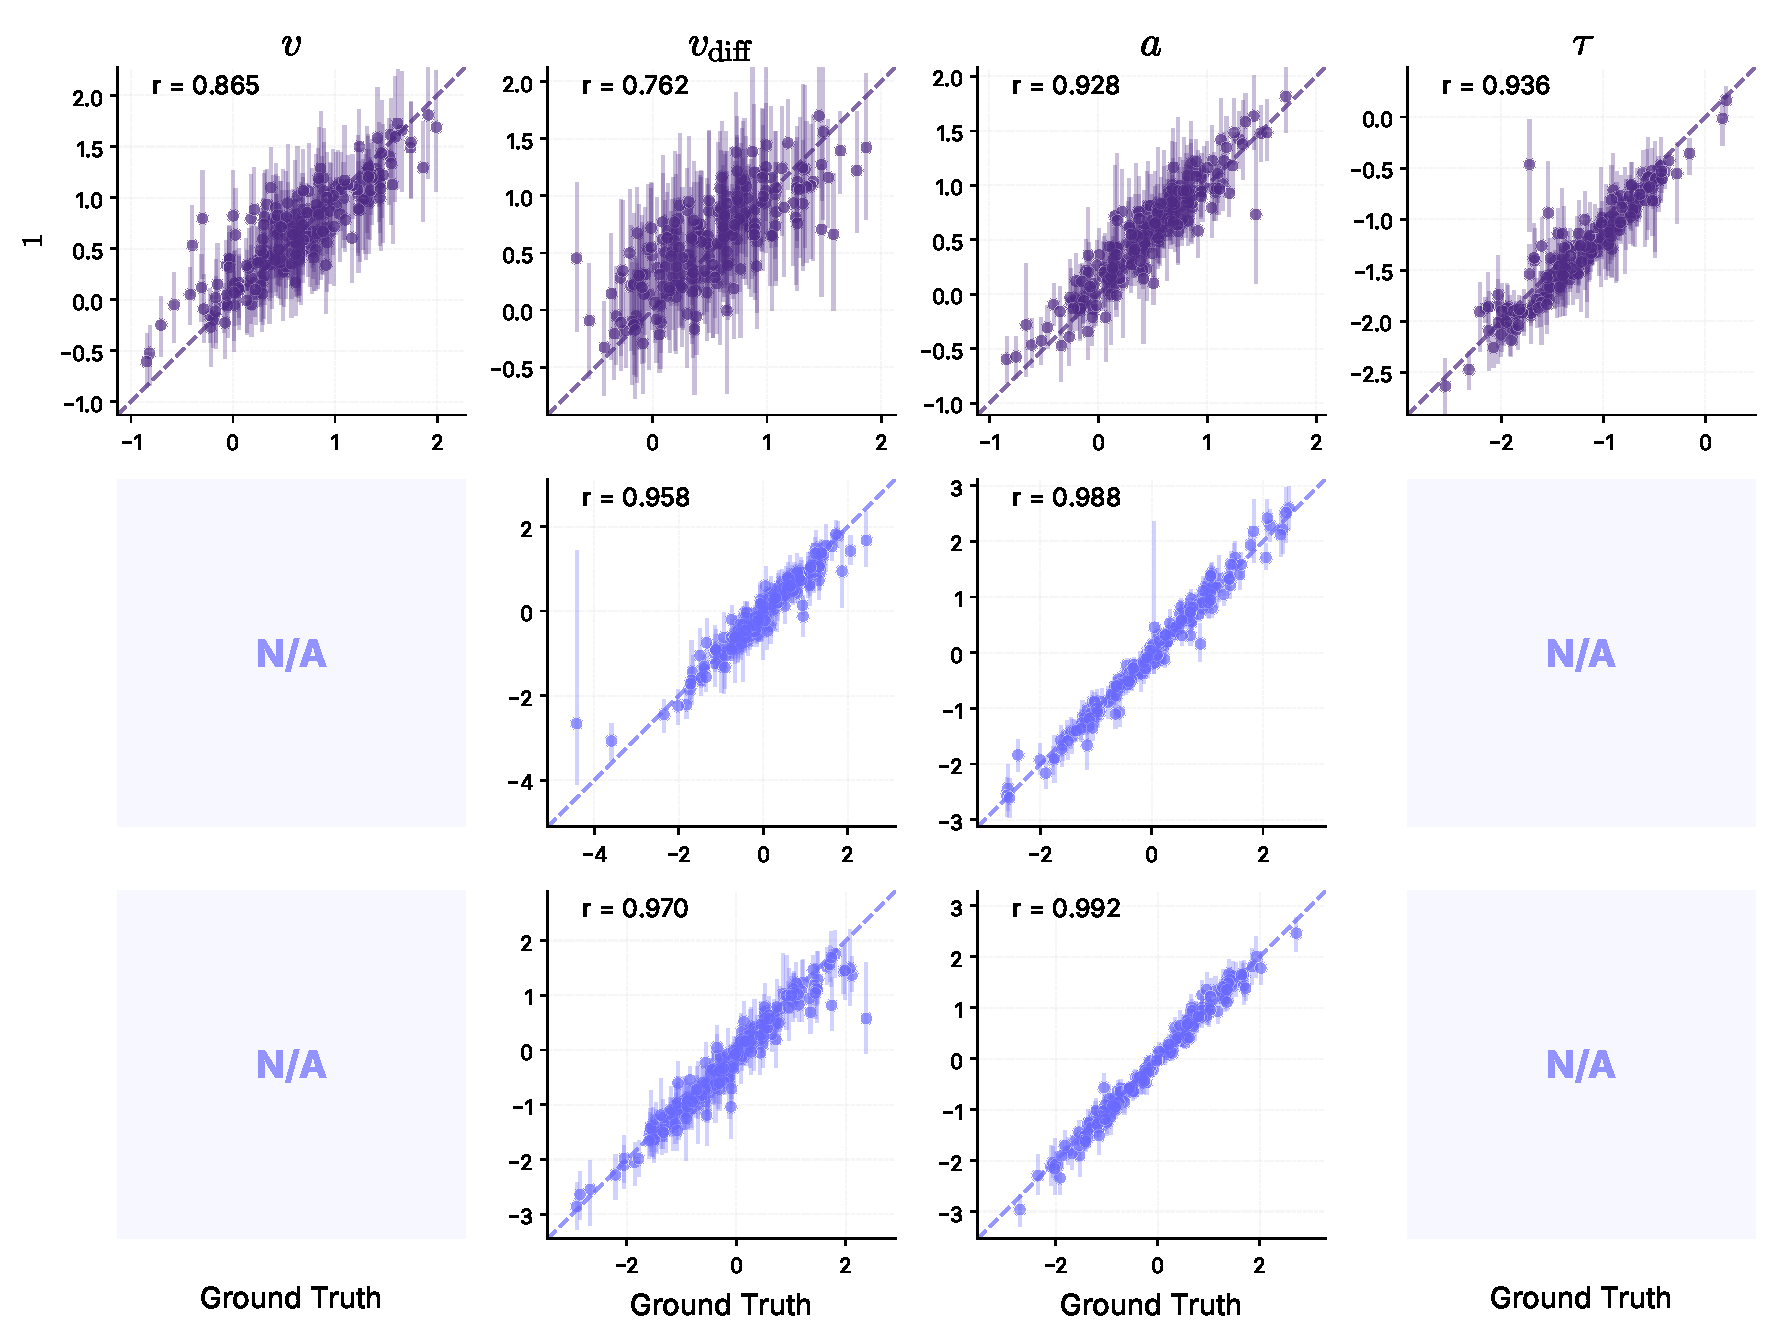
\includegraphics[width=\textwidth,height=0.3\textheight,keepaspectratio]{finetuned/lba/fixed_regressed/recovery.pdf}
    \caption{Recovery}
  \end{subfigure}\\[1ex]
  \begin{subfigure}{\textwidth}\centering
    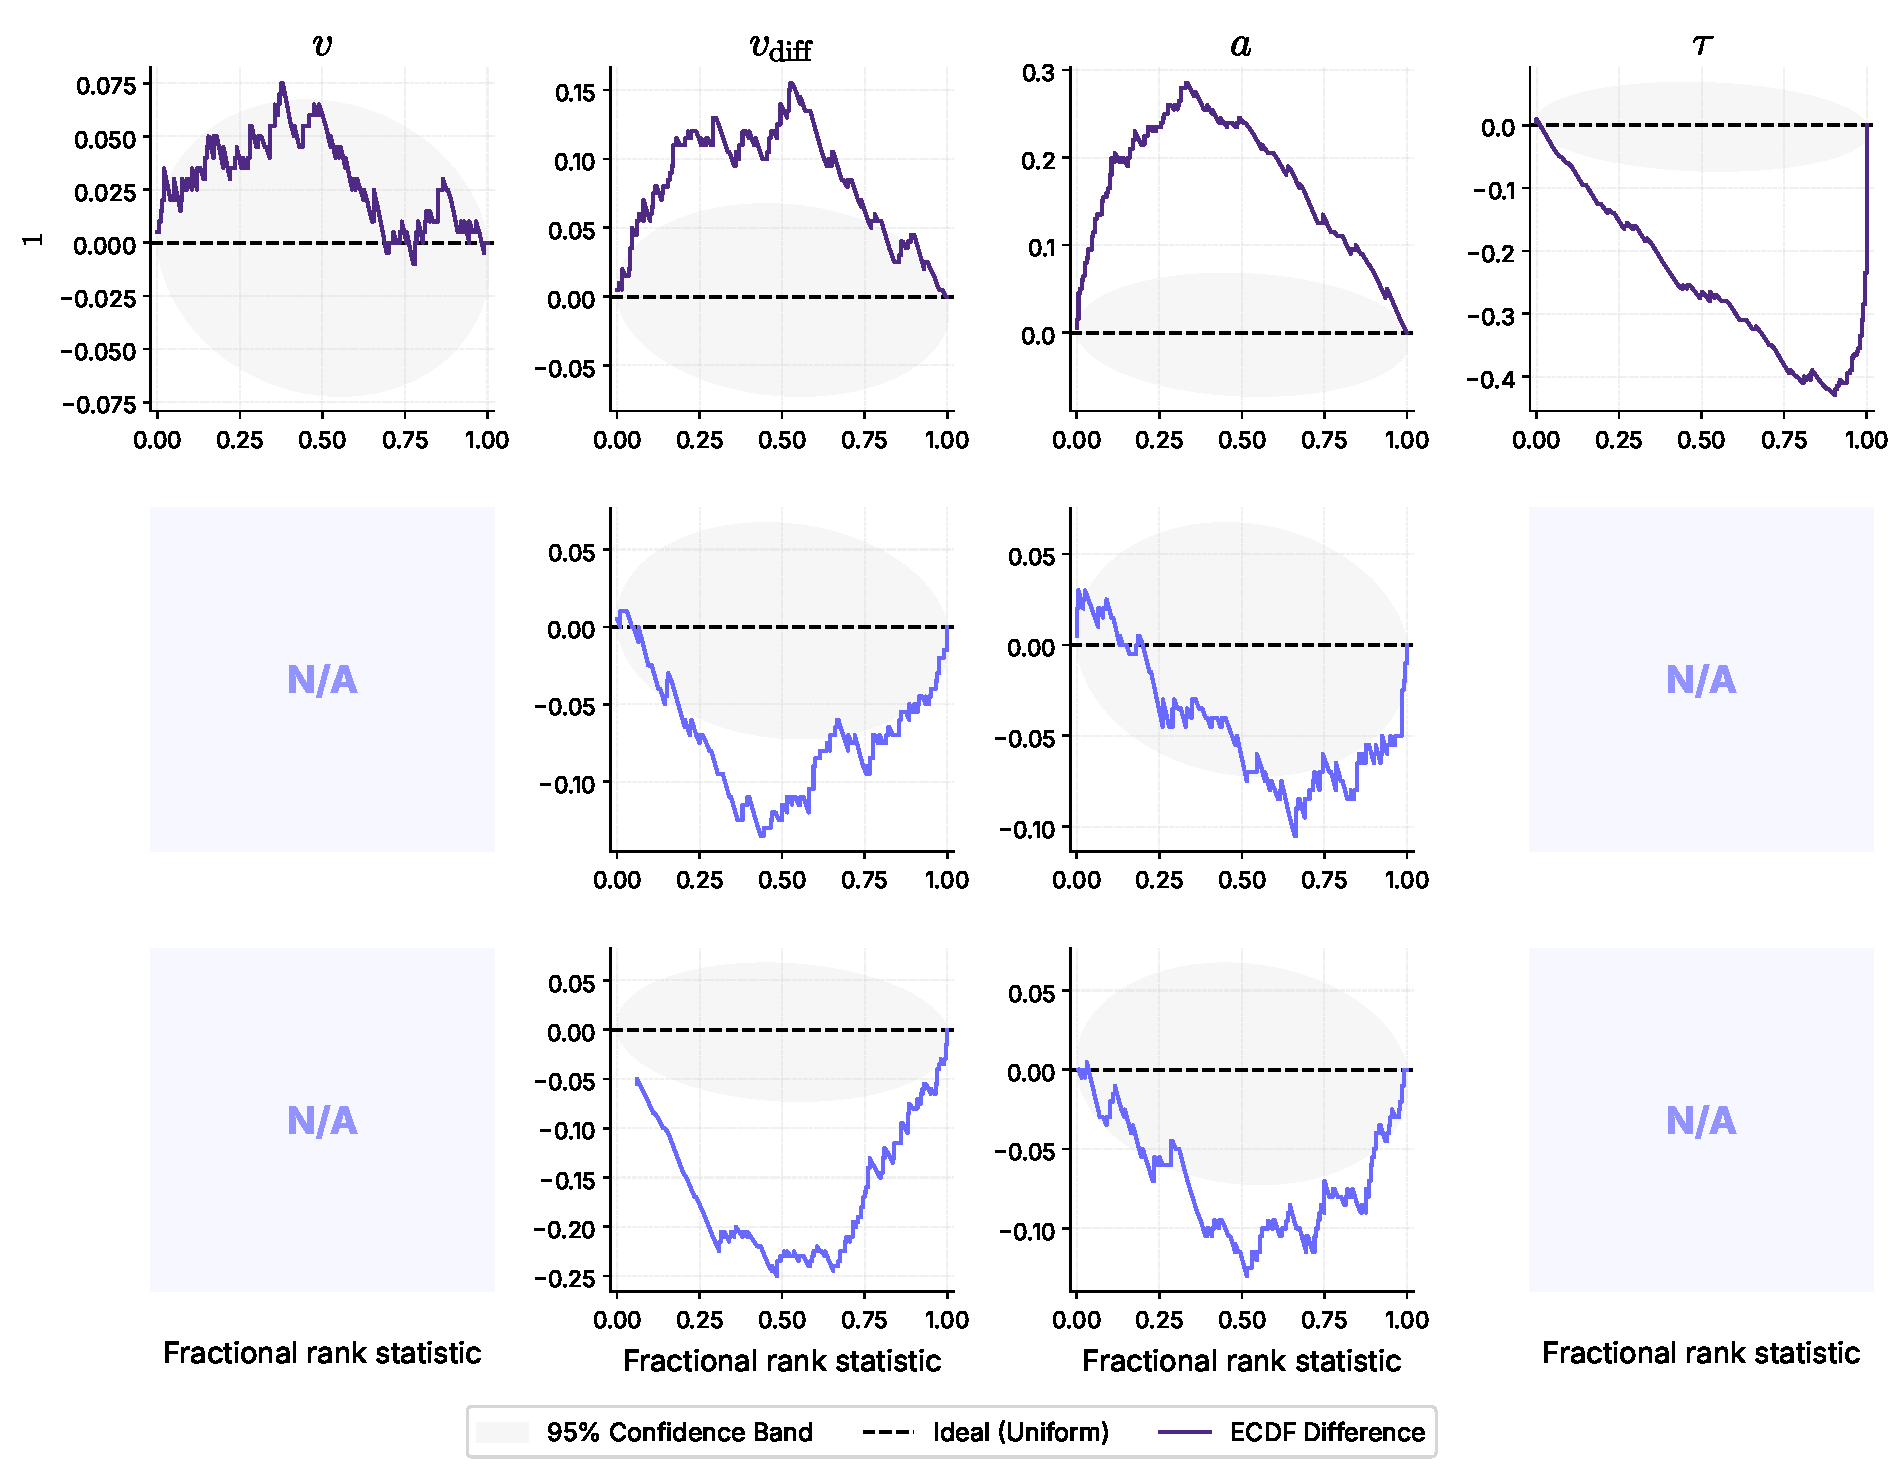
\includegraphics[width=\textwidth,height=0.3\textheight,keepaspectratio]{finetuned/lba/fixed_regressed/ecdf.pdf}
    \caption{Calibration (ECDF)}
  \end{subfigure}\\[1ex]
  \begin{subfigure}{\textwidth}\centering
    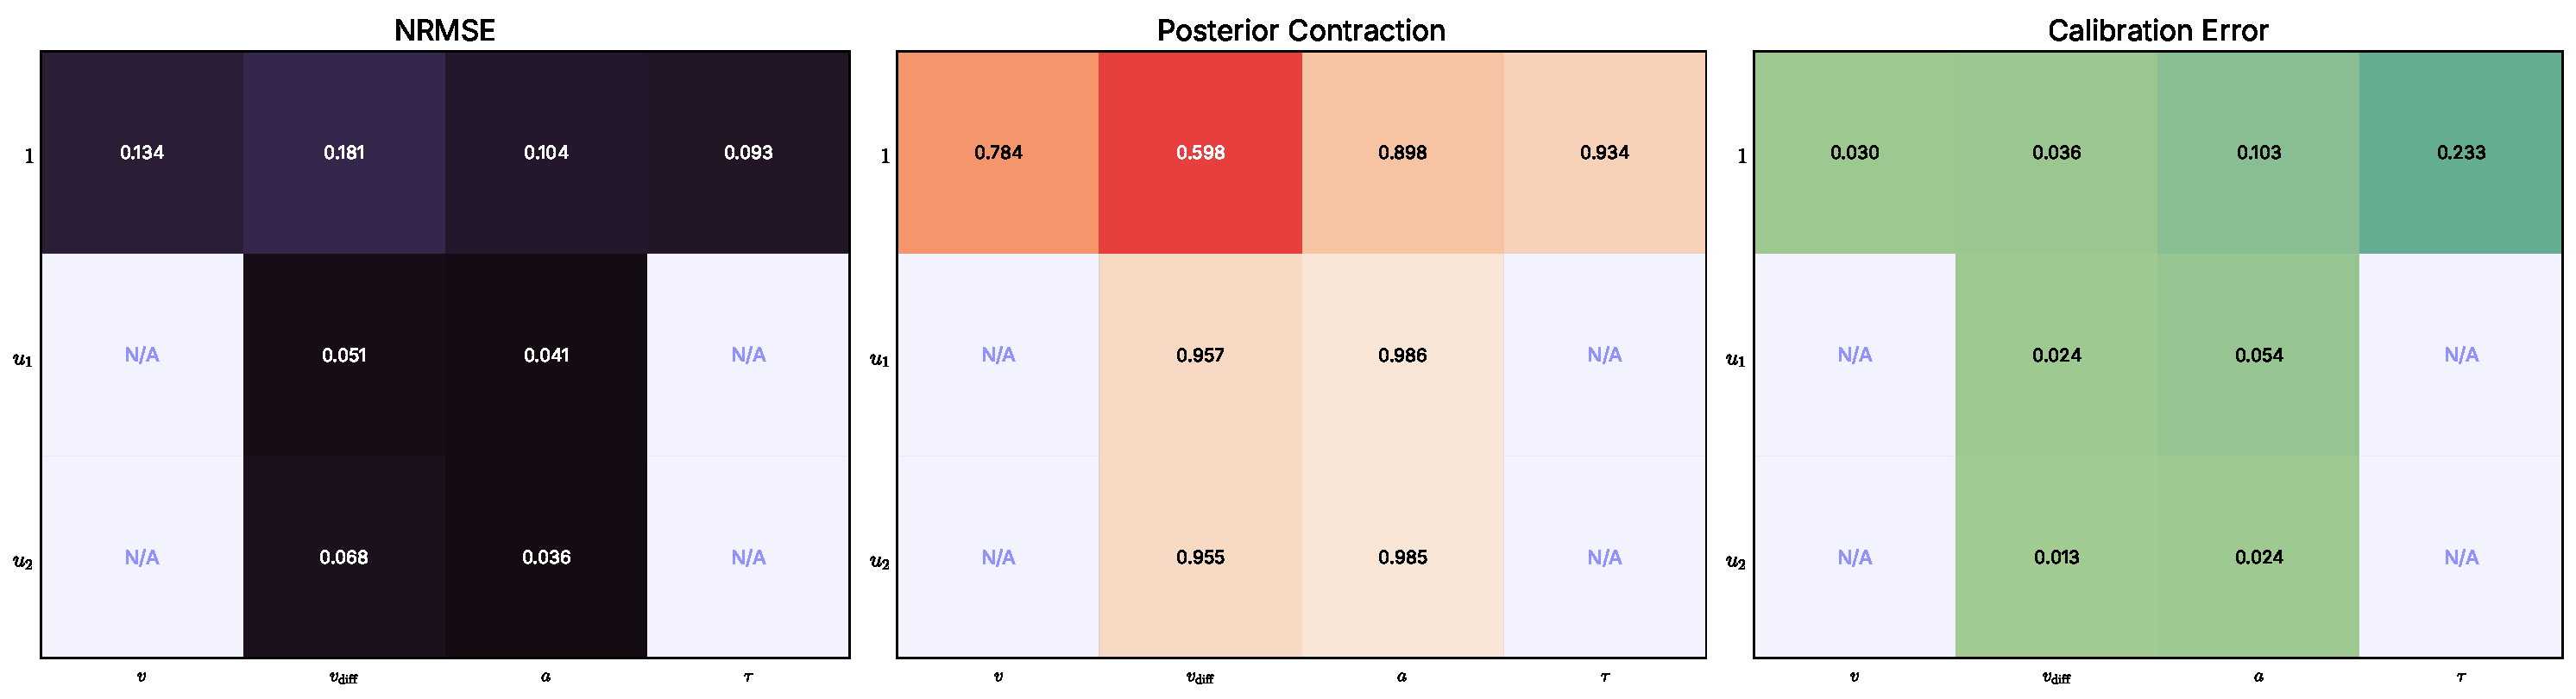
\includegraphics[width=\textwidth]{finetuned/lba/fixed_regressed/metrics.pdf}
    \caption{Metrics}
  \end{subfigure}
  \caption{\textbf{After fine-tuning: LBA, \emph{fixed + regressed} design.} (a) Recovery, (b) calibration, (c) metrics. $s_v$ and $s_\tau$ are fixed at 0 and not estimated; $v_{\mathrm{diff}}$ and $a$ carry slopes on $u_1$ and $u_2$ (8 coefficients shown). As in Figure~\ref{fig:app3-finetuned-lba-intercept-only}; zero-shot counterpart: Figure~\ref{fig:app3-zeroshot-lba-fixed-regressed}.}
  \label{fig:app3-finetuned-lba-fixed-regressed}
\end{figure}

\begin{figure}[p]
  \centering
  \begin{subfigure}{\textwidth}\centering
    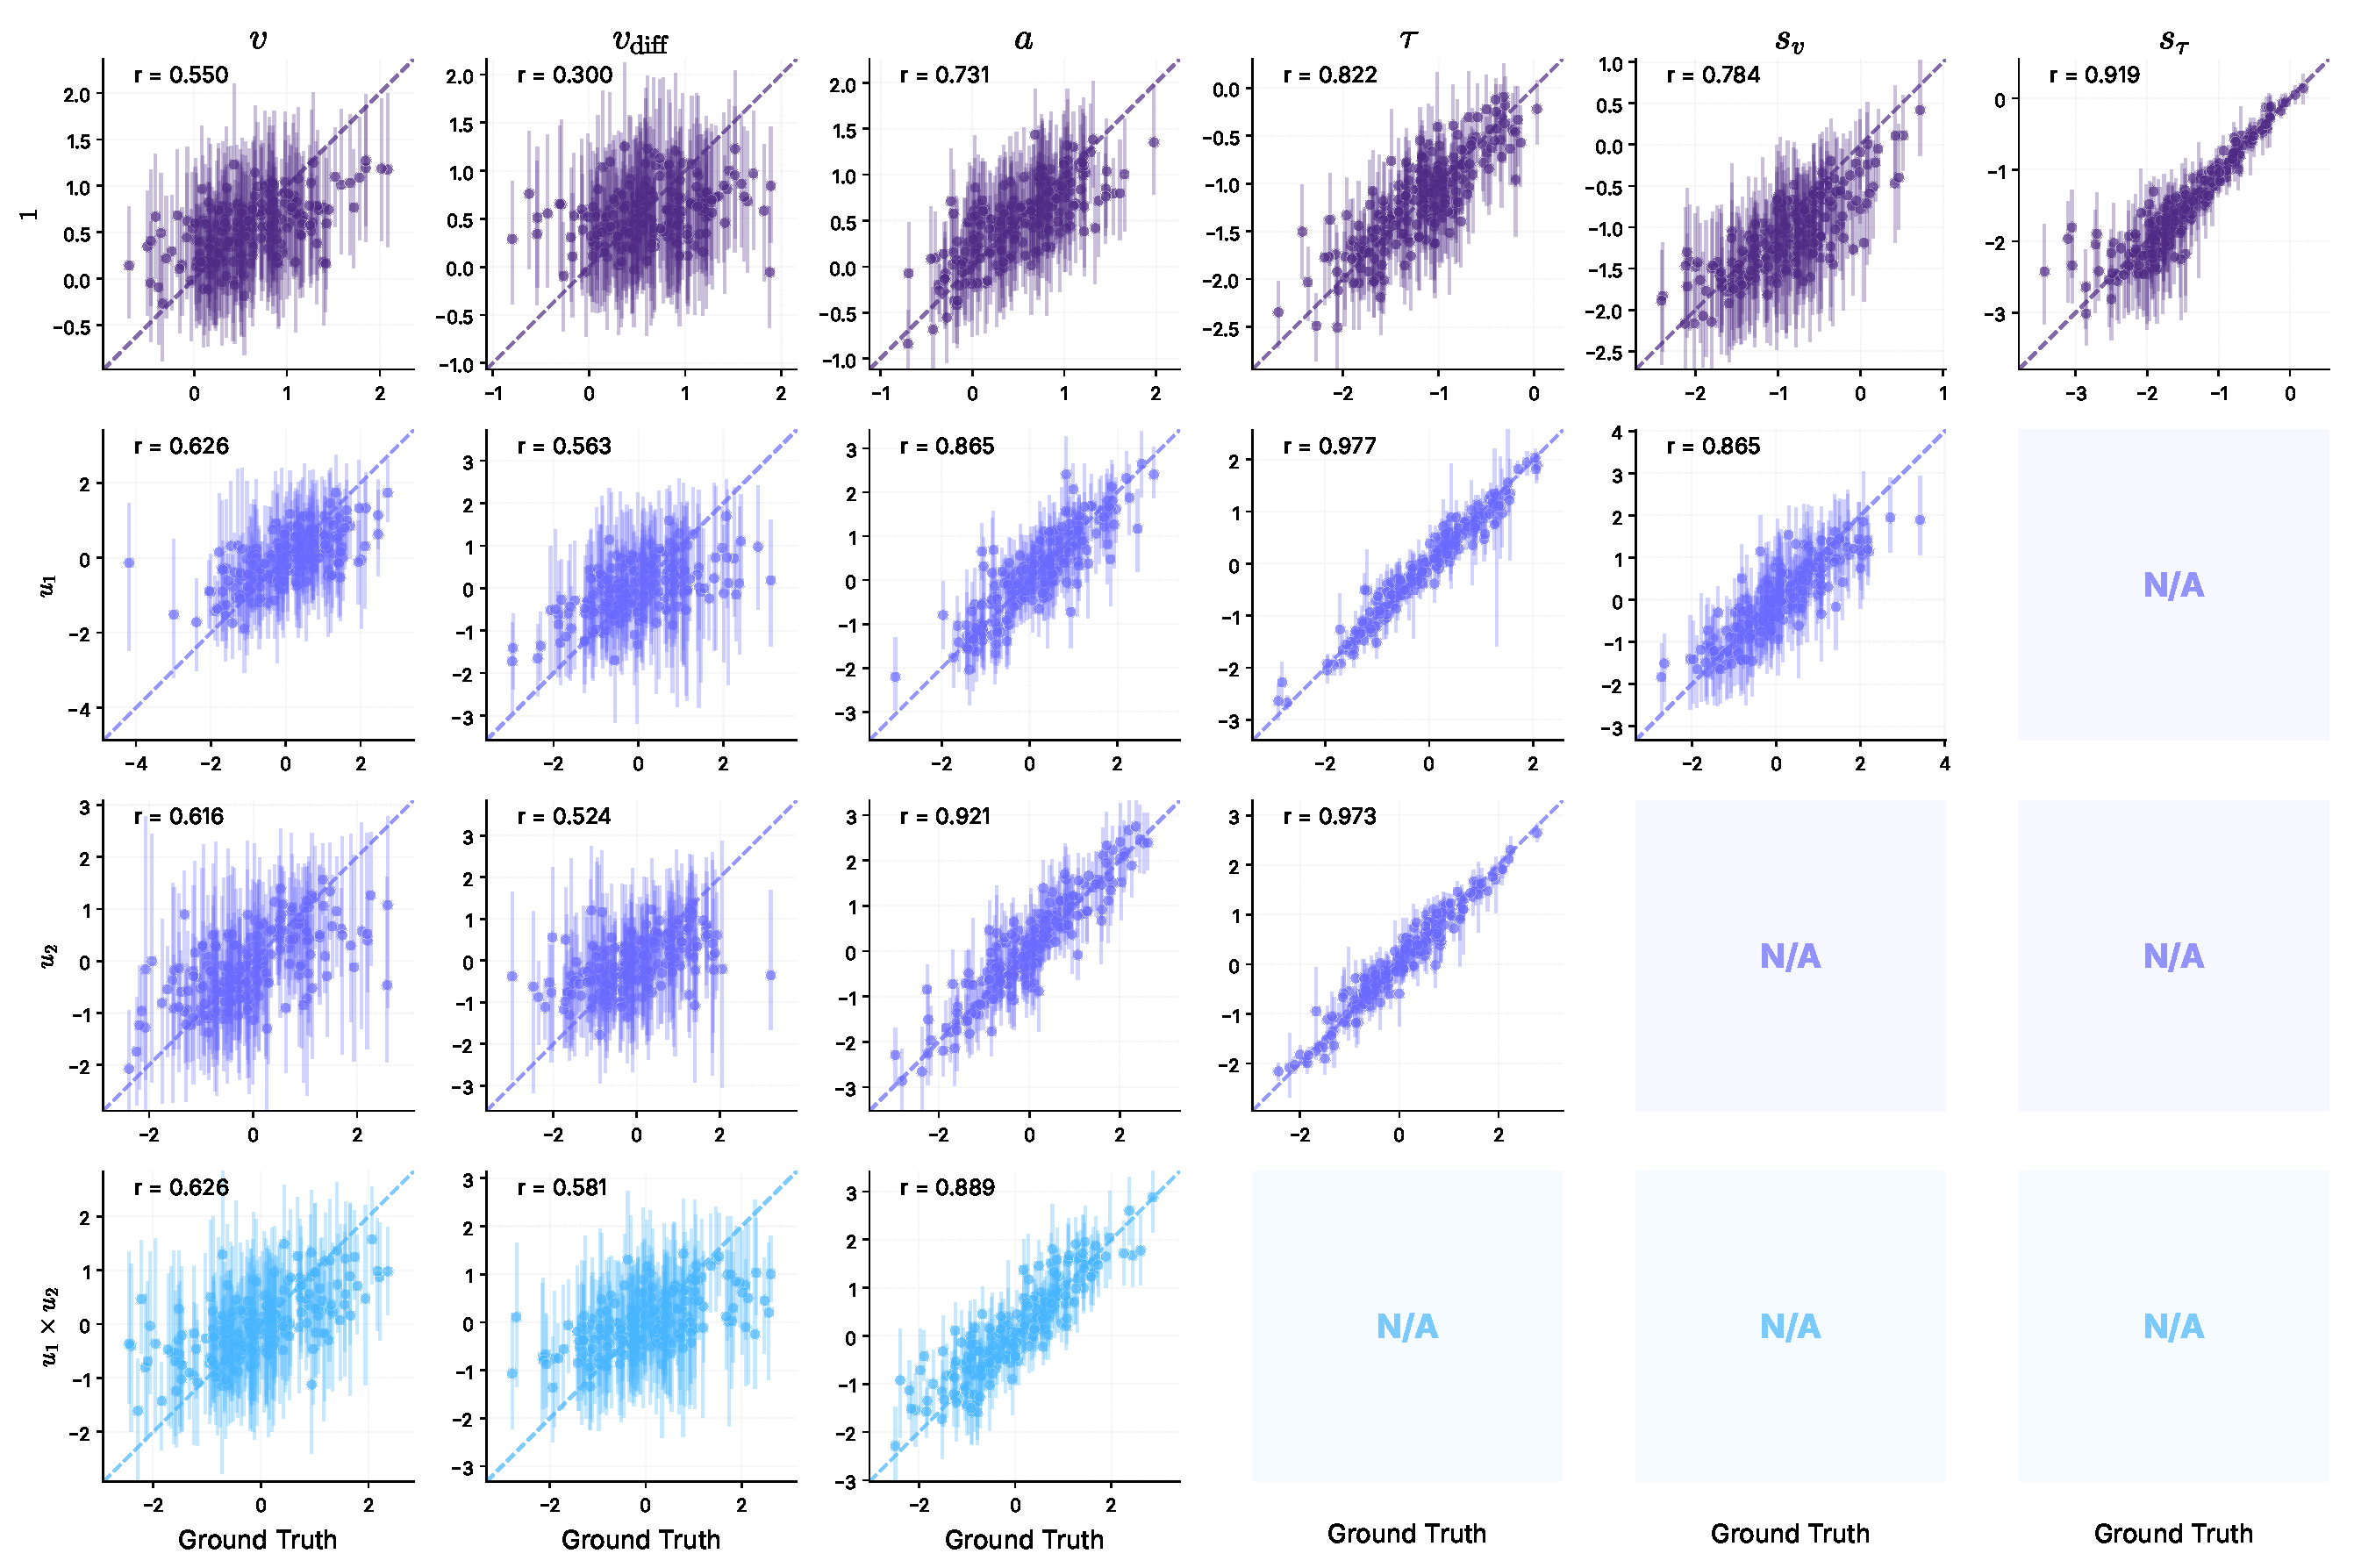
\includegraphics[width=\textwidth,height=0.3\textheight,keepaspectratio]{finetuned/lba/interaction/recovery.pdf}
    \caption{Recovery}
  \end{subfigure}\\[1ex]
  \begin{subfigure}{\textwidth}\centering
    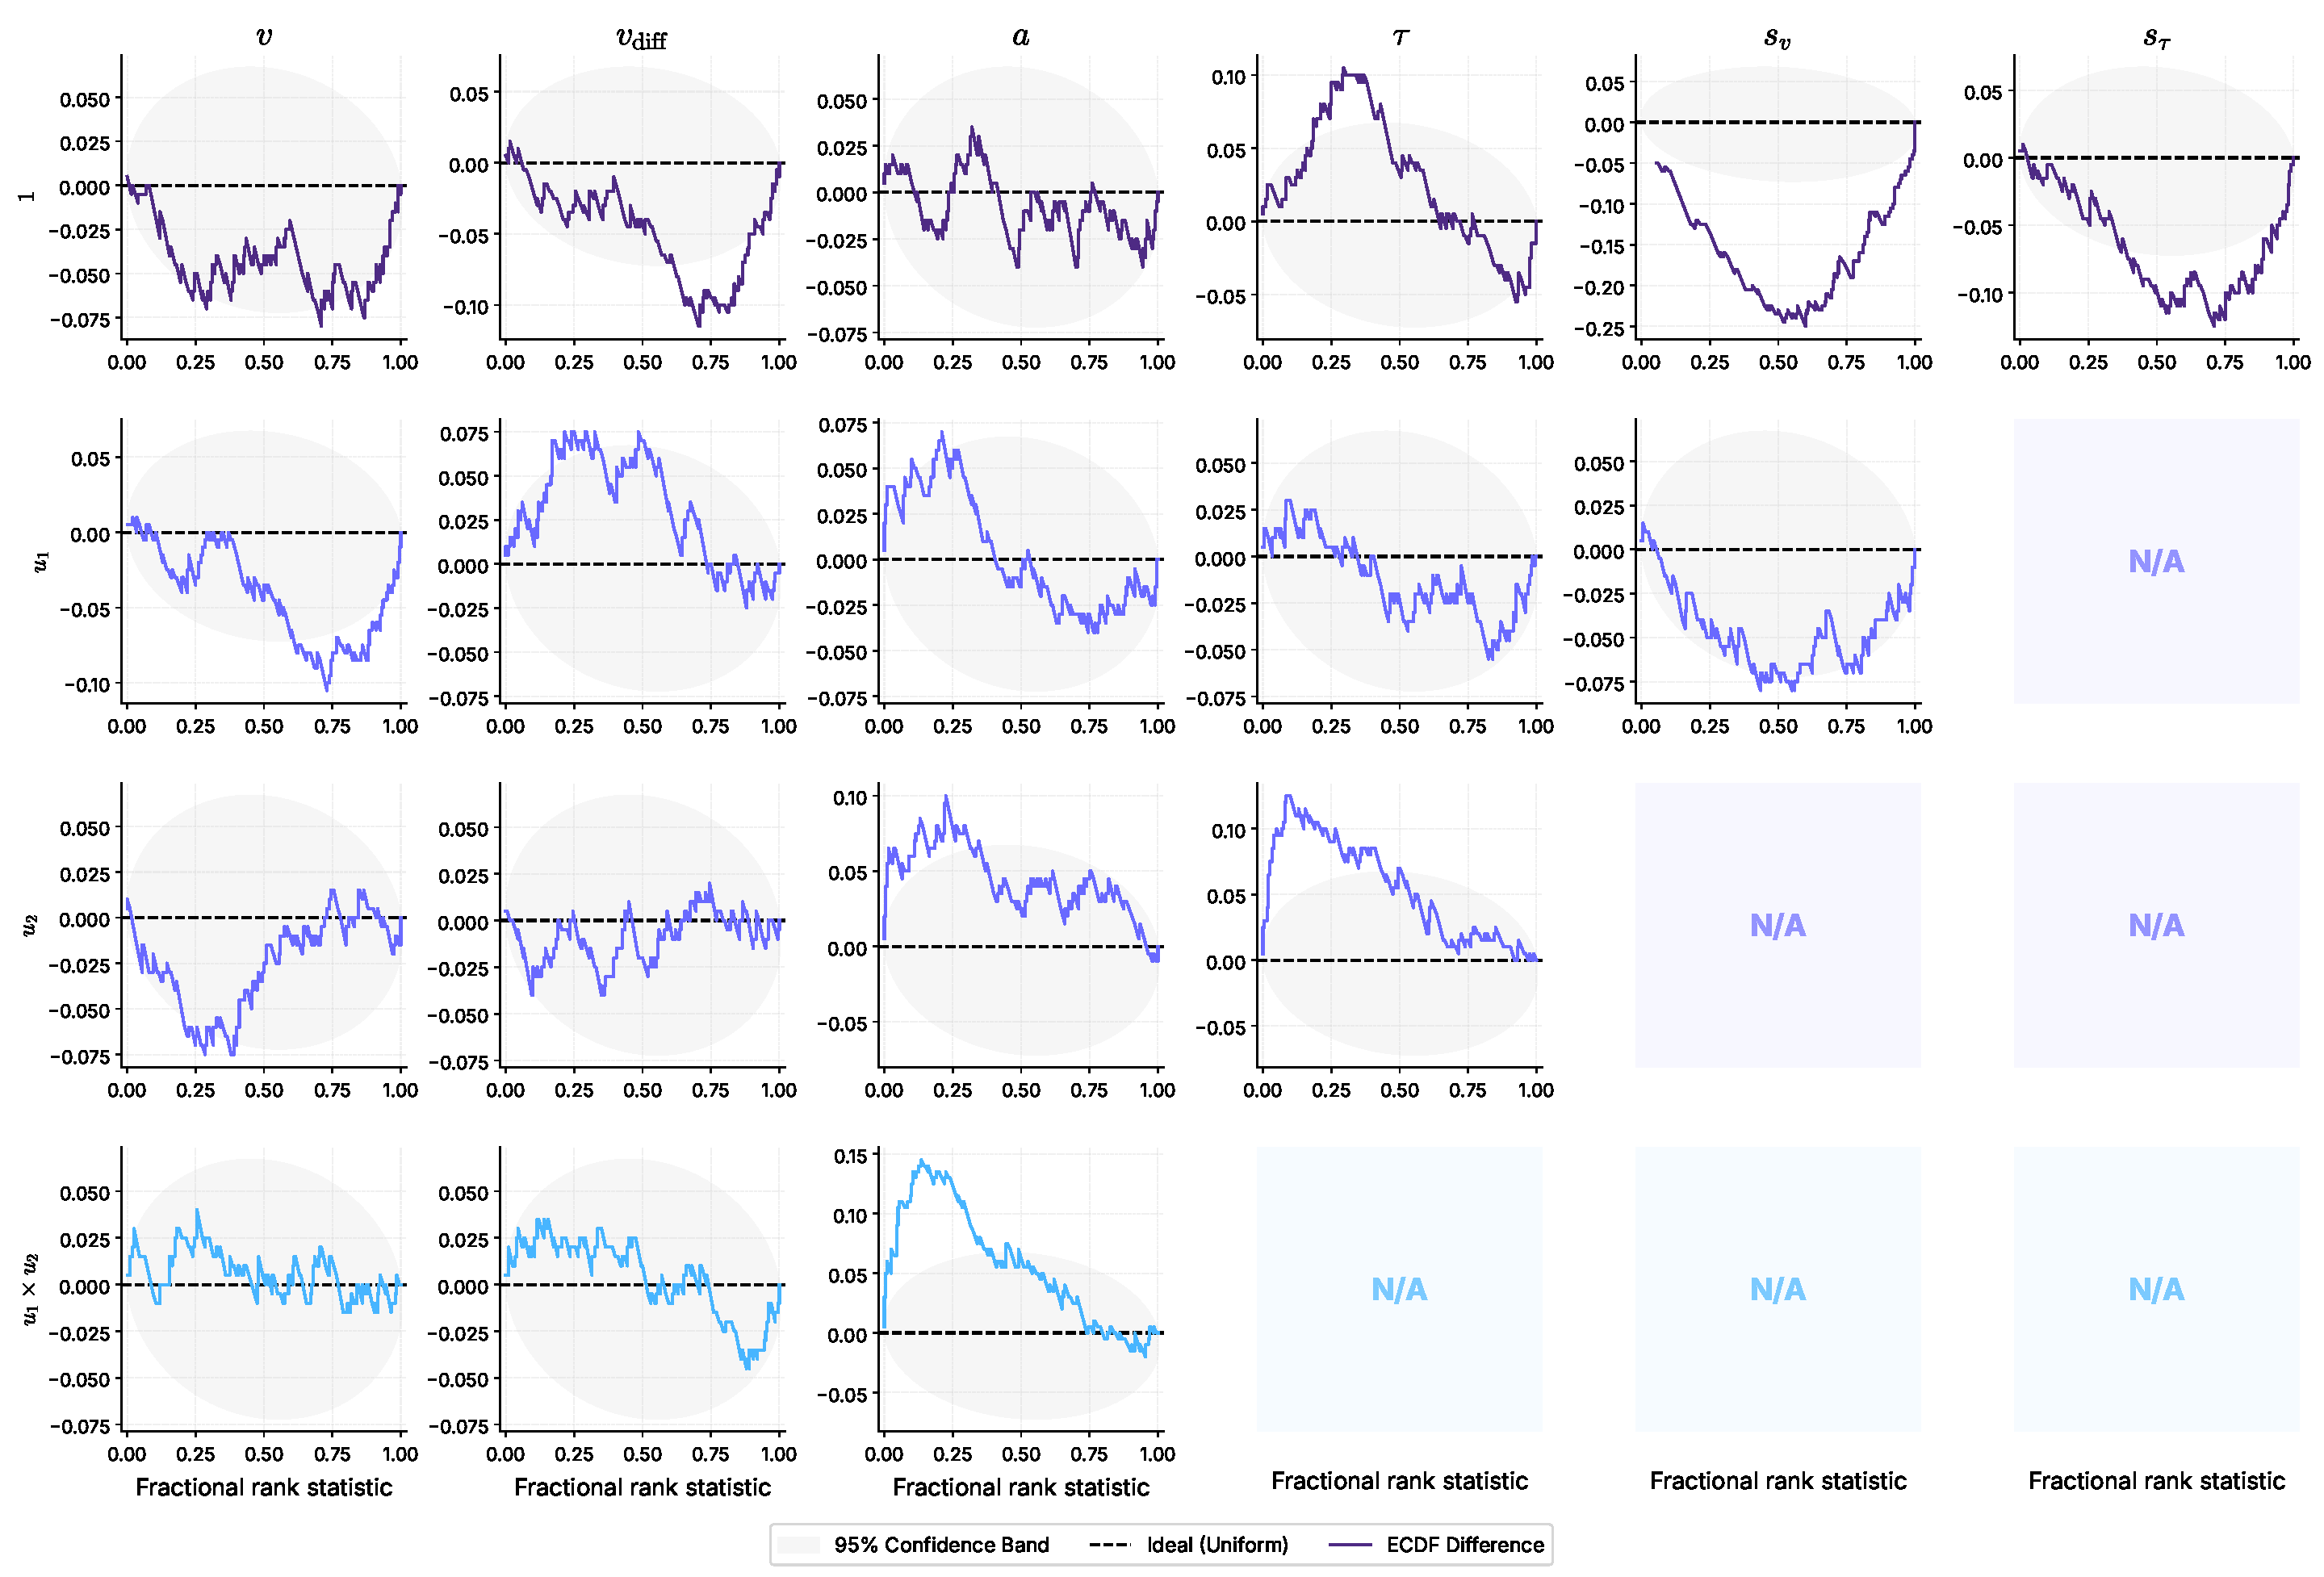
\includegraphics[width=\textwidth,height=0.3\textheight,keepaspectratio]{finetuned/lba/interaction/ecdf.pdf}
    \caption{Calibration (ECDF)}
  \end{subfigure}\\[1ex]
  \begin{subfigure}{\textwidth}\centering
    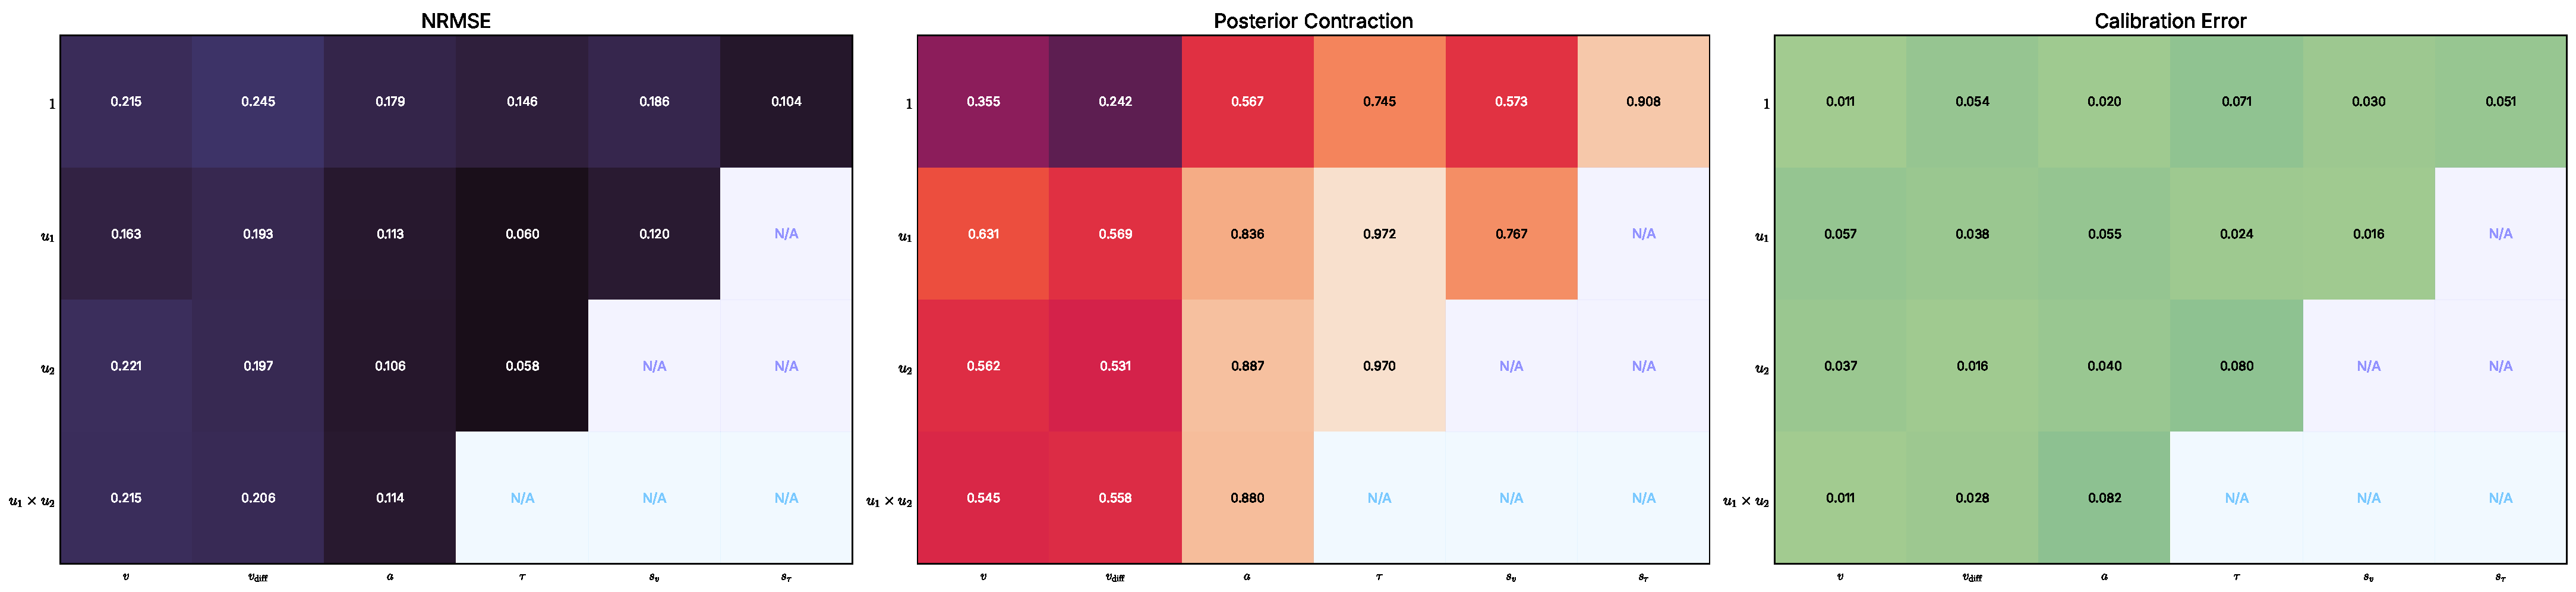
\includegraphics[width=\textwidth]{finetuned/lba/interaction/metrics.pdf}
    \caption{Metrics}
  \end{subfigure}
  \caption{\textbf{After fine-tuning: LBA, \emph{interaction} design.} (a) Recovery, (b) calibration, (c) metrics. $v$, $v_{\mathrm{diff}}$, $a$, $\tau$ and $s_v$ carry slopes on $u_1$; $v$, $v_{\mathrm{diff}}$, $a$ and $\tau$ carry slopes on $u_2$; $v$, $v_{\mathrm{diff}}$ and $a$ on the product $u_1 u_2$ (18 coefficients shown). As in Figure~\ref{fig:app3-finetuned-lba-intercept-only}; zero-shot counterpart: Figure~\ref{fig:app3-zeroshot-lba-interaction}.}
  \label{fig:app3-finetuned-lba-interaction}
\end{figure}

\begin{figure}[p]
  \centering
  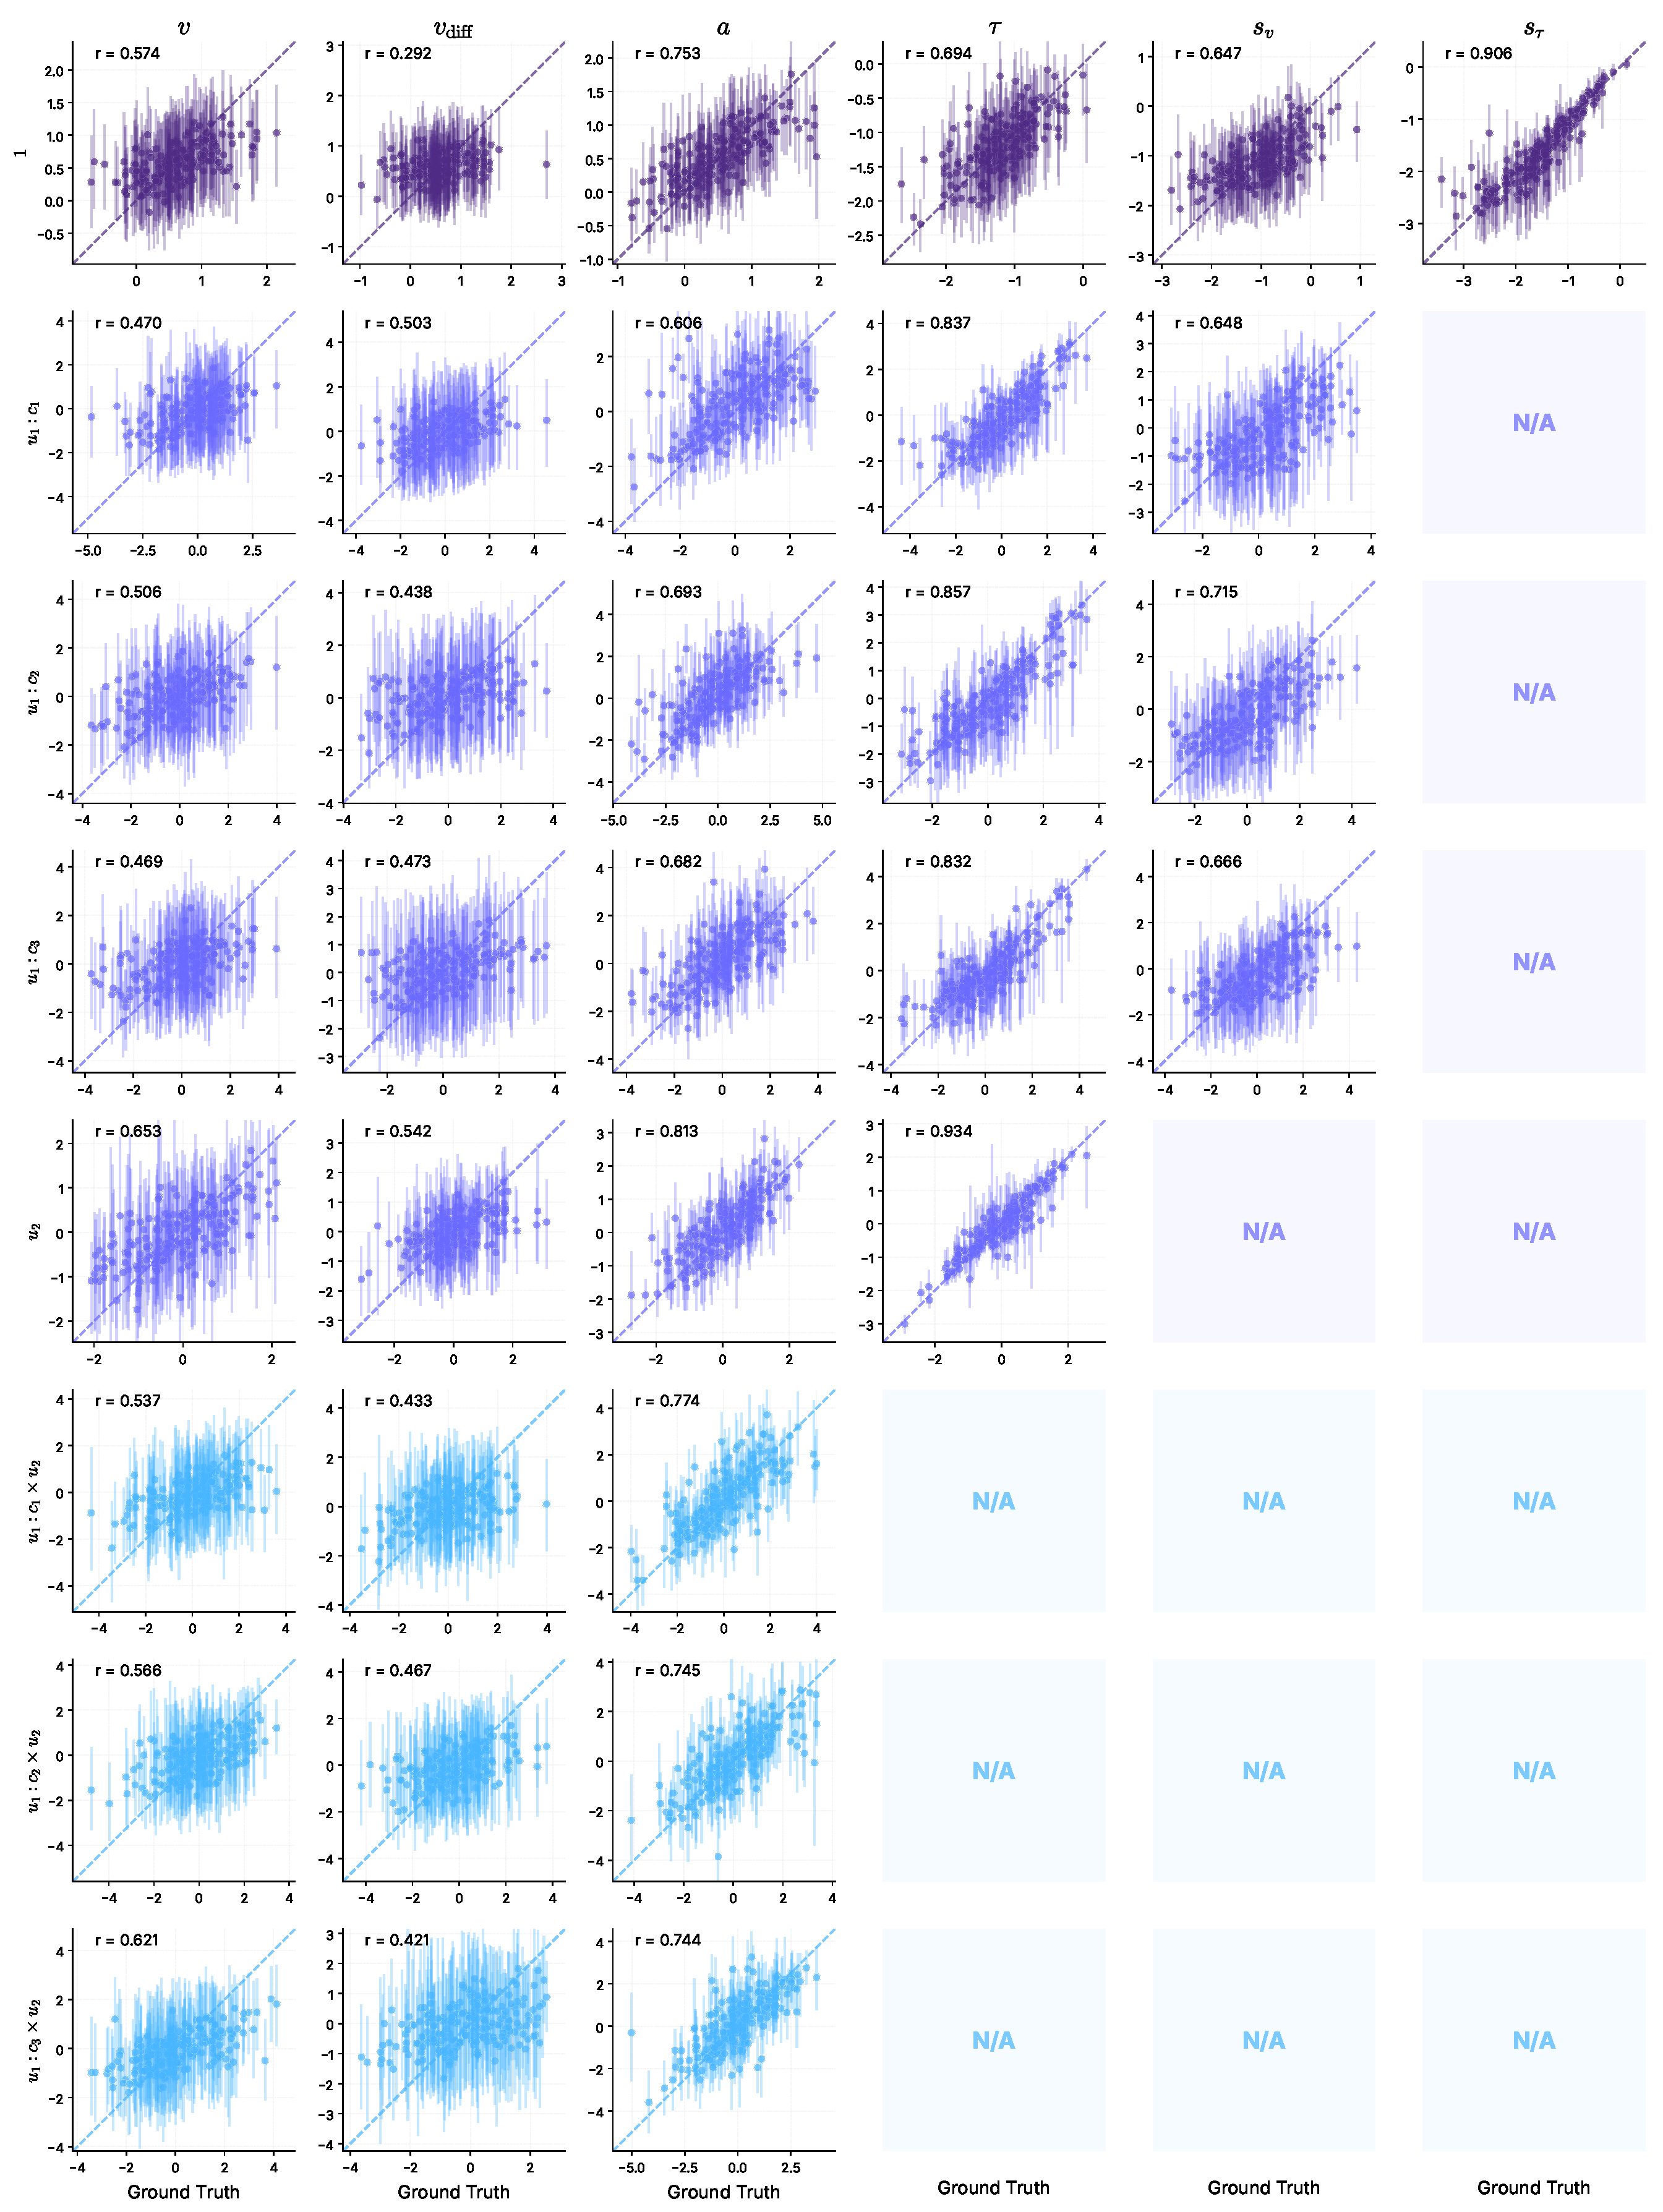
\includegraphics[width=\textwidth,height=0.82\textheight,keepaspectratio]{finetuned/lba/mixed_predictor/recovery.pdf}
  \caption{\textbf{Parameter recovery, LBA after fine-tuning, mixed-predictor design.} $v$, $v_{\mathrm{diff}}$, $a$, $\tau$ and $s_v$ carry effects of the four-level $u_1$; $v$, $v_{\mathrm{diff}}$, $a$ and $\tau$ slopes on $u_2$; $v$, $v_{\mathrm{diff}}$ and $a$ the interaction (34 coefficients shown). Datasets simulated for this design (no shared benchmark file exists); design as in Figure~\ref{fig:app1-ddm-mixed-predictor-recovery}, encoding as in the top panel of Figure~\ref{fig:app1-ddm-intercept-only-cf}.}
  \label{fig:app3-finetuned-lba-mixed-predictor-recovery}
\end{figure}

\begin{figure}[p]
  \centering
  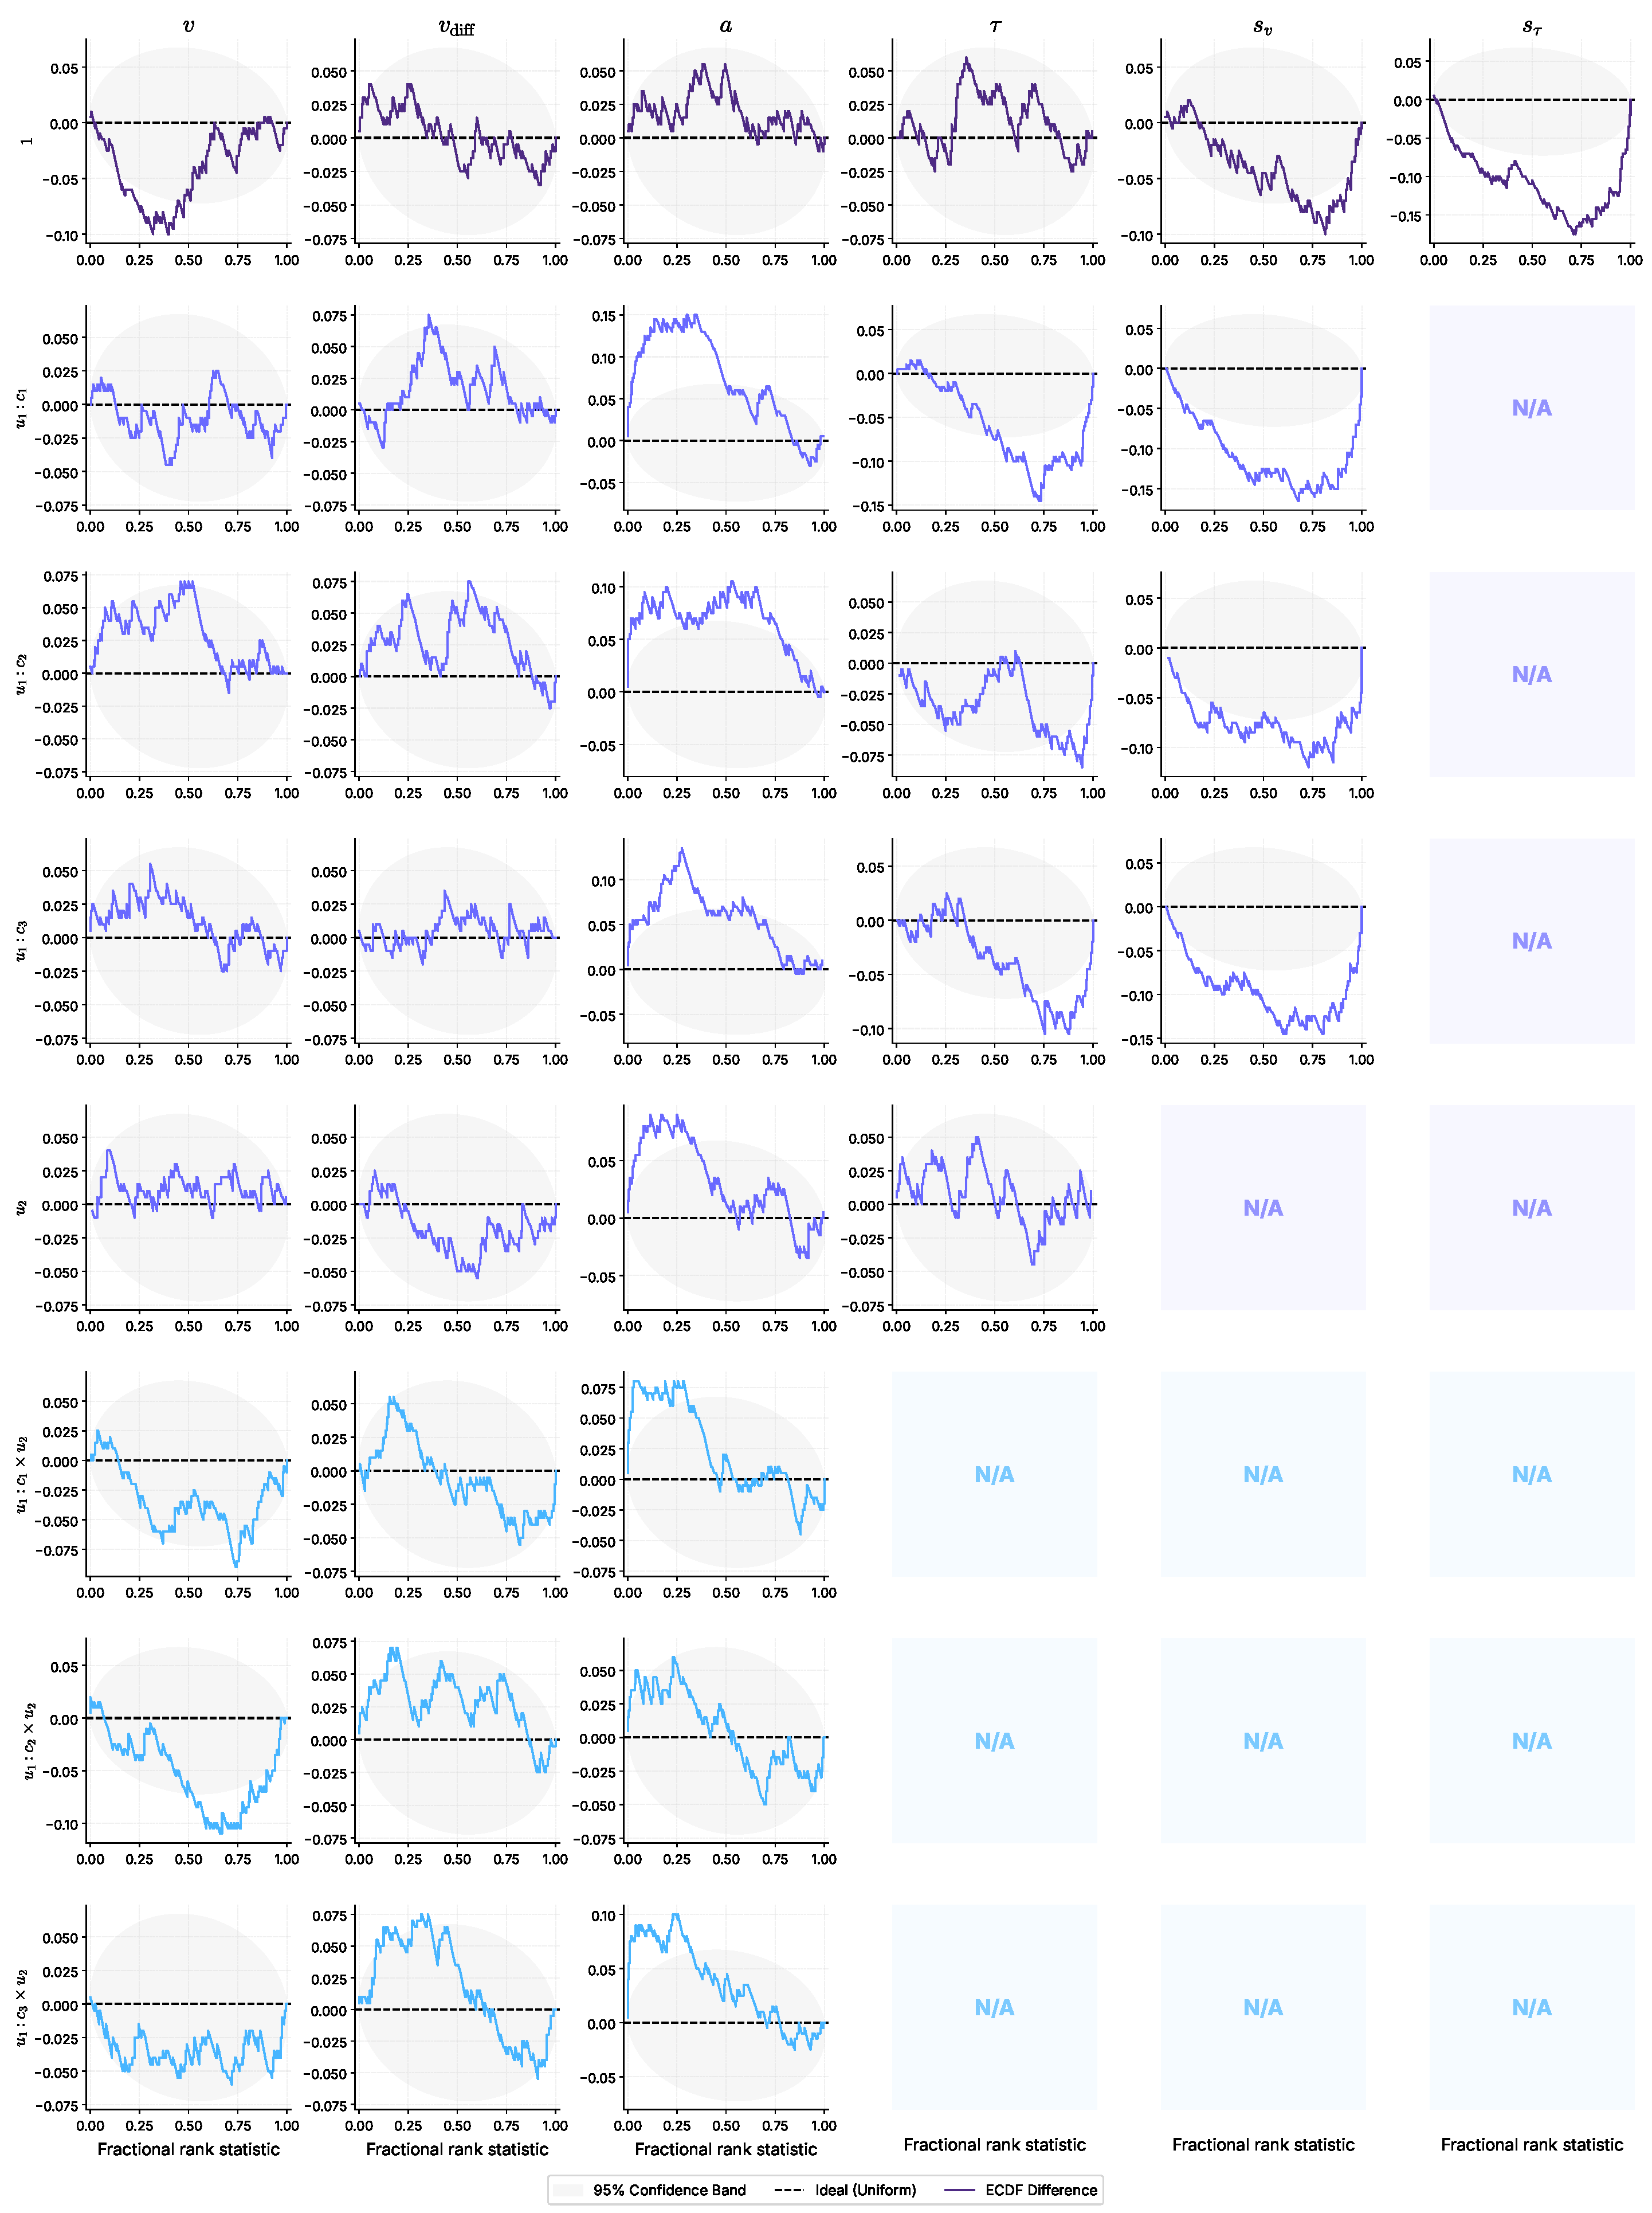
\includegraphics[width=\textwidth,height=0.82\textheight,keepaspectratio]{finetuned/lba/mixed_predictor/ecdf.pdf}
  \caption{\textbf{Simulation-based calibration, LBA after fine-tuning, mixed-predictor design.} $v$, $v_{\mathrm{diff}}$, $a$, $\tau$ and $s_v$ carry effects of the four-level $u_1$; $v$, $v_{\mathrm{diff}}$, $a$ and $\tau$ slopes on $u_2$; $v$, $v_{\mathrm{diff}}$ and $a$ the interaction (34 coefficients shown). Datasets simulated for this design (no shared benchmark file exists); design as in Figure~\ref{fig:app1-ddm-mixed-predictor-recovery}, encoding as in the middle panel of Figure~\ref{fig:app1-ddm-intercept-only-cf}.}
  \label{fig:app3-finetuned-lba-mixed-predictor-ecdf}
\end{figure}

\begin{figure}[p]
  \centering
  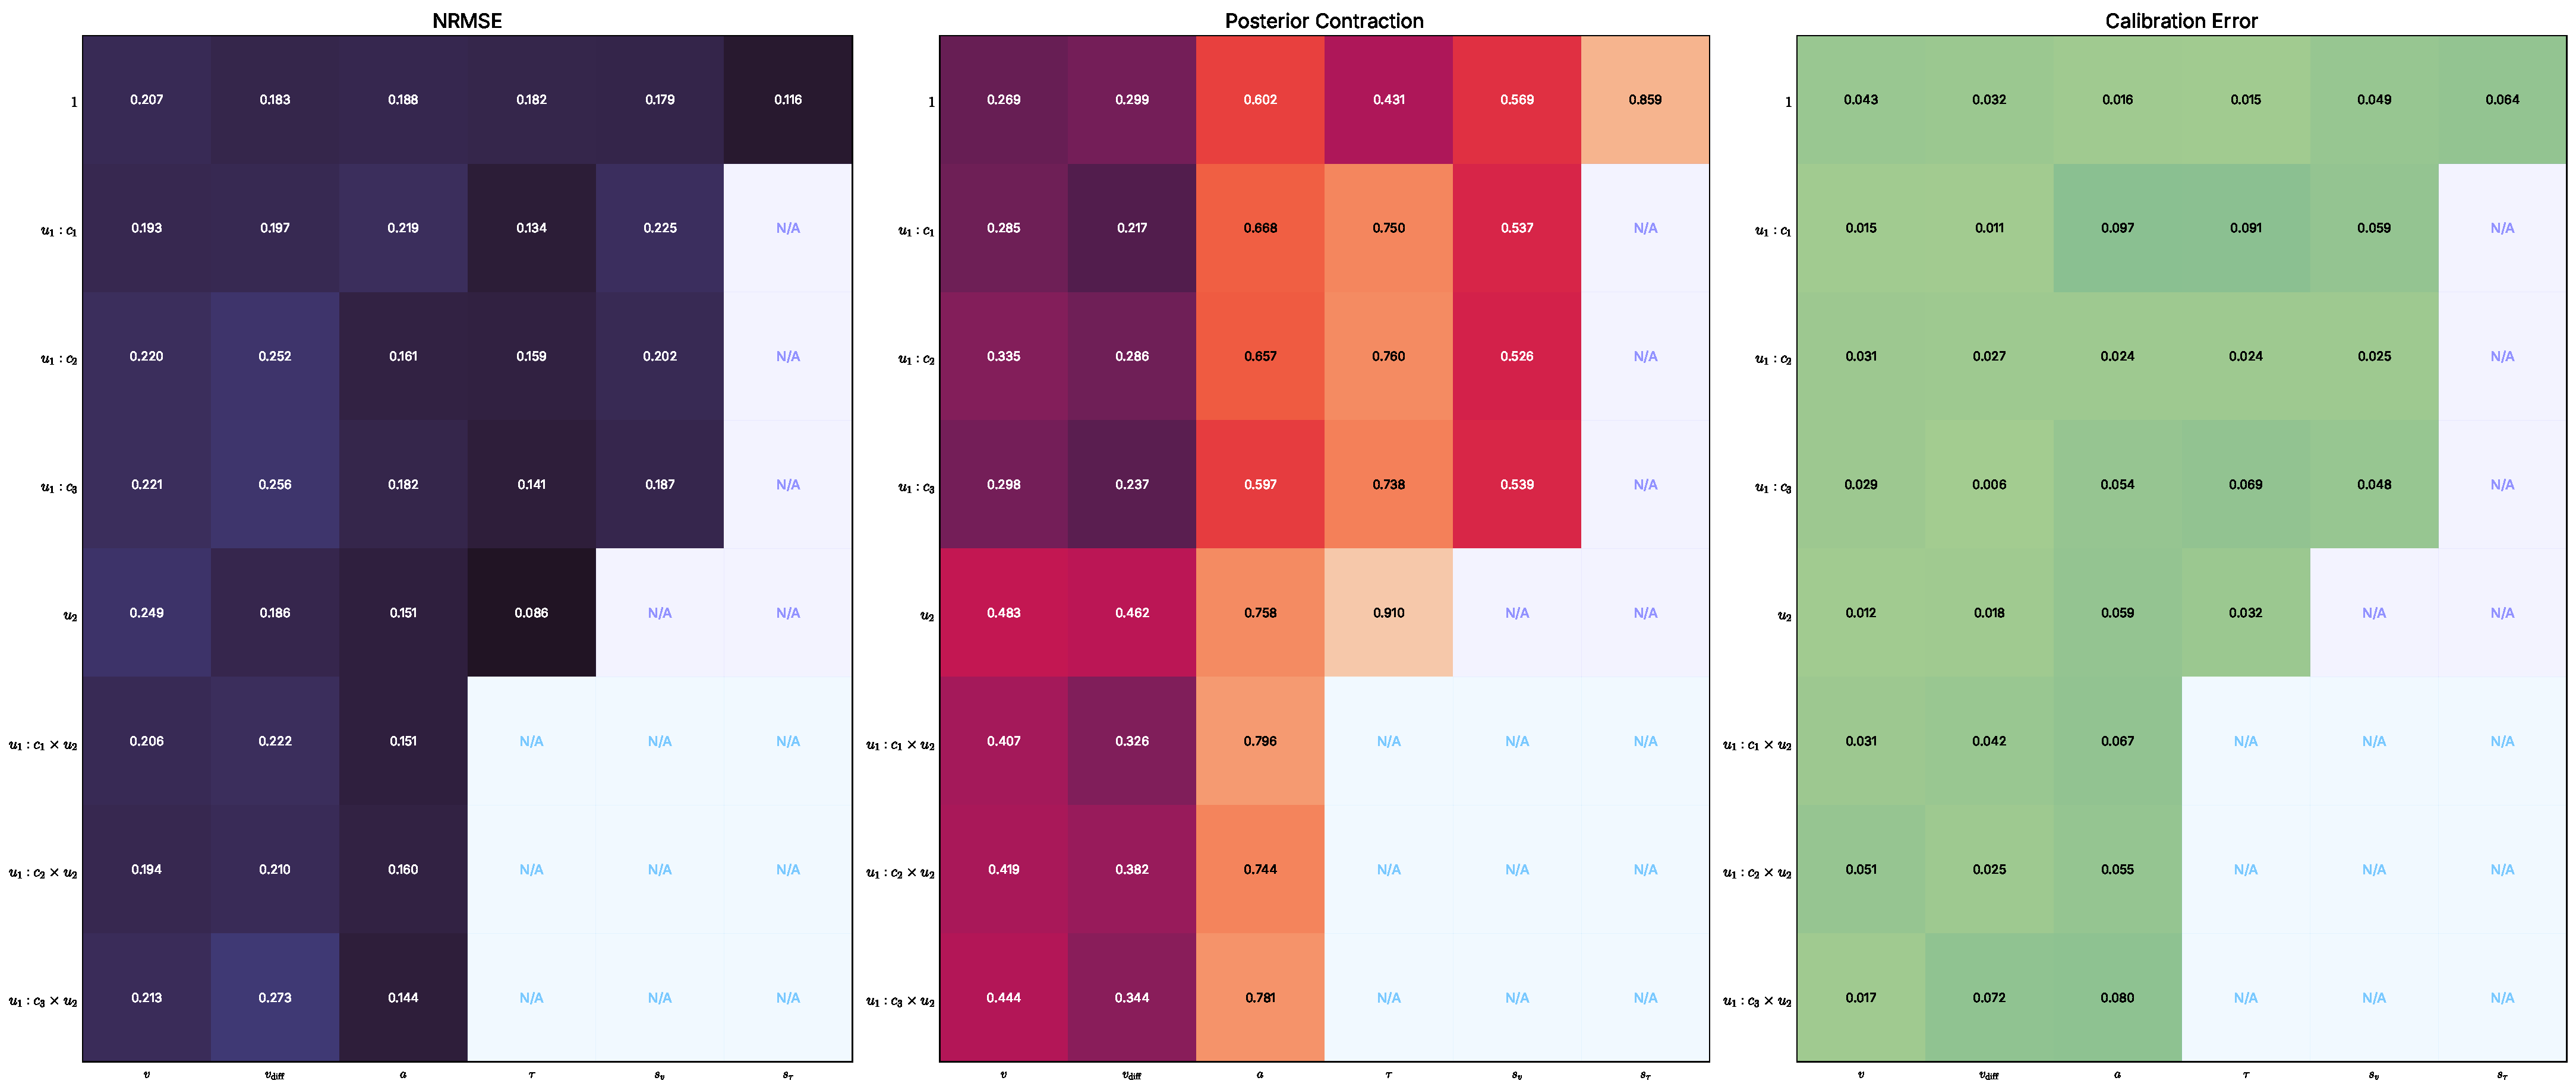
\includegraphics[width=\textwidth,height=0.82\textheight,keepaspectratio]{finetuned/lba/mixed_predictor/metrics.pdf}
  \caption{\textbf{Summary metrics, LBA after fine-tuning, mixed-predictor design.} $v$, $v_{\mathrm{diff}}$, $a$, $\tau$ and $s_v$ carry effects of the four-level $u_1$; $v$, $v_{\mathrm{diff}}$, $a$ and $\tau$ slopes on $u_2$; $v$, $v_{\mathrm{diff}}$ and $a$ the interaction (34 coefficients shown). Datasets simulated for this design (no shared benchmark file exists); design as in Figure~\ref{fig:app1-ddm-mixed-predictor-recovery}, encoding as in the bottom panel of Figure~\ref{fig:app1-ddm-intercept-only-cf}.}
  \label{fig:app3-finetuned-lba-mixed-predictor-metrics}
\end{figure}

\begin{figure}[p]
  \centering
  \begin{subfigure}{\textwidth}\centering
    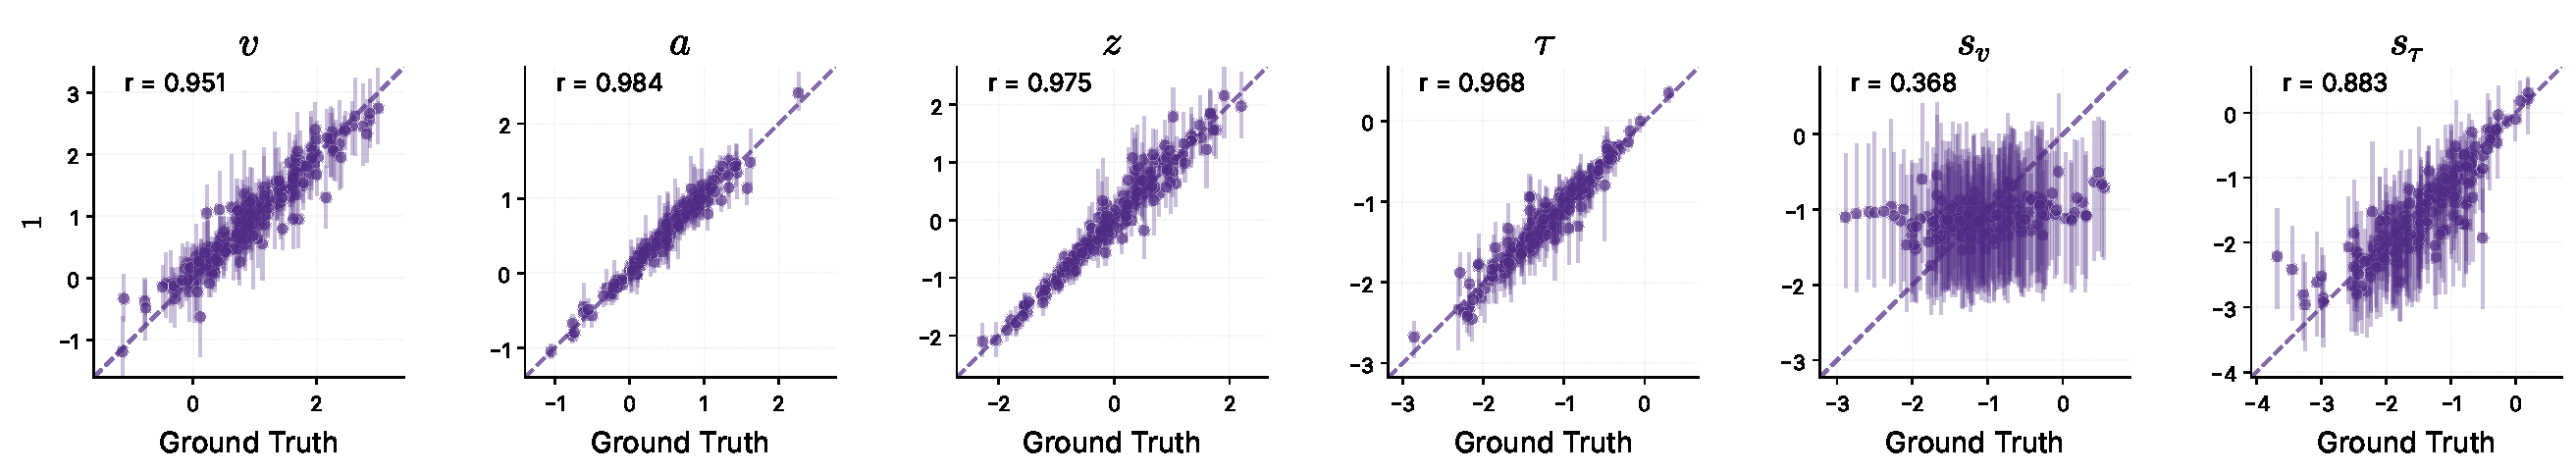
\includegraphics[width=\textwidth,height=0.3\textheight,keepaspectratio]{finetuned/ddm/intercept_only/recovery.pdf}
    \caption{Recovery}
  \end{subfigure}\\[1ex]
  \begin{subfigure}{\textwidth}\centering
    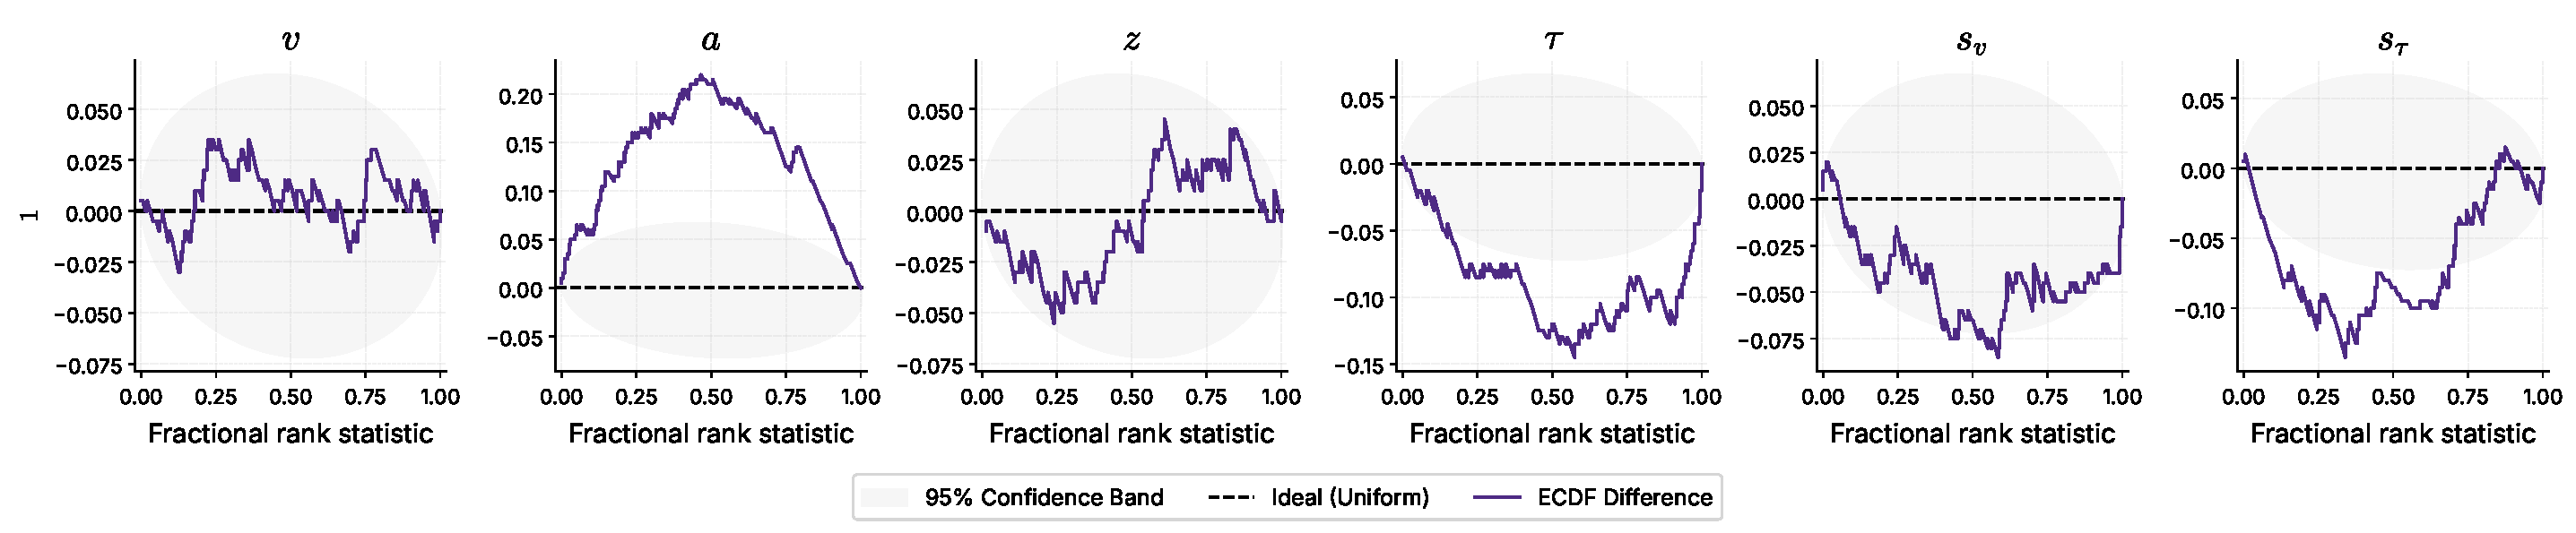
\includegraphics[width=\textwidth,height=0.3\textheight,keepaspectratio]{finetuned/ddm/intercept_only/ecdf.pdf}
    \caption{Calibration (ECDF)}
  \end{subfigure}\\[1ex]
  \begin{subfigure}{\textwidth}\centering
    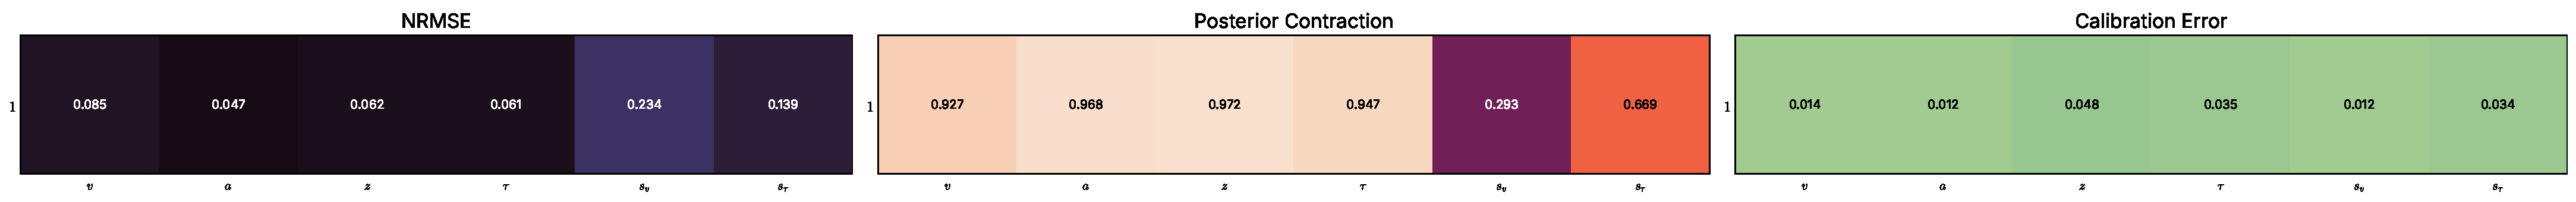
\includegraphics[width=\textwidth]{finetuned/ddm/intercept_only/metrics.pdf}
    \caption{Metrics}
  \end{subfigure}
  \caption{\textbf{After fine-tuning: DDM, \emph{intercept-only} design.} (a) Recovery, (b) calibration, (c) metrics. Every estimated parameter enters as an intercept only (6 coefficients shown). As in Figure~\ref{fig:app3-finetuned-lba-intercept-only}; before fine-tuning: Figure~\ref{fig:app1-ddm-intercept-only-cf}.}
  \label{fig:app3-finetuned-ddm-intercept-only}
\end{figure}

\begin{figure}[p]
  \centering
  \begin{subfigure}{\textwidth}\centering
    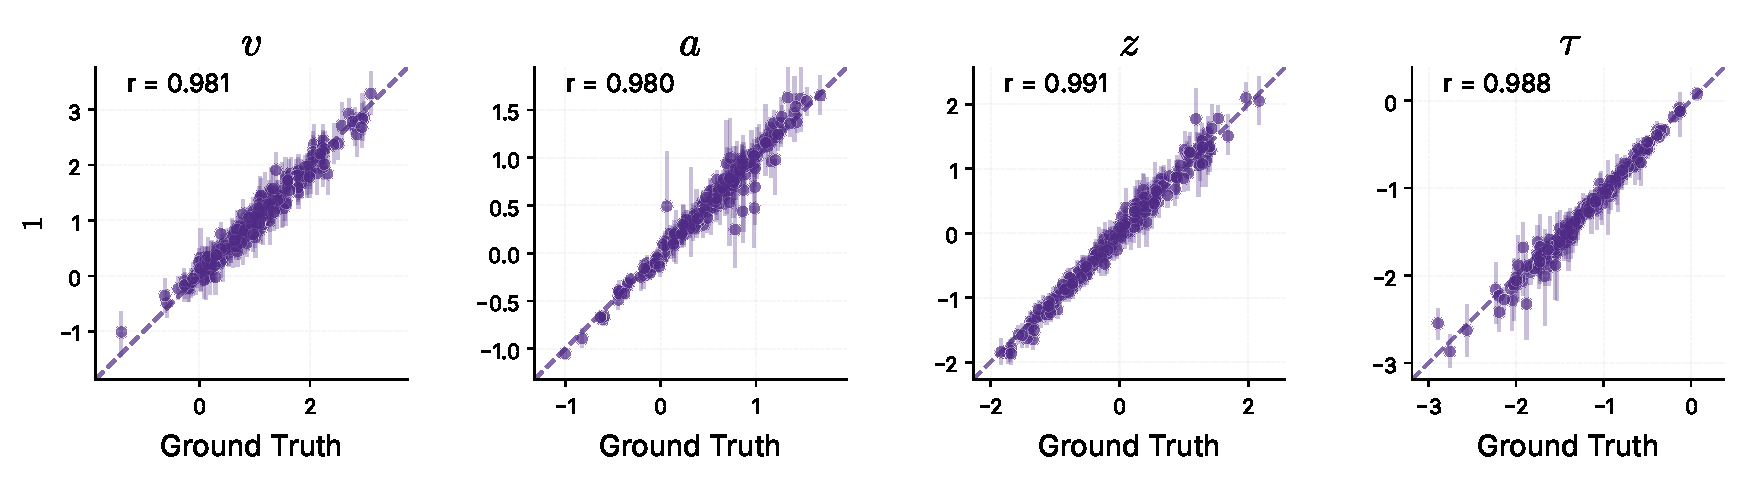
\includegraphics[width=\textwidth,height=0.3\textheight,keepaspectratio]{finetuned/ddm/fixed/recovery.pdf}
    \caption{Recovery}
  \end{subfigure}\\[1ex]
  \begin{subfigure}{\textwidth}\centering
    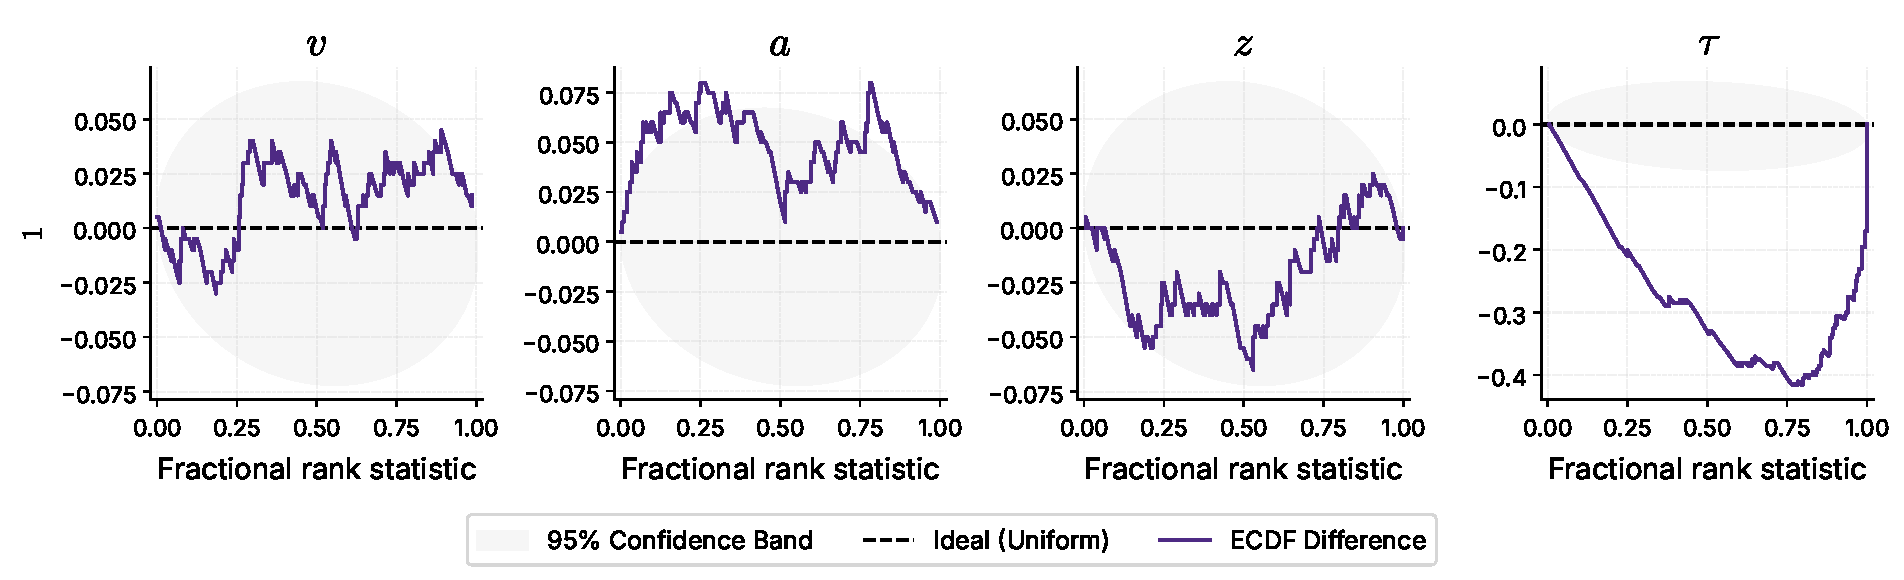
\includegraphics[width=\textwidth,height=0.3\textheight,keepaspectratio]{finetuned/ddm/fixed/ecdf.pdf}
    \caption{Calibration (ECDF)}
  \end{subfigure}\\[1ex]
  \begin{subfigure}{\textwidth}\centering
    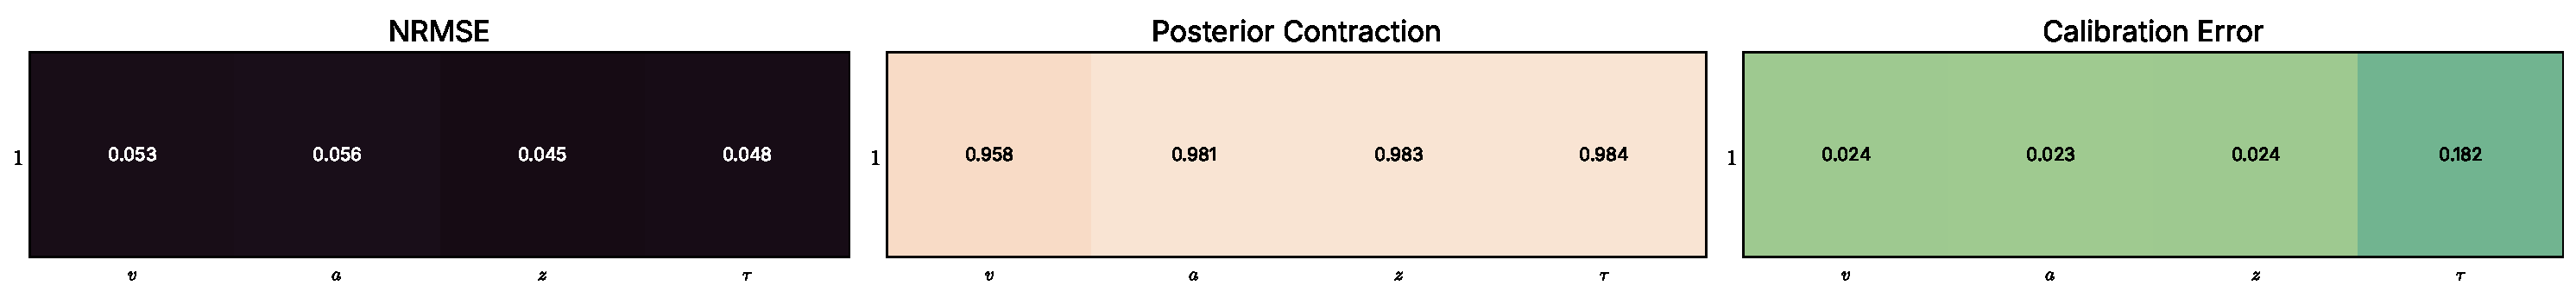
\includegraphics[width=\textwidth]{finetuned/ddm/fixed/metrics.pdf}
    \caption{Metrics}
  \end{subfigure}
  \caption{\textbf{After fine-tuning: DDM, \emph{fixed} design.} (a) Recovery, (b) calibration, (c) metrics. $s_v$ and $s_\tau$ are fixed at 0 and not estimated; every estimated parameter enters as an intercept only (4 coefficients shown). As in Figure~\ref{fig:app3-finetuned-lba-intercept-only}; before fine-tuning: Figure~\ref{fig:app1-ddm-fixed-cf}.}
  \label{fig:app3-finetuned-ddm-fixed}
\end{figure}

\begin{figure}[p]
  \centering
  \begin{subfigure}{\textwidth}\centering
    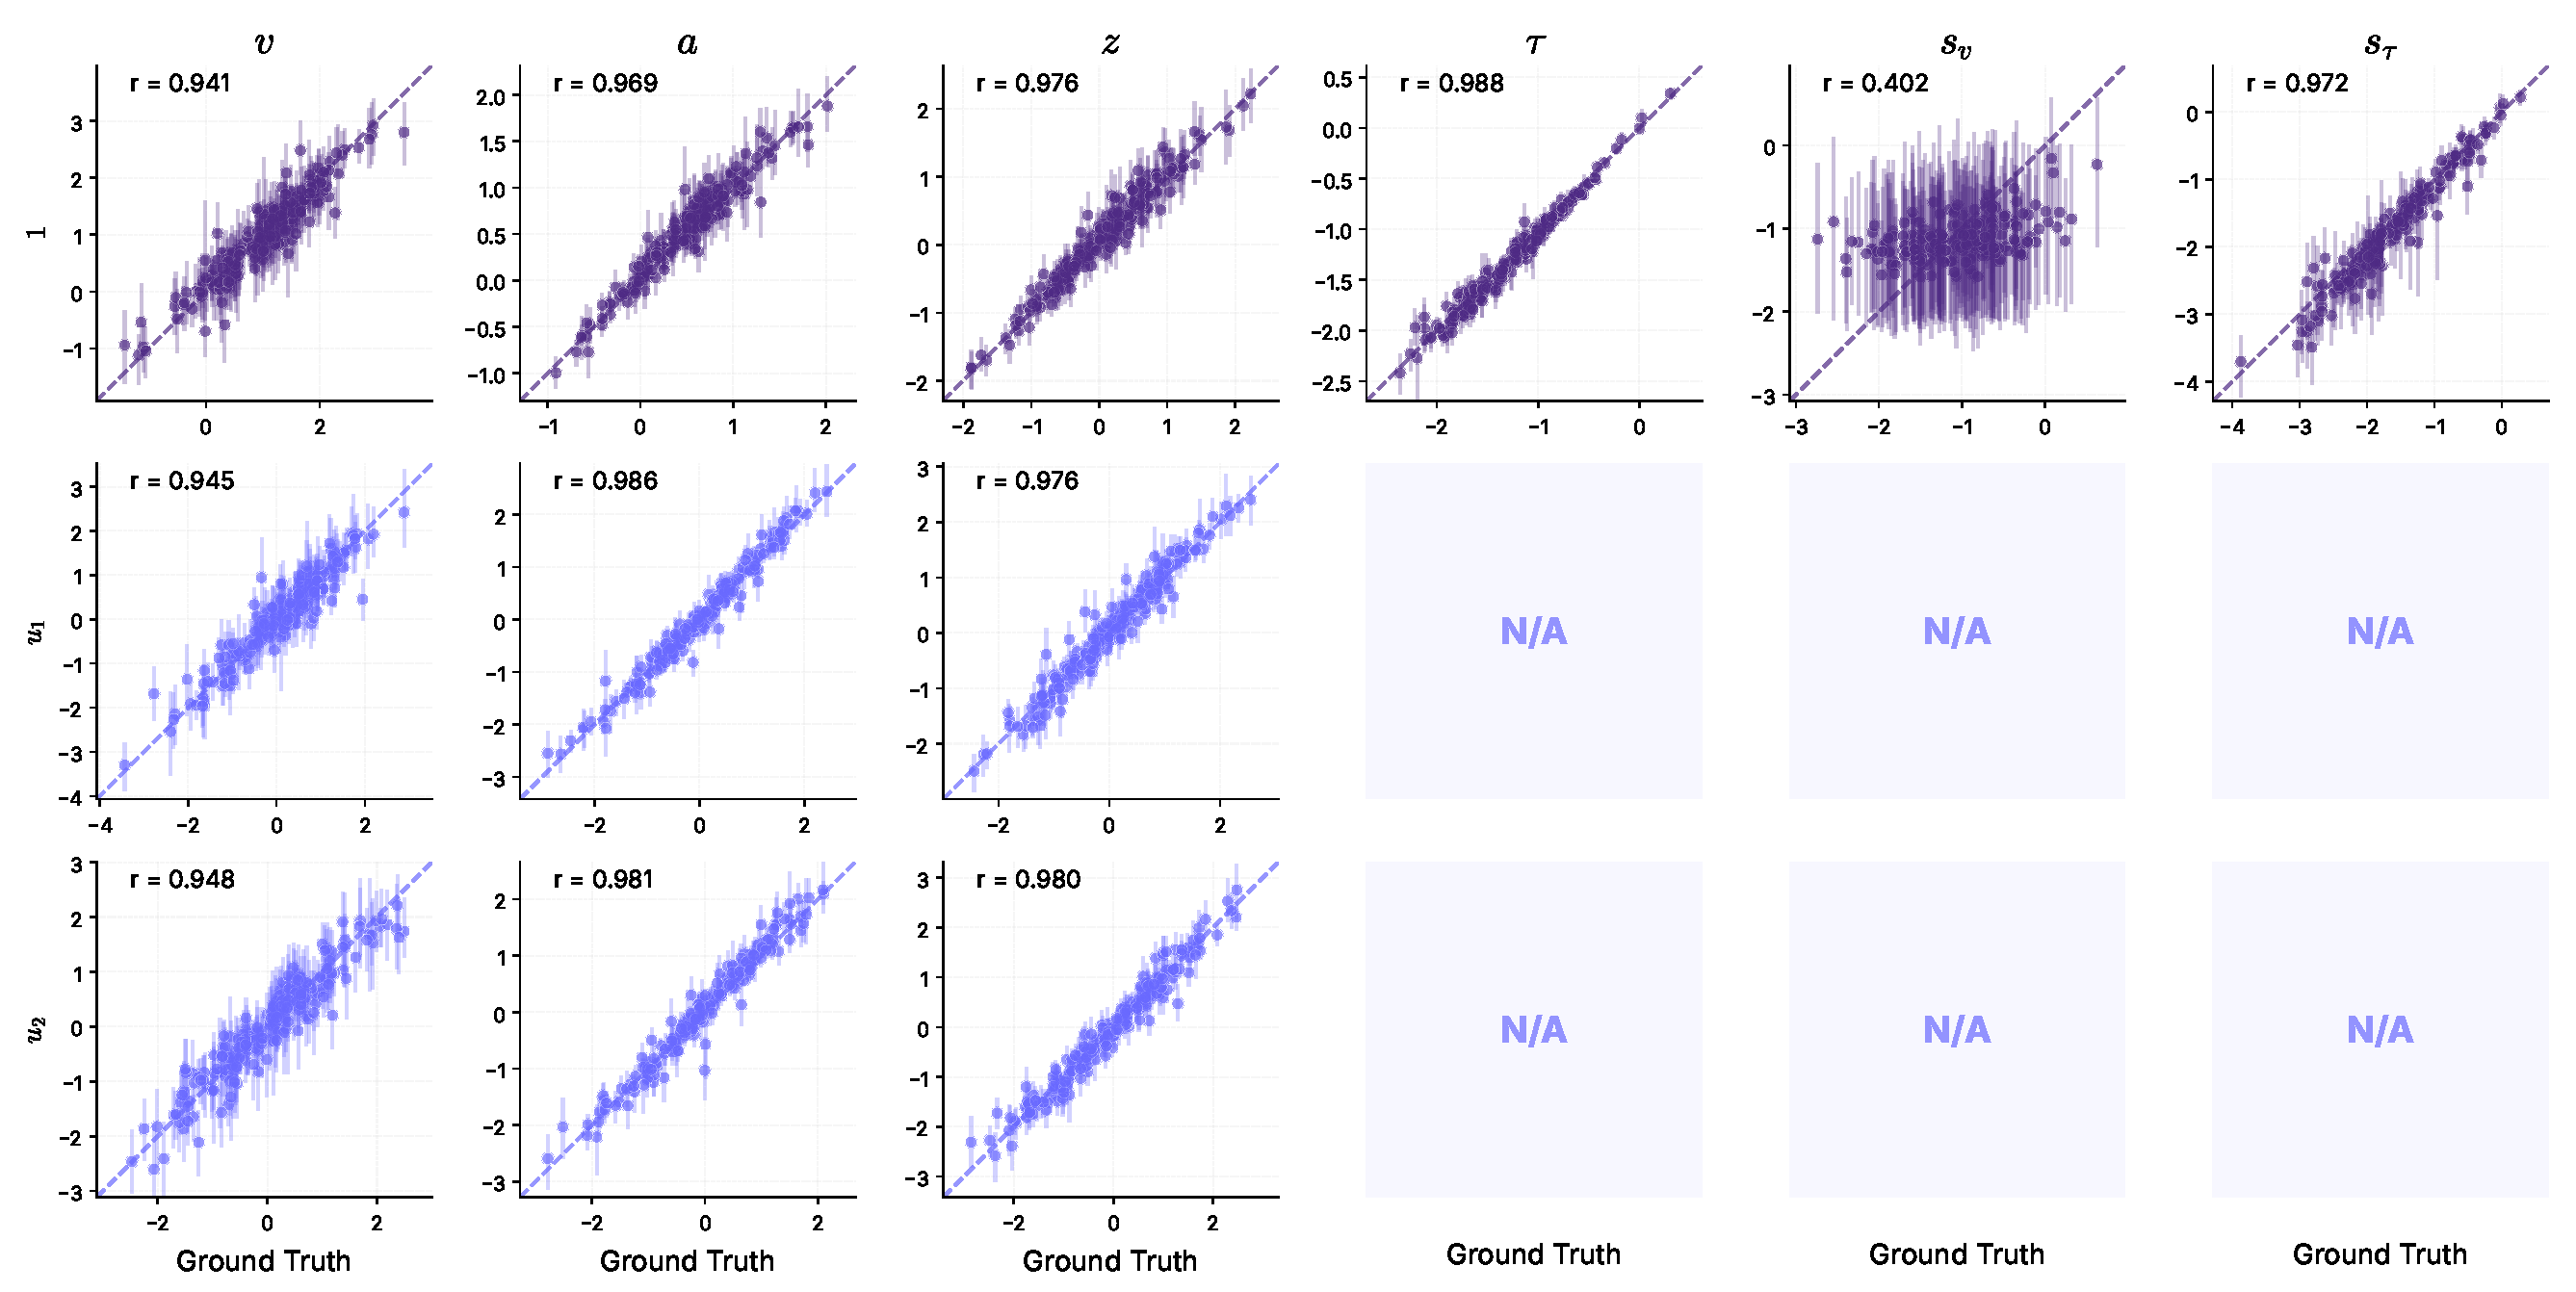
\includegraphics[width=\textwidth,height=0.3\textheight,keepaspectratio]{finetuned/ddm/regressed/recovery.pdf}
    \caption{Recovery}
  \end{subfigure}\\[1ex]
  \begin{subfigure}{\textwidth}\centering
    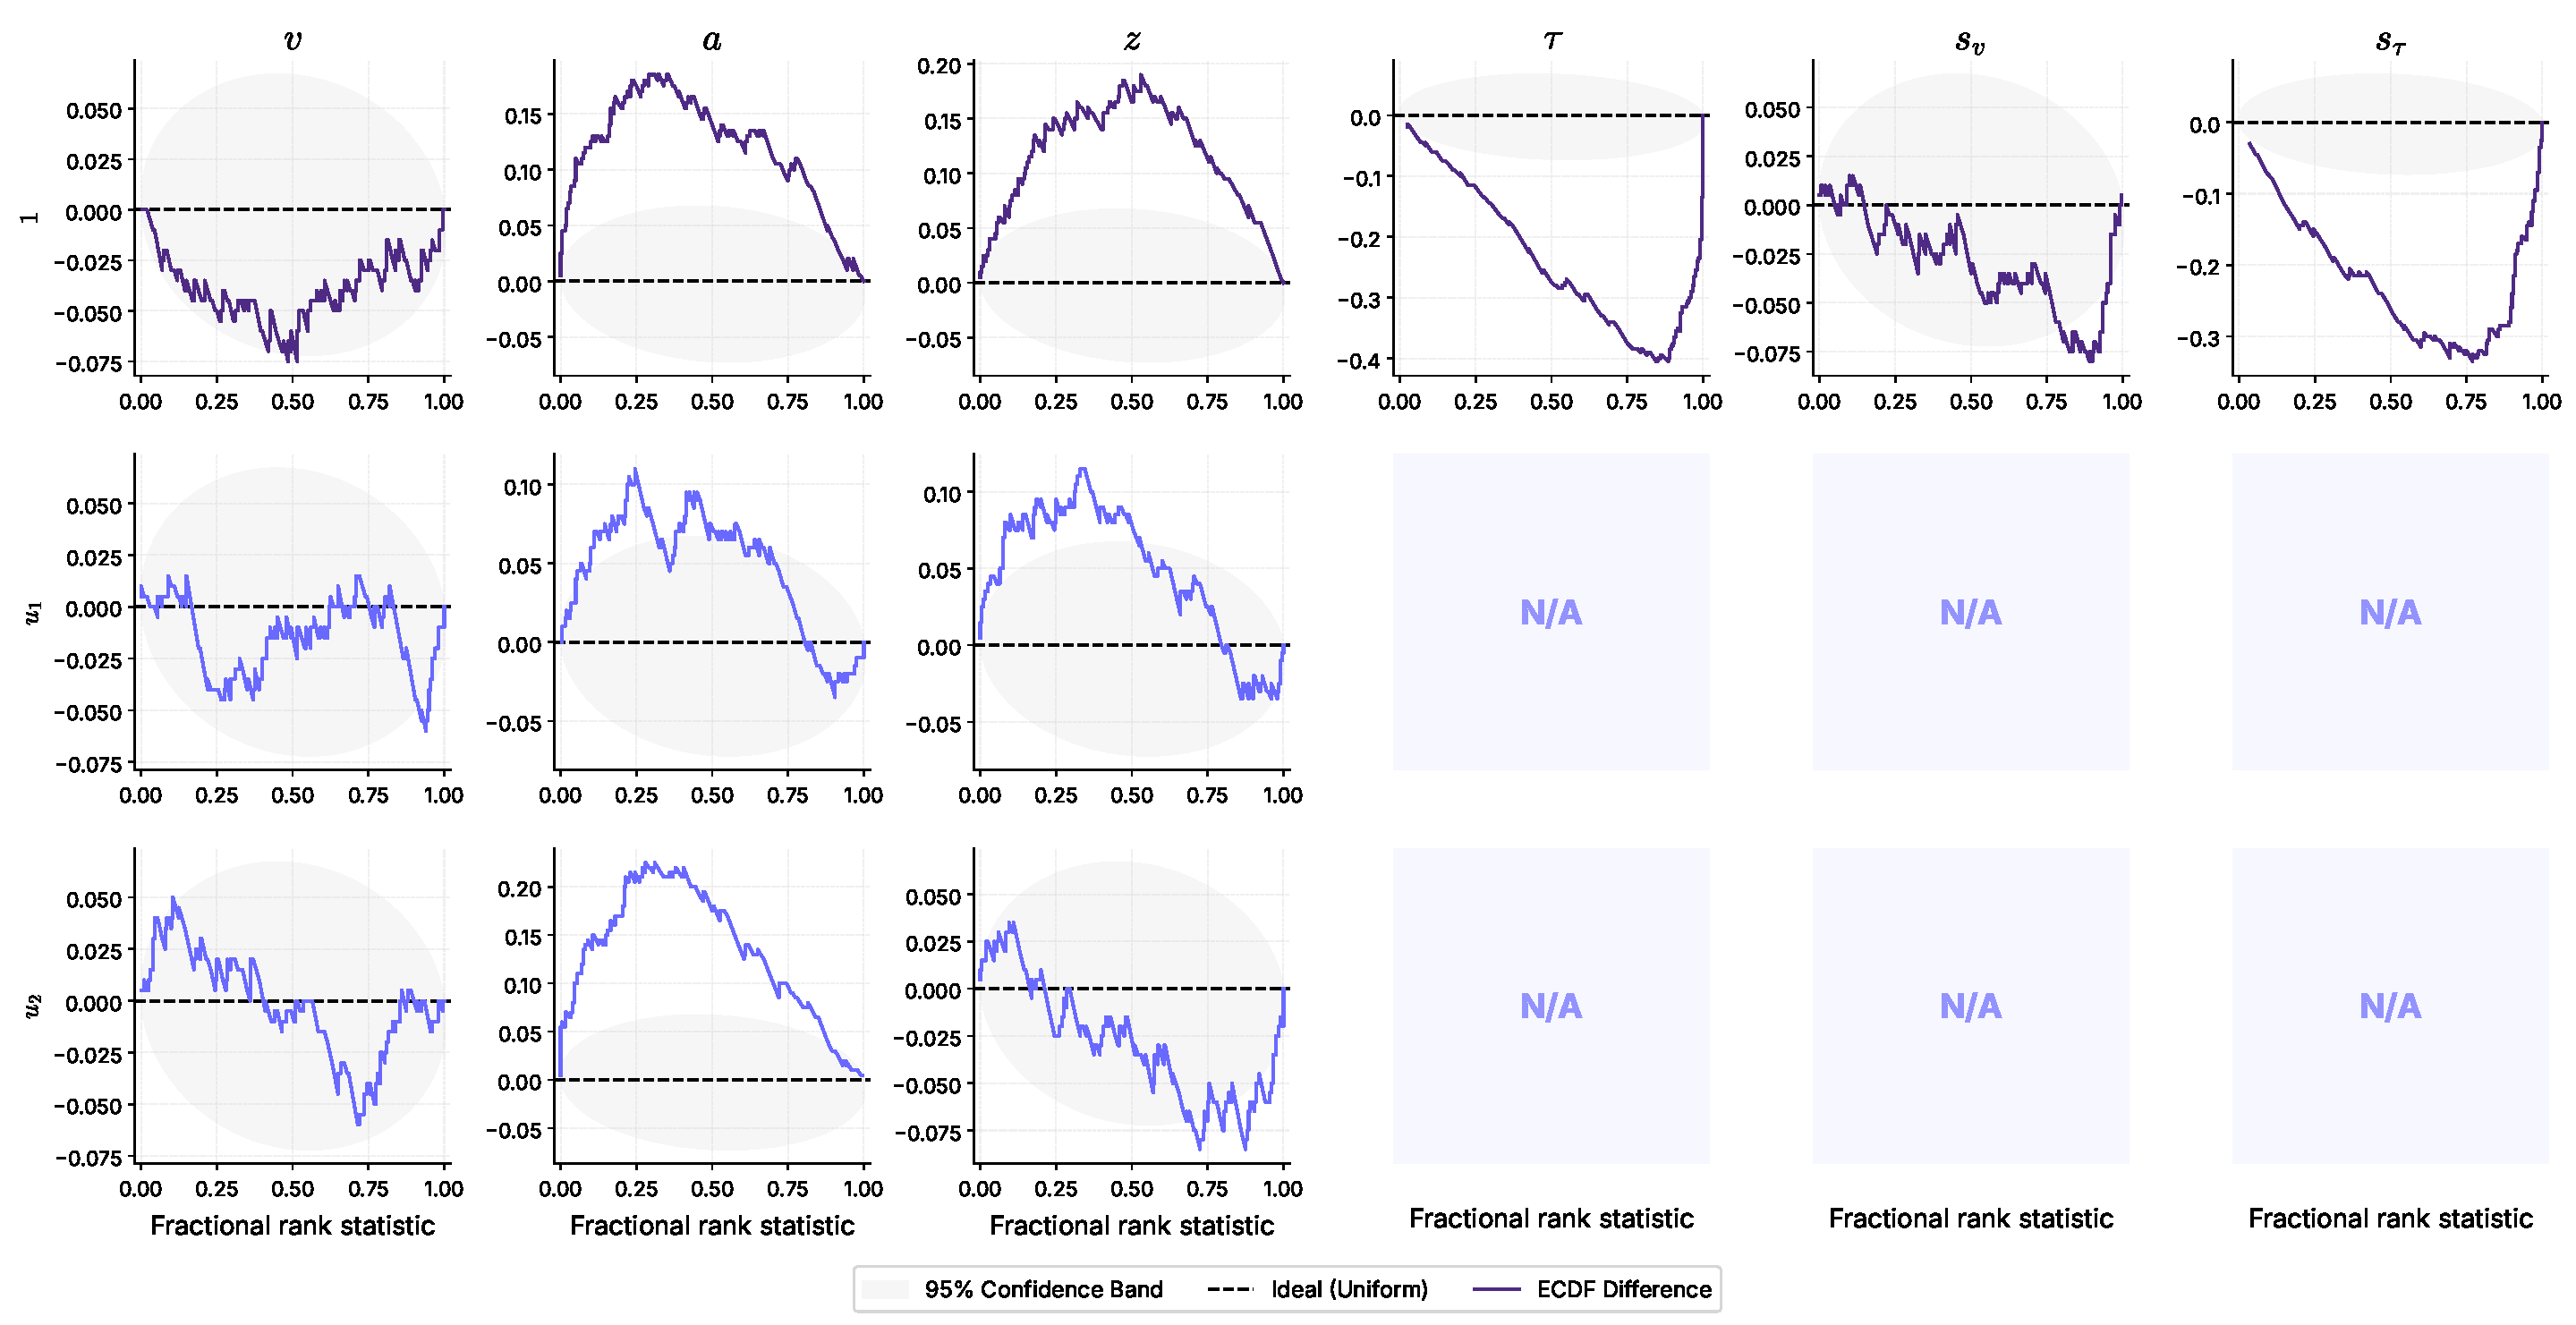
\includegraphics[width=\textwidth,height=0.3\textheight,keepaspectratio]{finetuned/ddm/regressed/ecdf.pdf}
    \caption{Calibration (ECDF)}
  \end{subfigure}\\[1ex]
  \begin{subfigure}{\textwidth}\centering
    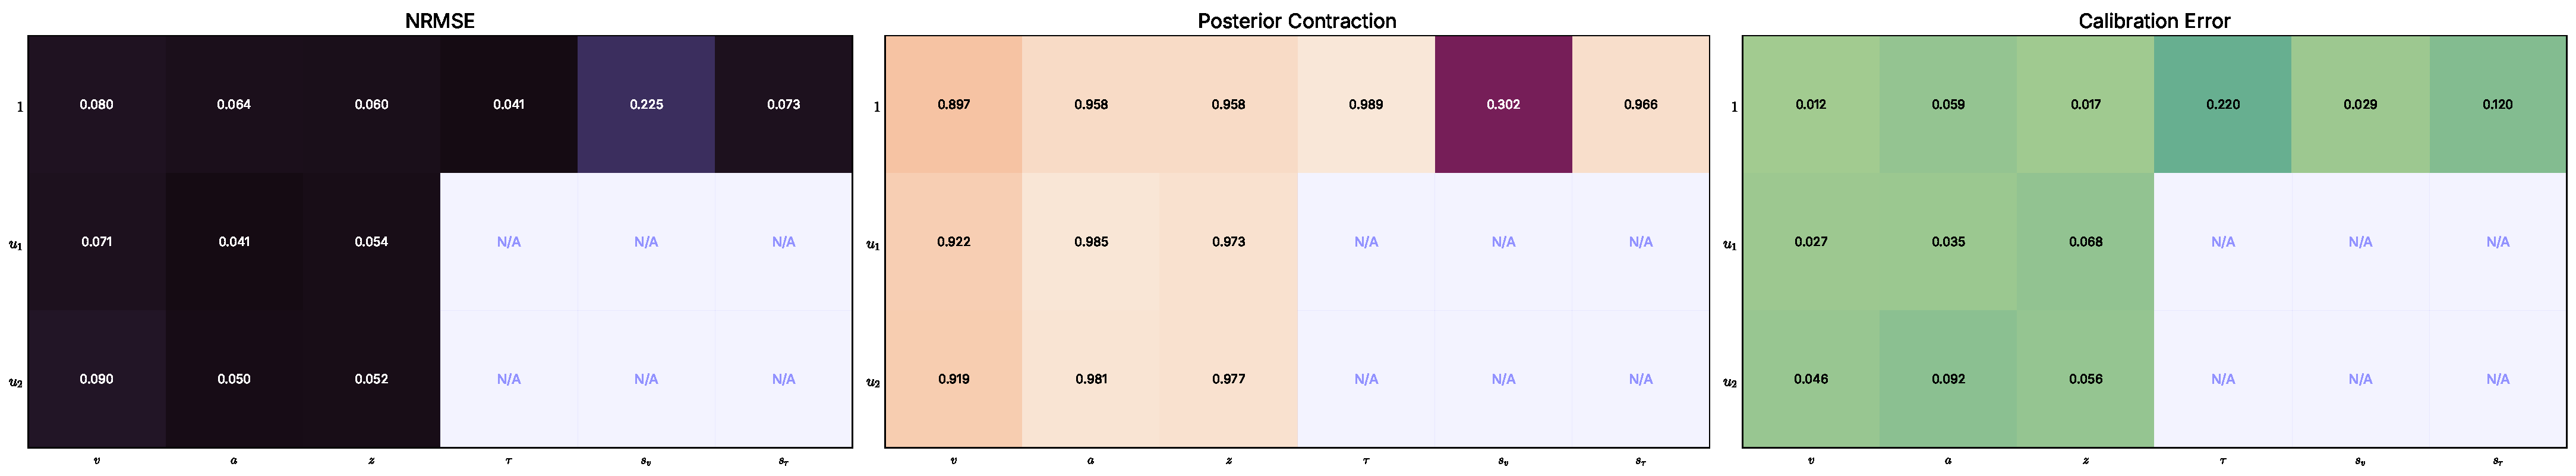
\includegraphics[width=\textwidth]{finetuned/ddm/regressed/metrics.pdf}
    \caption{Metrics}
  \end{subfigure}
  \caption{\textbf{After fine-tuning: DDM, \emph{regressed} design.} (a) Recovery, (b) calibration, (c) metrics. $v$, $a$ and $z$ carry slopes on $u_1$ and $u_2$ (12 coefficients shown). As in Figure~\ref{fig:app3-finetuned-lba-intercept-only}; before fine-tuning: Figure~\ref{fig:app1-ddm-regressed-cf}.}
  \label{fig:app3-finetuned-ddm-regressed}
\end{figure}

\begin{figure}[p]
  \centering
  \begin{subfigure}{\textwidth}\centering
    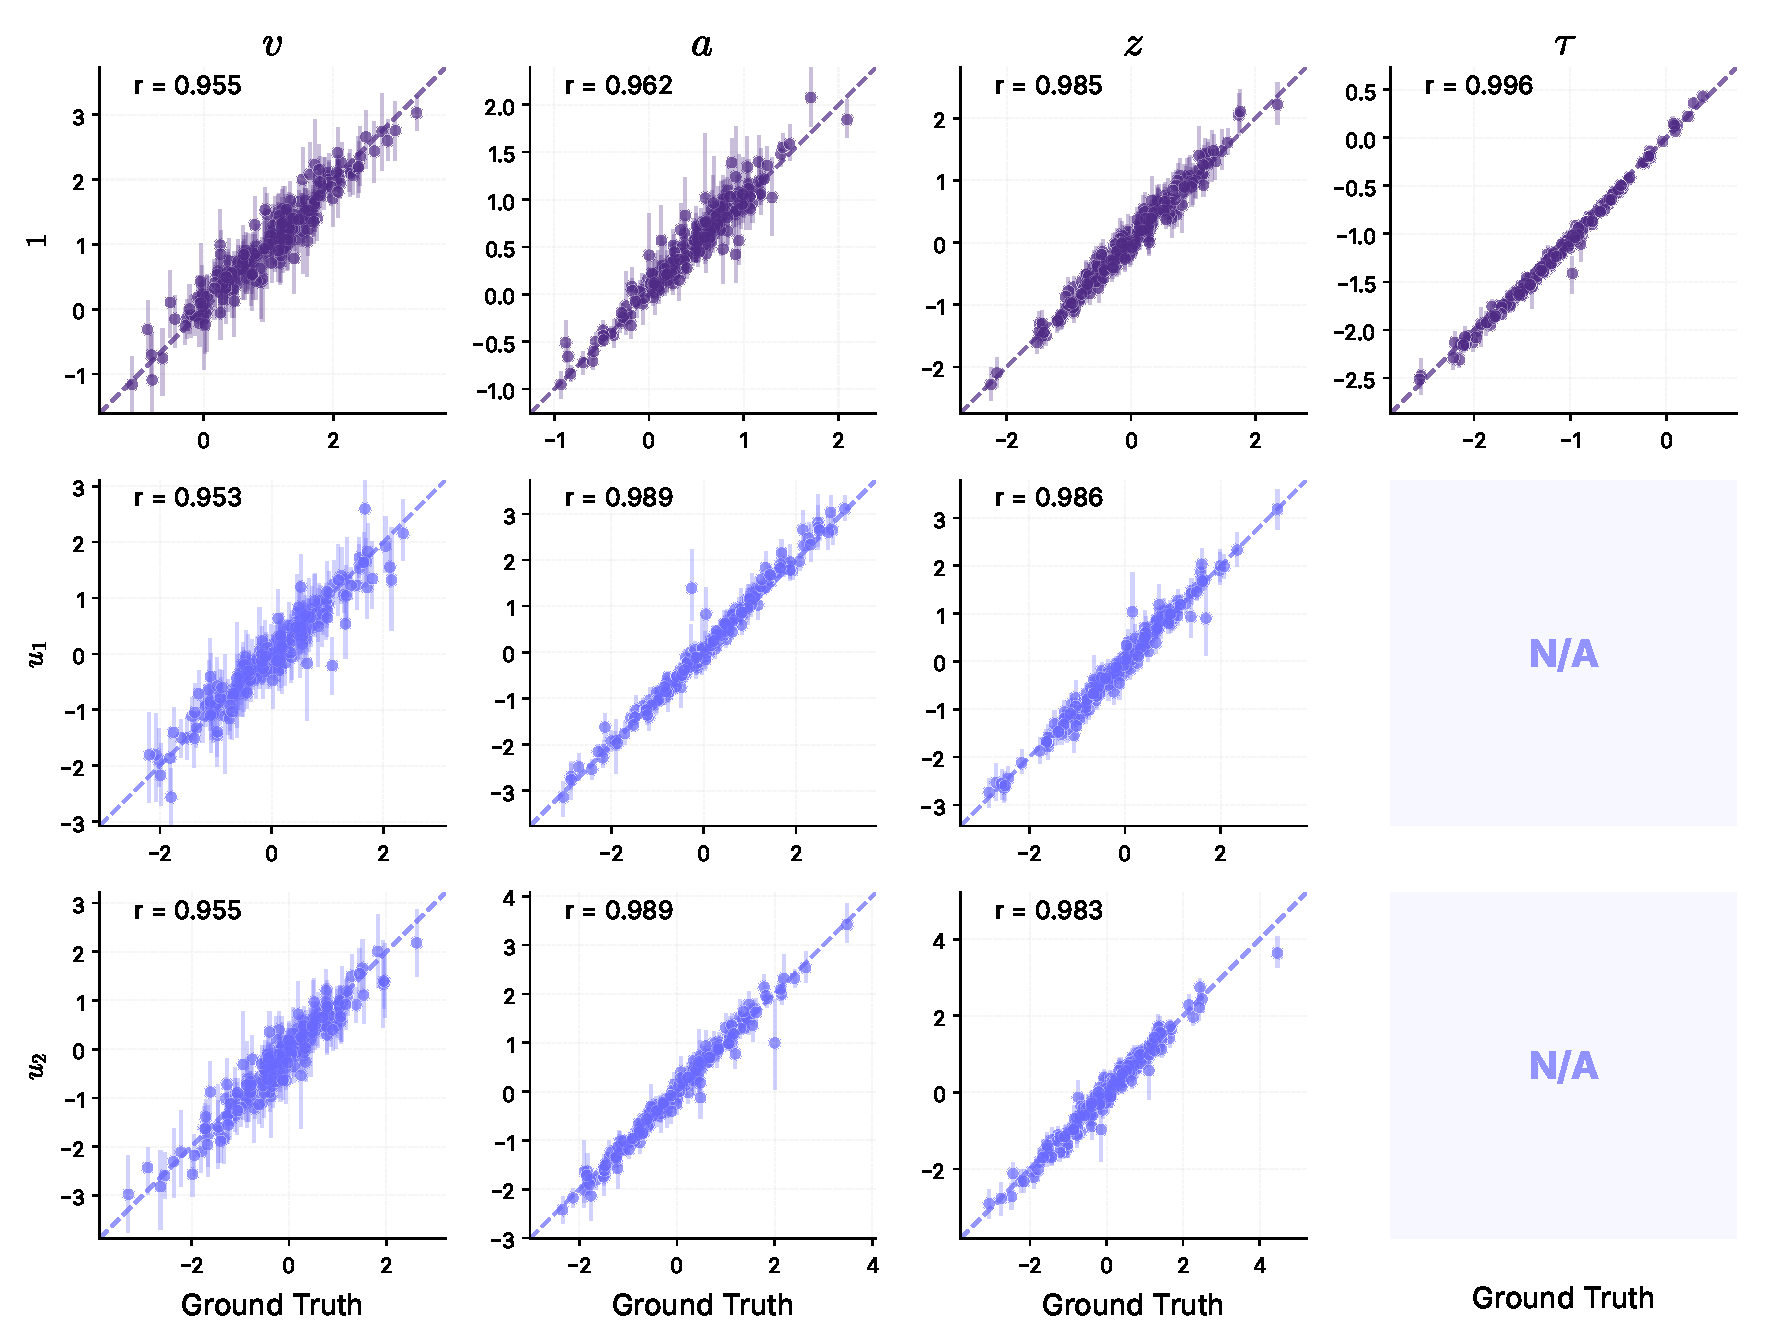
\includegraphics[width=\textwidth,height=0.3\textheight,keepaspectratio]{finetuned/ddm/fixed_regressed/recovery.pdf}
    \caption{Recovery}
  \end{subfigure}\\[1ex]
  \begin{subfigure}{\textwidth}\centering
    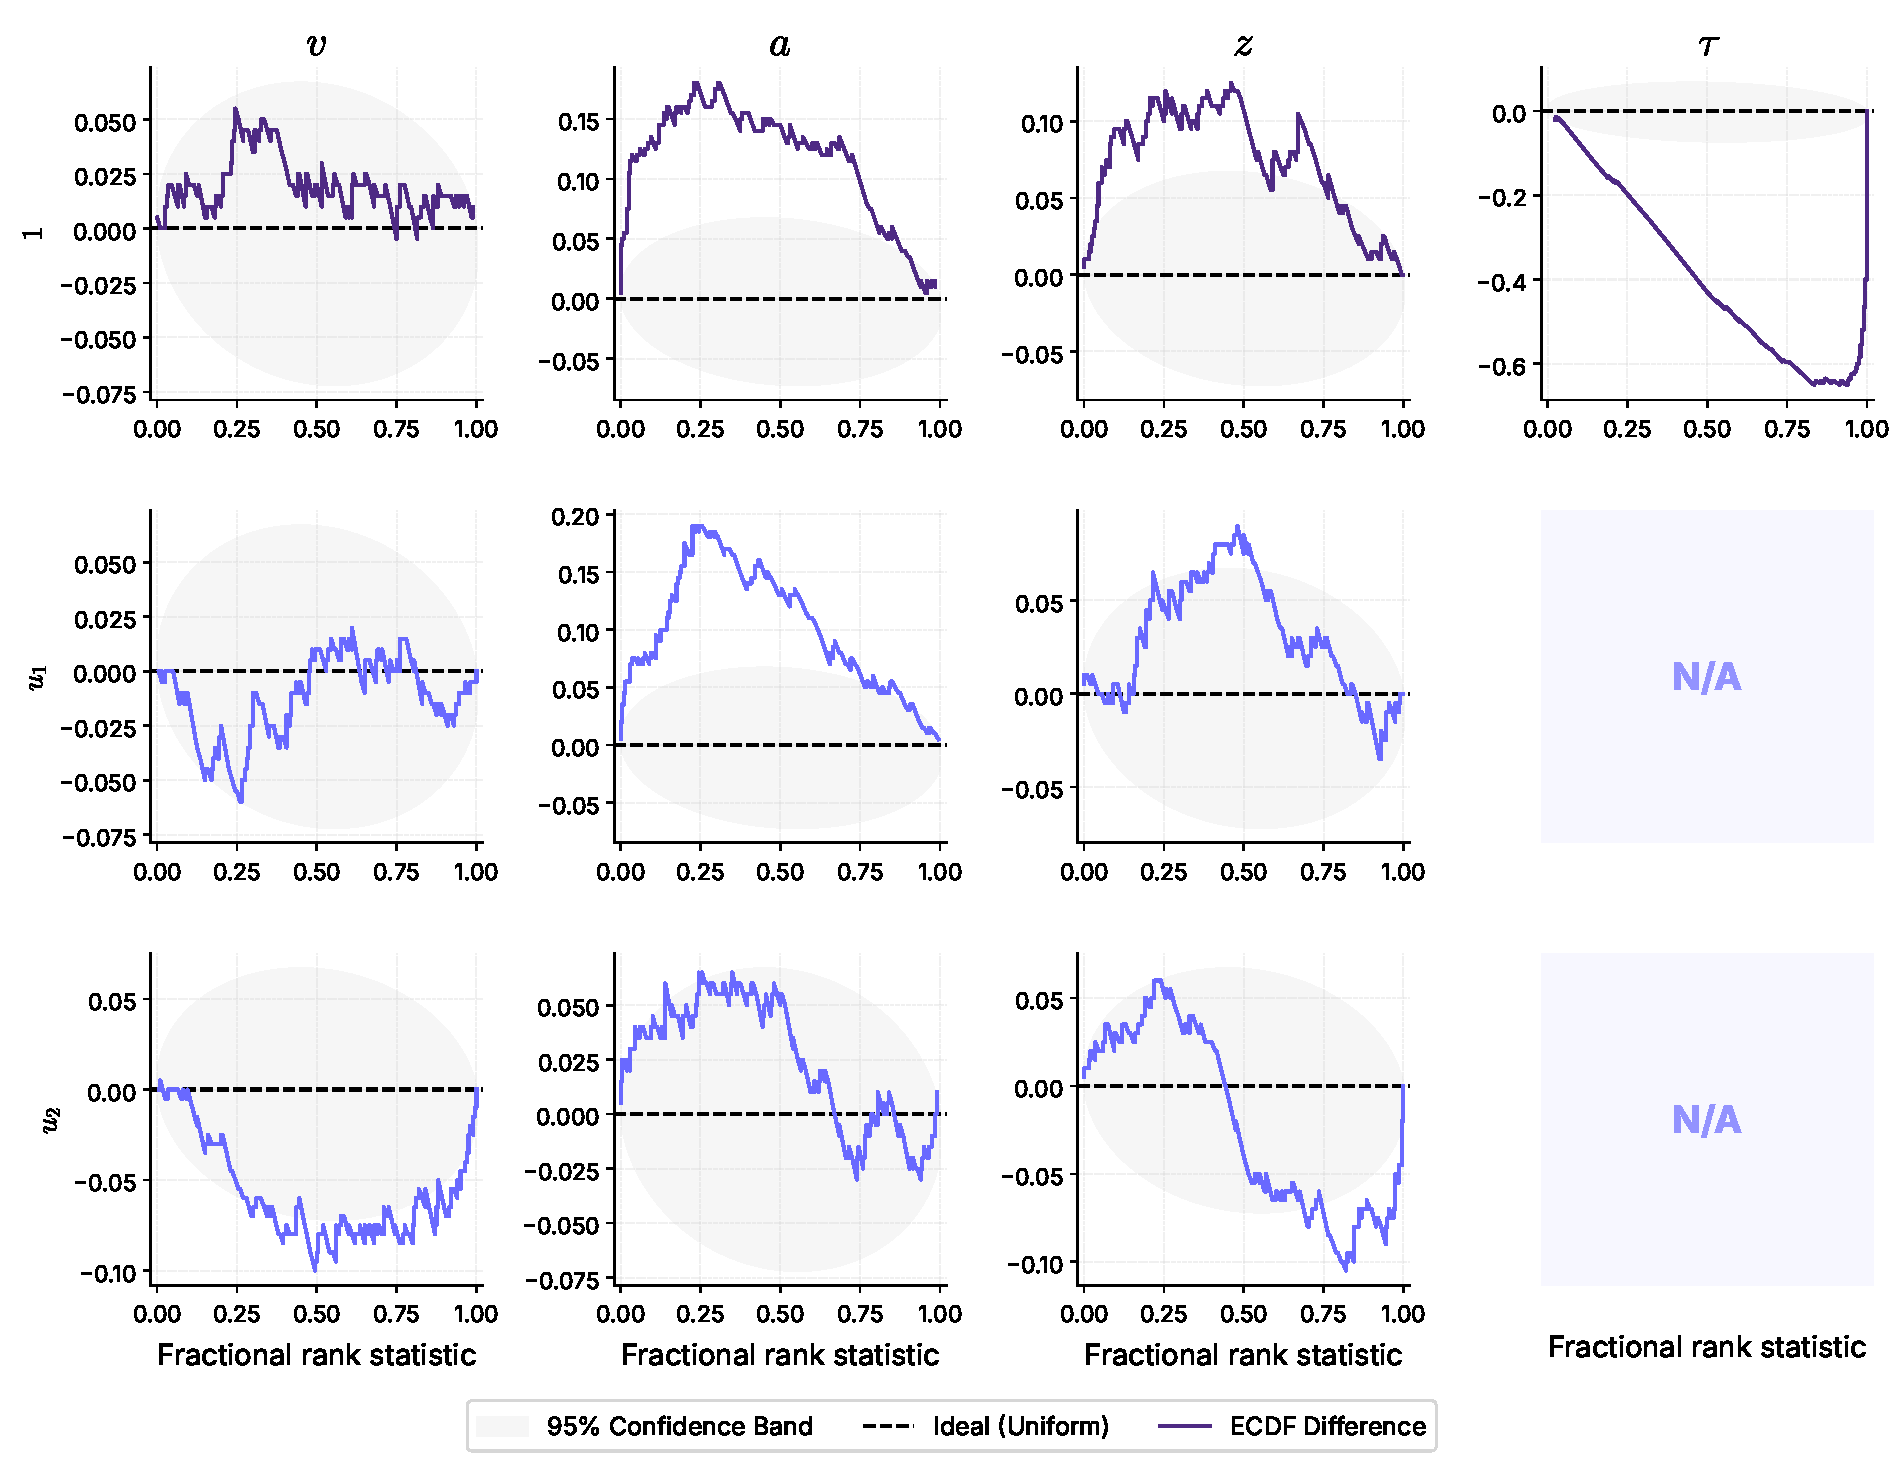
\includegraphics[width=\textwidth,height=0.3\textheight,keepaspectratio]{finetuned/ddm/fixed_regressed/ecdf.pdf}
    \caption{Calibration (ECDF)}
  \end{subfigure}\\[1ex]
  \begin{subfigure}{\textwidth}\centering
    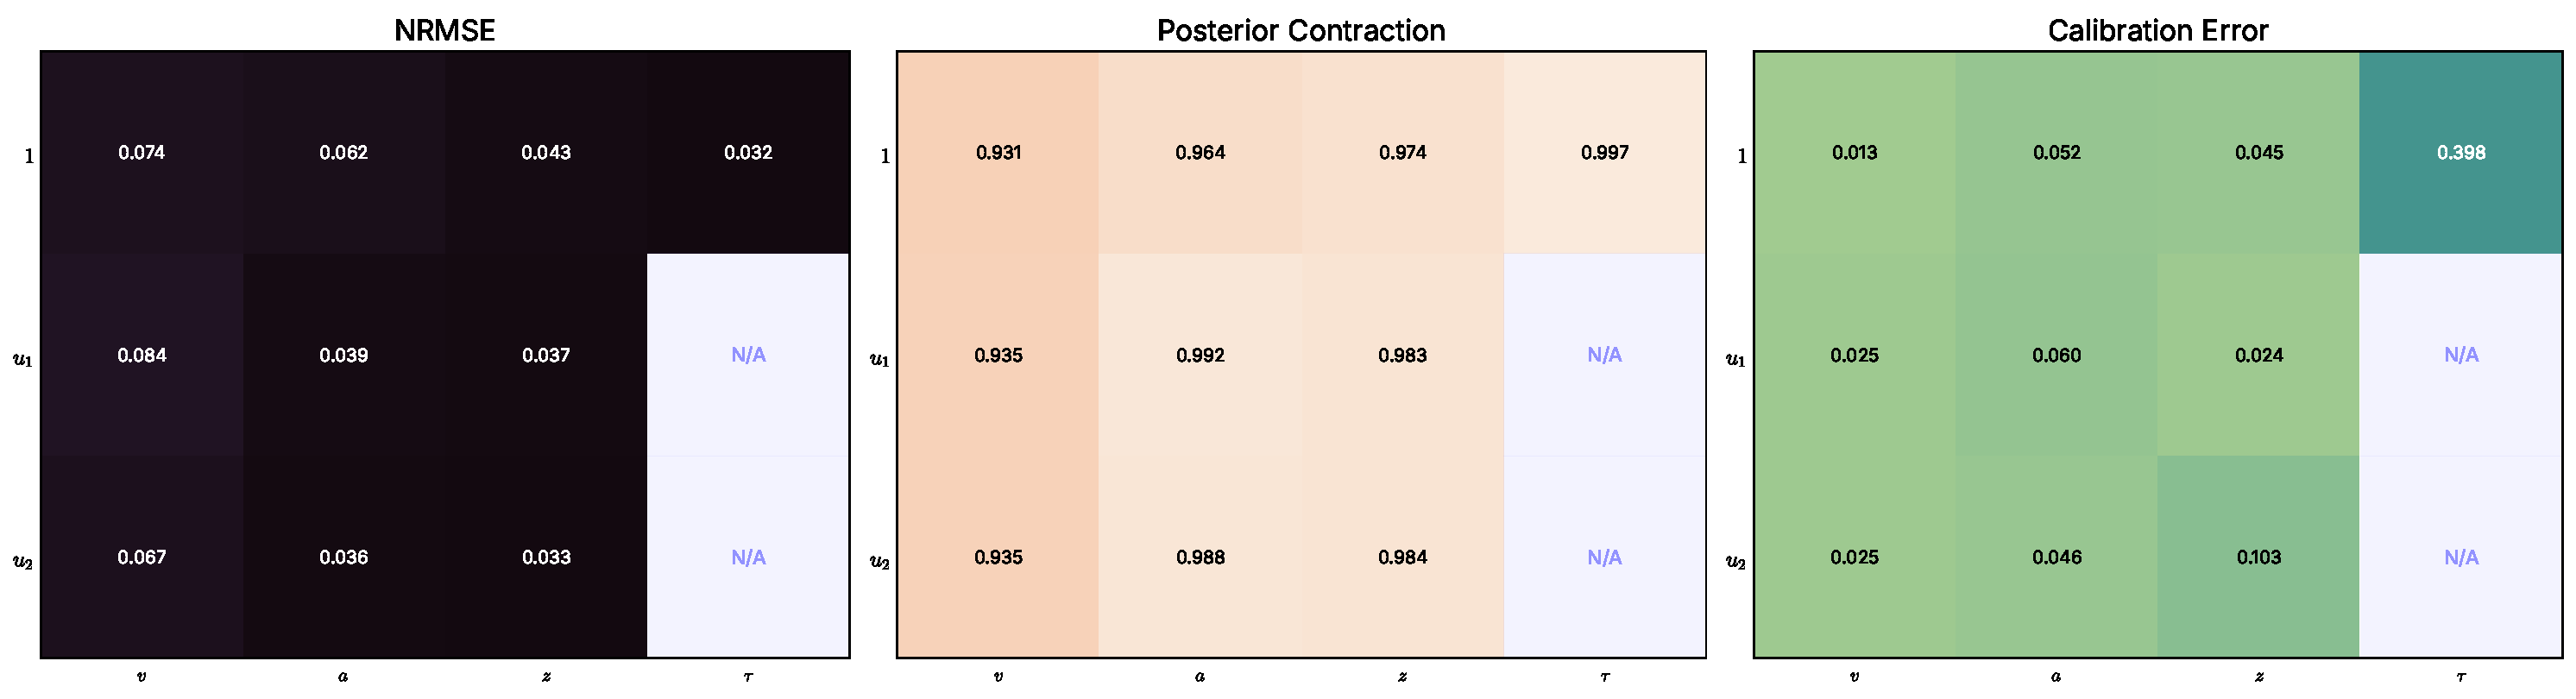
\includegraphics[width=\textwidth]{finetuned/ddm/fixed_regressed/metrics.pdf}
    \caption{Metrics}
  \end{subfigure}
  \caption{\textbf{After fine-tuning: DDM, \emph{fixed + regressed} design.} (a) Recovery, (b) calibration, (c) metrics. $s_v$ and $s_\tau$ are fixed at 0 and not estimated; $v$, $a$ and $z$ carry slopes on $u_1$ and $u_2$ (10 coefficients shown). As in Figure~\ref{fig:app3-finetuned-lba-intercept-only}; before fine-tuning: Figure~\ref{fig:app1-ddm-fixed-regressed-cf}.}
  \label{fig:app3-finetuned-ddm-fixed-regressed}
\end{figure}

\begin{figure}[p]
  \centering
  \begin{subfigure}{\textwidth}\centering
    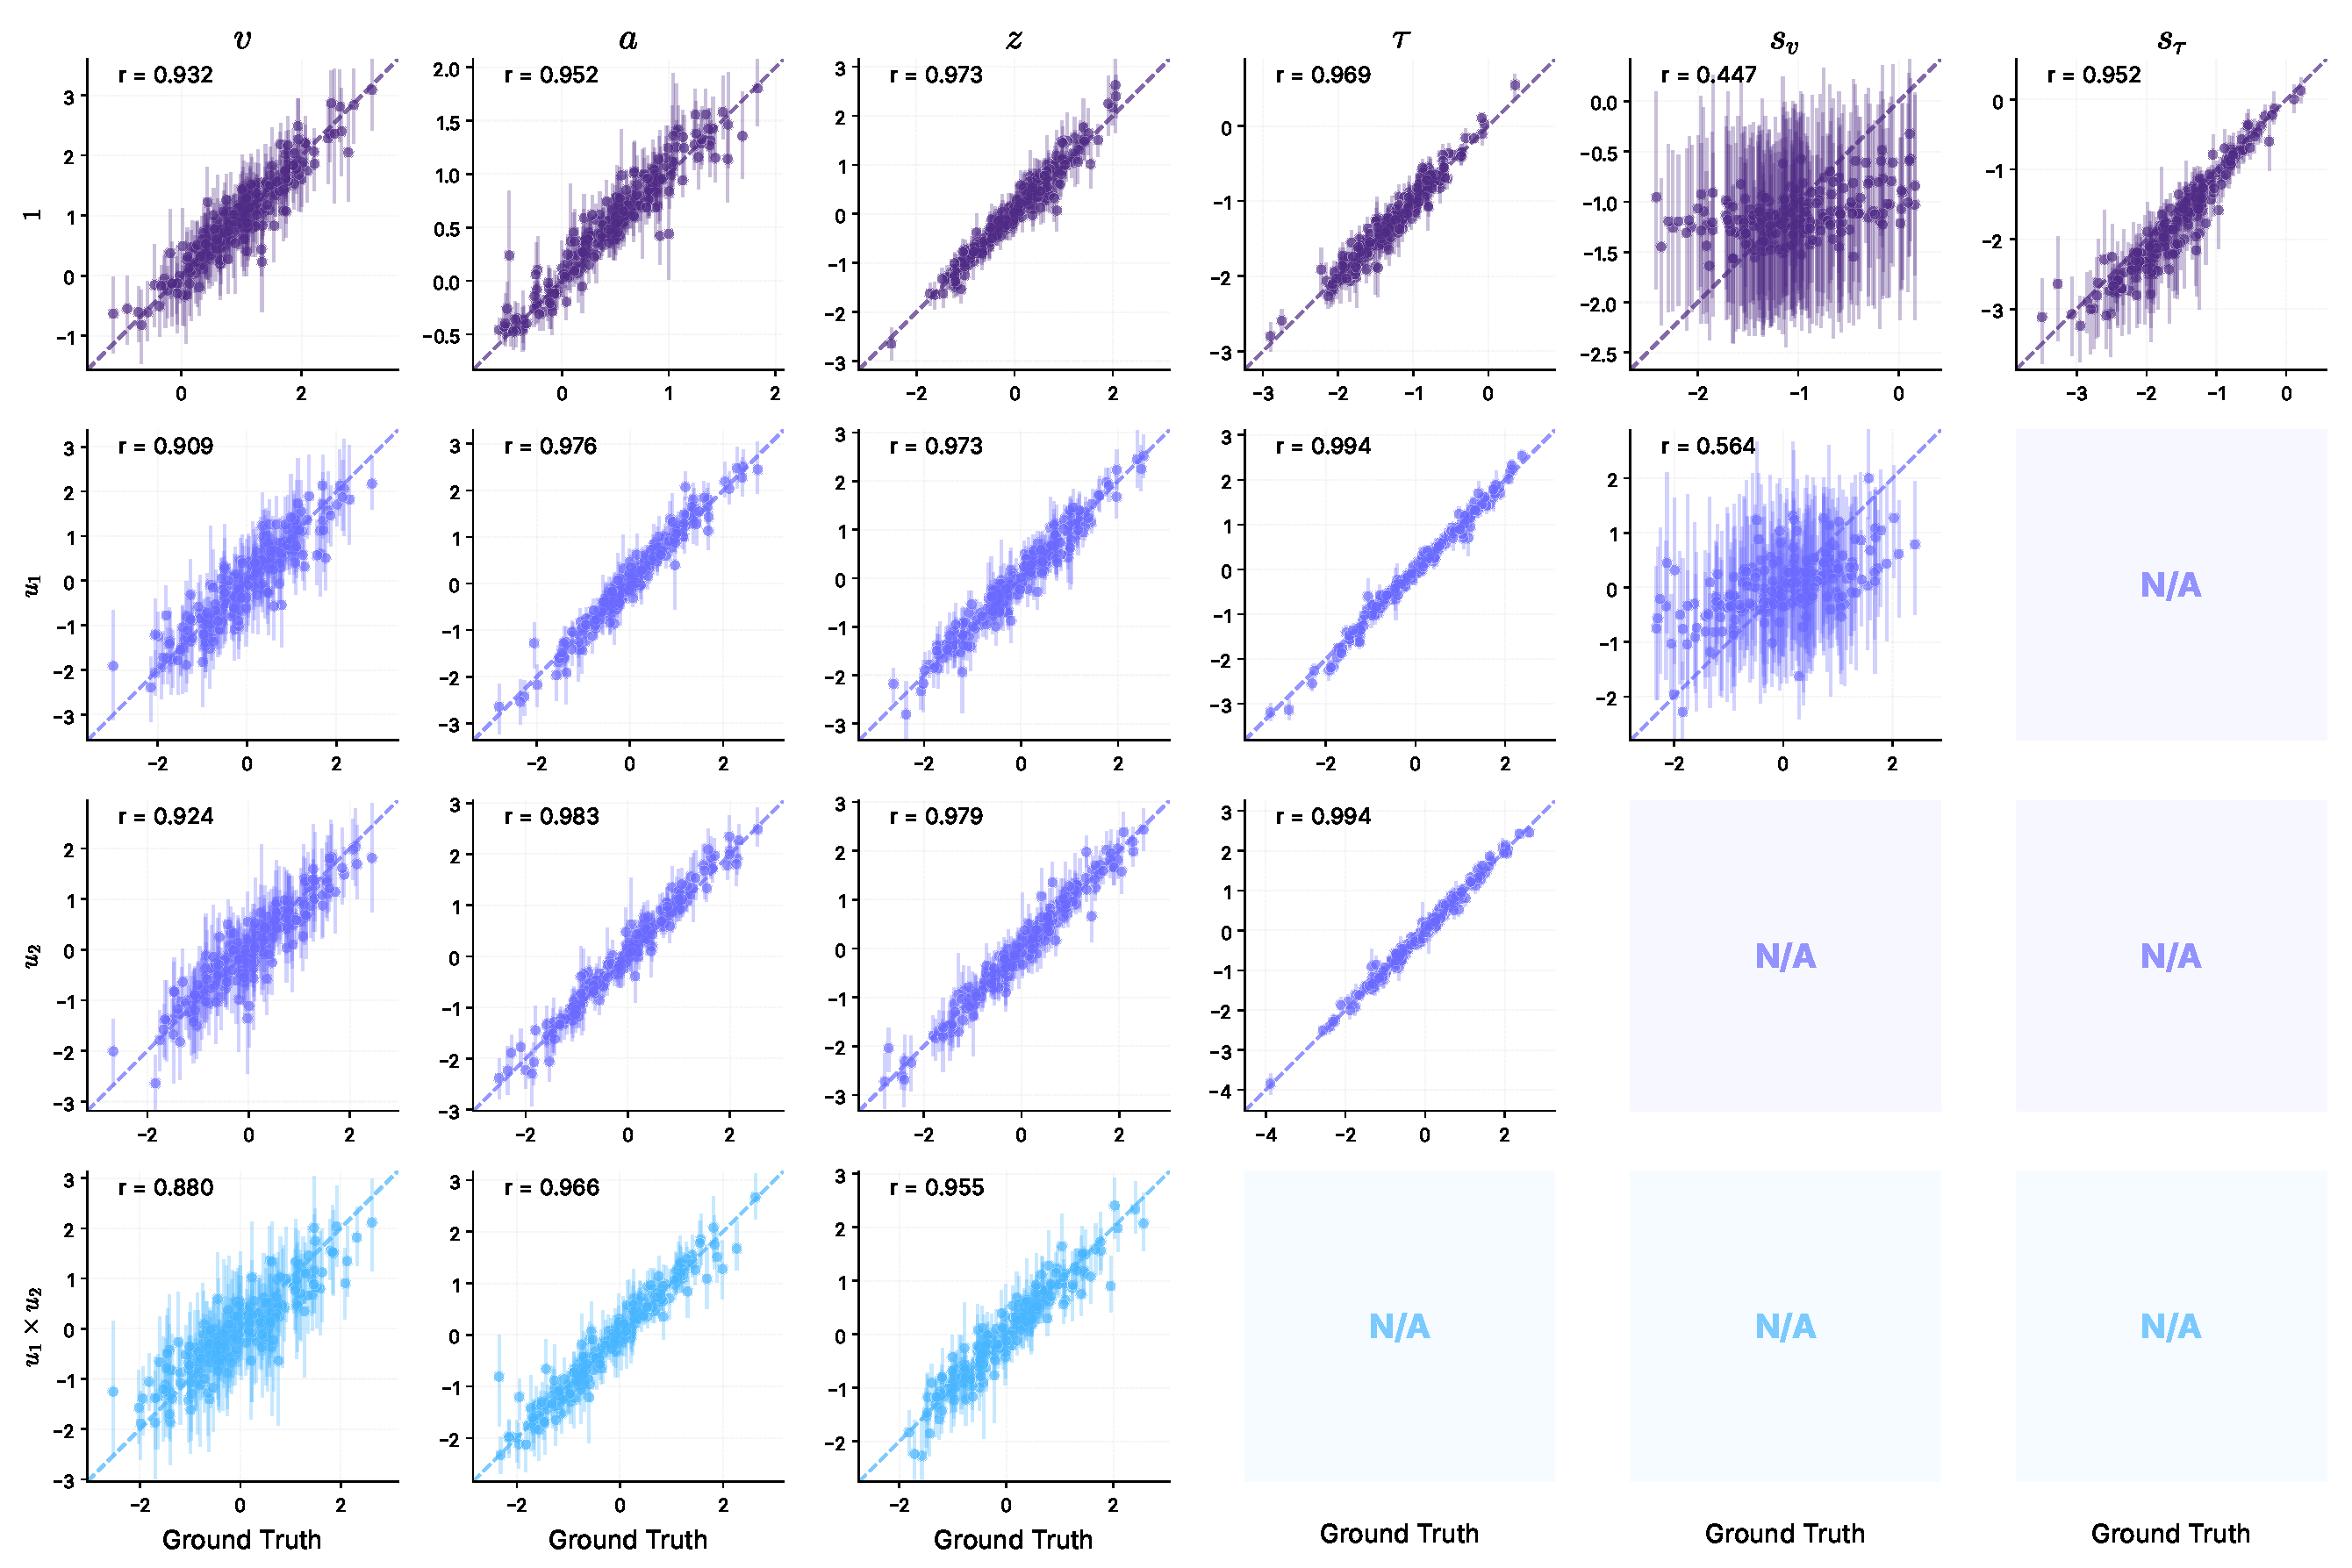
\includegraphics[width=\textwidth,height=0.3\textheight,keepaspectratio]{finetuned/ddm/interaction/recovery.pdf}
    \caption{Recovery}
  \end{subfigure}\\[1ex]
  \begin{subfigure}{\textwidth}\centering
    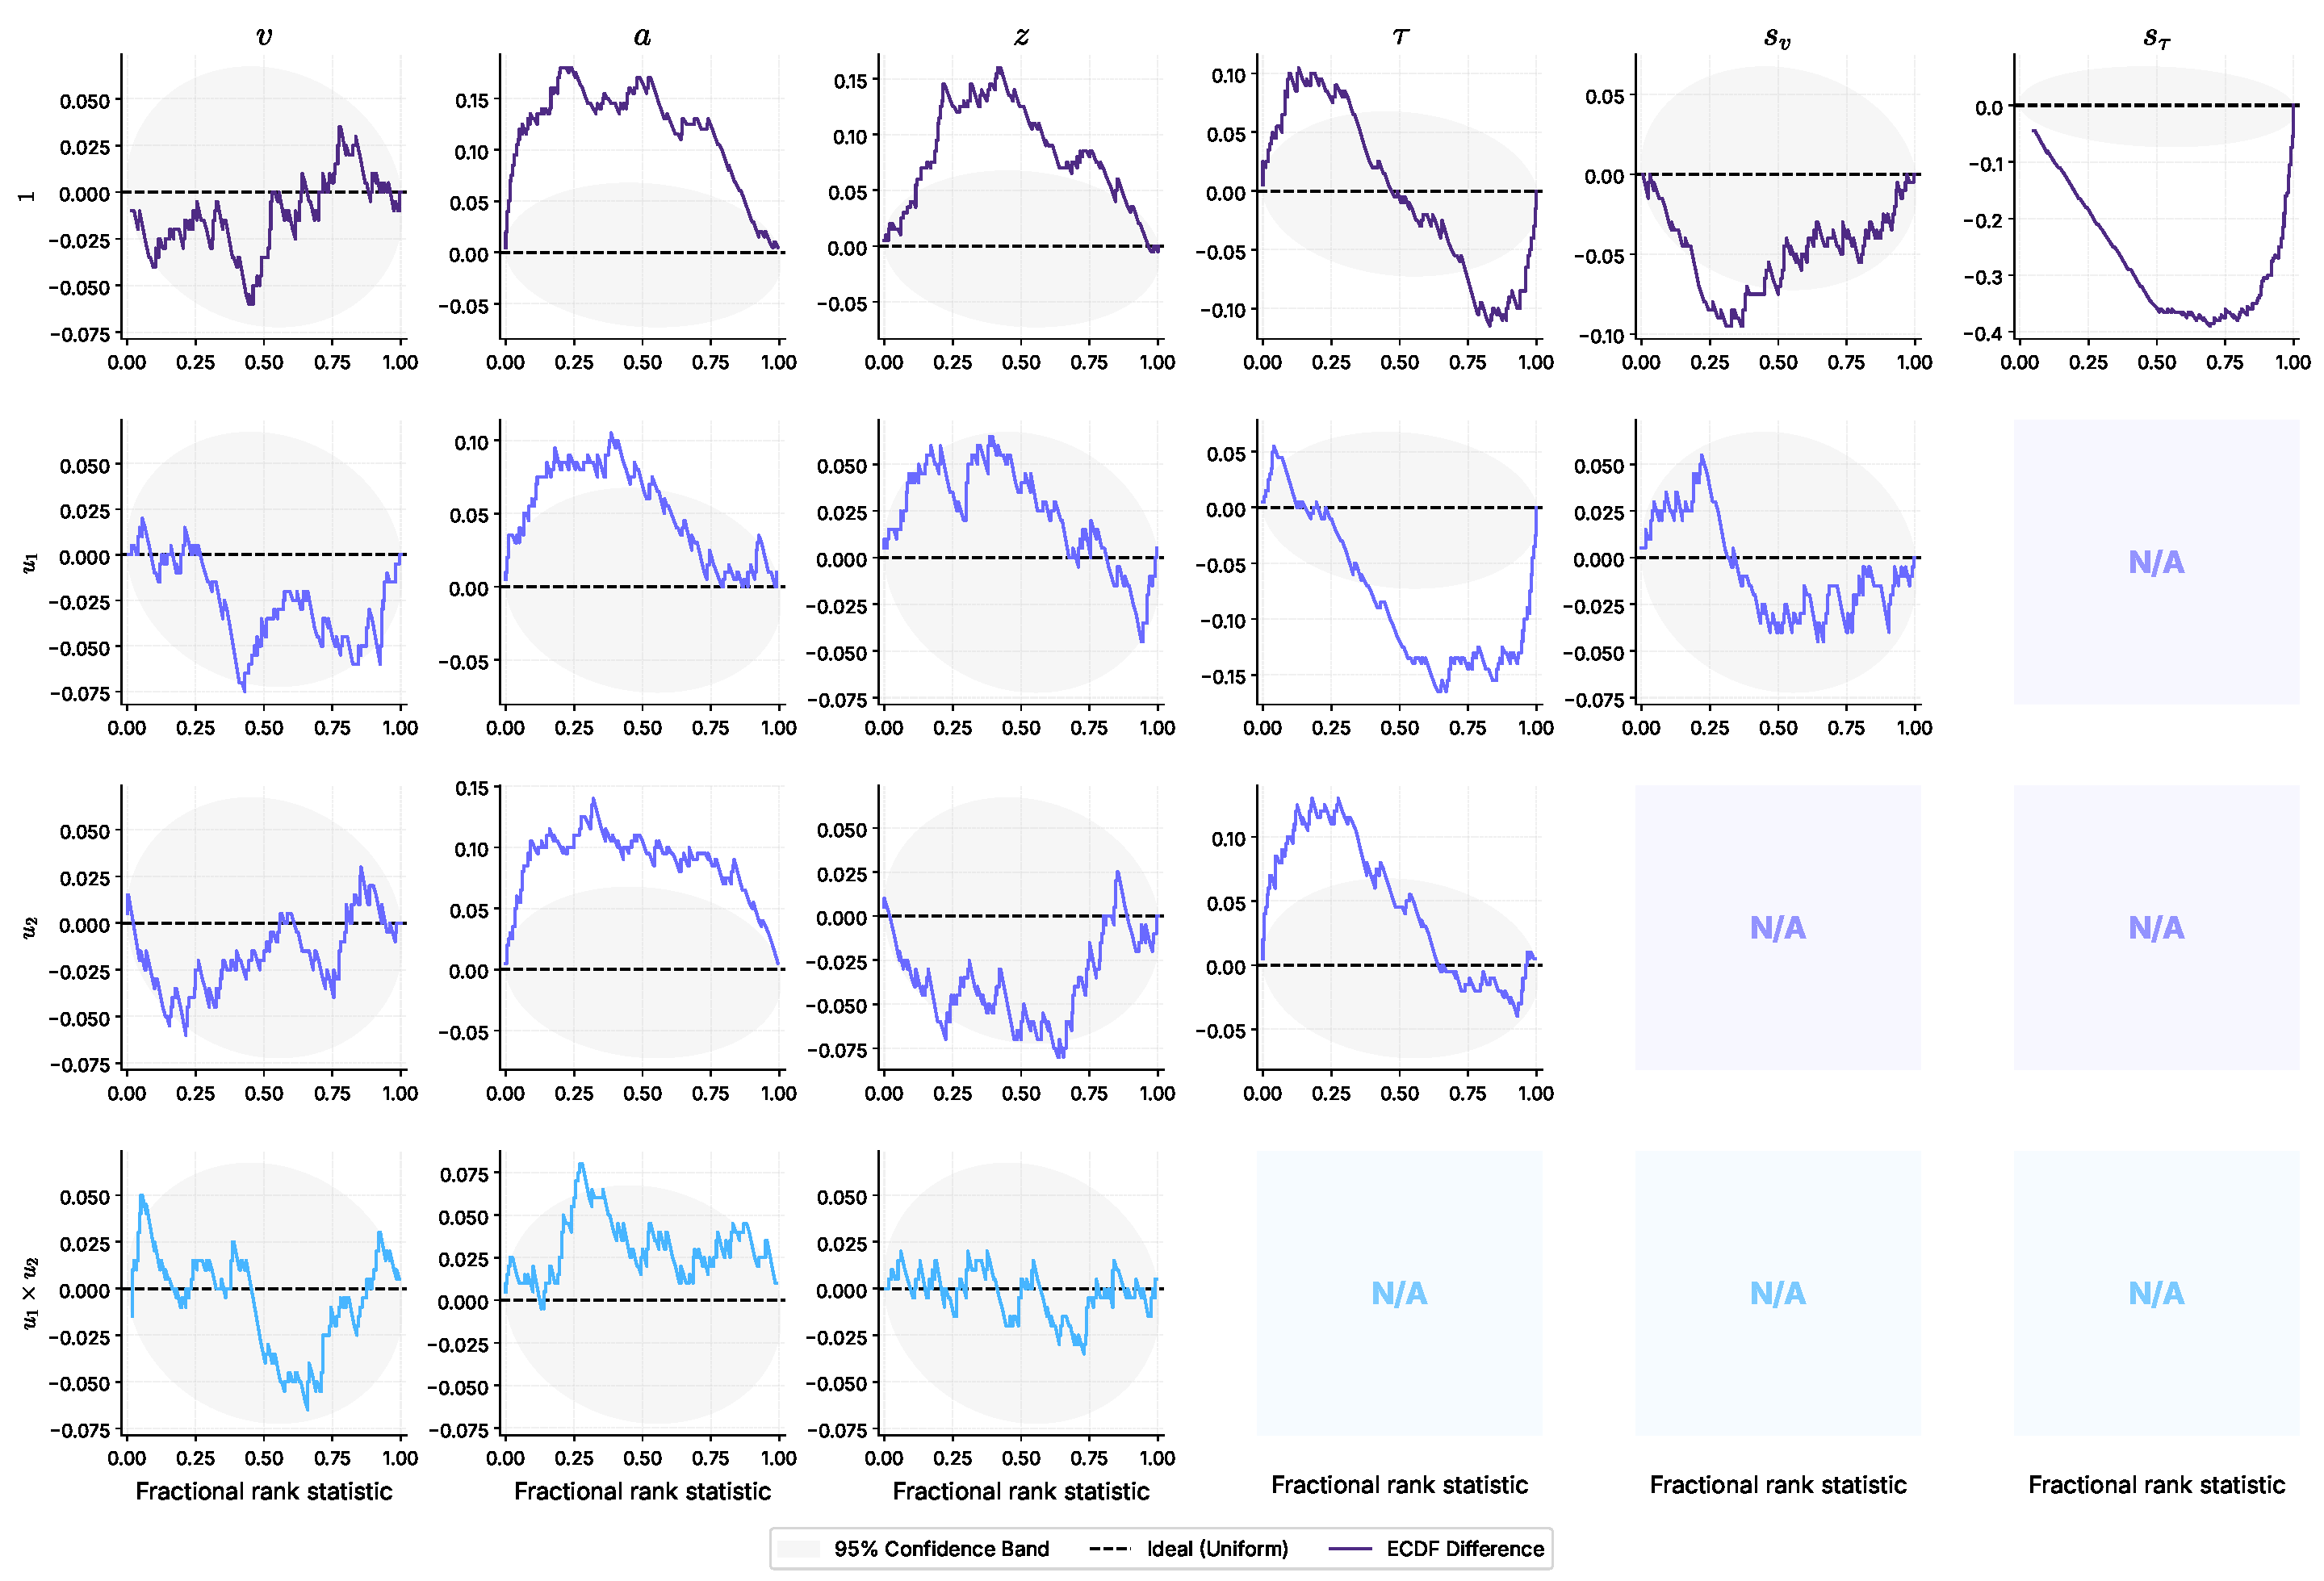
\includegraphics[width=\textwidth,height=0.3\textheight,keepaspectratio]{finetuned/ddm/interaction/ecdf.pdf}
    \caption{Calibration (ECDF)}
  \end{subfigure}\\[1ex]
  \begin{subfigure}{\textwidth}\centering
    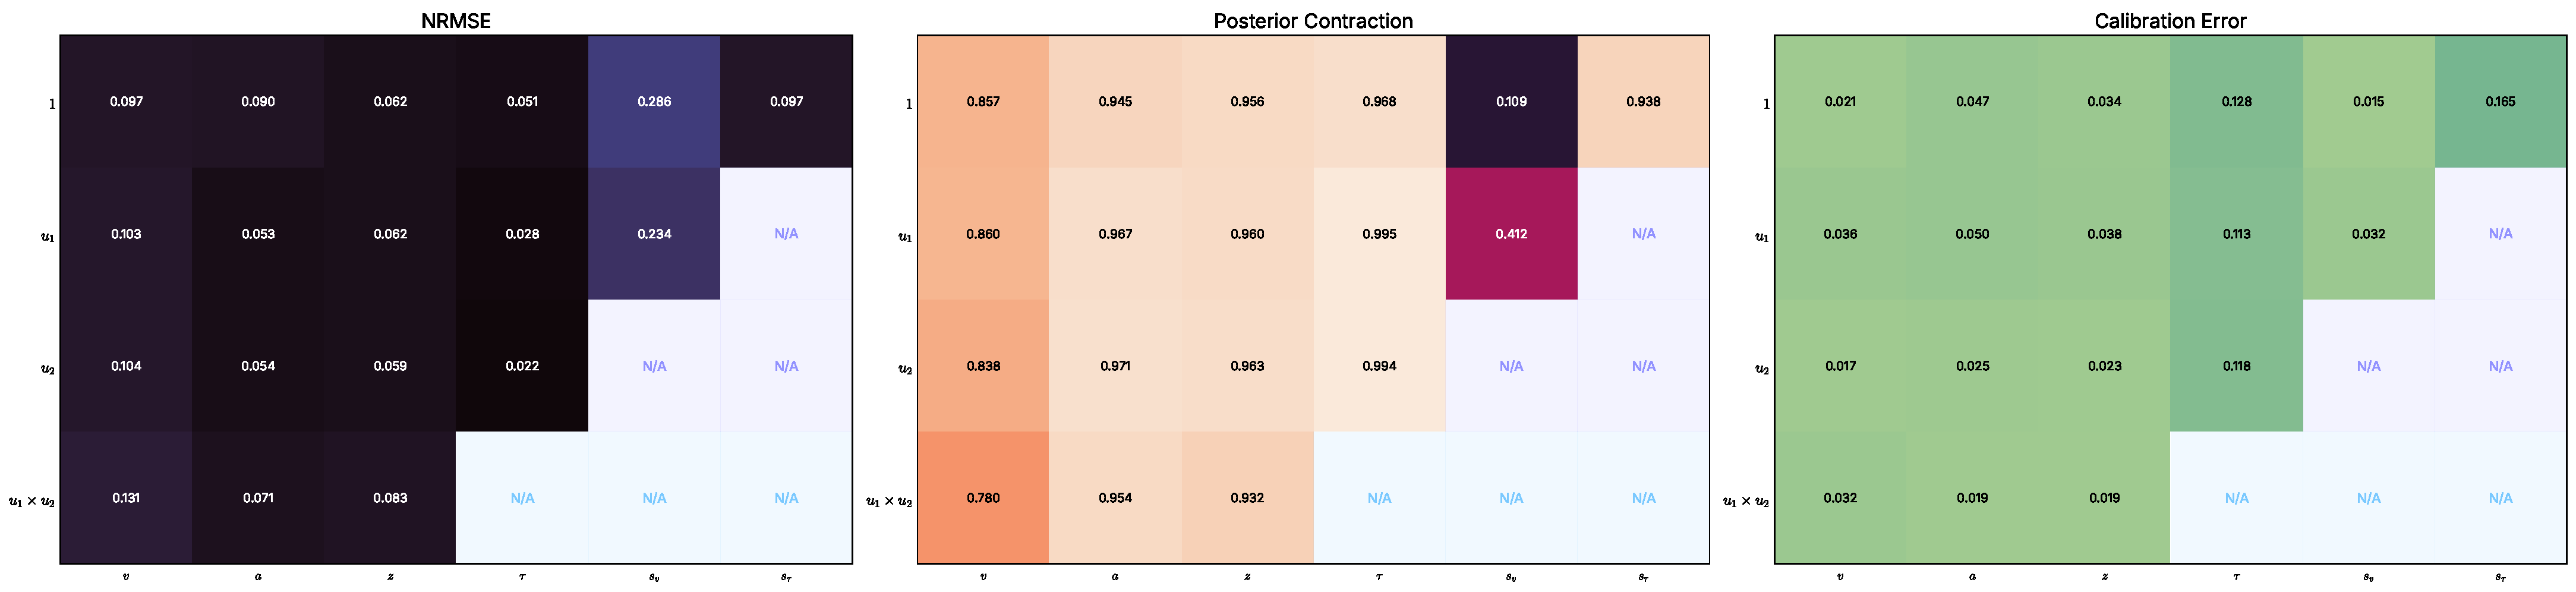
\includegraphics[width=\textwidth]{finetuned/ddm/interaction/metrics.pdf}
    \caption{Metrics}
  \end{subfigure}
  \caption{\textbf{After fine-tuning: DDM, \emph{interaction} design.} (a) Recovery, (b) calibration, (c) metrics. $v$, $a$, $z$, $\tau$ and $s_v$ carry slopes on $u_1$; $v$, $a$, $z$ and $\tau$ carry slopes on $u_2$; $v$, $a$ and $z$ on the product $u_1 u_2$ (18 coefficients shown). As in Figure~\ref{fig:app3-finetuned-lba-intercept-only}; before fine-tuning: Figure~\ref{fig:app1-ddm-interaction-cf}.}
  \label{fig:app3-finetuned-ddm-interaction}
\end{figure}

\begin{figure}[p]
  \centering
  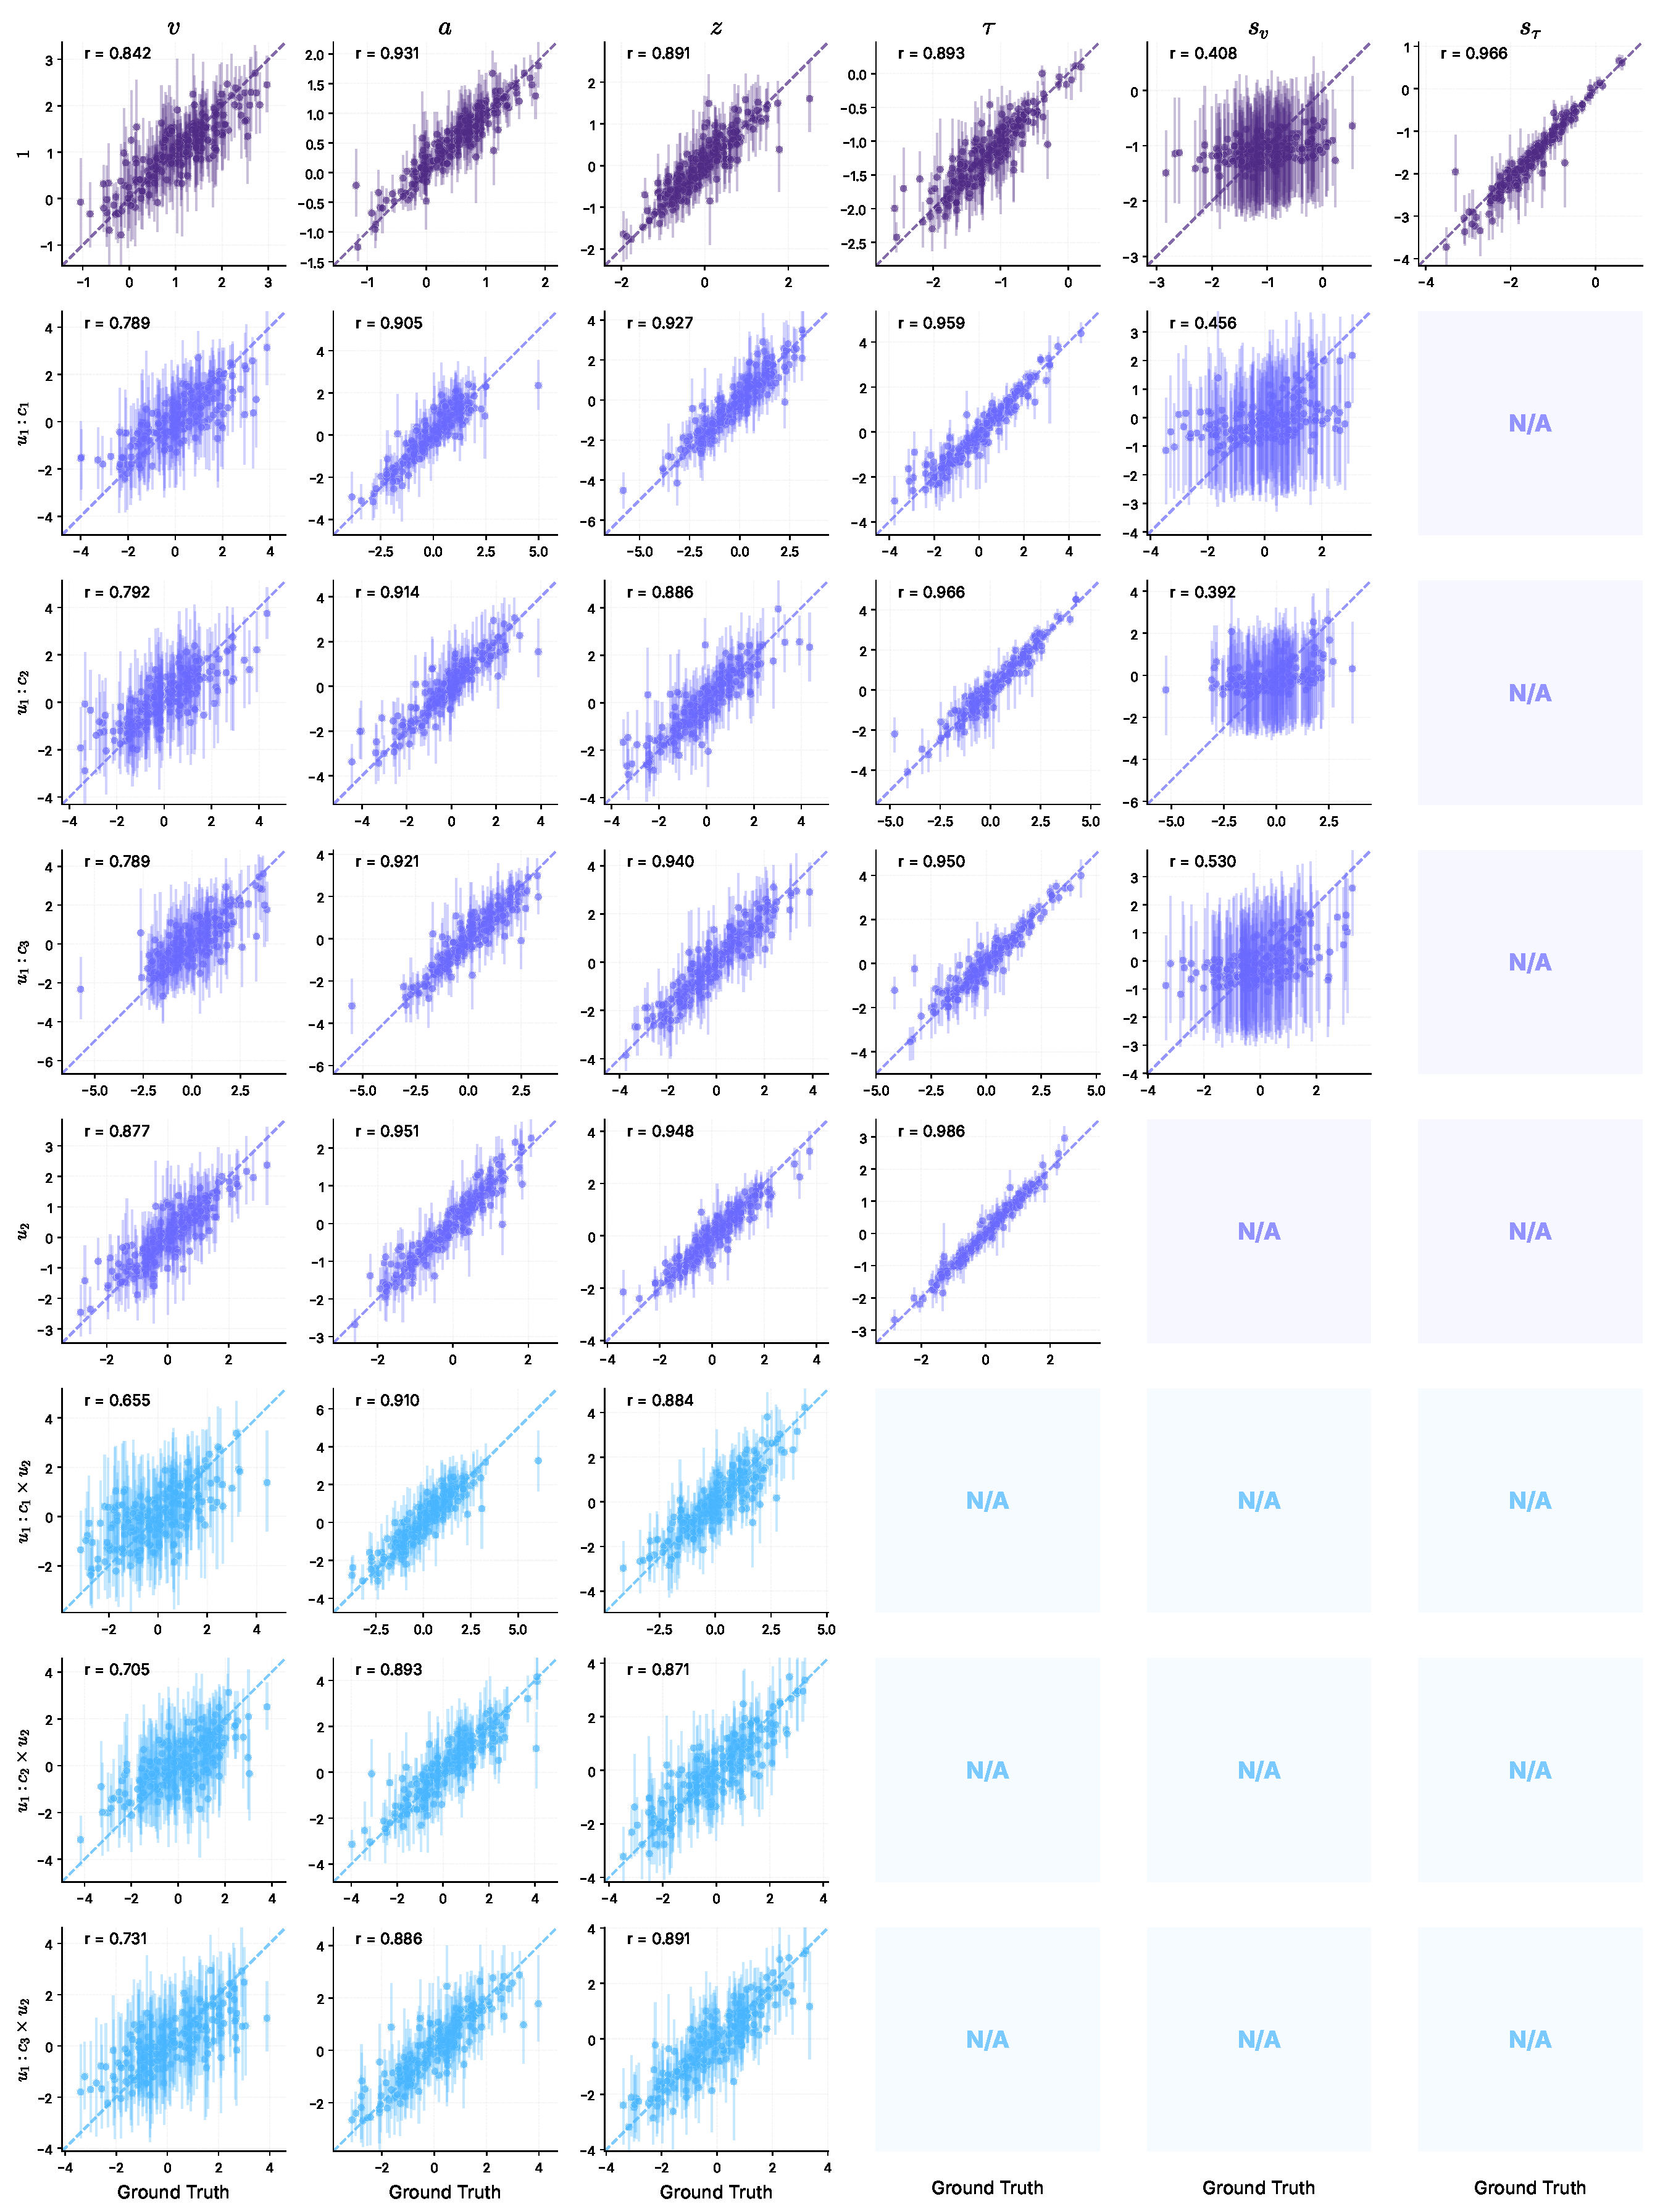
\includegraphics[width=\textwidth,height=0.82\textheight,keepaspectratio]{finetuned/ddm/mixed_predictor/recovery.pdf}
  \caption{\textbf{Parameter recovery, DDM after fine-tuning, mixed-predictor design.} $v$, $a$, $z$, $\tau$ and $s_v$ carry effects of the four-level $u_1$; $v$, $a$, $z$ and $\tau$ slopes on $u_2$; $v$, $a$ and $z$ the interaction (34 coefficients shown). Datasets simulated for this design (no shared benchmark file exists); design as in Figure~\ref{fig:app1-ddm-mixed-predictor-recovery}, encoding as in the top panel of Figure~\ref{fig:app1-ddm-intercept-only-cf}.}
  \label{fig:app3-finetuned-ddm-mixed-predictor-recovery}
\end{figure}

\begin{figure}[p]
  \centering
  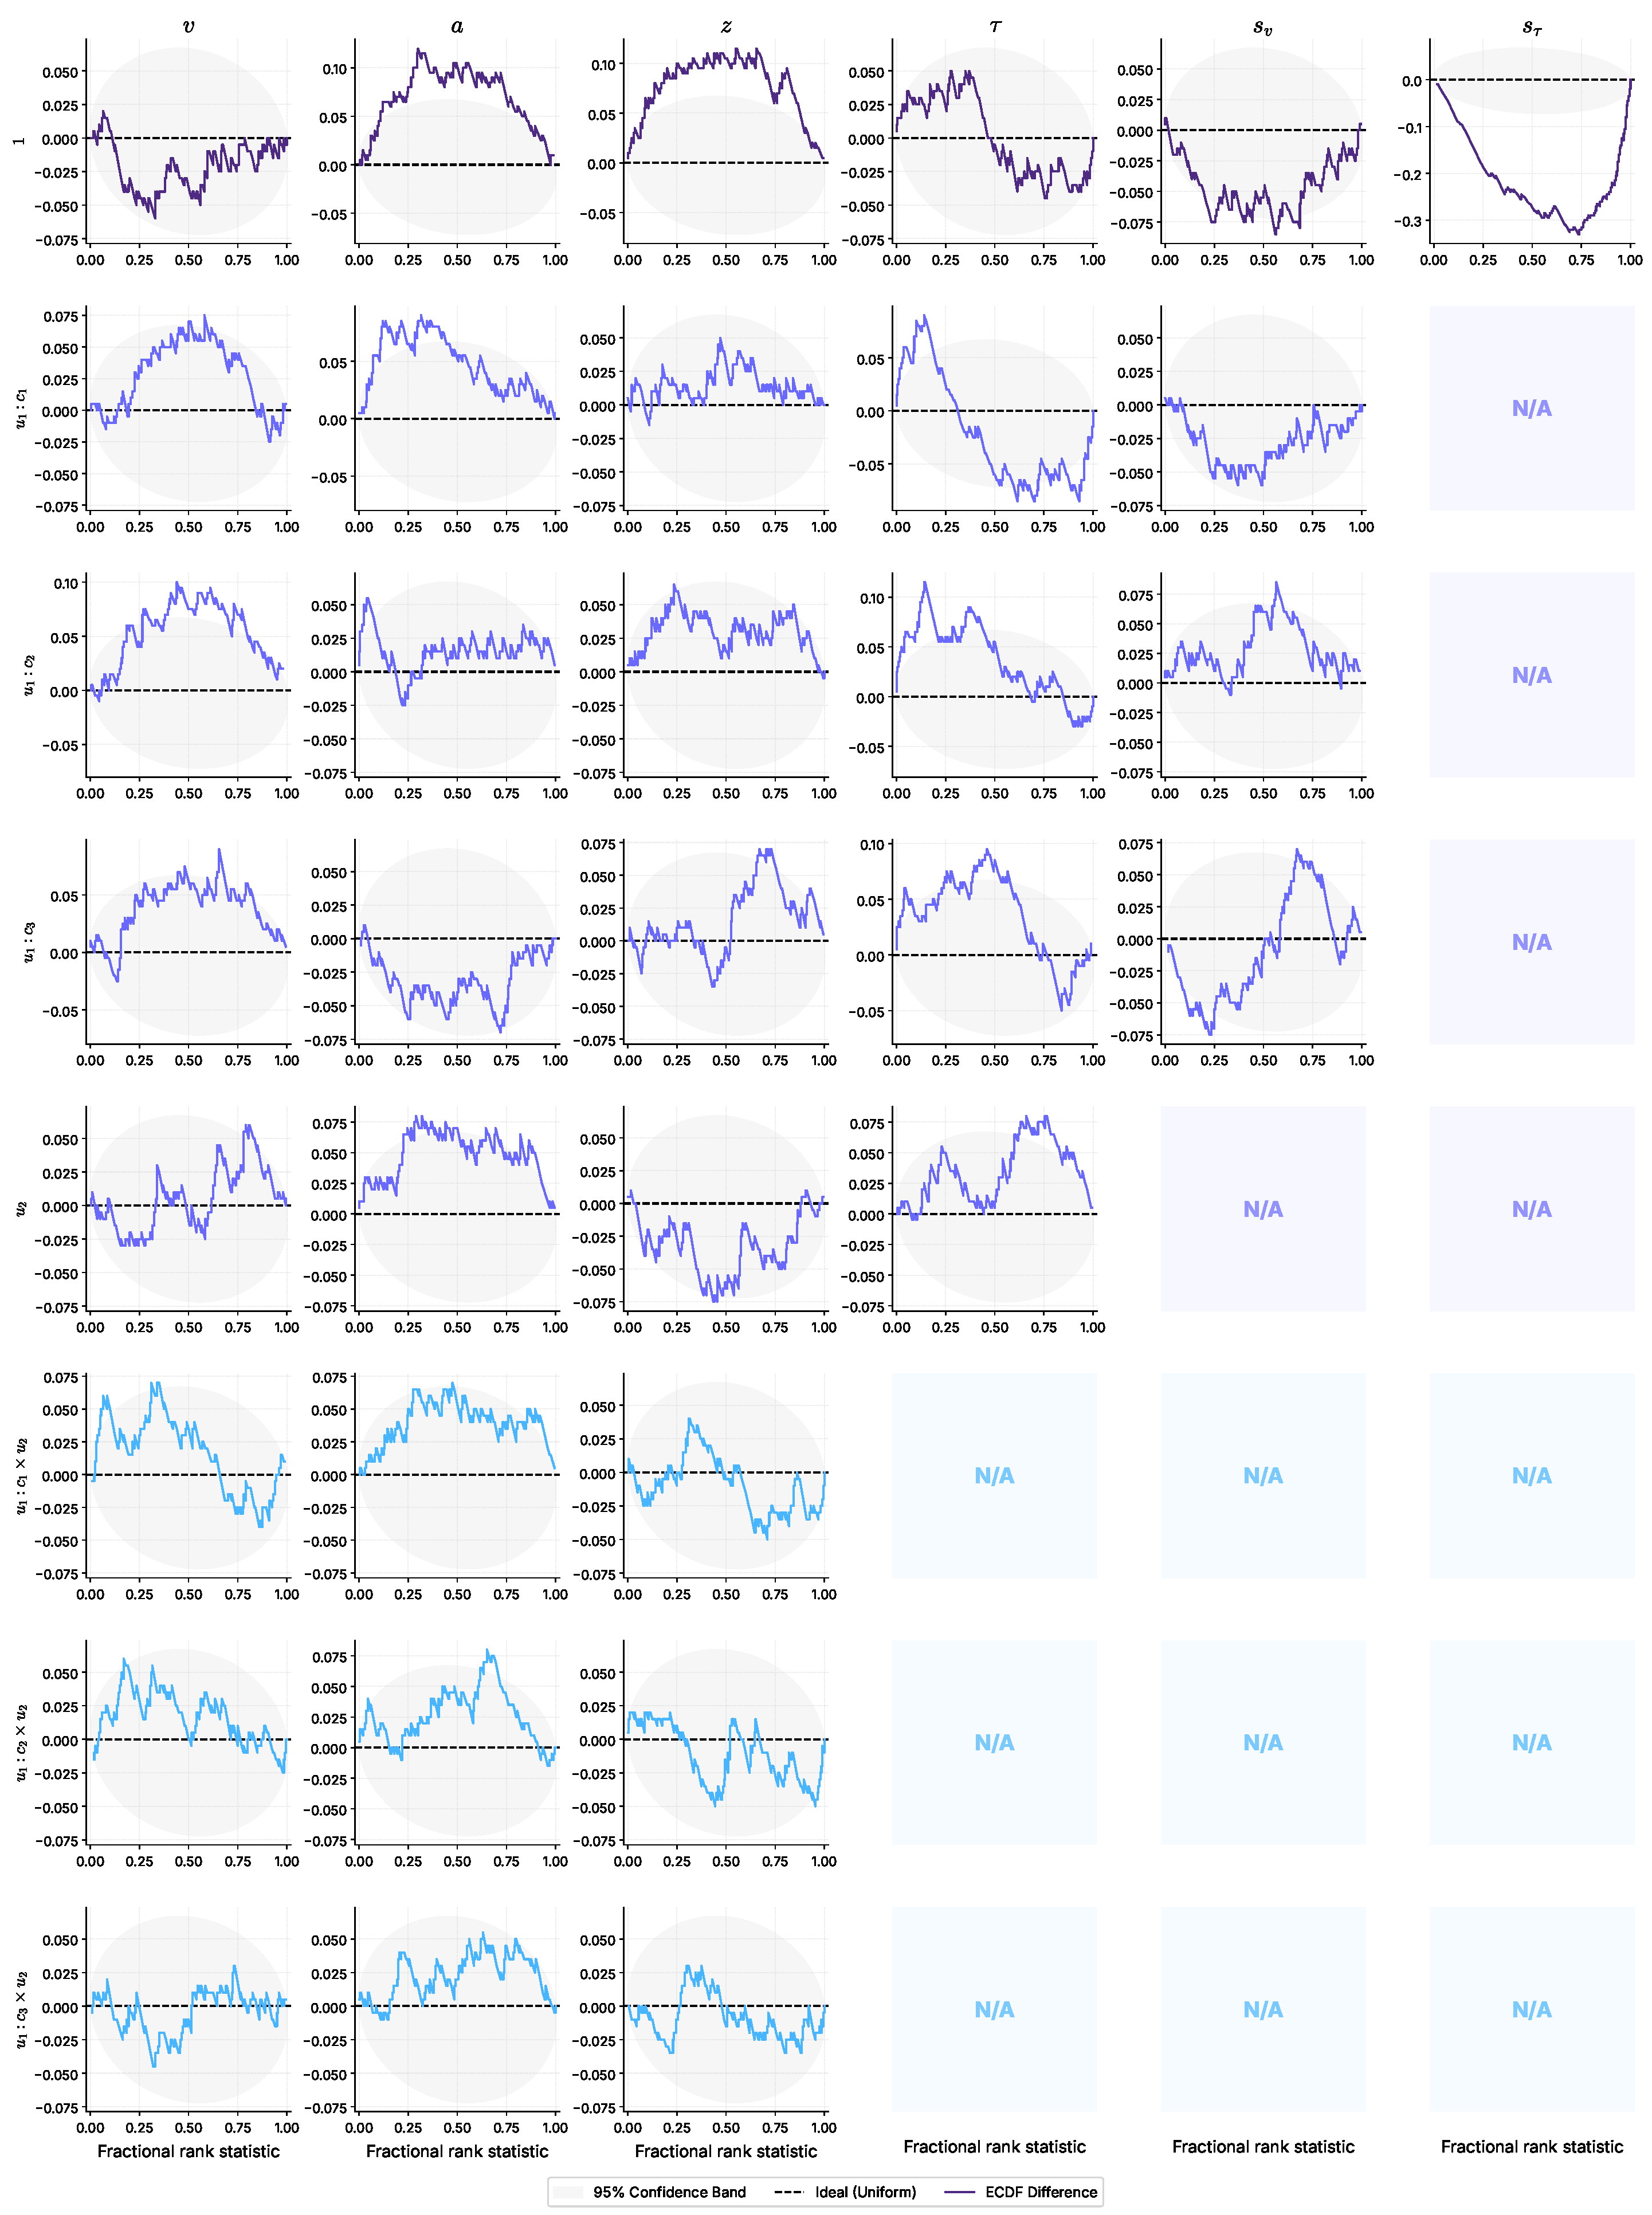
\includegraphics[width=\textwidth,height=0.82\textheight,keepaspectratio]{finetuned/ddm/mixed_predictor/ecdf.pdf}
  \caption{\textbf{Simulation-based calibration, DDM after fine-tuning, mixed-predictor design.} $v$, $a$, $z$, $\tau$ and $s_v$ carry effects of the four-level $u_1$; $v$, $a$, $z$ and $\tau$ slopes on $u_2$; $v$, $a$ and $z$ the interaction (34 coefficients shown). Datasets simulated for this design (no shared benchmark file exists); design as in Figure~\ref{fig:app1-ddm-mixed-predictor-recovery}, encoding as in the middle panel of Figure~\ref{fig:app1-ddm-intercept-only-cf}.}
  \label{fig:app3-finetuned-ddm-mixed-predictor-ecdf}
\end{figure}

\begin{figure}[p]
  \centering
  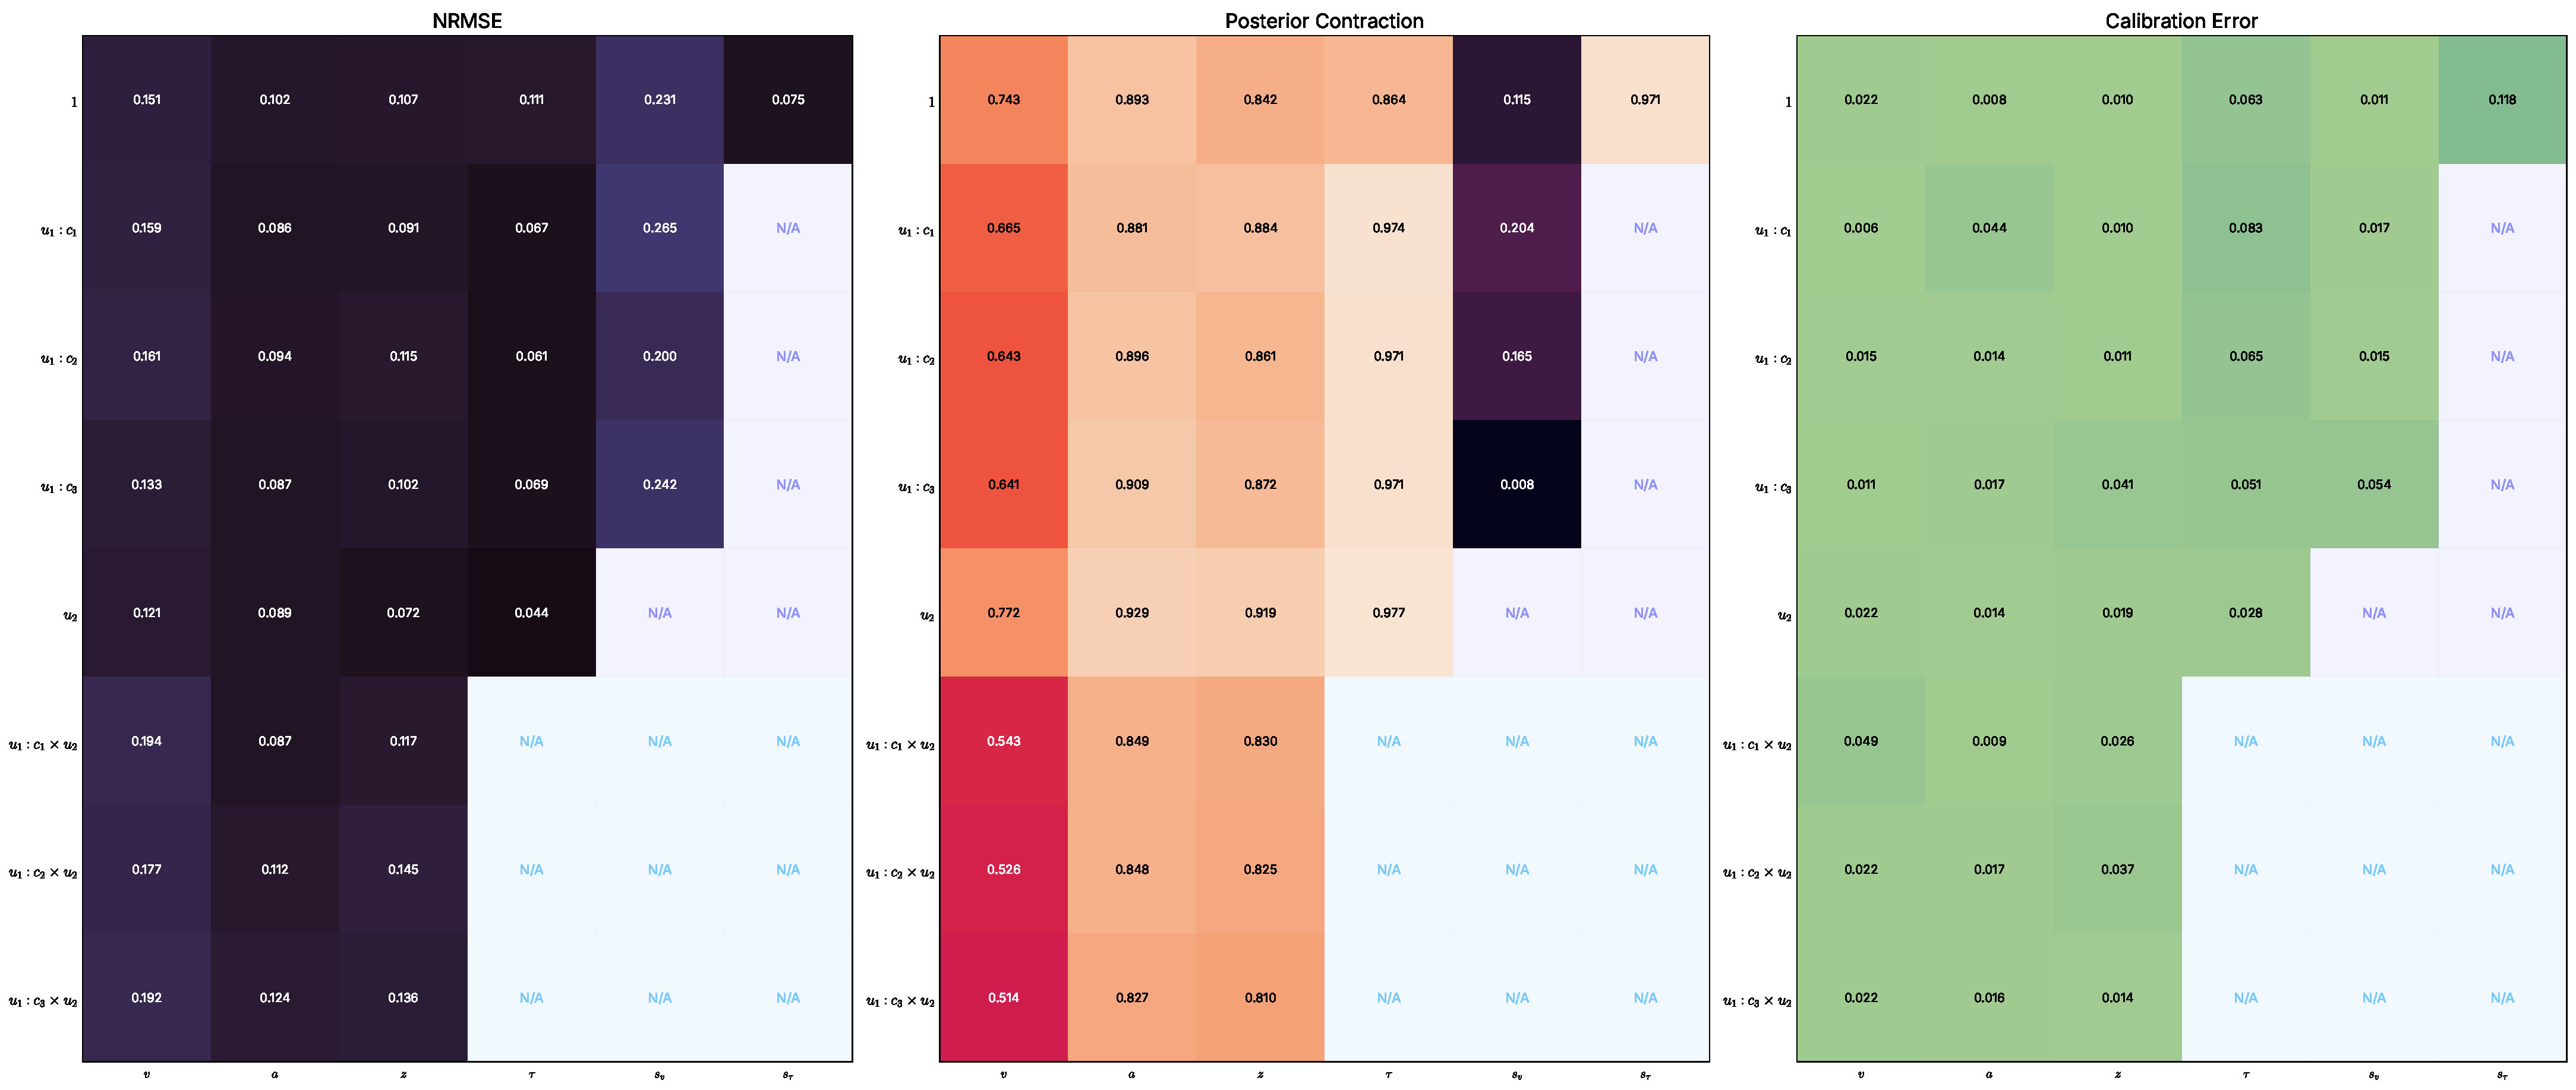
\includegraphics[width=\textwidth,height=0.82\textheight,keepaspectratio]{finetuned/ddm/mixed_predictor/metrics.pdf}
  \caption{\textbf{Summary metrics, DDM after fine-tuning, mixed-predictor design.} $v$, $a$, $z$, $\tau$ and $s_v$ carry effects of the four-level $u_1$; $v$, $a$, $z$ and $\tau$ slopes on $u_2$; $v$, $a$ and $z$ the interaction (34 coefficients shown). Datasets simulated for this design (no shared benchmark file exists); design as in Figure~\ref{fig:app1-ddm-mixed-predictor-recovery}, encoding as in the bottom panel of Figure~\ref{fig:app1-ddm-intercept-only-cf}.}
  \label{fig:app3-finetuned-ddm-mixed-predictor-metrics}
\end{figure}

\begin{figure}[p]
  \centering
  \begin{subfigure}{\textwidth}\centering
    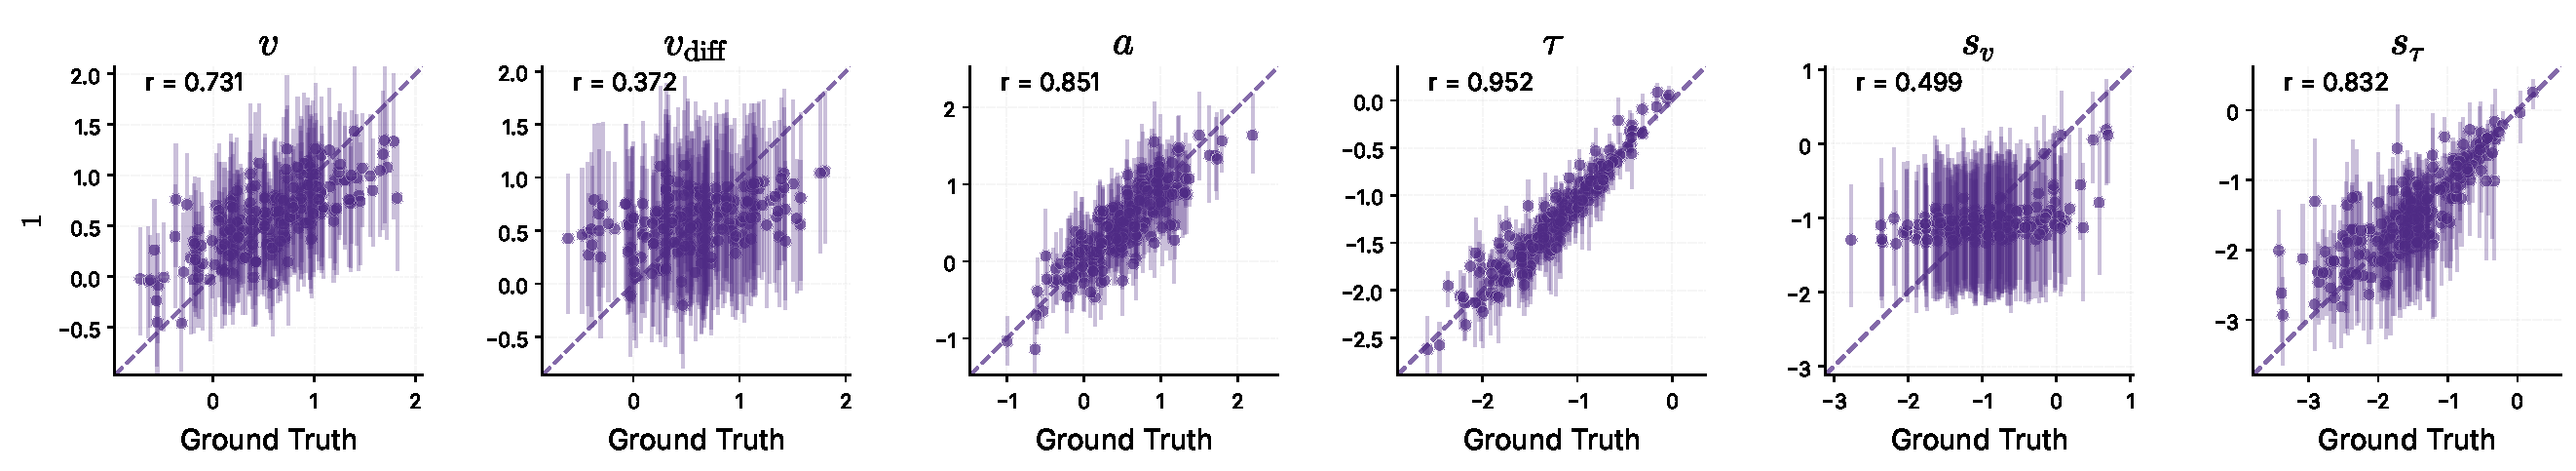
\includegraphics[width=\textwidth,height=0.3\textheight,keepaspectratio]{finetuned/rdm/intercept_only/recovery.pdf}
    \caption{Recovery}
  \end{subfigure}\\[1ex]
  \begin{subfigure}{\textwidth}\centering
    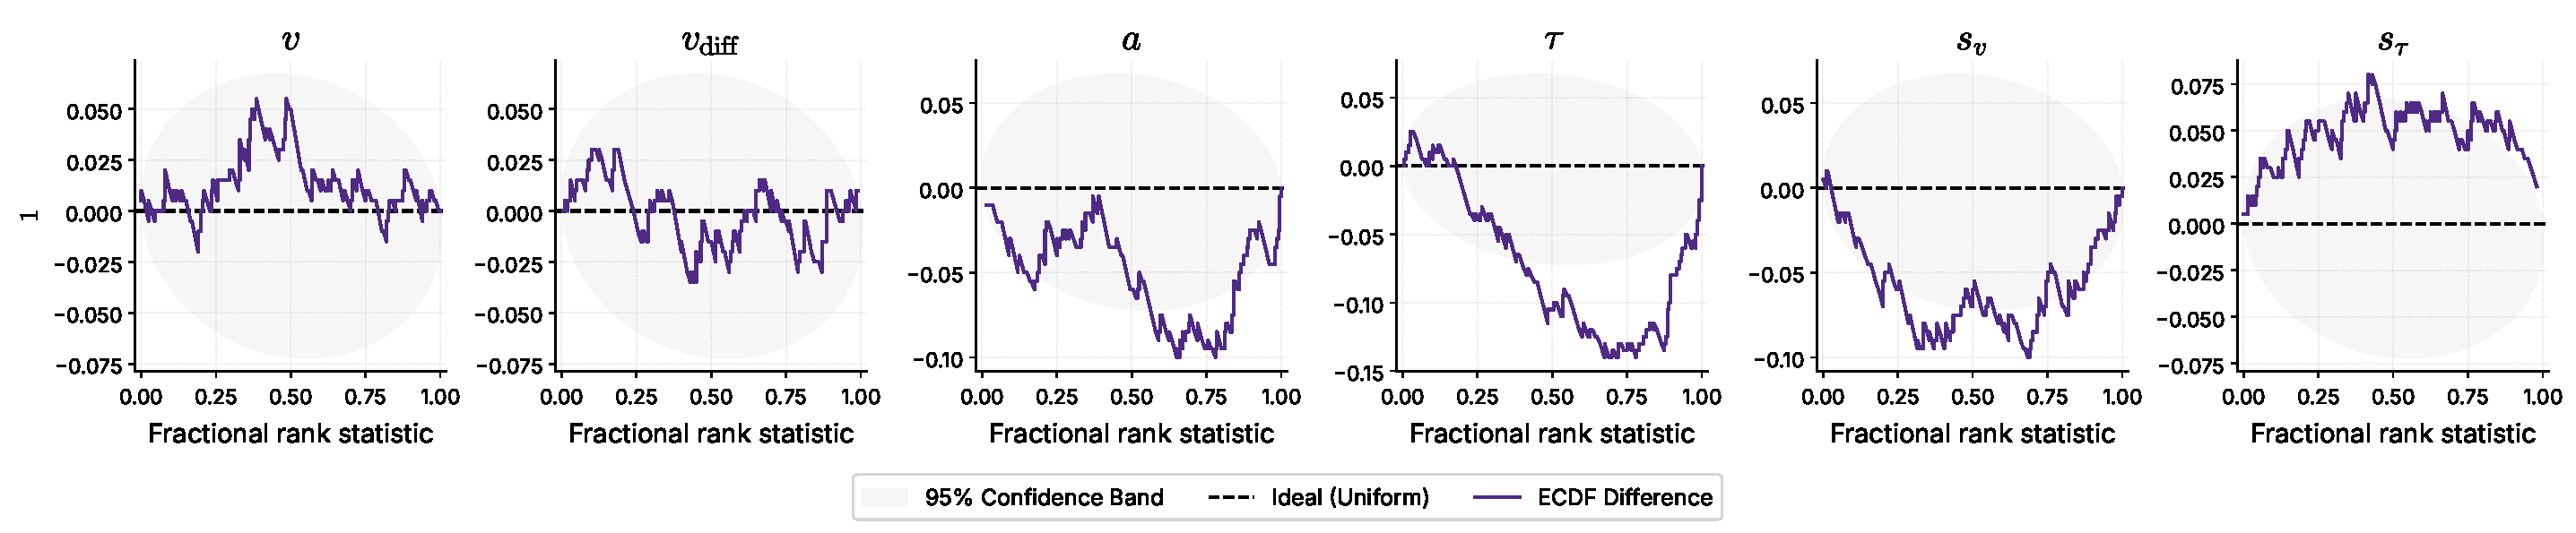
\includegraphics[width=\textwidth,height=0.3\textheight,keepaspectratio]{finetuned/rdm/intercept_only/ecdf.pdf}
    \caption{Calibration (ECDF)}
  \end{subfigure}\\[1ex]
  \begin{subfigure}{\textwidth}\centering
    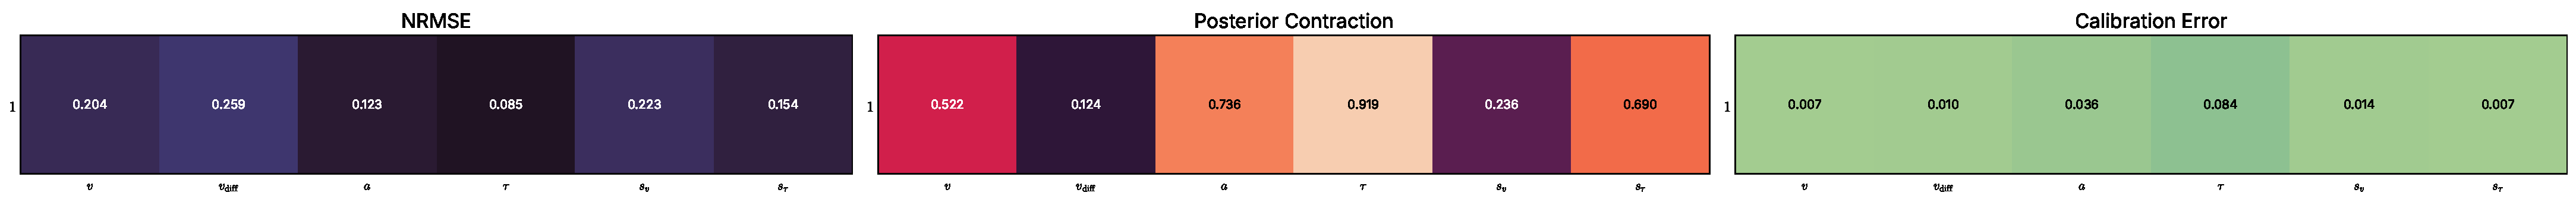
\includegraphics[width=\textwidth]{finetuned/rdm/intercept_only/metrics.pdf}
    \caption{Metrics}
  \end{subfigure}
  \caption{\textbf{After fine-tuning: RDM, \emph{intercept-only} design.} (a) Recovery, (b) calibration, (c) metrics. Every estimated parameter enters as an intercept only (6 coefficients shown). As in Figure~\ref{fig:app3-finetuned-lba-intercept-only}; before fine-tuning: Figure~\ref{fig:app1-rdm-intercept-only-cf}.}
  \label{fig:app3-finetuned-rdm-intercept-only}
\end{figure}

\begin{figure}[p]
  \centering
  \begin{subfigure}{\textwidth}\centering
    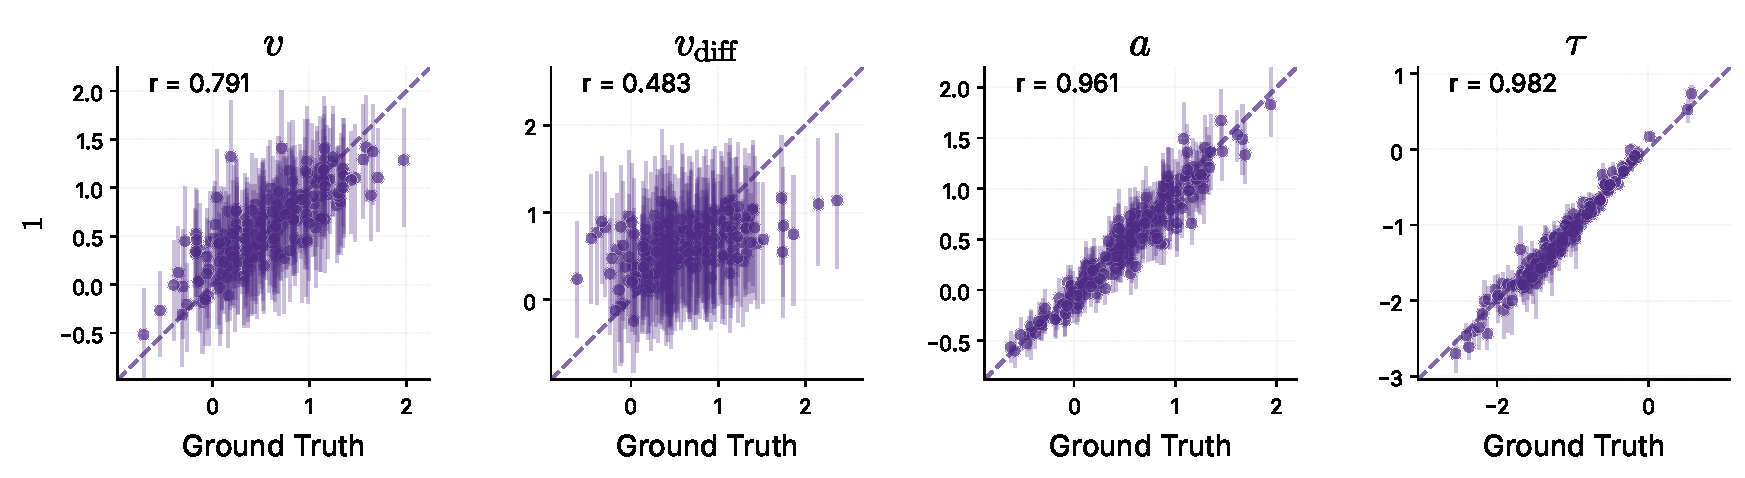
\includegraphics[width=\textwidth,height=0.3\textheight,keepaspectratio]{finetuned/rdm/fixed/recovery.pdf}
    \caption{Recovery}
  \end{subfigure}\\[1ex]
  \begin{subfigure}{\textwidth}\centering
    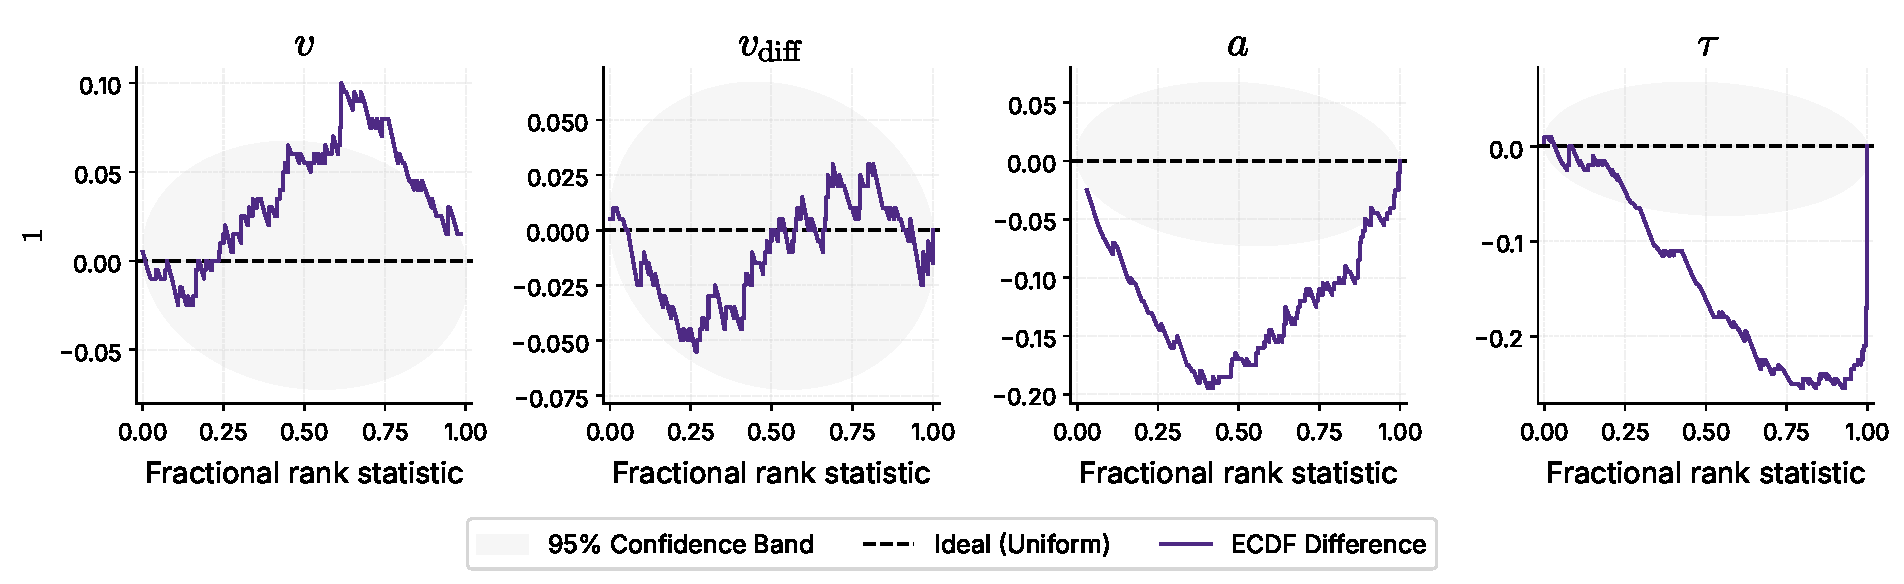
\includegraphics[width=\textwidth,height=0.3\textheight,keepaspectratio]{finetuned/rdm/fixed/ecdf.pdf}
    \caption{Calibration (ECDF)}
  \end{subfigure}\\[1ex]
  \begin{subfigure}{\textwidth}\centering
    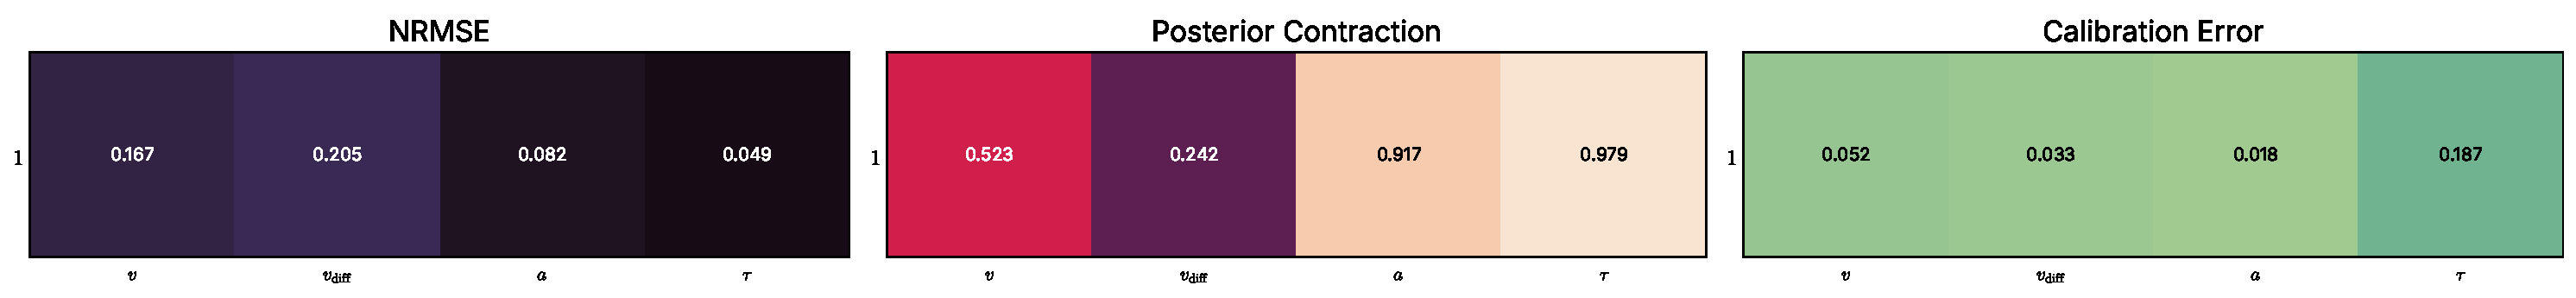
\includegraphics[width=\textwidth]{finetuned/rdm/fixed/metrics.pdf}
    \caption{Metrics}
  \end{subfigure}
  \caption{\textbf{After fine-tuning: RDM, \emph{fixed} design.} (a) Recovery, (b) calibration, (c) metrics. $s_v$ and $s_\tau$ are fixed at 0 and not estimated; every estimated parameter enters as an intercept only (4 coefficients shown). As in Figure~\ref{fig:app3-finetuned-lba-intercept-only}; before fine-tuning: Figure~\ref{fig:app1-rdm-fixed-cf}.}
  \label{fig:app3-finetuned-rdm-fixed}
\end{figure}

\begin{figure}[p]
  \centering
  \begin{subfigure}{\textwidth}\centering
    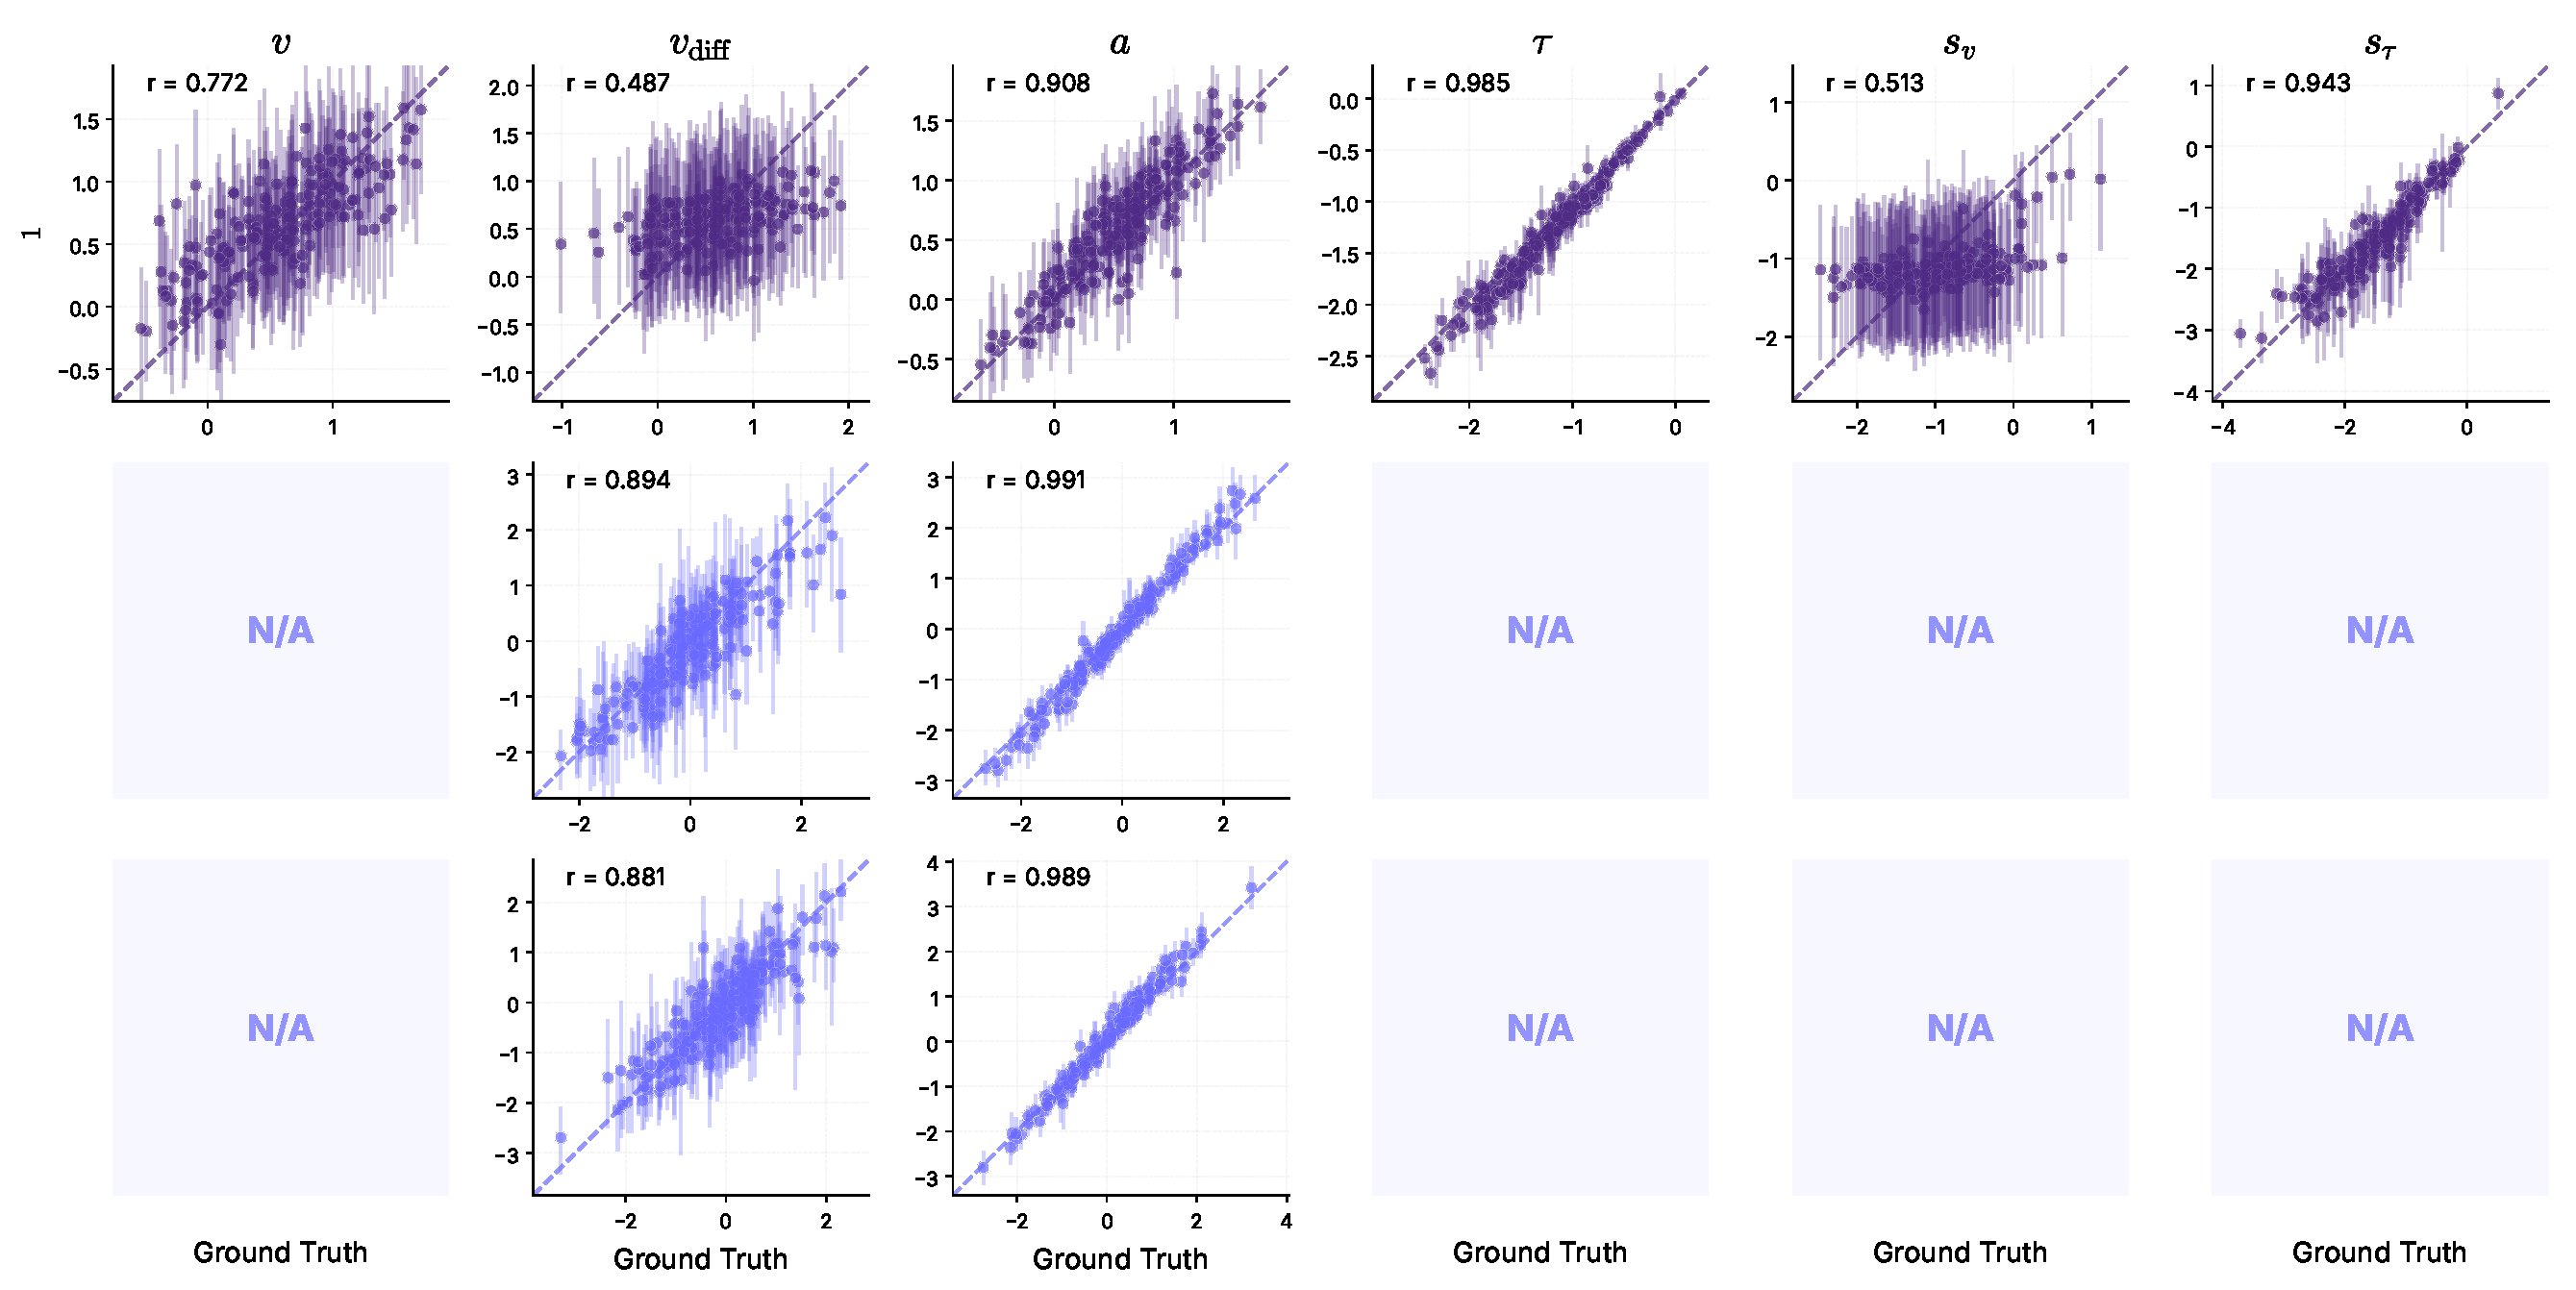
\includegraphics[width=\textwidth,height=0.3\textheight,keepaspectratio]{finetuned/rdm/regressed/recovery.pdf}
    \caption{Recovery}
  \end{subfigure}\\[1ex]
  \begin{subfigure}{\textwidth}\centering
    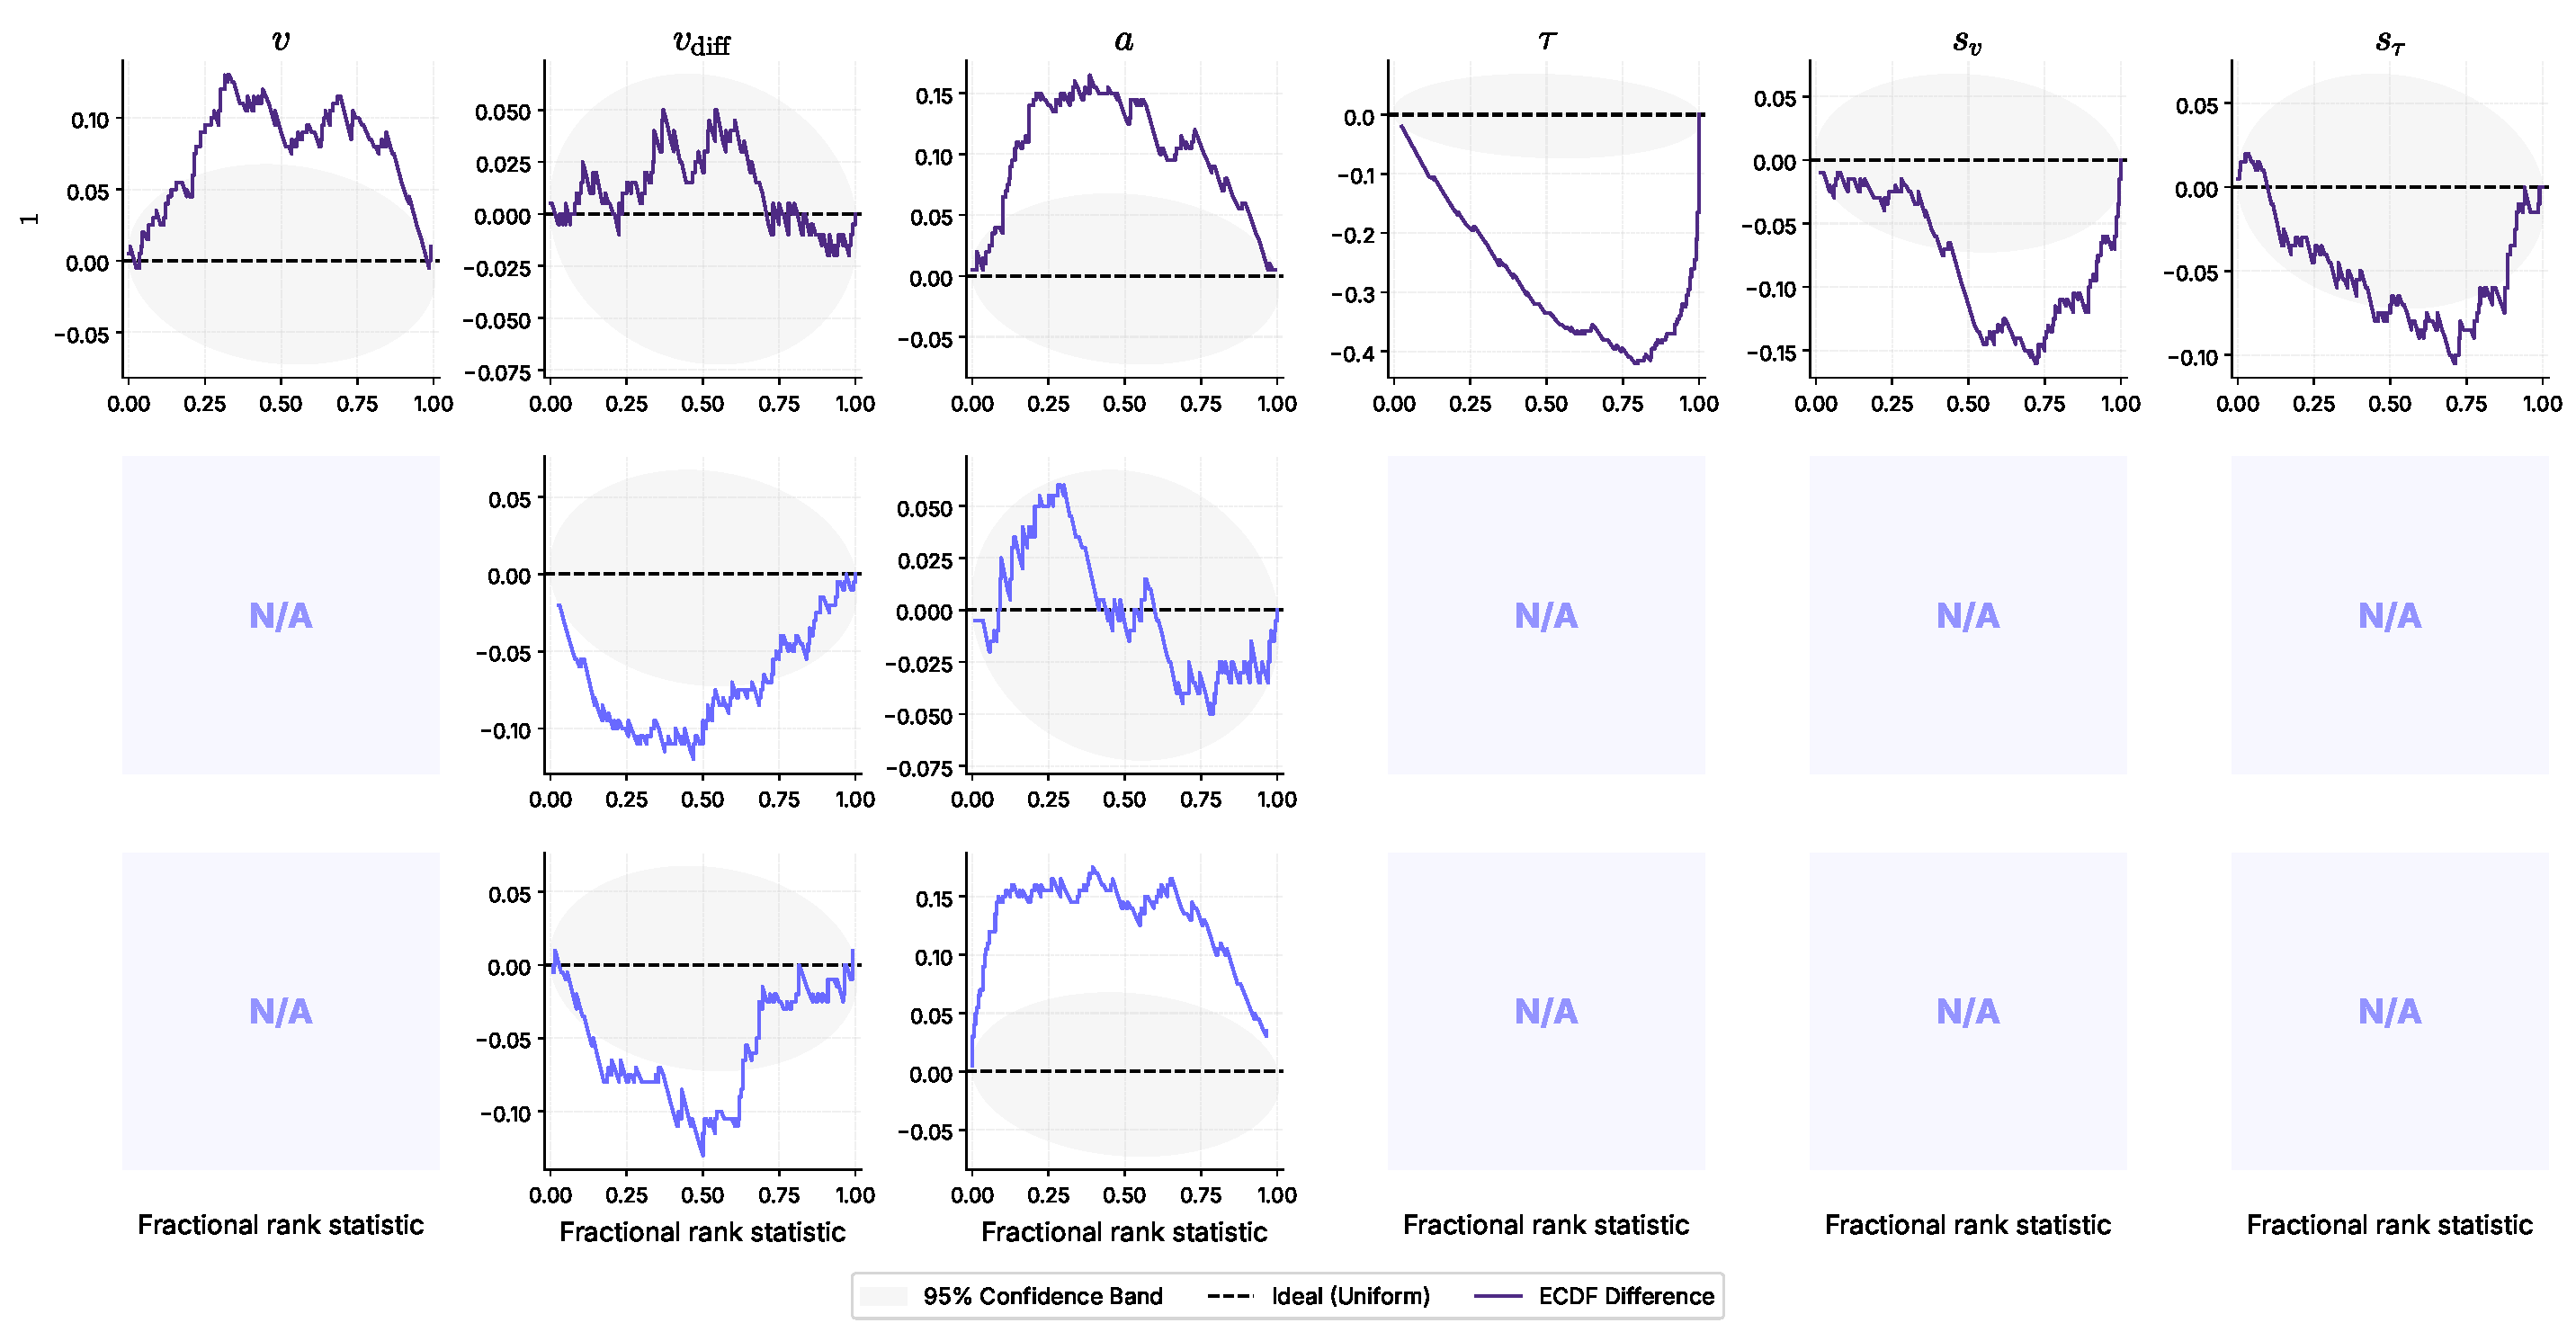
\includegraphics[width=\textwidth,height=0.3\textheight,keepaspectratio]{finetuned/rdm/regressed/ecdf.pdf}
    \caption{Calibration (ECDF)}
  \end{subfigure}\\[1ex]
  \begin{subfigure}{\textwidth}\centering
    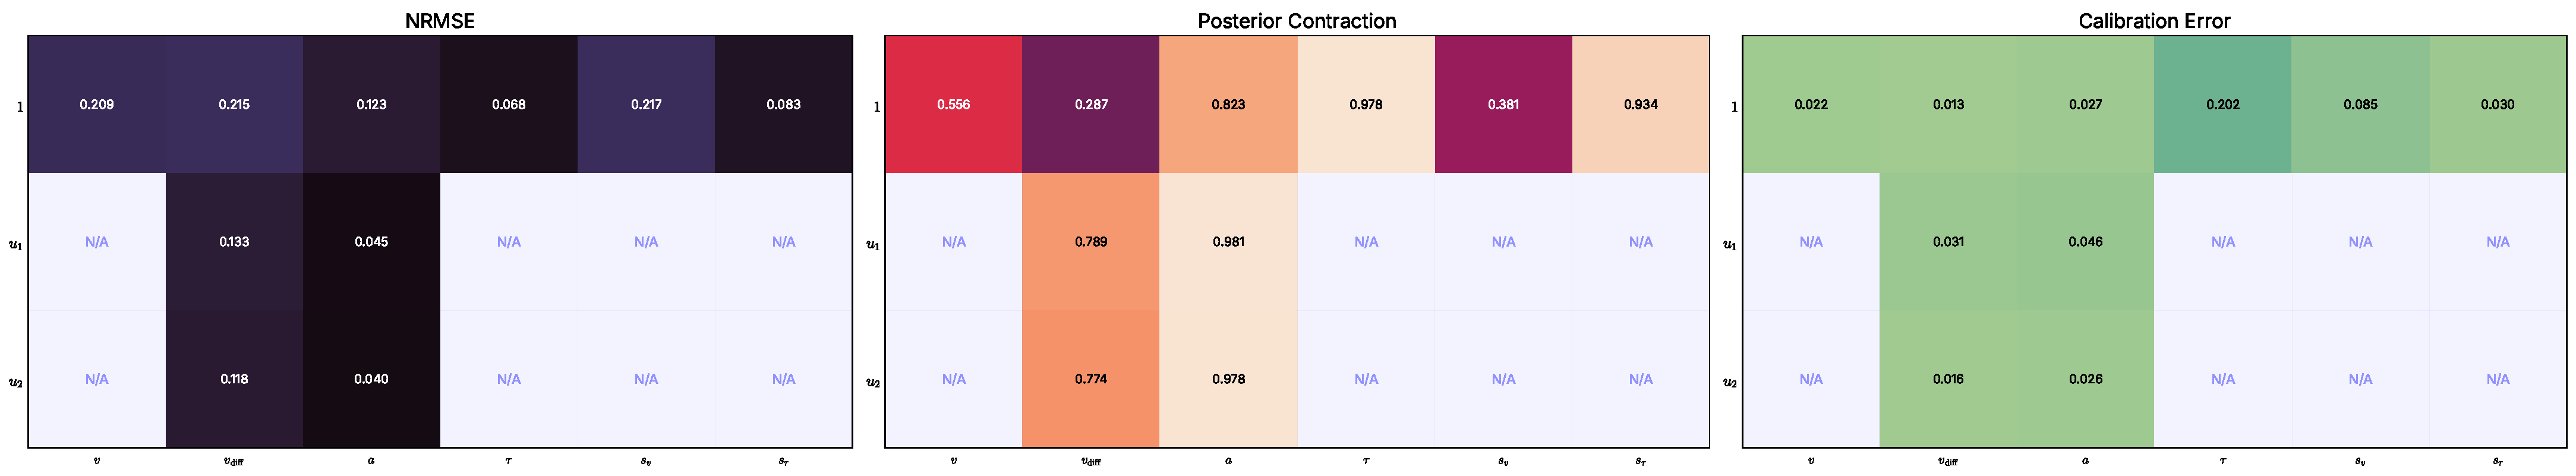
\includegraphics[width=\textwidth]{finetuned/rdm/regressed/metrics.pdf}
    \caption{Metrics}
  \end{subfigure}
  \caption{\textbf{After fine-tuning: RDM, \emph{regressed} design.} (a) Recovery, (b) calibration, (c) metrics. $v_{\mathrm{diff}}$ and $a$ carry slopes on $u_1$ and $u_2$ (10 coefficients shown). As in Figure~\ref{fig:app3-finetuned-lba-intercept-only}; before fine-tuning: Figure~\ref{fig:app1-rdm-regressed-cf}.}
  \label{fig:app3-finetuned-rdm-regressed}
\end{figure}

\begin{figure}[p]
  \centering
  \begin{subfigure}{\textwidth}\centering
    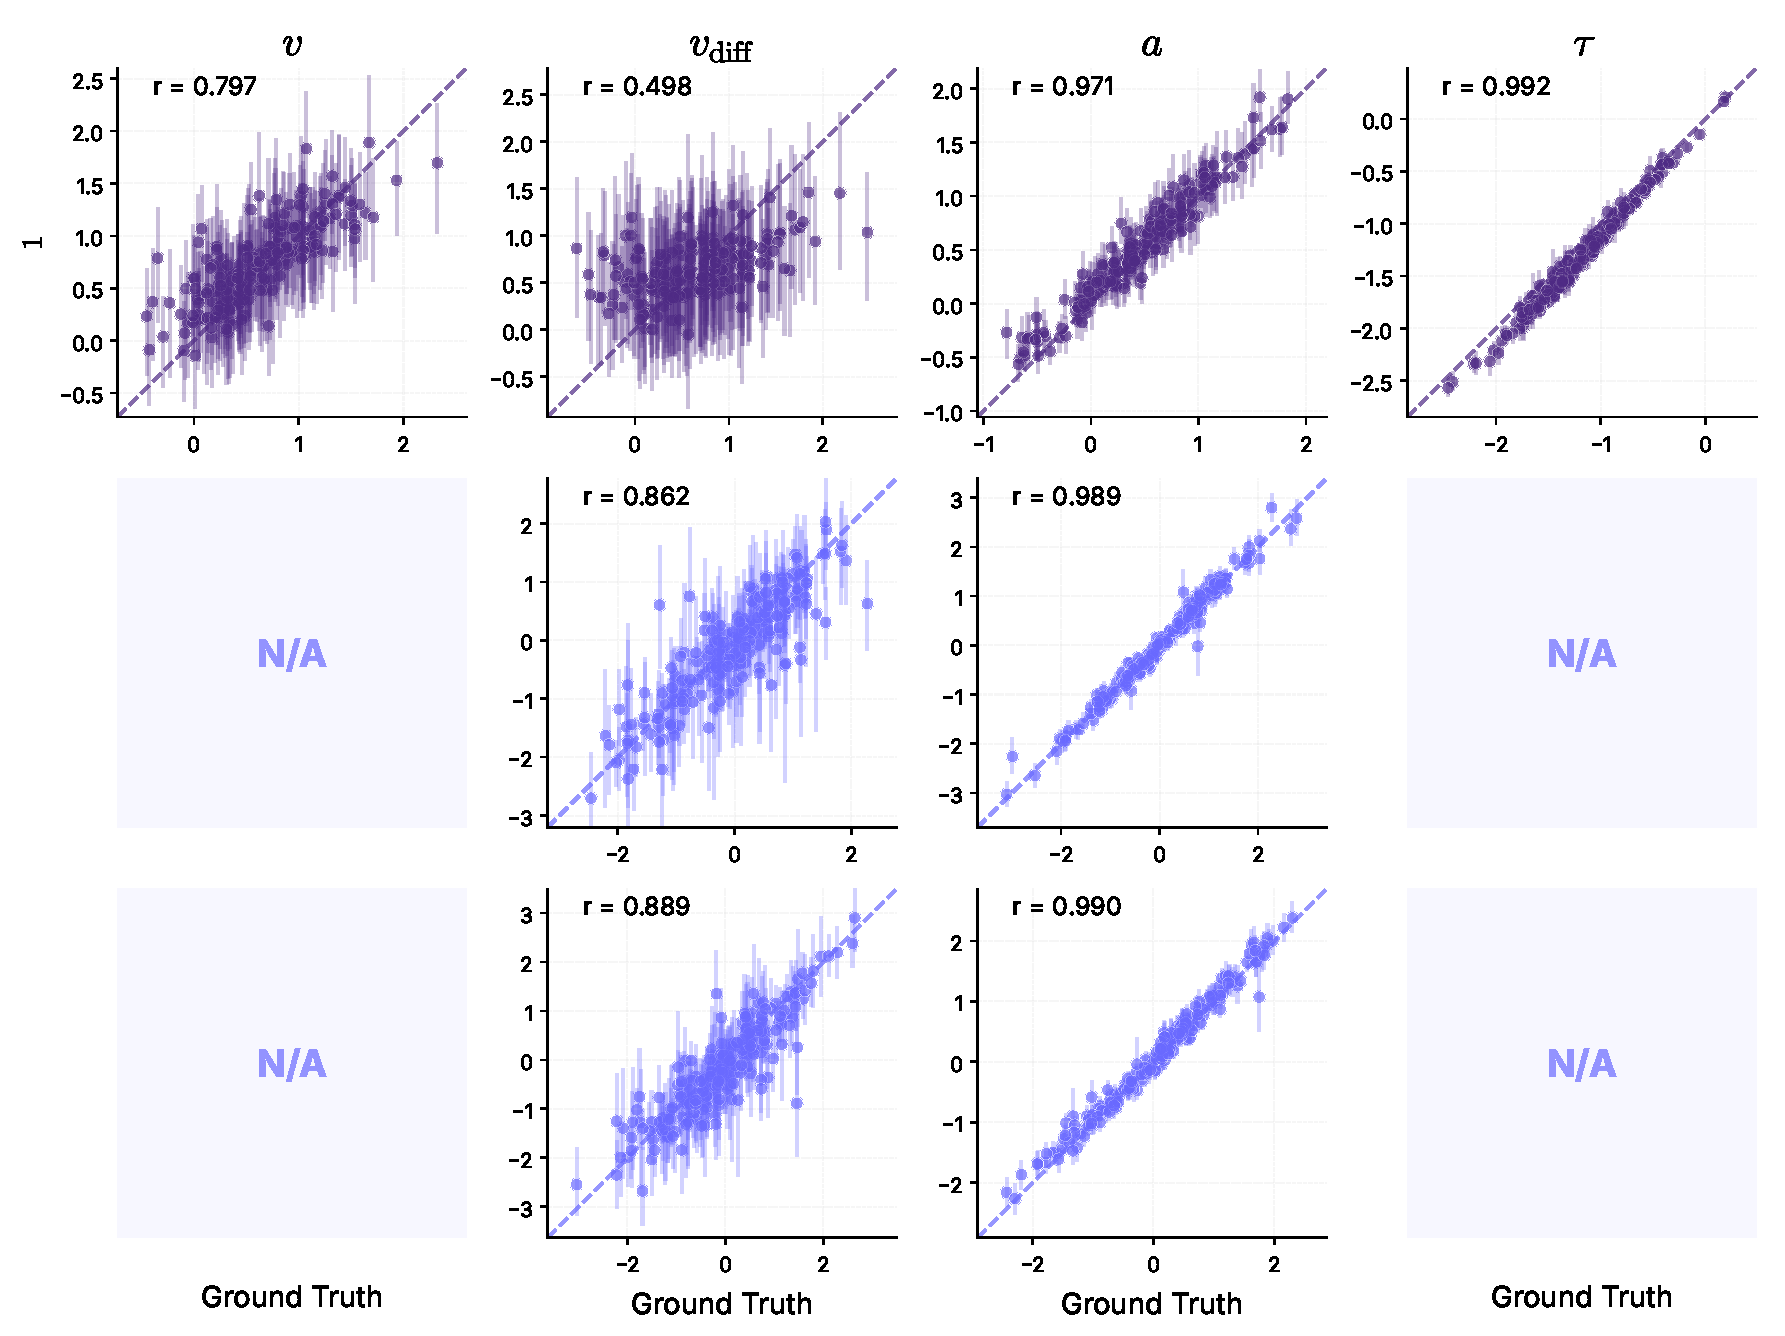
\includegraphics[width=\textwidth,height=0.3\textheight,keepaspectratio]{finetuned/rdm/fixed_regressed/recovery.pdf}
    \caption{Recovery}
  \end{subfigure}\\[1ex]
  \begin{subfigure}{\textwidth}\centering
    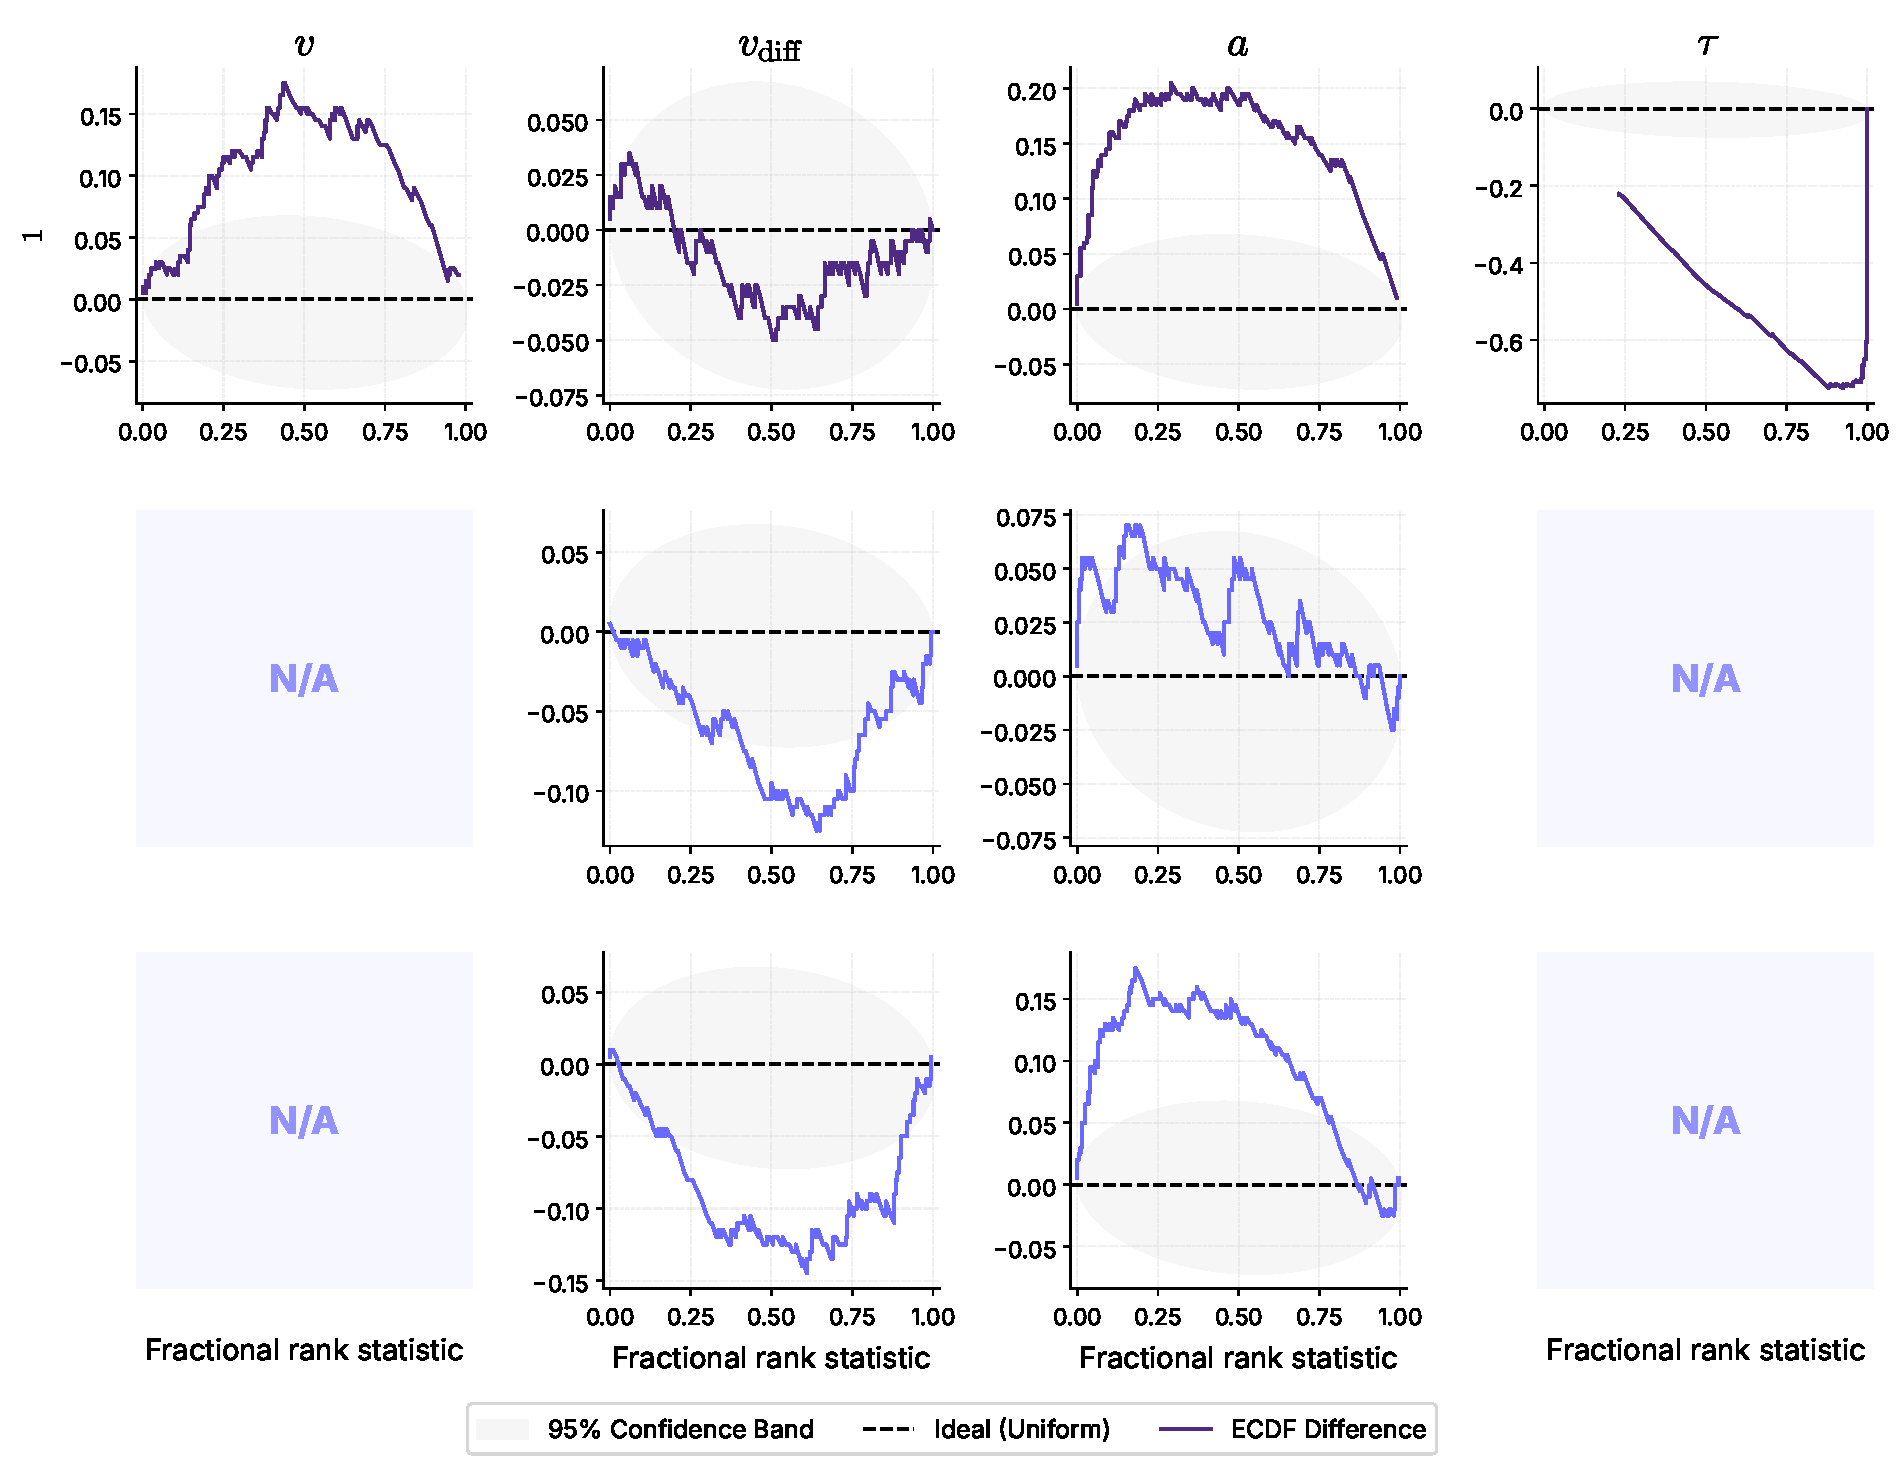
\includegraphics[width=\textwidth,height=0.3\textheight,keepaspectratio]{finetuned/rdm/fixed_regressed/ecdf.pdf}
    \caption{Calibration (ECDF)}
  \end{subfigure}\\[1ex]
  \begin{subfigure}{\textwidth}\centering
    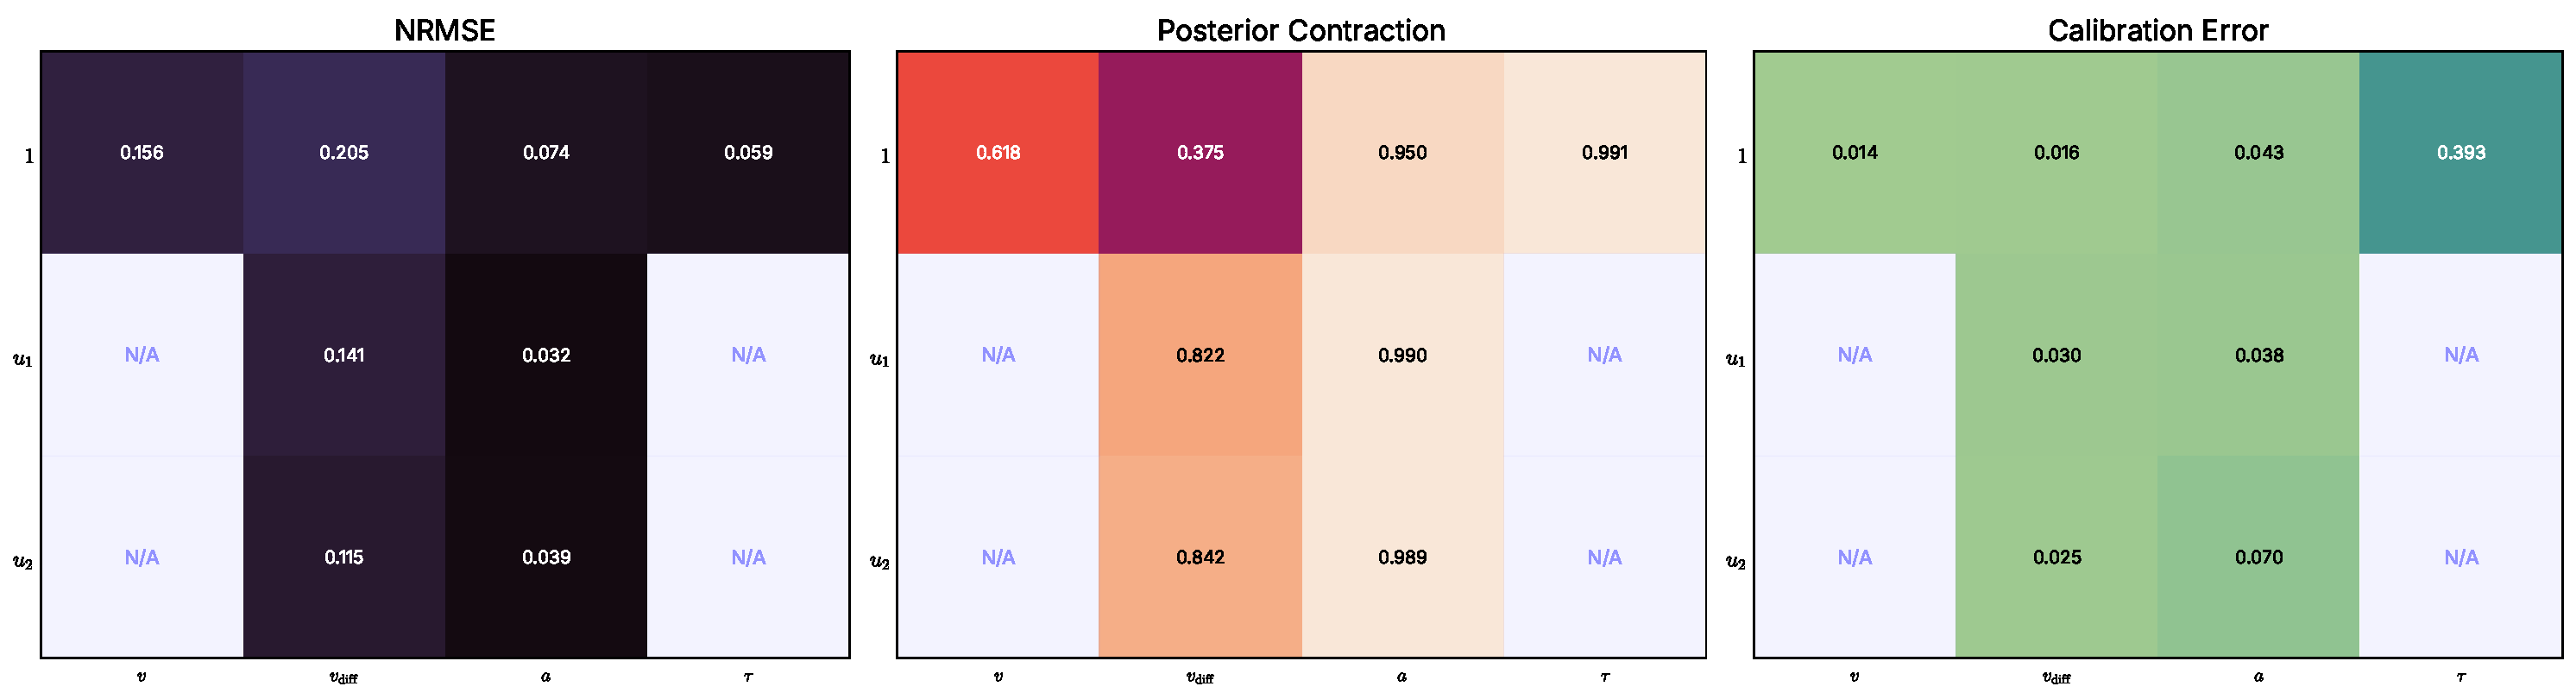
\includegraphics[width=\textwidth]{finetuned/rdm/fixed_regressed/metrics.pdf}
    \caption{Metrics}
  \end{subfigure}
  \caption{\textbf{After fine-tuning: RDM, \emph{fixed + regressed} design.} (a) Recovery, (b) calibration, (c) metrics. $s_v$ and $s_\tau$ are fixed at 0 and not estimated; $v_{\mathrm{diff}}$ and $a$ carry slopes on $u_1$ and $u_2$ (8 coefficients shown). As in Figure~\ref{fig:app3-finetuned-lba-intercept-only}; before fine-tuning: Figure~\ref{fig:app1-rdm-fixed-regressed-cf}.}
  \label{fig:app3-finetuned-rdm-fixed-regressed}
\end{figure}

\begin{figure}[p]
  \centering
  \begin{subfigure}{\textwidth}\centering
    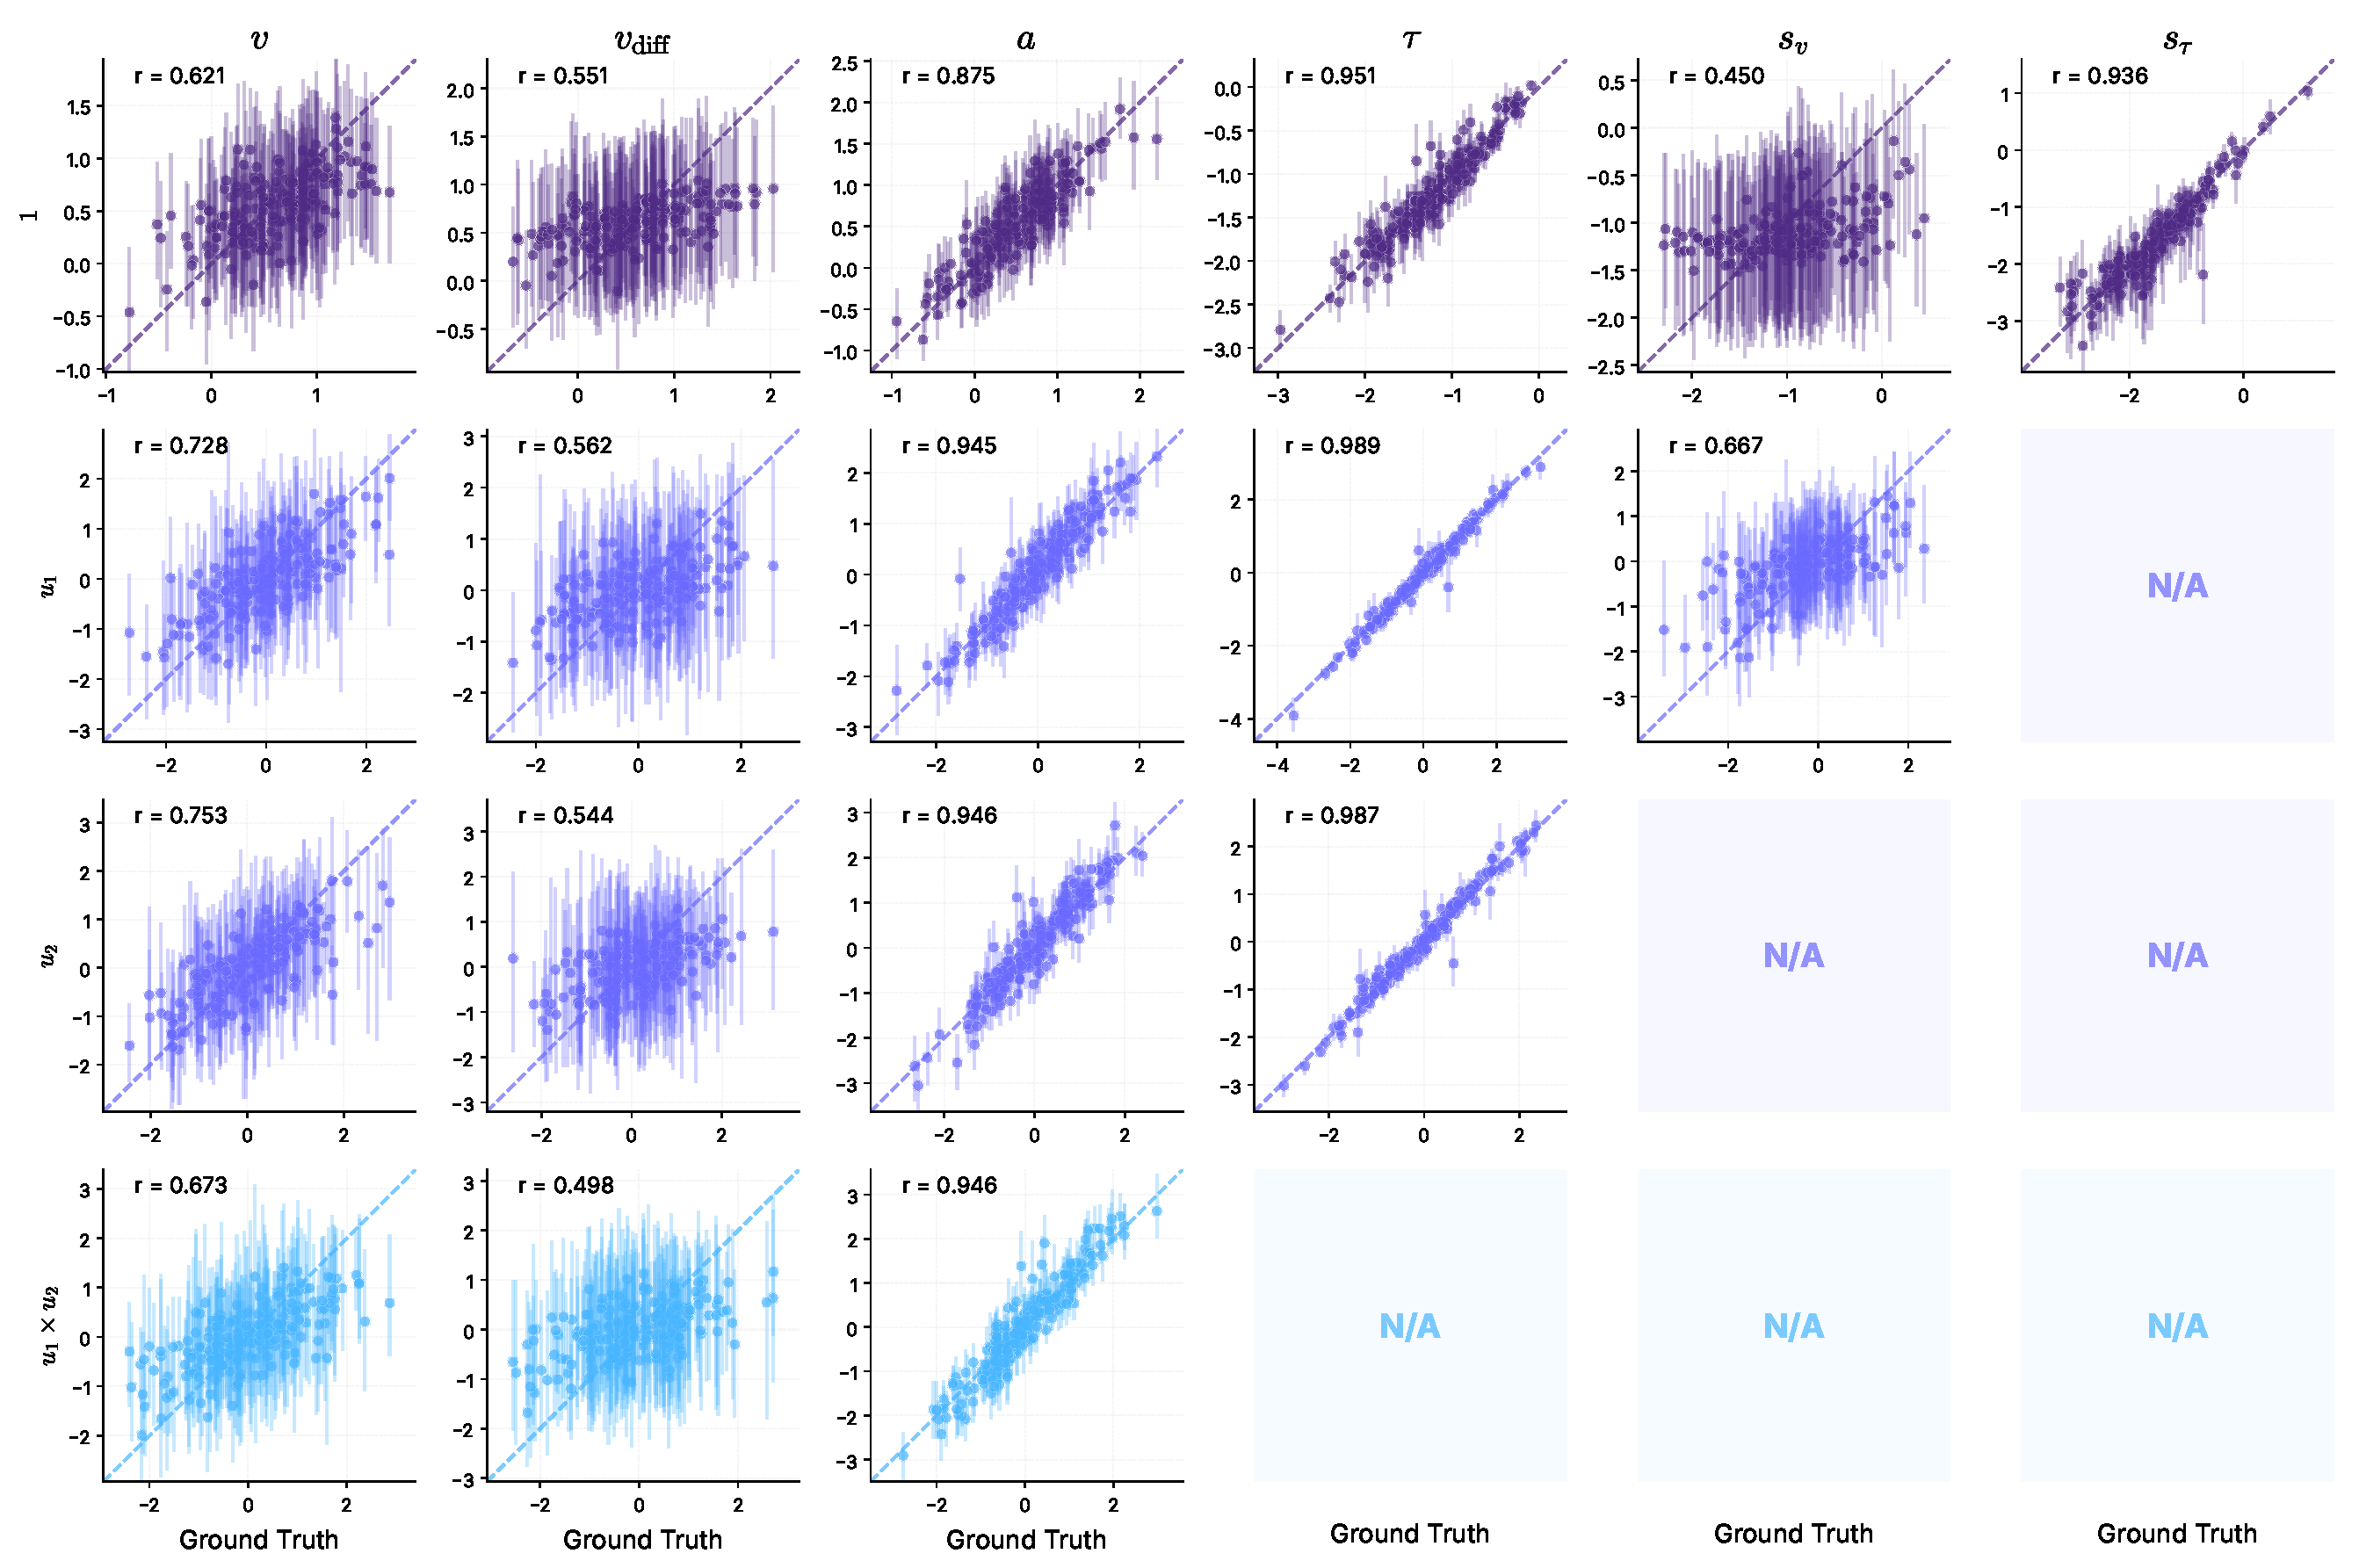
\includegraphics[width=\textwidth,height=0.3\textheight,keepaspectratio]{finetuned/rdm/interaction/recovery.pdf}
    \caption{Recovery}
  \end{subfigure}\\[1ex]
  \begin{subfigure}{\textwidth}\centering
    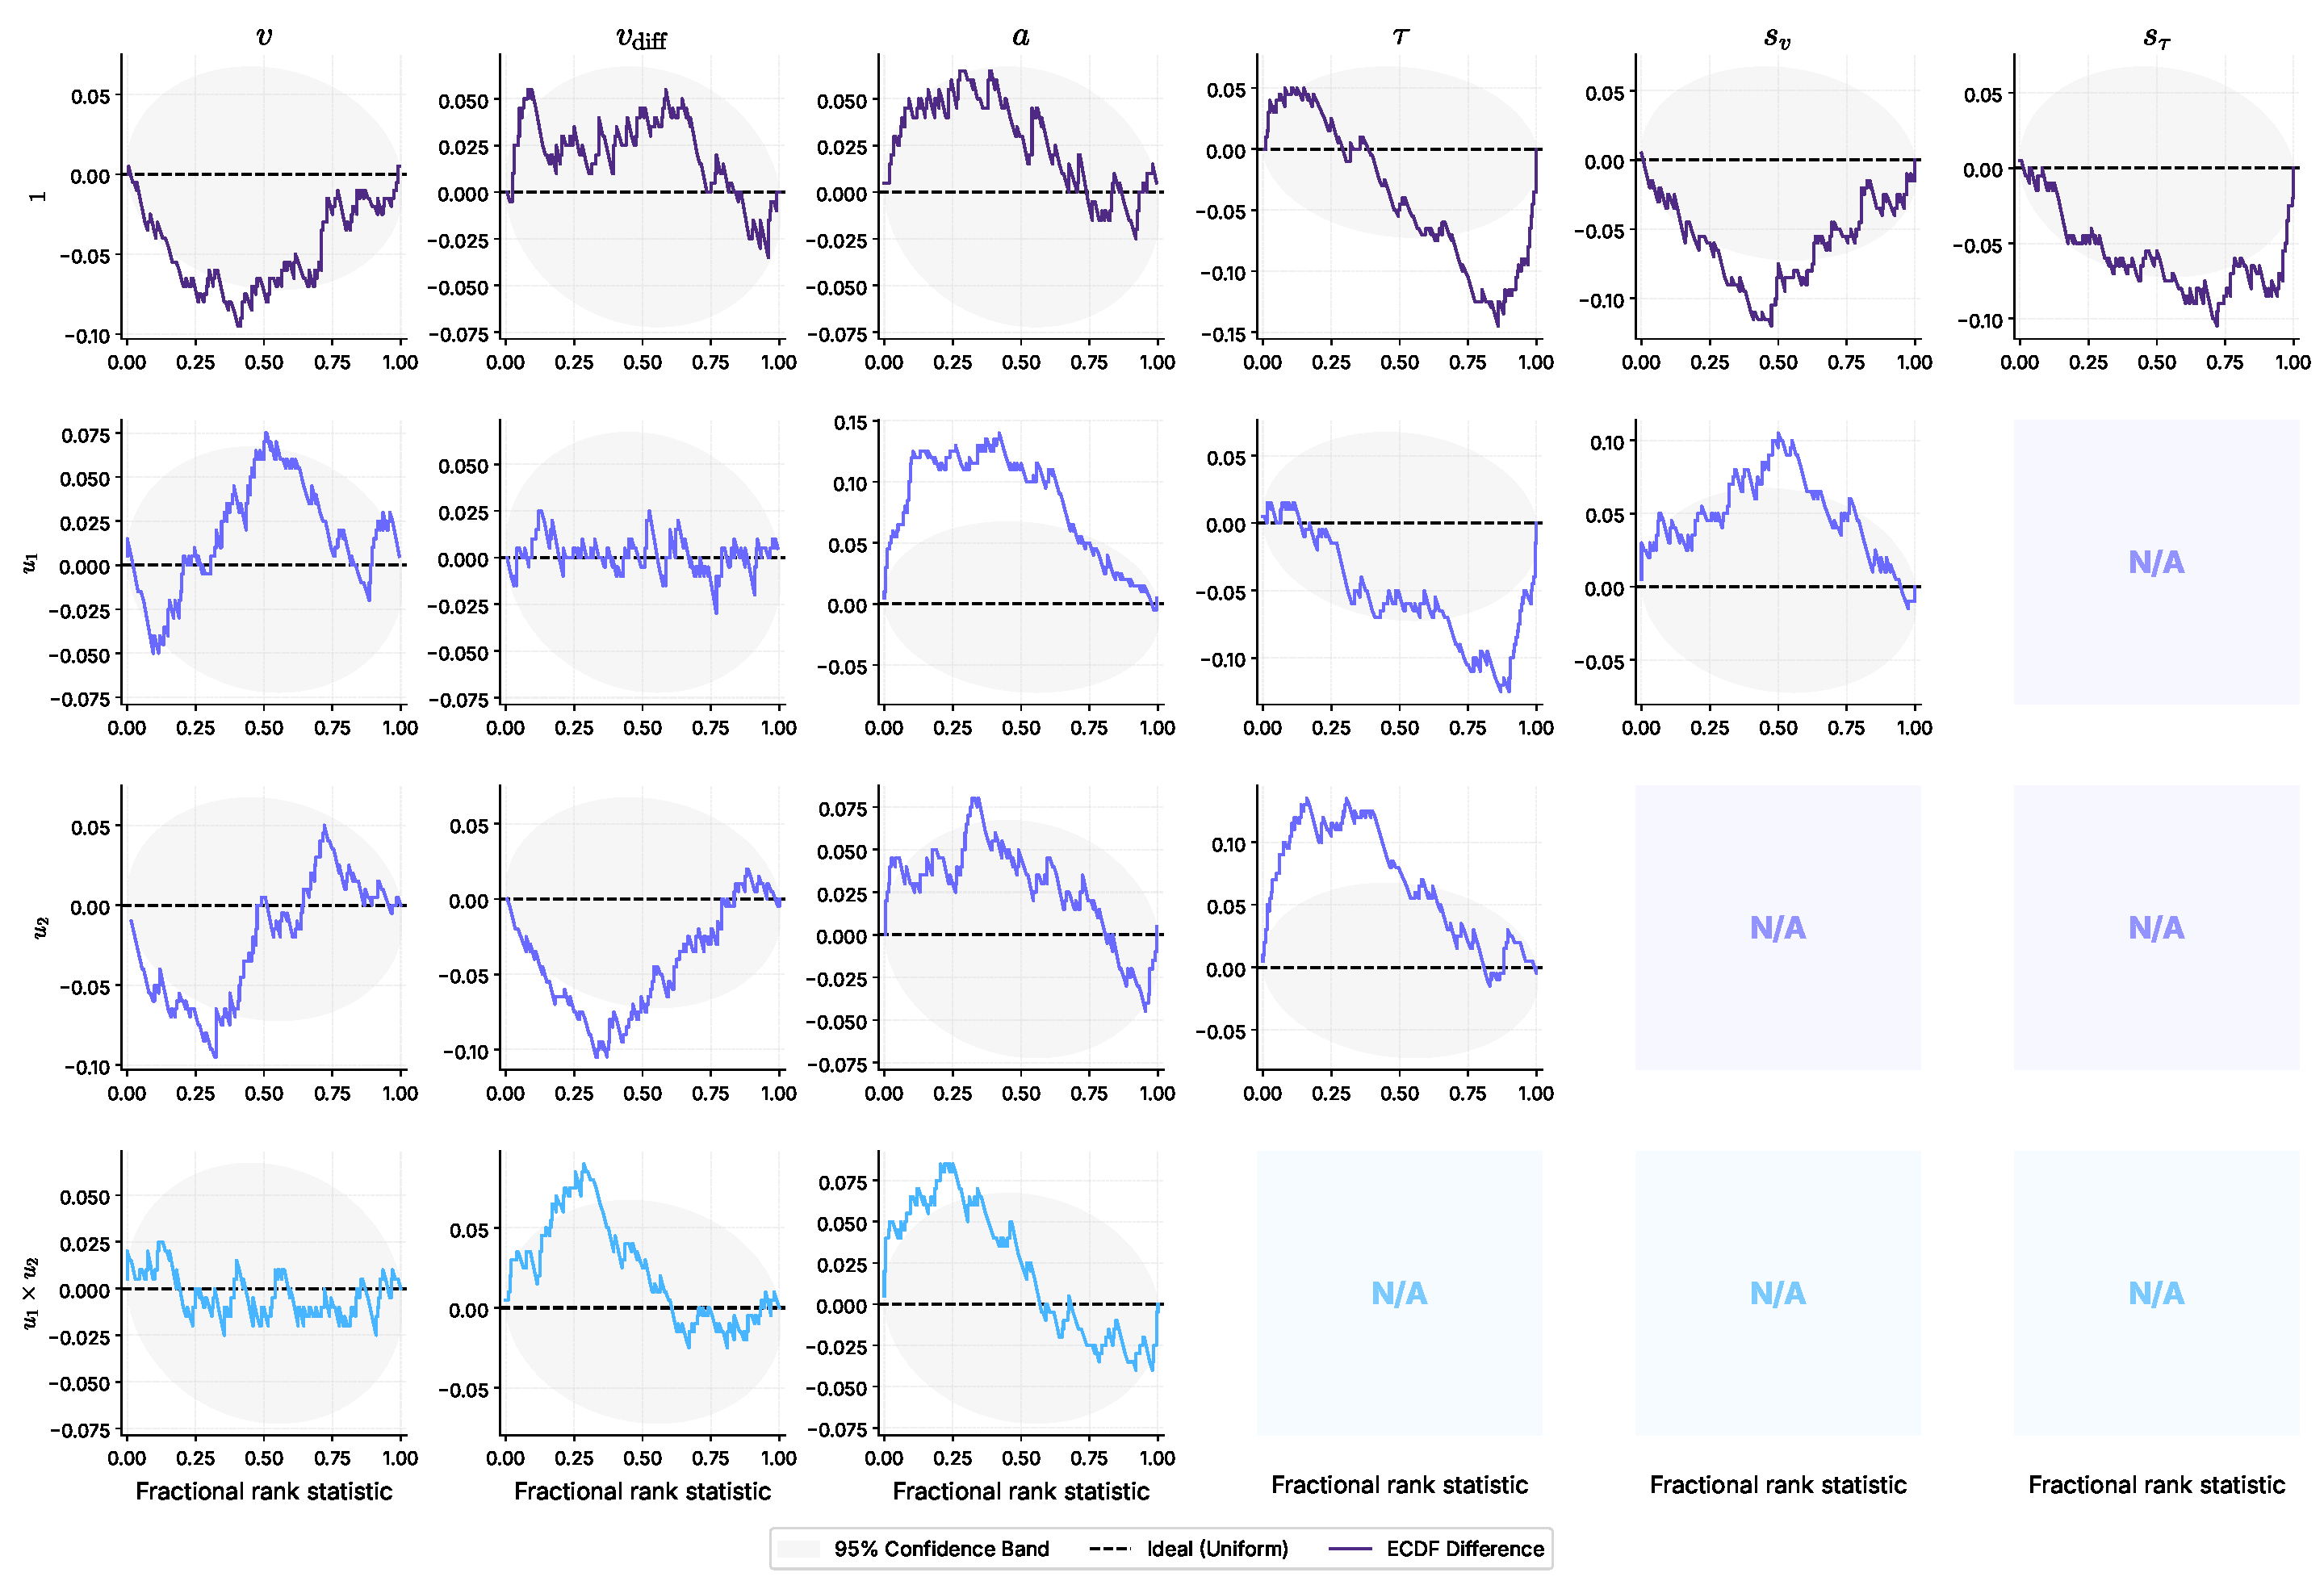
\includegraphics[width=\textwidth,height=0.3\textheight,keepaspectratio]{finetuned/rdm/interaction/ecdf.pdf}
    \caption{Calibration (ECDF)}
  \end{subfigure}\\[1ex]
  \begin{subfigure}{\textwidth}\centering
    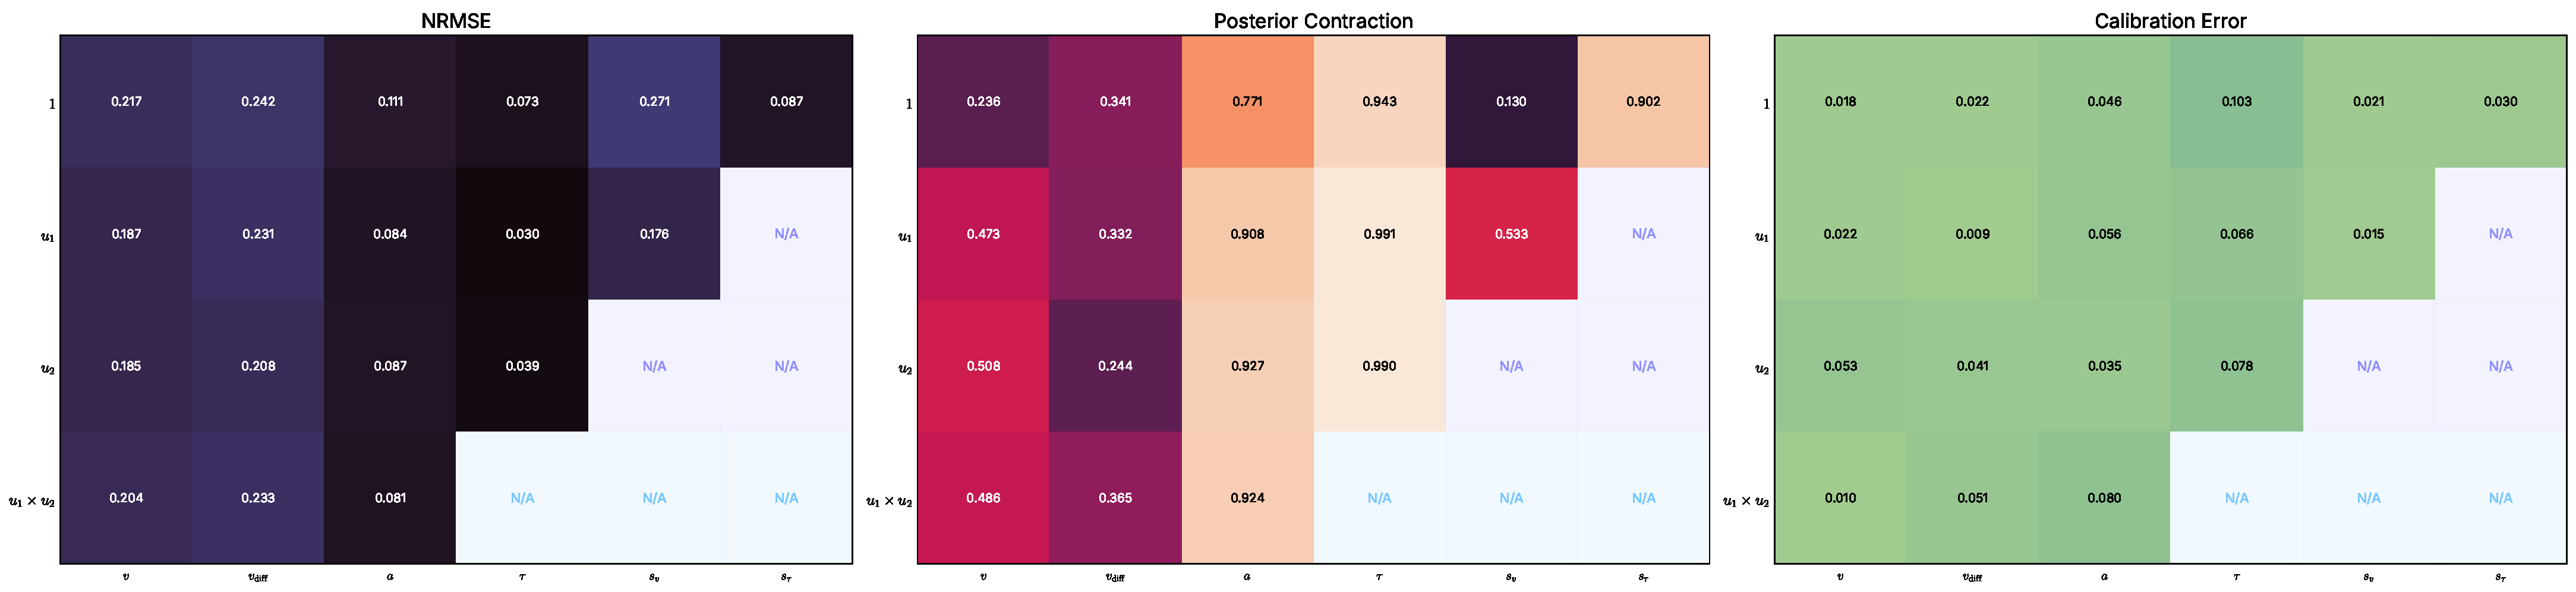
\includegraphics[width=\textwidth]{finetuned/rdm/interaction/metrics.pdf}
    \caption{Metrics}
  \end{subfigure}
  \caption{\textbf{After fine-tuning: RDM, \emph{interaction} design.} (a) Recovery, (b) calibration, (c) metrics. $v$, $v_{\mathrm{diff}}$, $a$, $\tau$ and $s_v$ carry slopes on $u_1$; $v$, $v_{\mathrm{diff}}$, $a$ and $\tau$ carry slopes on $u_2$; $v$, $v_{\mathrm{diff}}$ and $a$ on the product $u_1 u_2$ (18 coefficients shown). As in Figure~\ref{fig:app3-finetuned-lba-intercept-only}; before fine-tuning: Figure~\ref{fig:app1-rdm-interaction-cf}.}
  \label{fig:app3-finetuned-rdm-interaction}
\end{figure}

\begin{figure}[p]
  \centering
  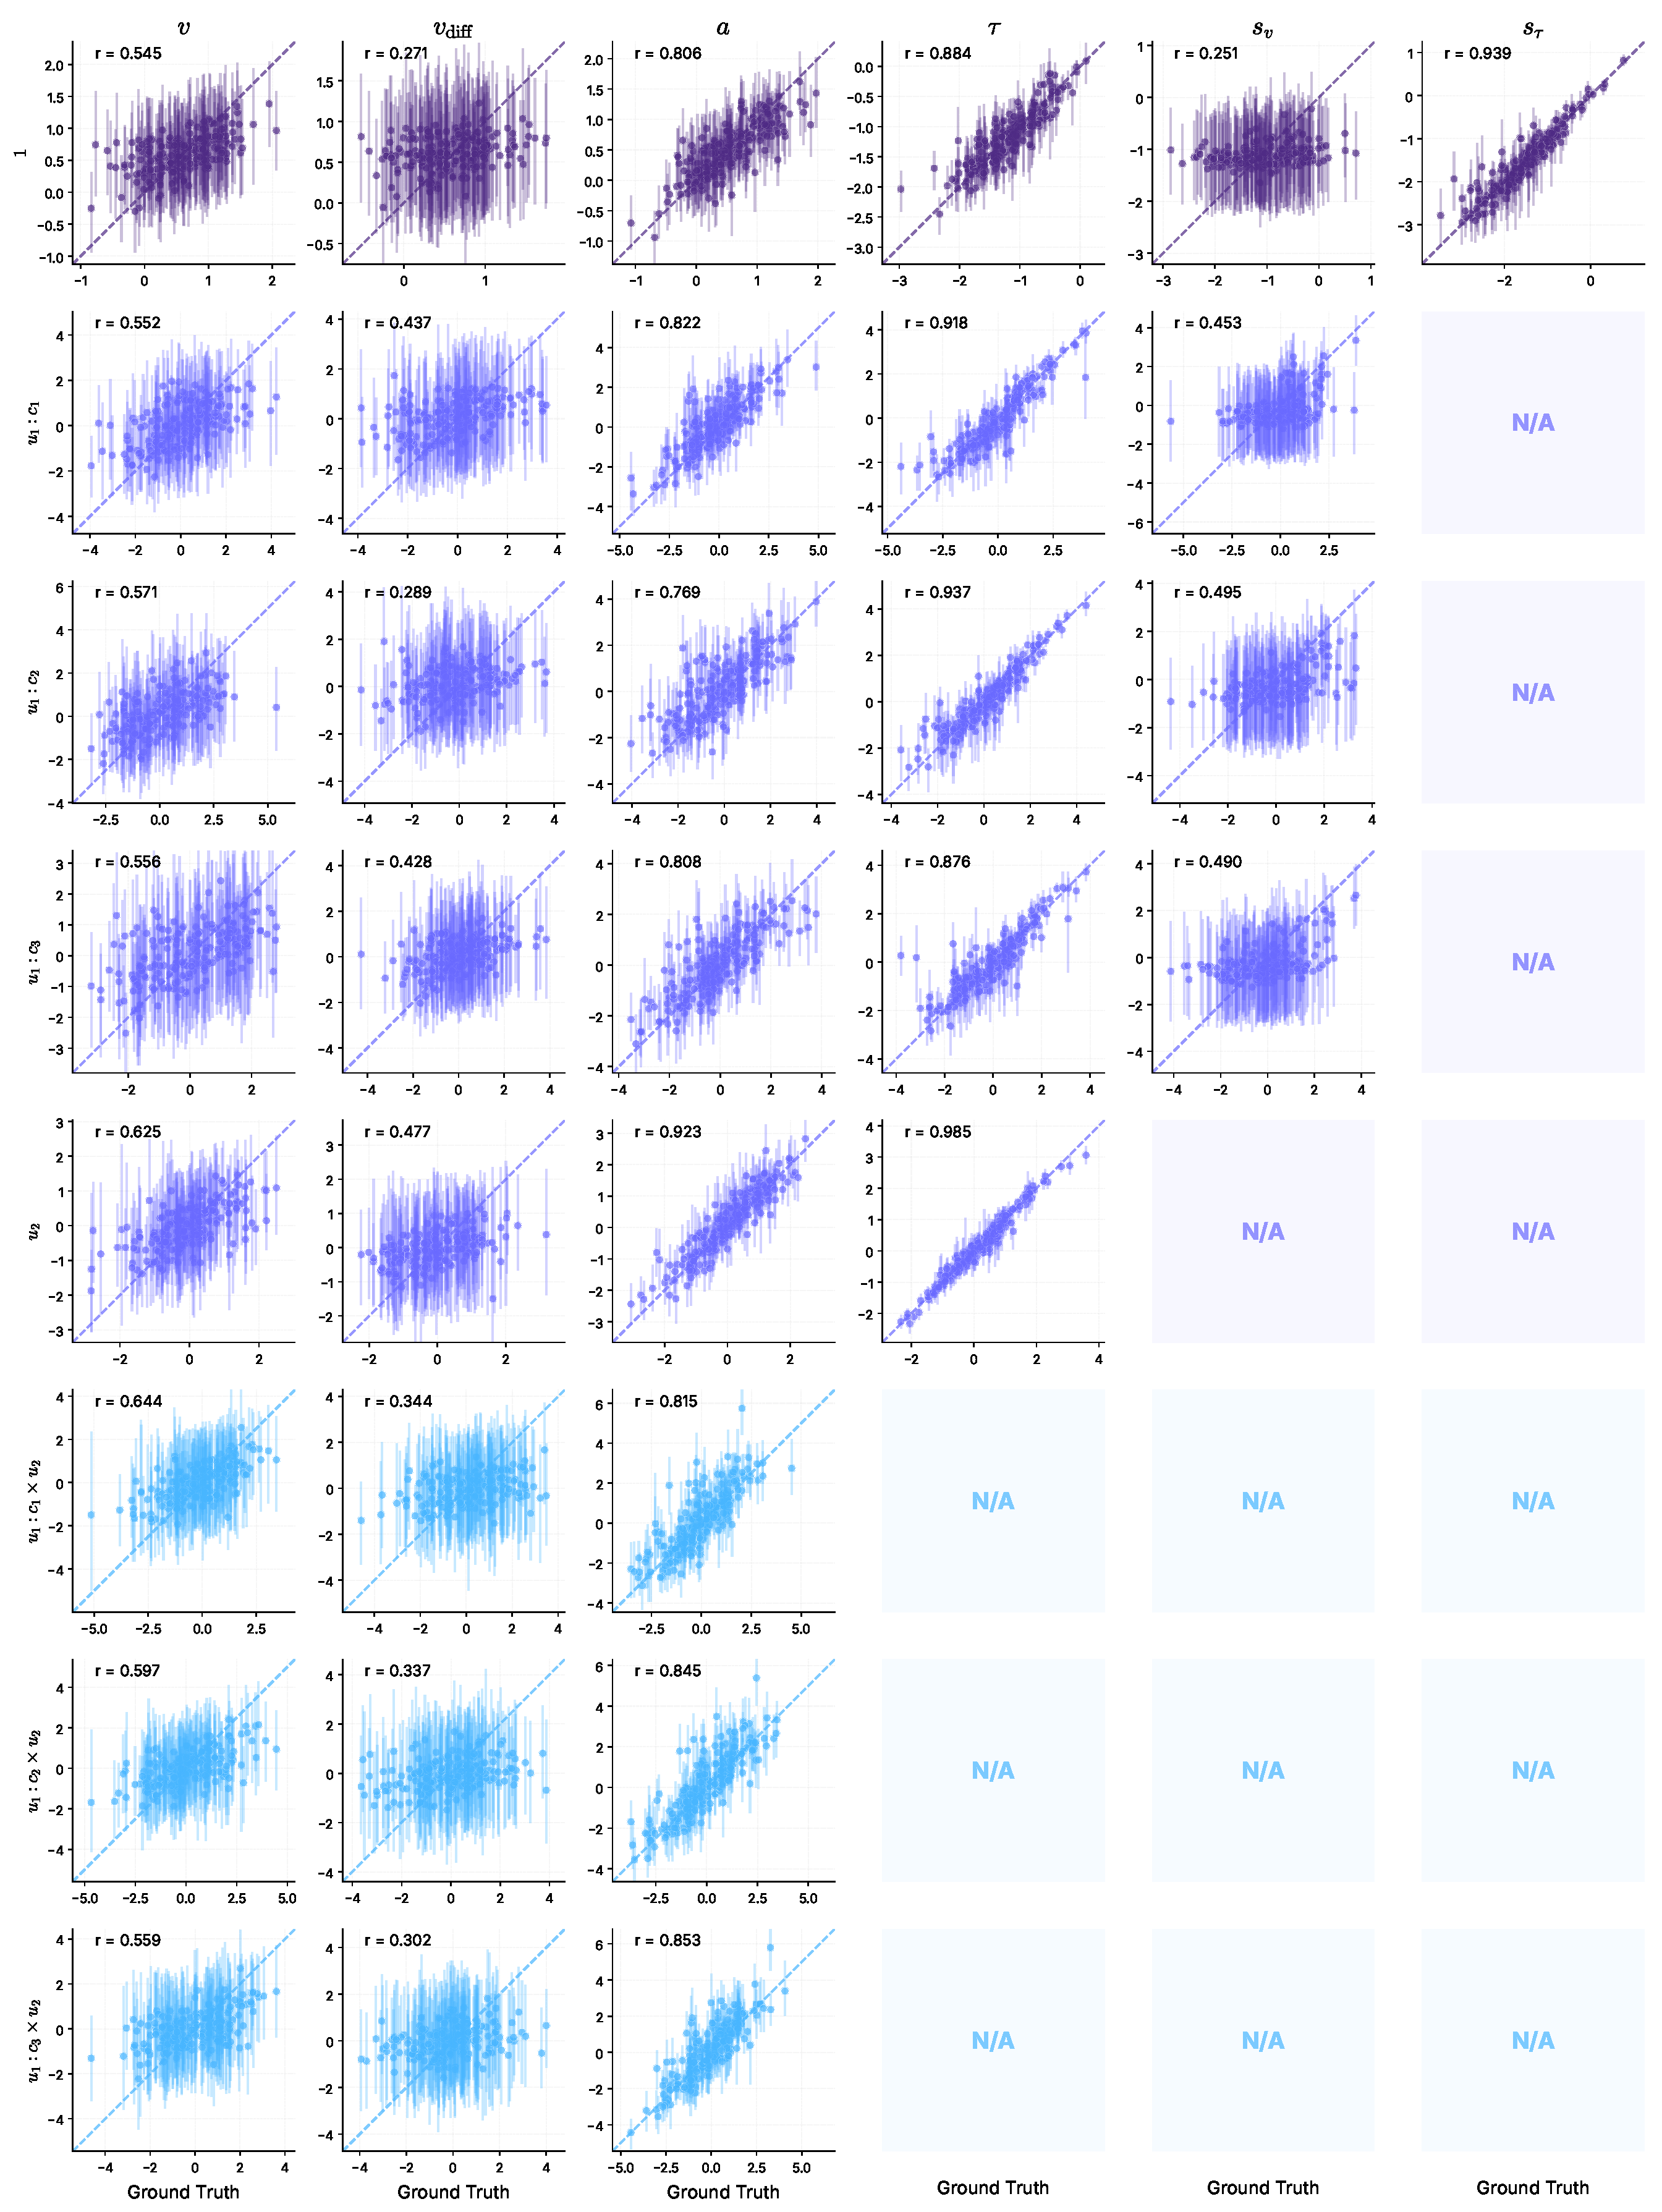
\includegraphics[width=\textwidth,height=0.82\textheight,keepaspectratio]{finetuned/rdm/mixed_predictor/recovery.pdf}
  \caption{\textbf{Parameter recovery, RDM after fine-tuning, mixed-predictor design.} $v$, $v_{\mathrm{diff}}$, $a$, $\tau$ and $s_v$ carry effects of the four-level $u_1$; $v$, $v_{\mathrm{diff}}$, $a$ and $\tau$ slopes on $u_2$; $v$, $v_{\mathrm{diff}}$ and $a$ the interaction (34 coefficients shown). Datasets simulated for this design (no shared benchmark file exists); design as in Figure~\ref{fig:app1-ddm-mixed-predictor-recovery}, encoding as in the top panel of Figure~\ref{fig:app1-ddm-intercept-only-cf}.}
  \label{fig:app3-finetuned-rdm-mixed-predictor-recovery}
\end{figure}

\begin{figure}[p]
  \centering
  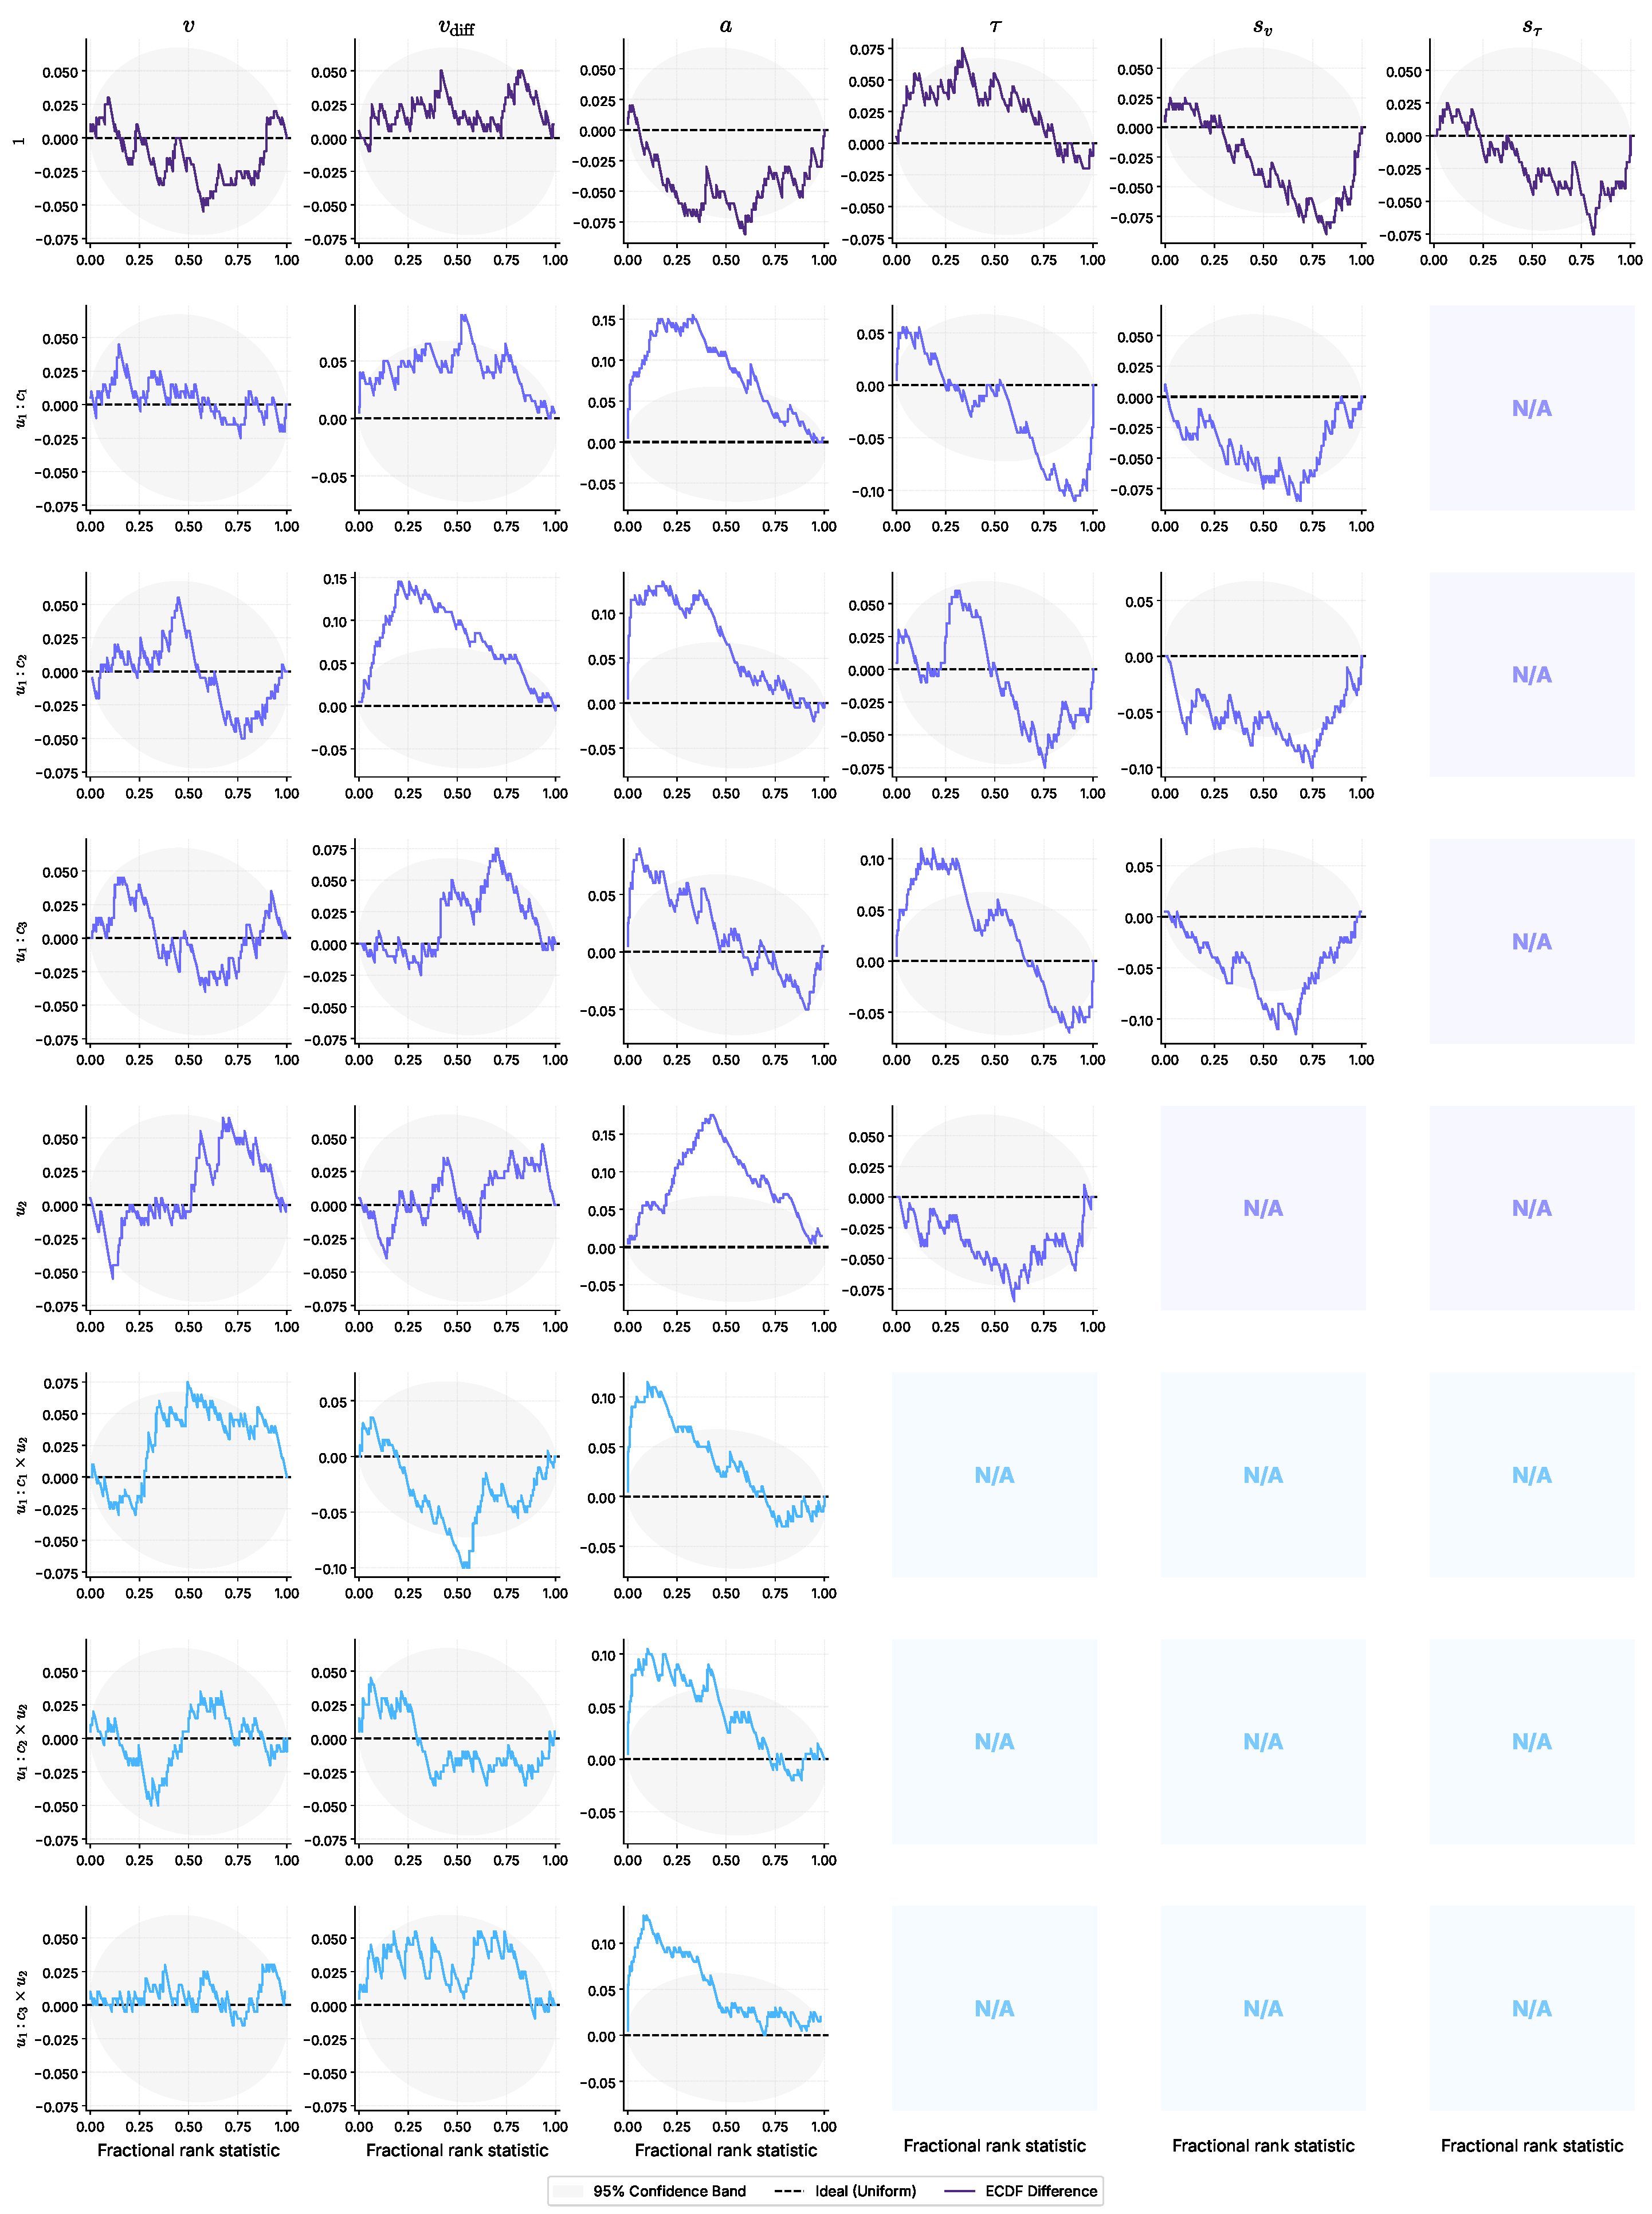
\includegraphics[width=\textwidth,height=0.82\textheight,keepaspectratio]{finetuned/rdm/mixed_predictor/ecdf.pdf}
  \caption{\textbf{Simulation-based calibration, RDM after fine-tuning, mixed-predictor design.} $v$, $v_{\mathrm{diff}}$, $a$, $\tau$ and $s_v$ carry effects of the four-level $u_1$; $v$, $v_{\mathrm{diff}}$, $a$ and $\tau$ slopes on $u_2$; $v$, $v_{\mathrm{diff}}$ and $a$ the interaction (34 coefficients shown). Datasets simulated for this design (no shared benchmark file exists); design as in Figure~\ref{fig:app1-ddm-mixed-predictor-recovery}, encoding as in the middle panel of Figure~\ref{fig:app1-ddm-intercept-only-cf}.}
  \label{fig:app3-finetuned-rdm-mixed-predictor-ecdf}
\end{figure}

\begin{figure}[p]
  \centering
  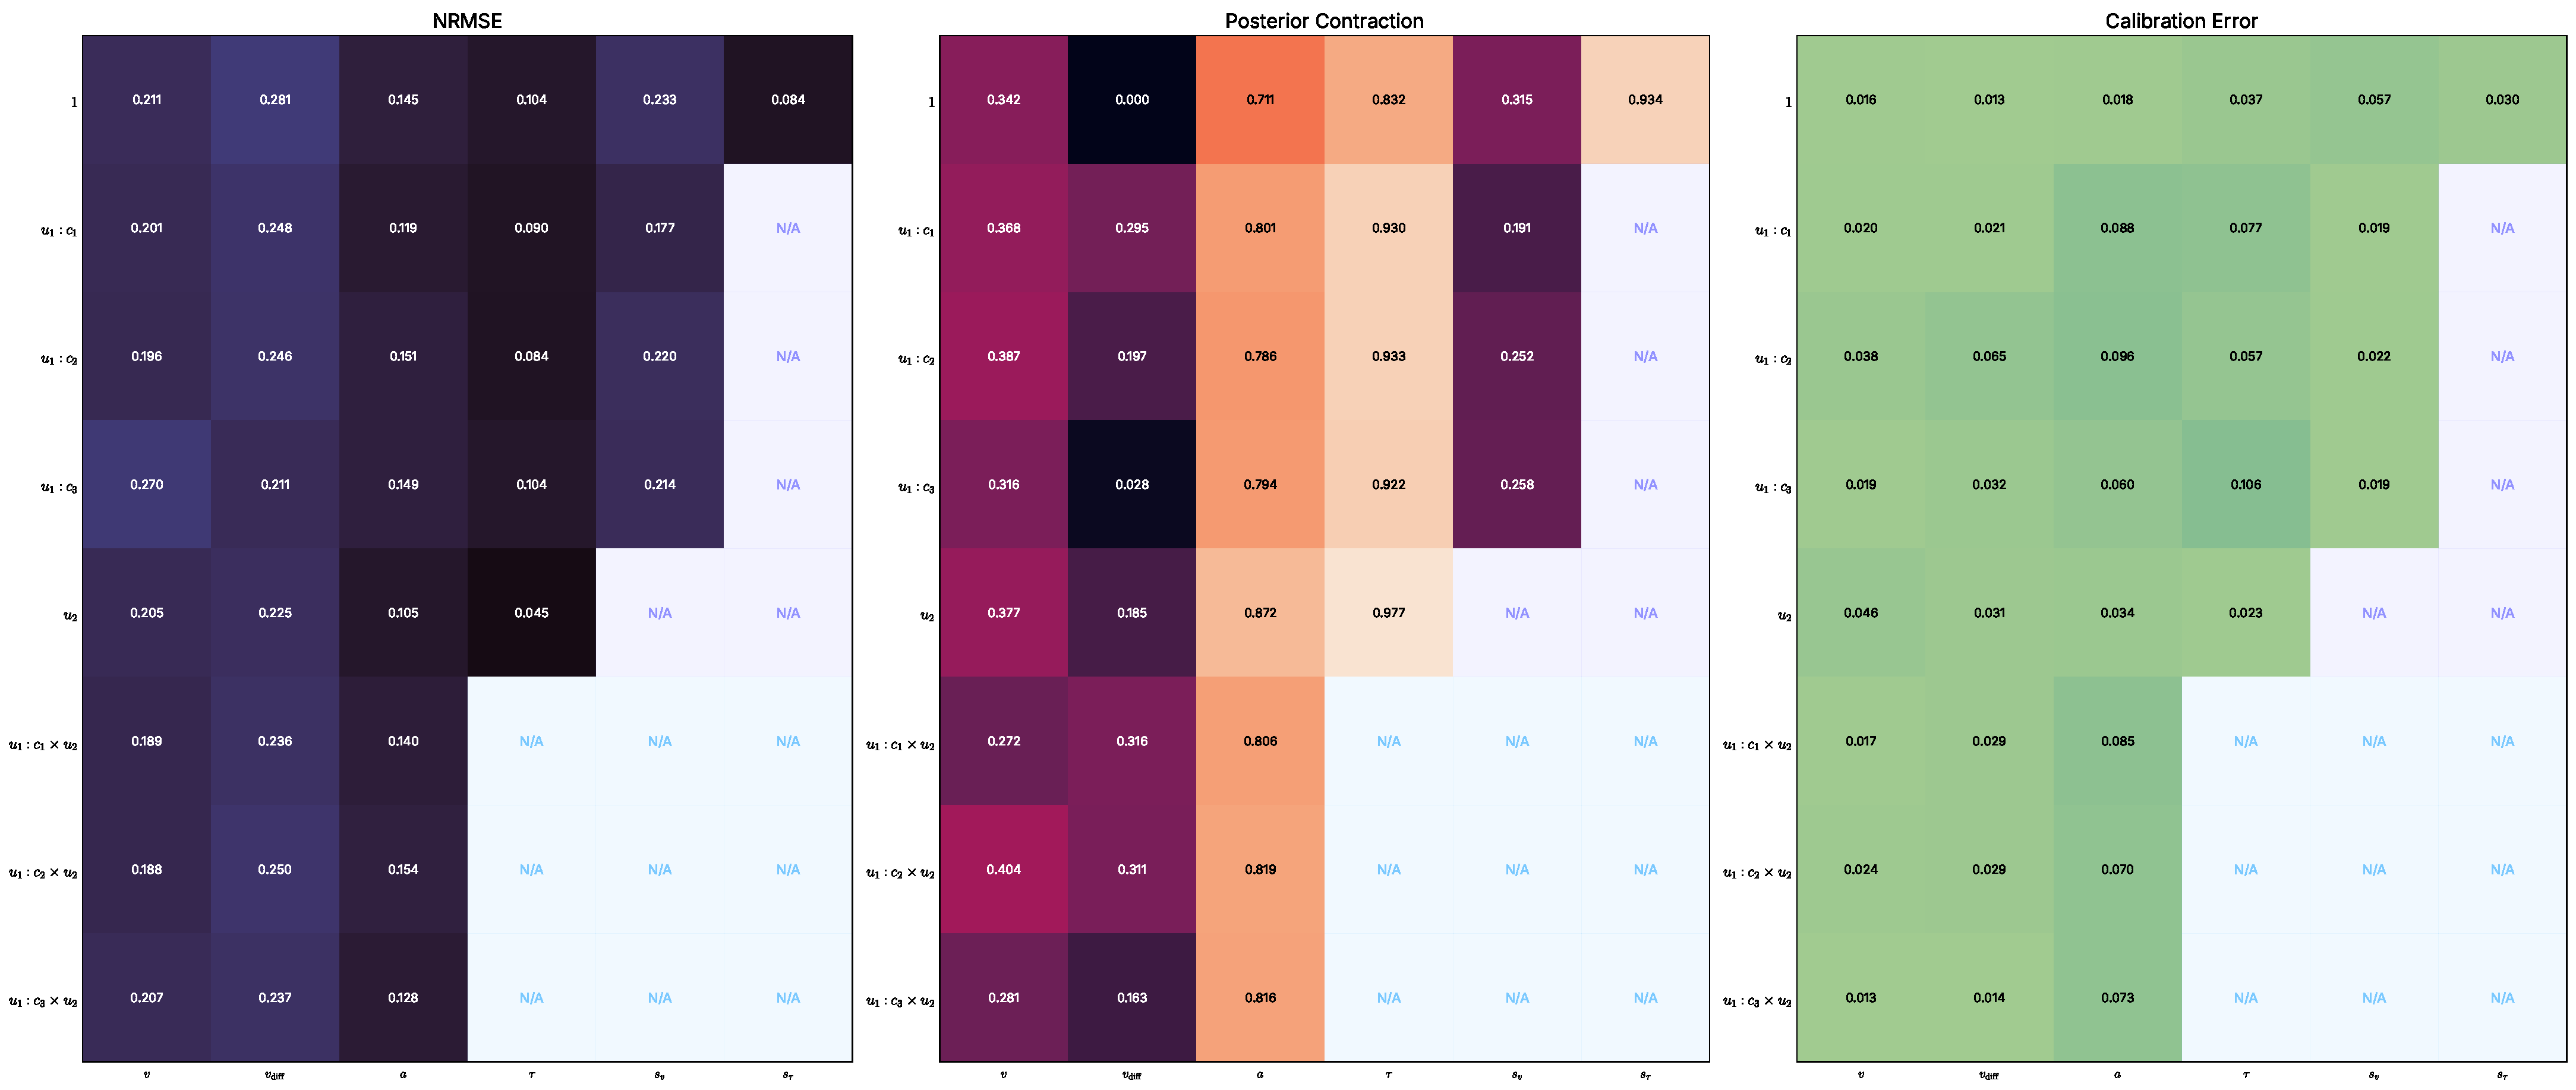
\includegraphics[width=\textwidth,height=0.82\textheight,keepaspectratio]{finetuned/rdm/mixed_predictor/metrics.pdf}
  \caption{\textbf{Summary metrics, RDM after fine-tuning, mixed-predictor design.} $v$, $v_{\mathrm{diff}}$, $a$, $\tau$ and $s_v$ carry effects of the four-level $u_1$; $v$, $v_{\mathrm{diff}}$, $a$ and $\tau$ slopes on $u_2$; $v$, $v_{\mathrm{diff}}$ and $a$ the interaction (34 coefficients shown). Datasets simulated for this design (no shared benchmark file exists); design as in Figure~\ref{fig:app1-ddm-mixed-predictor-recovery}, encoding as in the bottom panel of Figure~\ref{fig:app1-ddm-intercept-only-cf}.}
  \label{fig:app3-finetuned-rdm-mixed-predictor-metrics}
\end{figure}

\begin{figure}[p]
  \centering
  \begin{subfigure}{\textwidth}\centering
    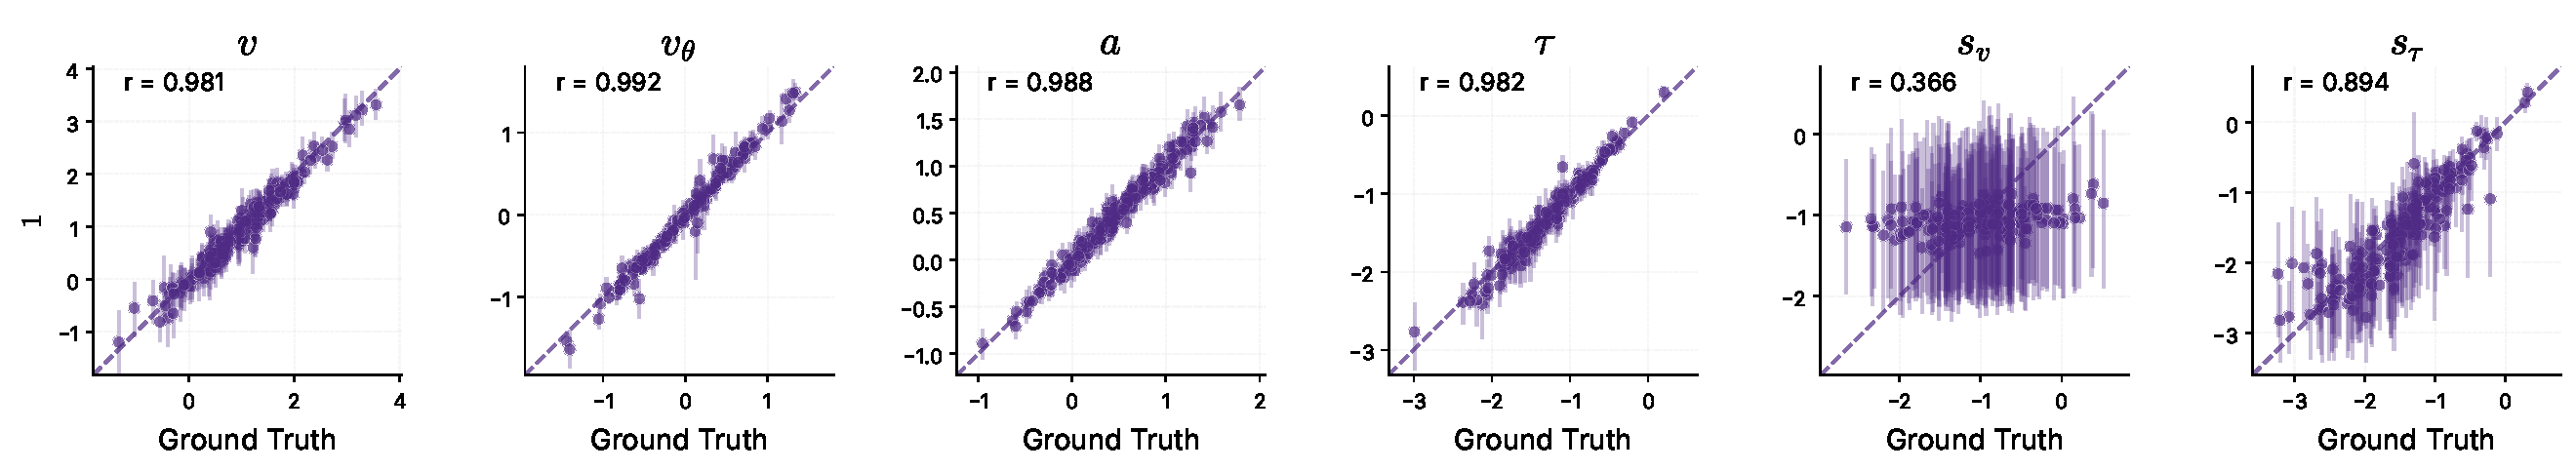
\includegraphics[width=\textwidth,height=0.3\textheight,keepaspectratio]{finetuned/cdm/intercept_only/recovery.pdf}
    \caption{Recovery}
  \end{subfigure}\\[1ex]
  \begin{subfigure}{\textwidth}\centering
    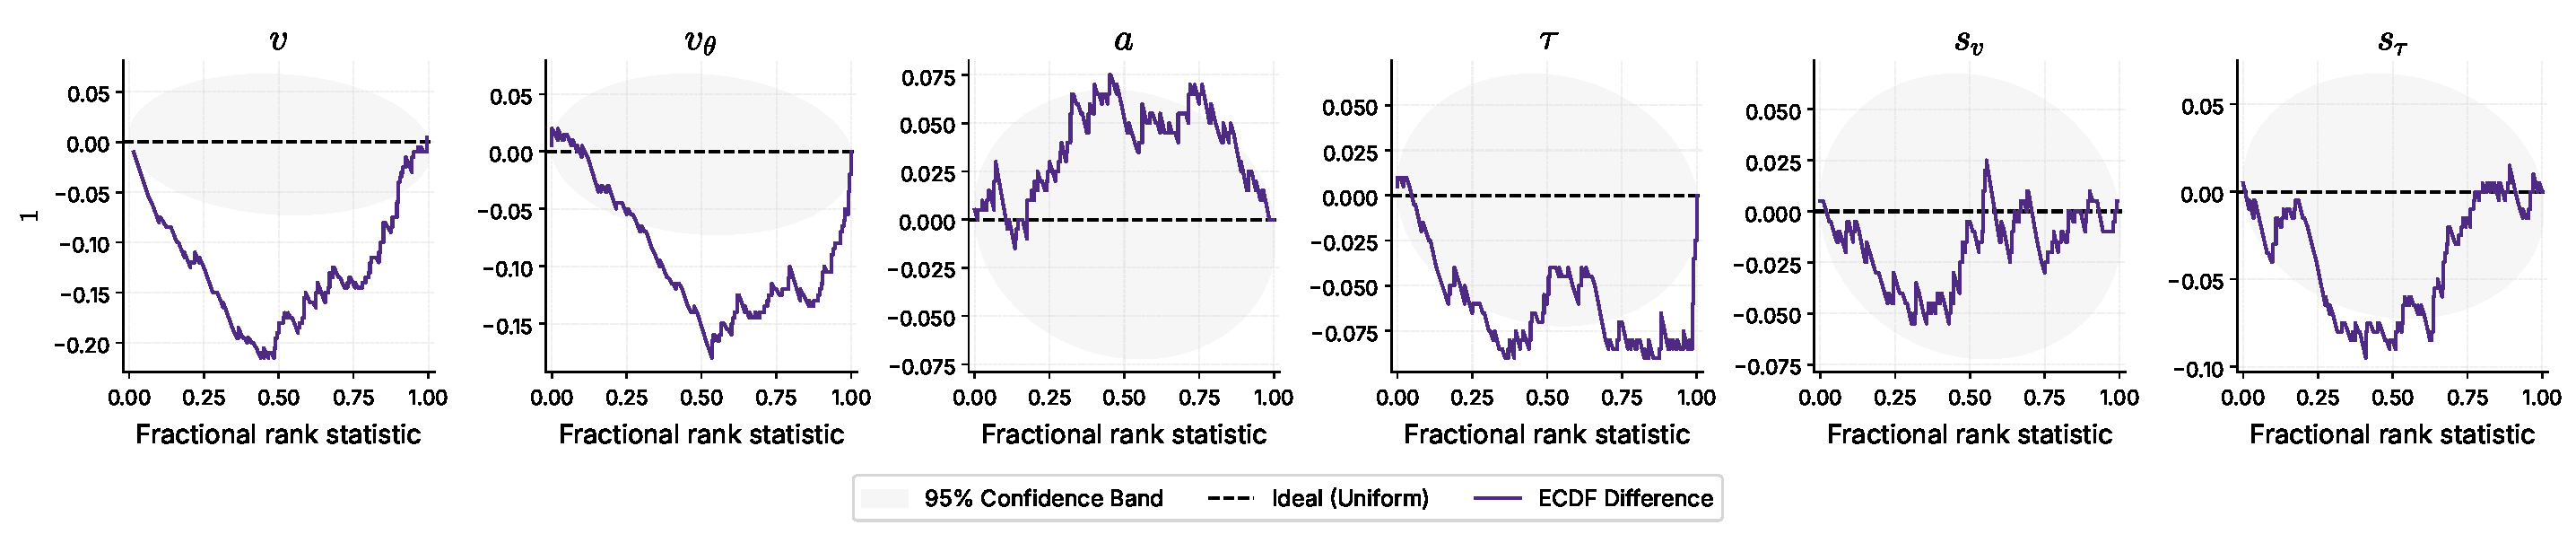
\includegraphics[width=\textwidth,height=0.3\textheight,keepaspectratio]{finetuned/cdm/intercept_only/ecdf.pdf}
    \caption{Calibration (ECDF)}
  \end{subfigure}\\[1ex]
  \begin{subfigure}{\textwidth}\centering
    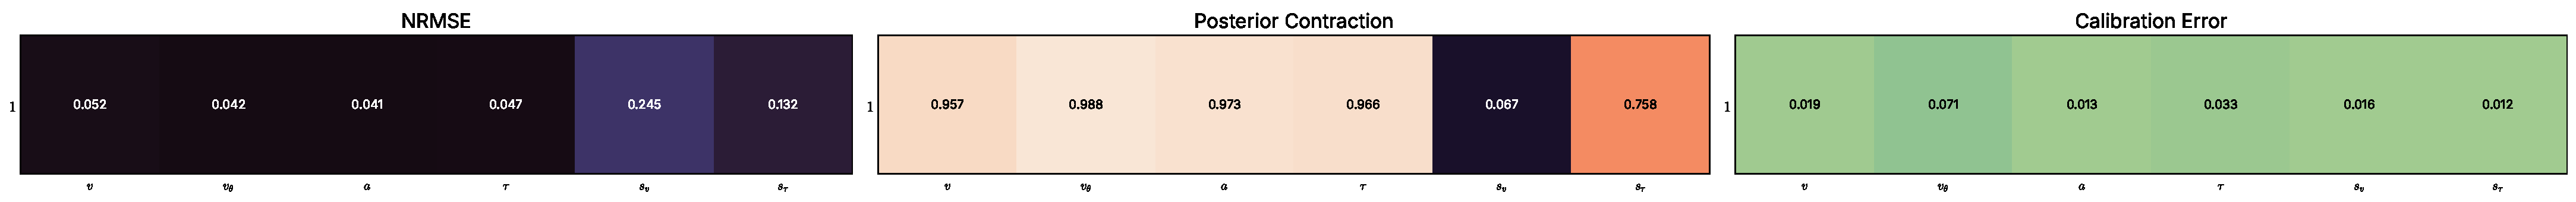
\includegraphics[width=\textwidth]{finetuned/cdm/intercept_only/metrics.pdf}
    \caption{Metrics}
  \end{subfigure}
  \caption{\textbf{After fine-tuning: CDM, \emph{intercept-only} design.} (a) Recovery, (b) calibration, (c) metrics. Every estimated parameter enters as an intercept only (6 coefficients shown). As in Figure~\ref{fig:app3-finetuned-lba-intercept-only}; before fine-tuning: Figure~\ref{fig:app1-cdm-intercept-only-cf}.}
  \label{fig:app3-finetuned-cdm-intercept-only}
\end{figure}

\begin{figure}[p]
  \centering
  \begin{subfigure}{\textwidth}\centering
    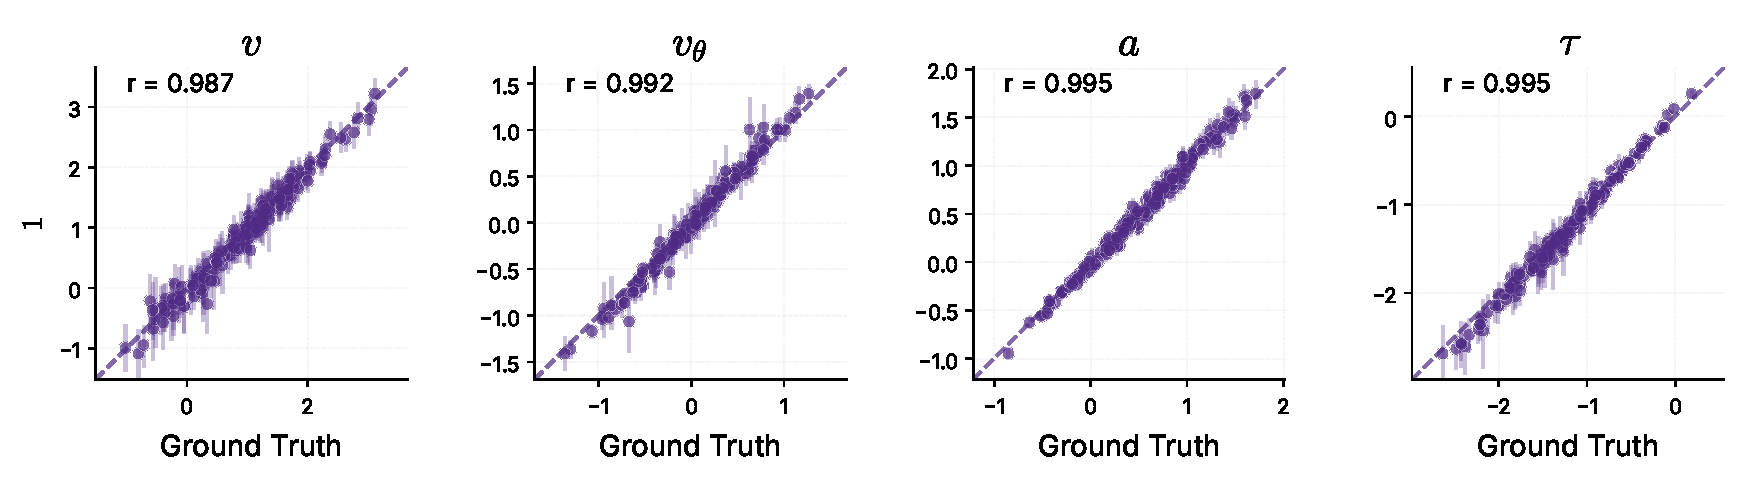
\includegraphics[width=\textwidth,height=0.3\textheight,keepaspectratio]{finetuned/cdm/fixed/recovery.pdf}
    \caption{Recovery}
  \end{subfigure}\\[1ex]
  \begin{subfigure}{\textwidth}\centering
    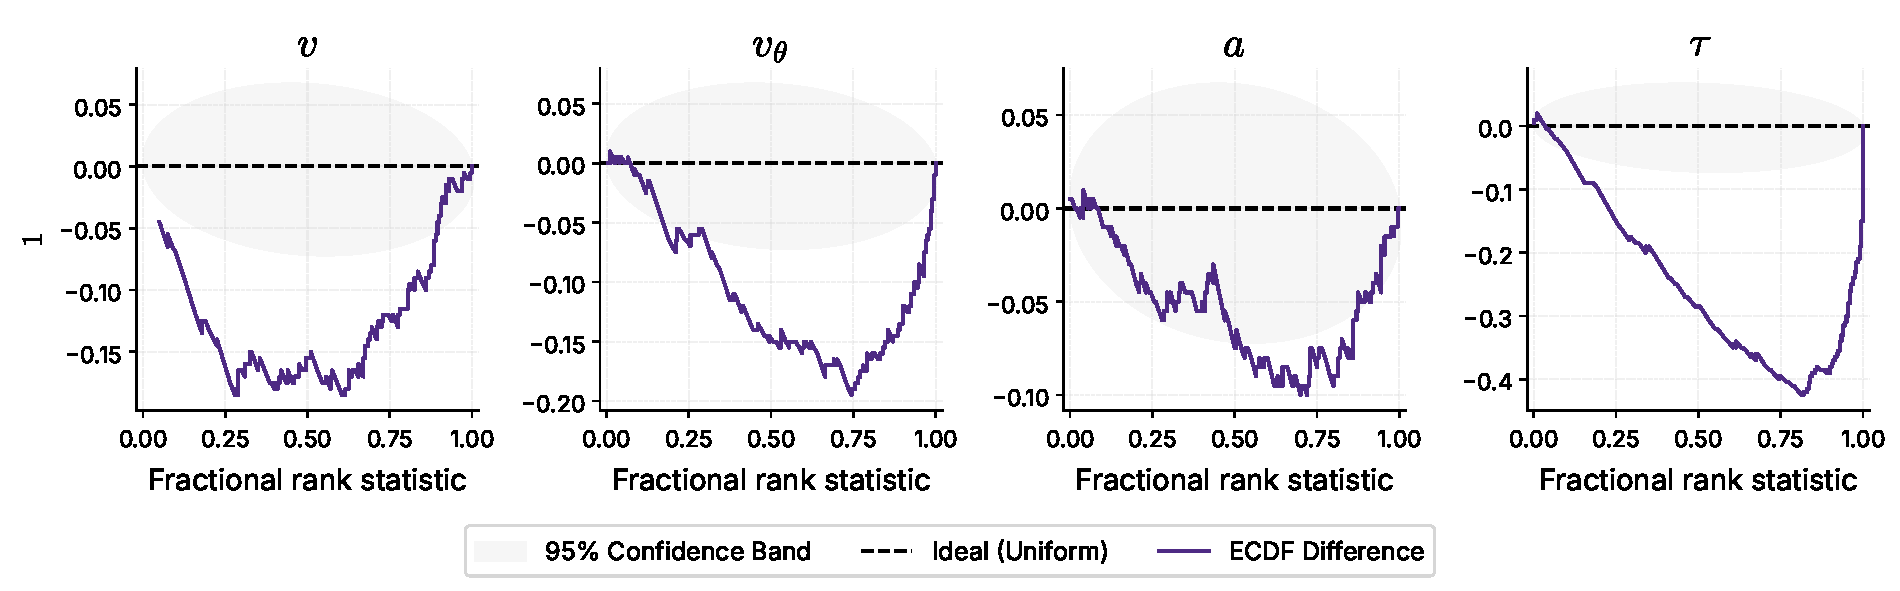
\includegraphics[width=\textwidth,height=0.3\textheight,keepaspectratio]{finetuned/cdm/fixed/ecdf.pdf}
    \caption{Calibration (ECDF)}
  \end{subfigure}\\[1ex]
  \begin{subfigure}{\textwidth}\centering
    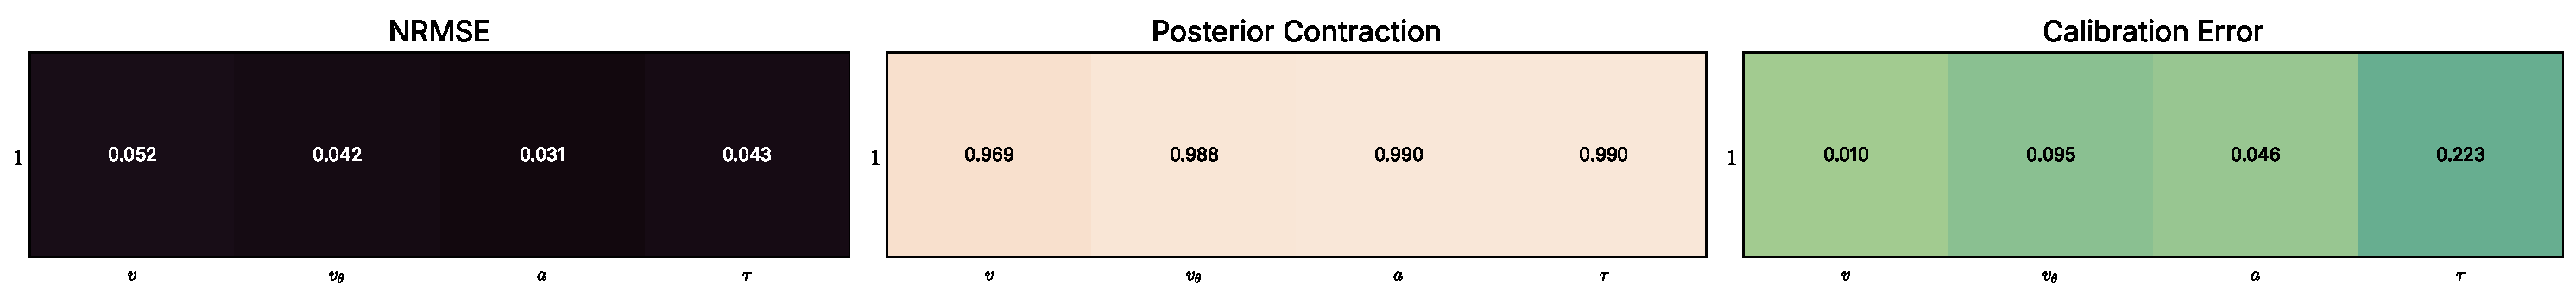
\includegraphics[width=\textwidth]{finetuned/cdm/fixed/metrics.pdf}
    \caption{Metrics}
  \end{subfigure}
  \caption{\textbf{After fine-tuning: CDM, \emph{fixed} design.} (a) Recovery, (b) calibration, (c) metrics. $s_v$ and $s_\tau$ are fixed at 0 and not estimated; every estimated parameter enters as an intercept only (4 coefficients shown). As in Figure~\ref{fig:app3-finetuned-lba-intercept-only}; before fine-tuning: Figure~\ref{fig:app1-cdm-fixed-cf}.}
  \label{fig:app3-finetuned-cdm-fixed}
\end{figure}

\begin{figure}[p]
  \centering
  \begin{subfigure}{\textwidth}\centering
    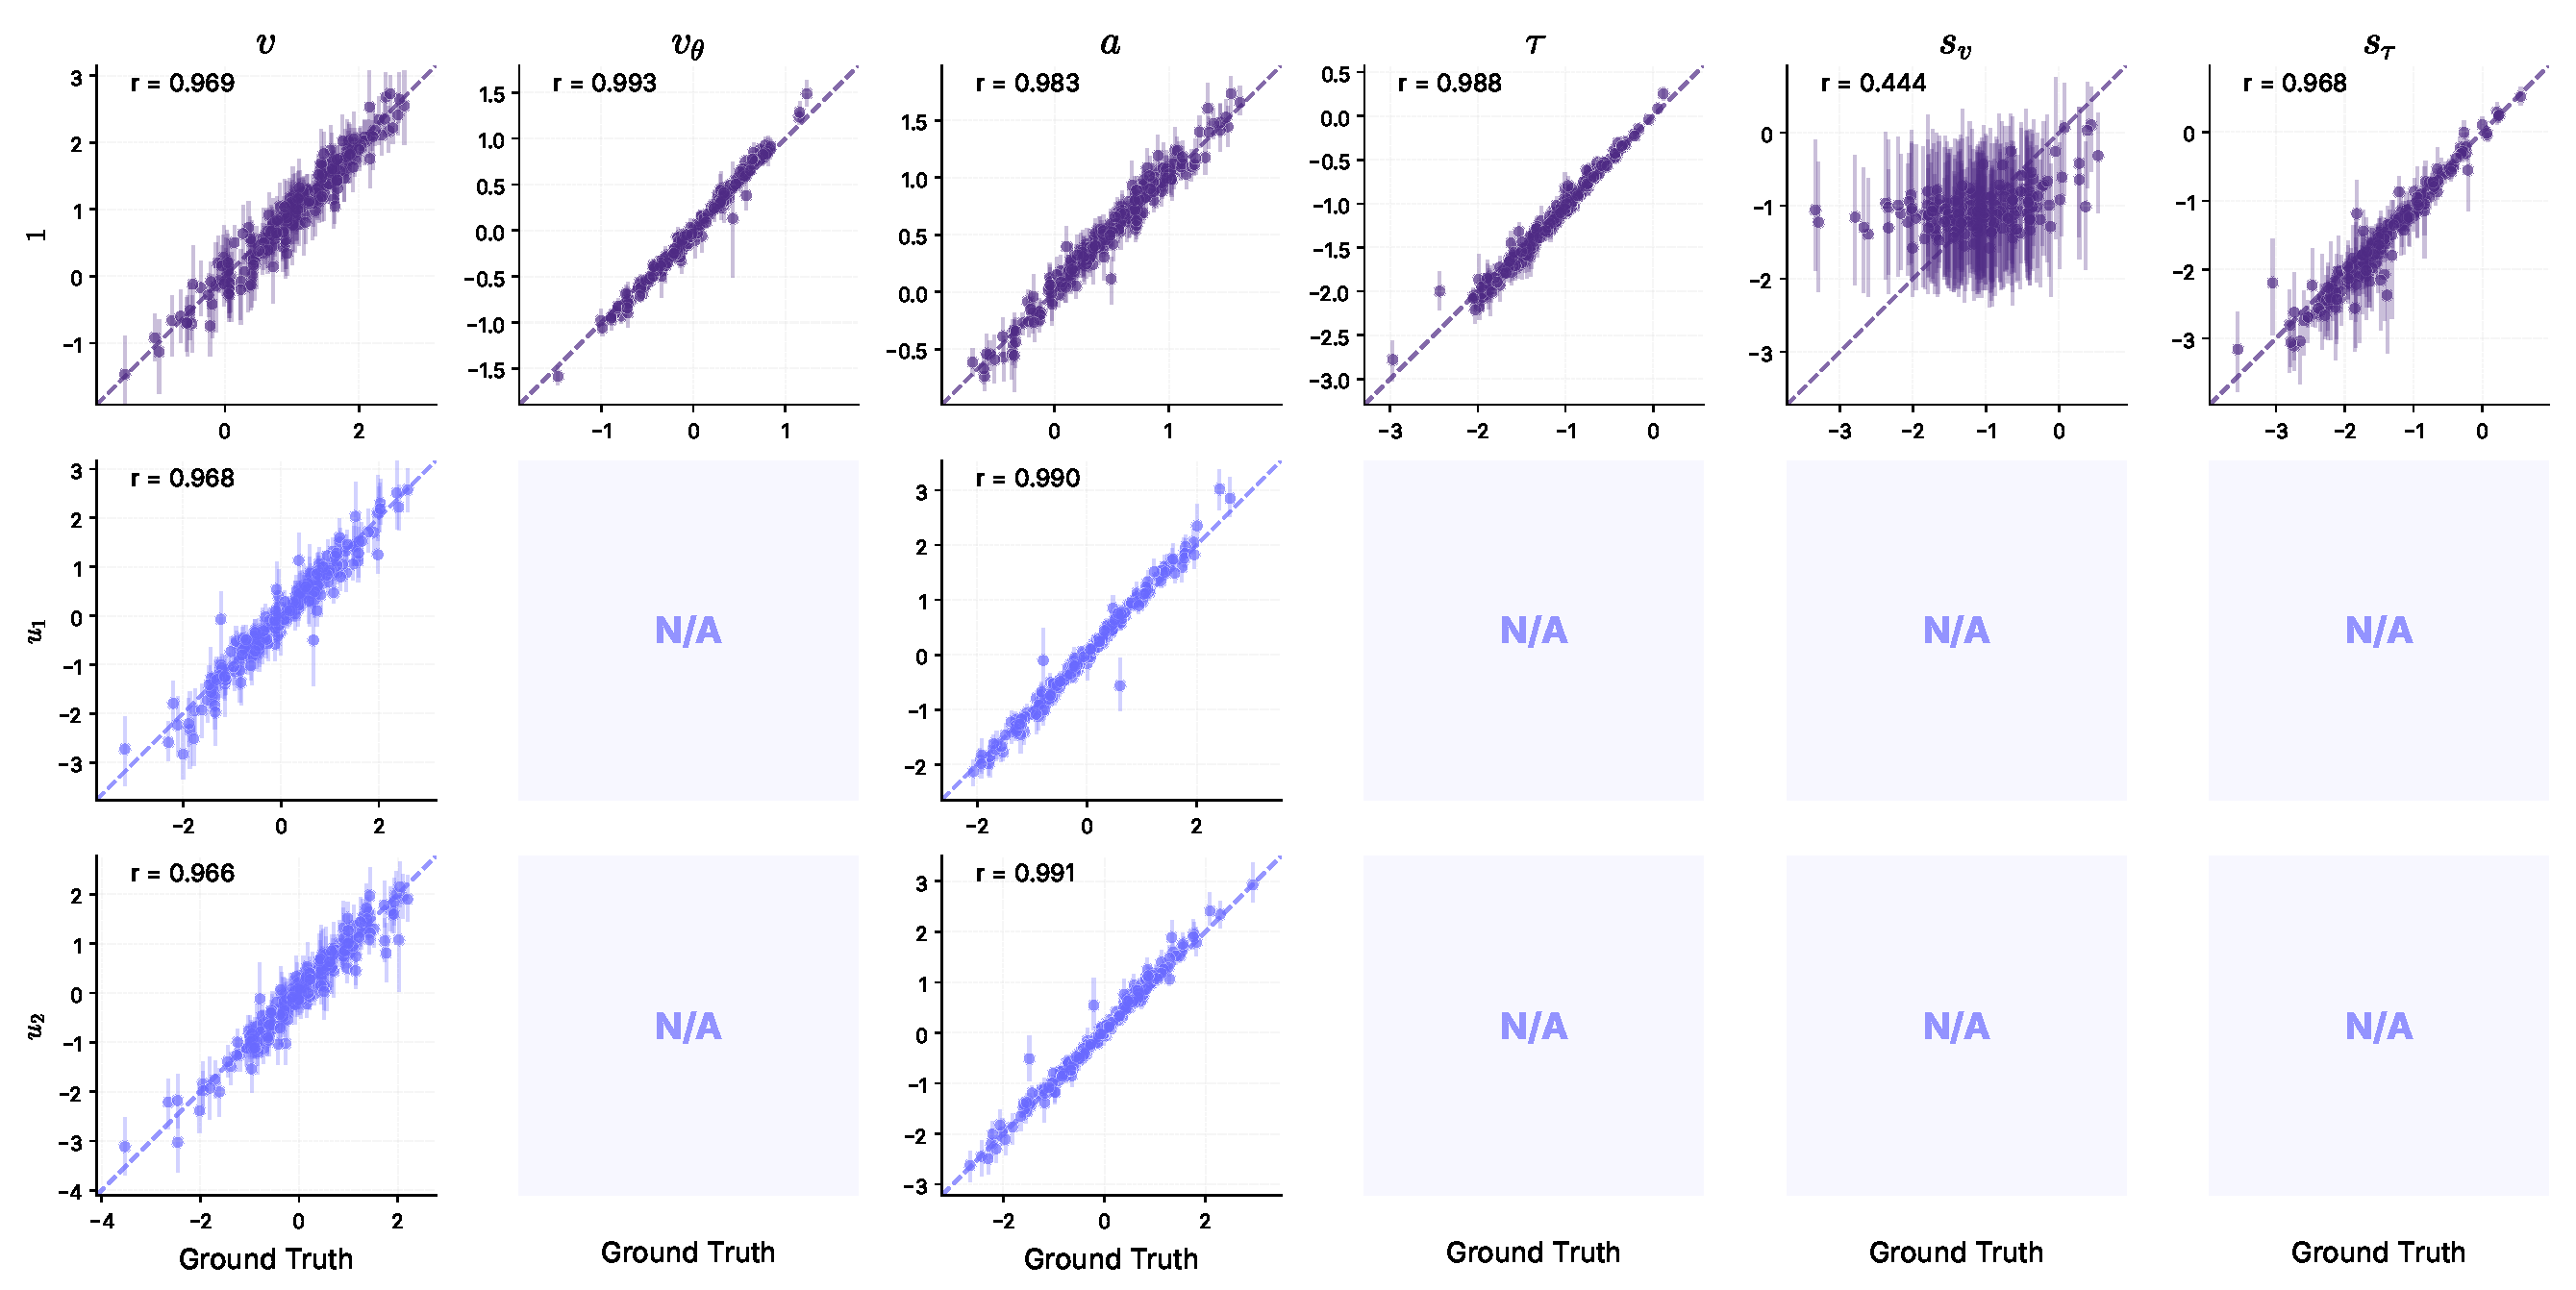
\includegraphics[width=\textwidth,height=0.3\textheight,keepaspectratio]{finetuned/cdm/regressed/recovery.pdf}
    \caption{Recovery}
  \end{subfigure}\\[1ex]
  \begin{subfigure}{\textwidth}\centering
    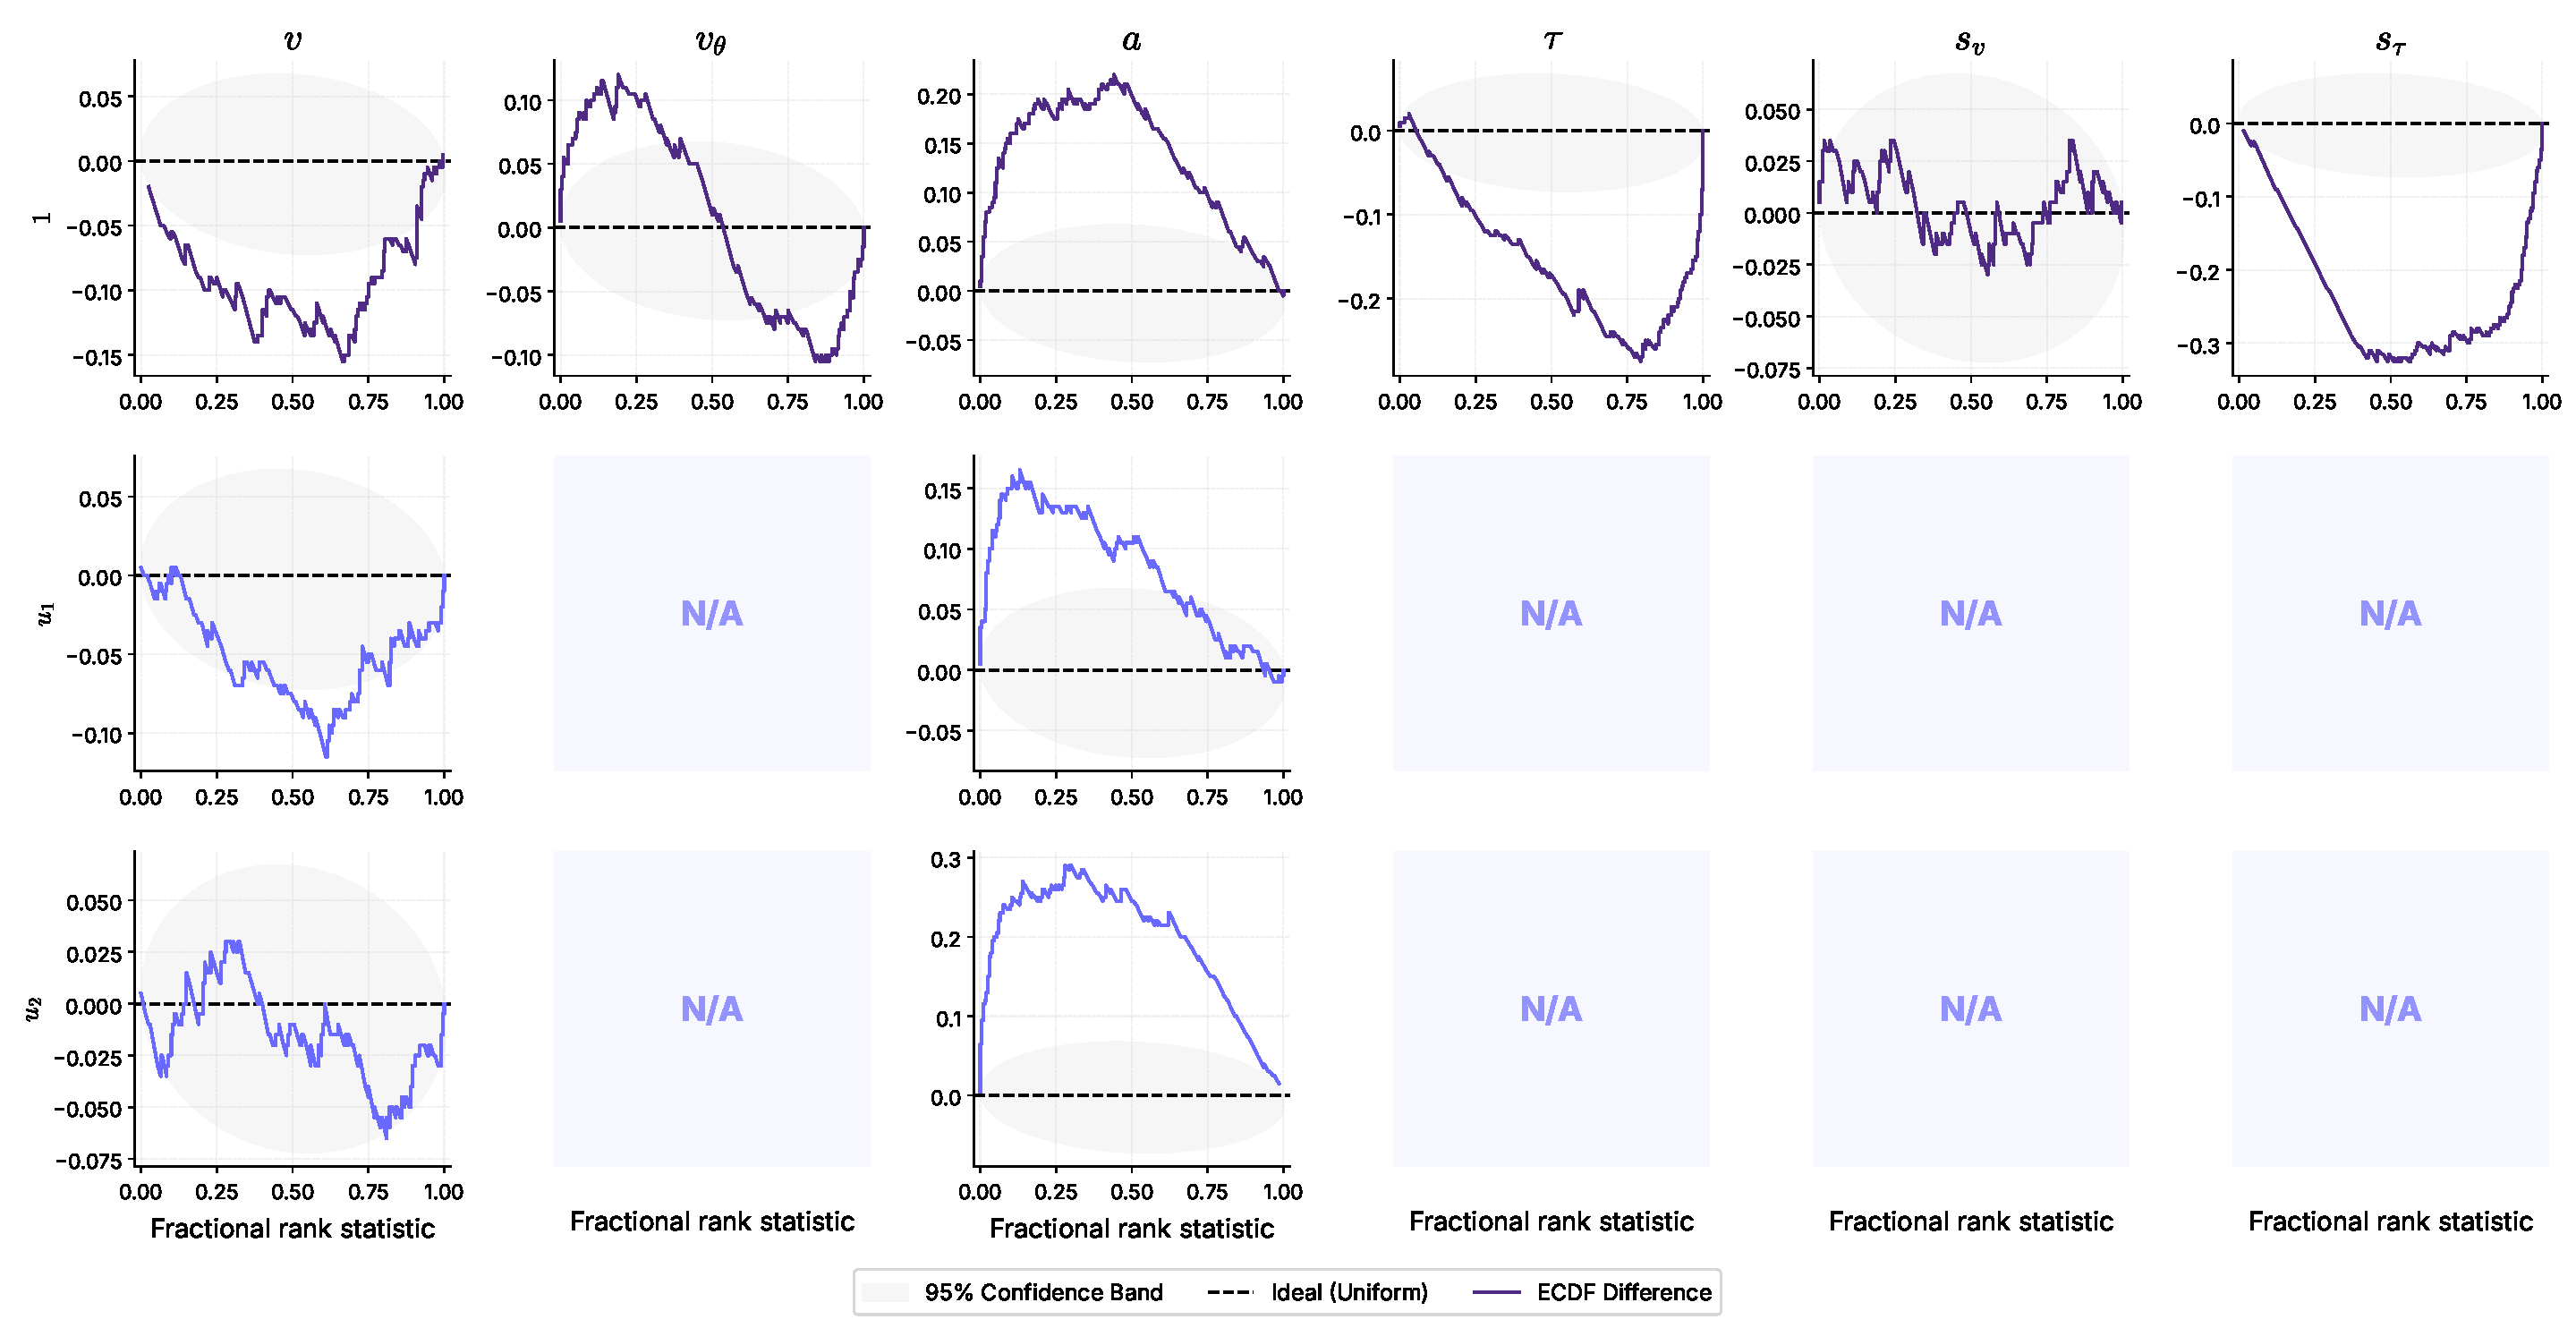
\includegraphics[width=\textwidth,height=0.3\textheight,keepaspectratio]{finetuned/cdm/regressed/ecdf.pdf}
    \caption{Calibration (ECDF)}
  \end{subfigure}\\[1ex]
  \begin{subfigure}{\textwidth}\centering
    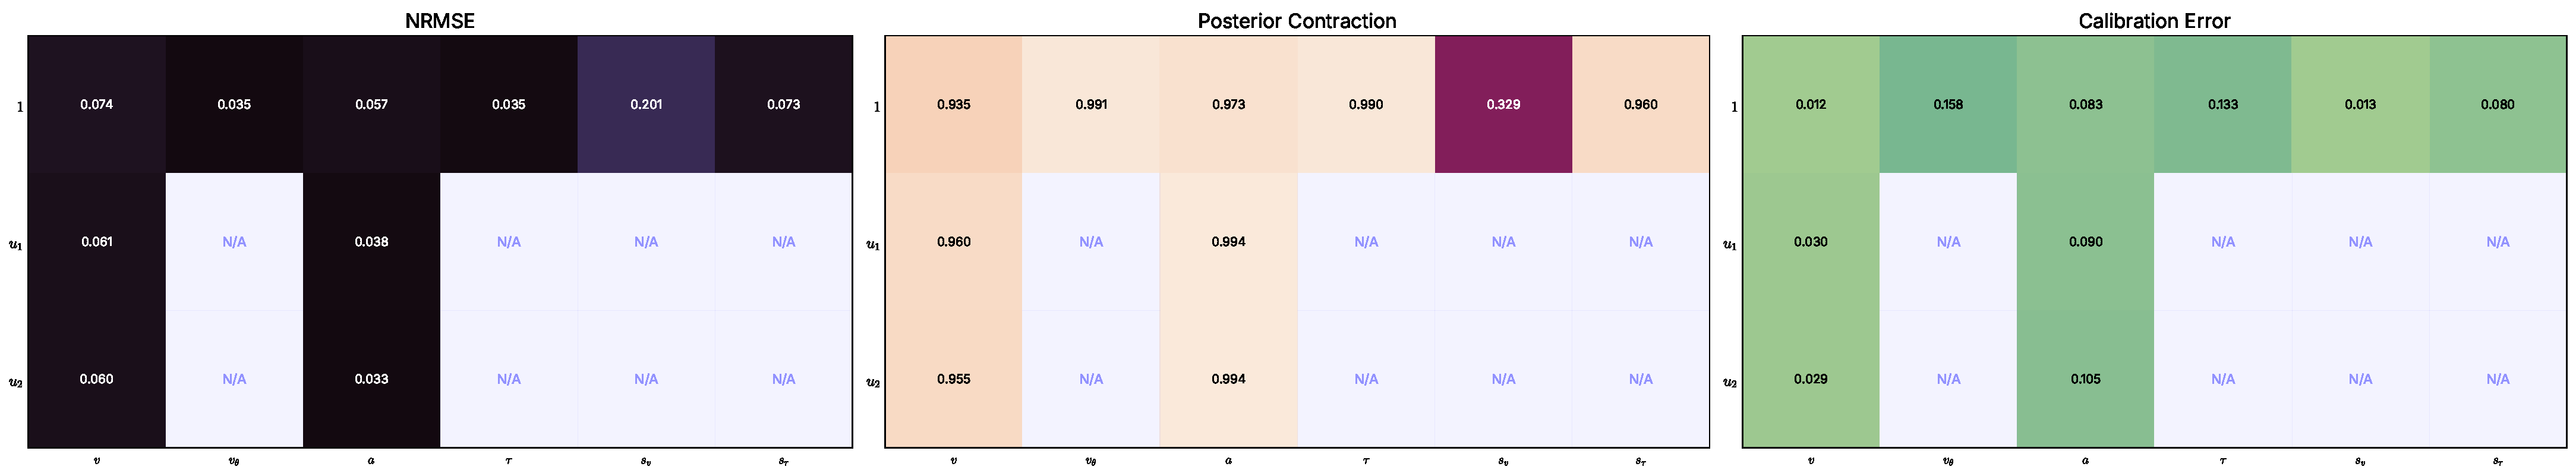
\includegraphics[width=\textwidth]{finetuned/cdm/regressed/metrics.pdf}
    \caption{Metrics}
  \end{subfigure}
  \caption{\textbf{After fine-tuning: CDM, \emph{regressed} design.} (a) Recovery, (b) calibration, (c) metrics. $v$ and $a$ carry slopes on $u_1$ and $u_2$ (10 coefficients shown). As in Figure~\ref{fig:app3-finetuned-lba-intercept-only}; before fine-tuning: Figure~\ref{fig:app1-cdm-regressed-cf}.}
  \label{fig:app3-finetuned-cdm-regressed}
\end{figure}

\begin{figure}[p]
  \centering
  \begin{subfigure}{\textwidth}\centering
    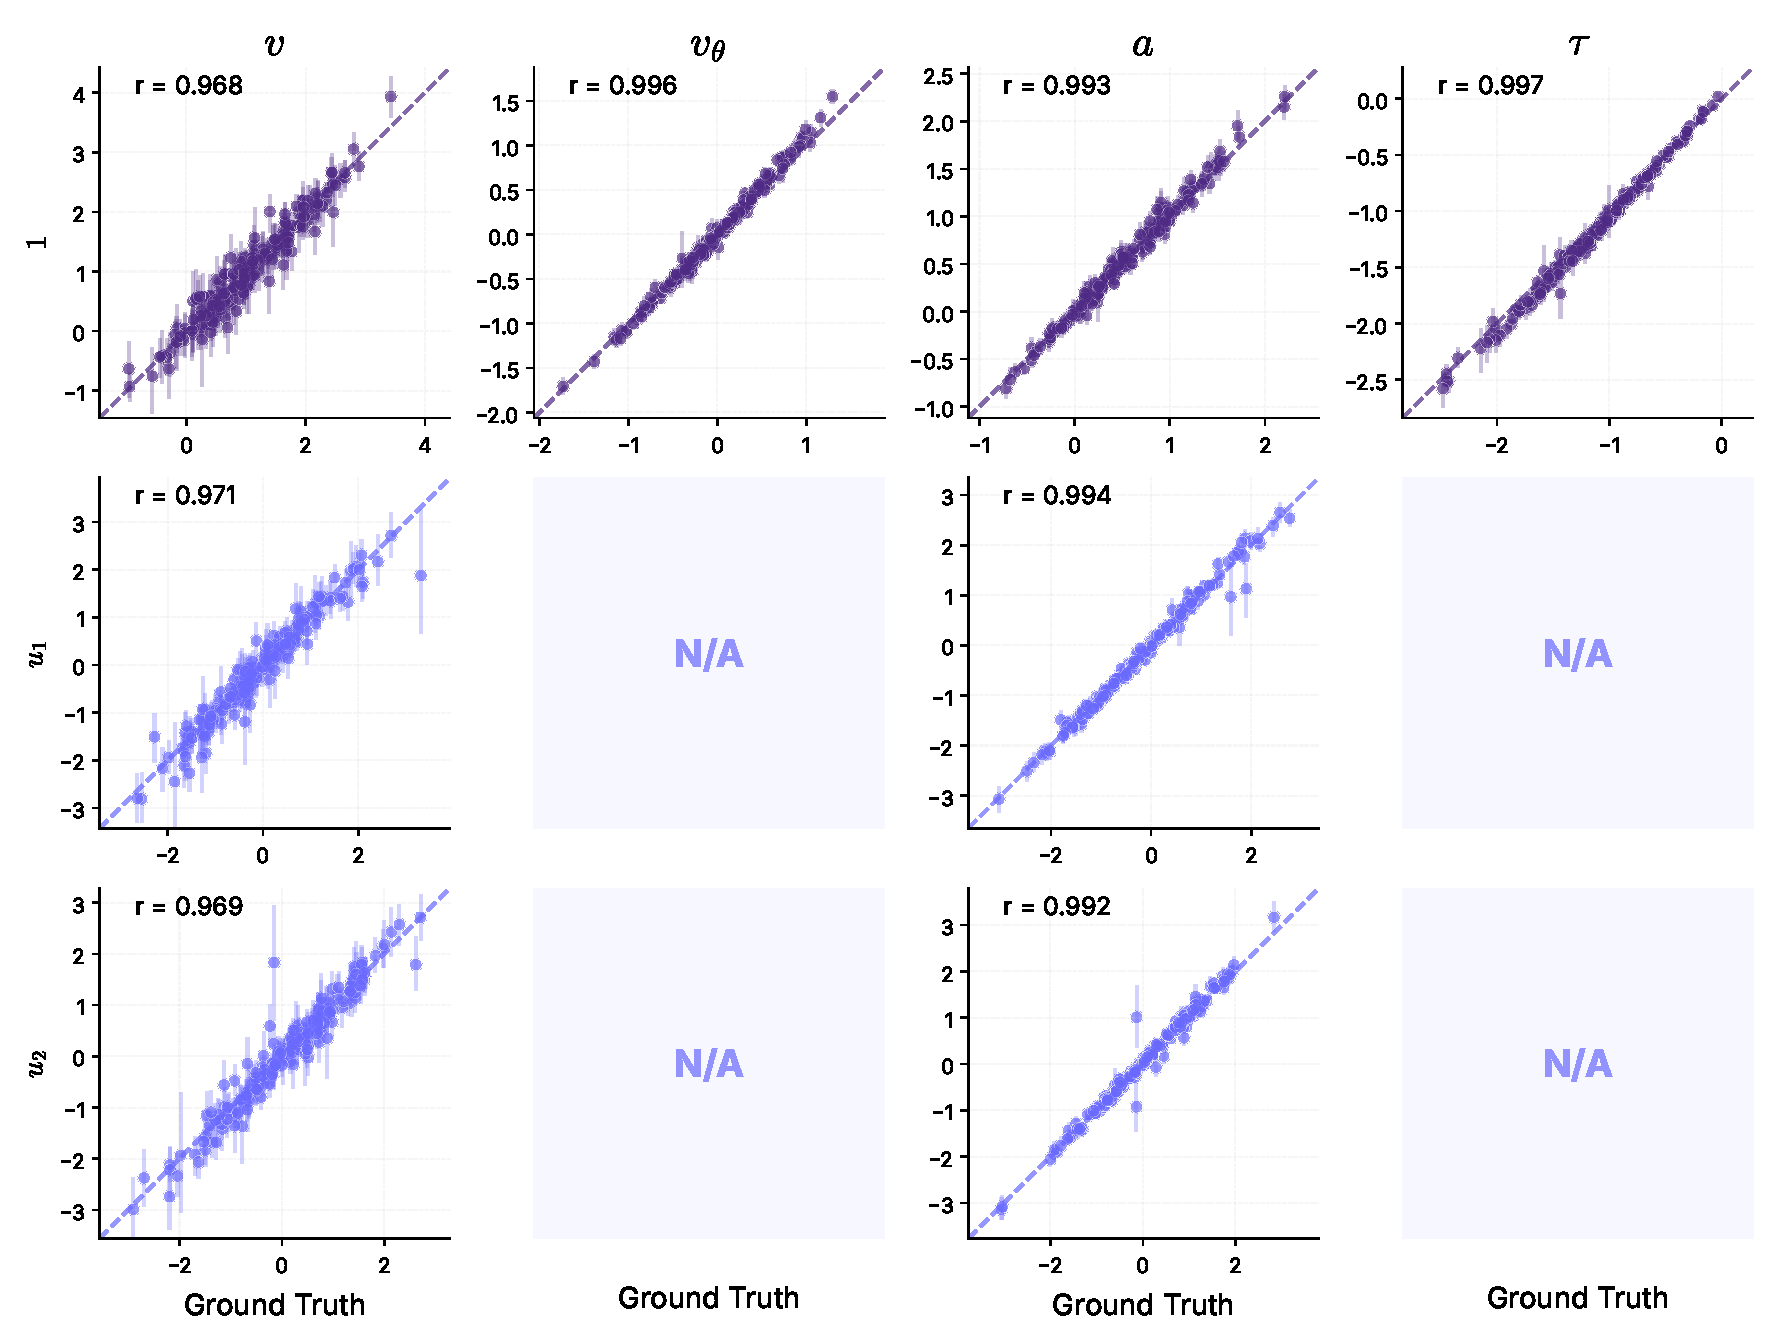
\includegraphics[width=\textwidth,height=0.3\textheight,keepaspectratio]{finetuned/cdm/fixed_regressed/recovery.pdf}
    \caption{Recovery}
  \end{subfigure}\\[1ex]
  \begin{subfigure}{\textwidth}\centering
    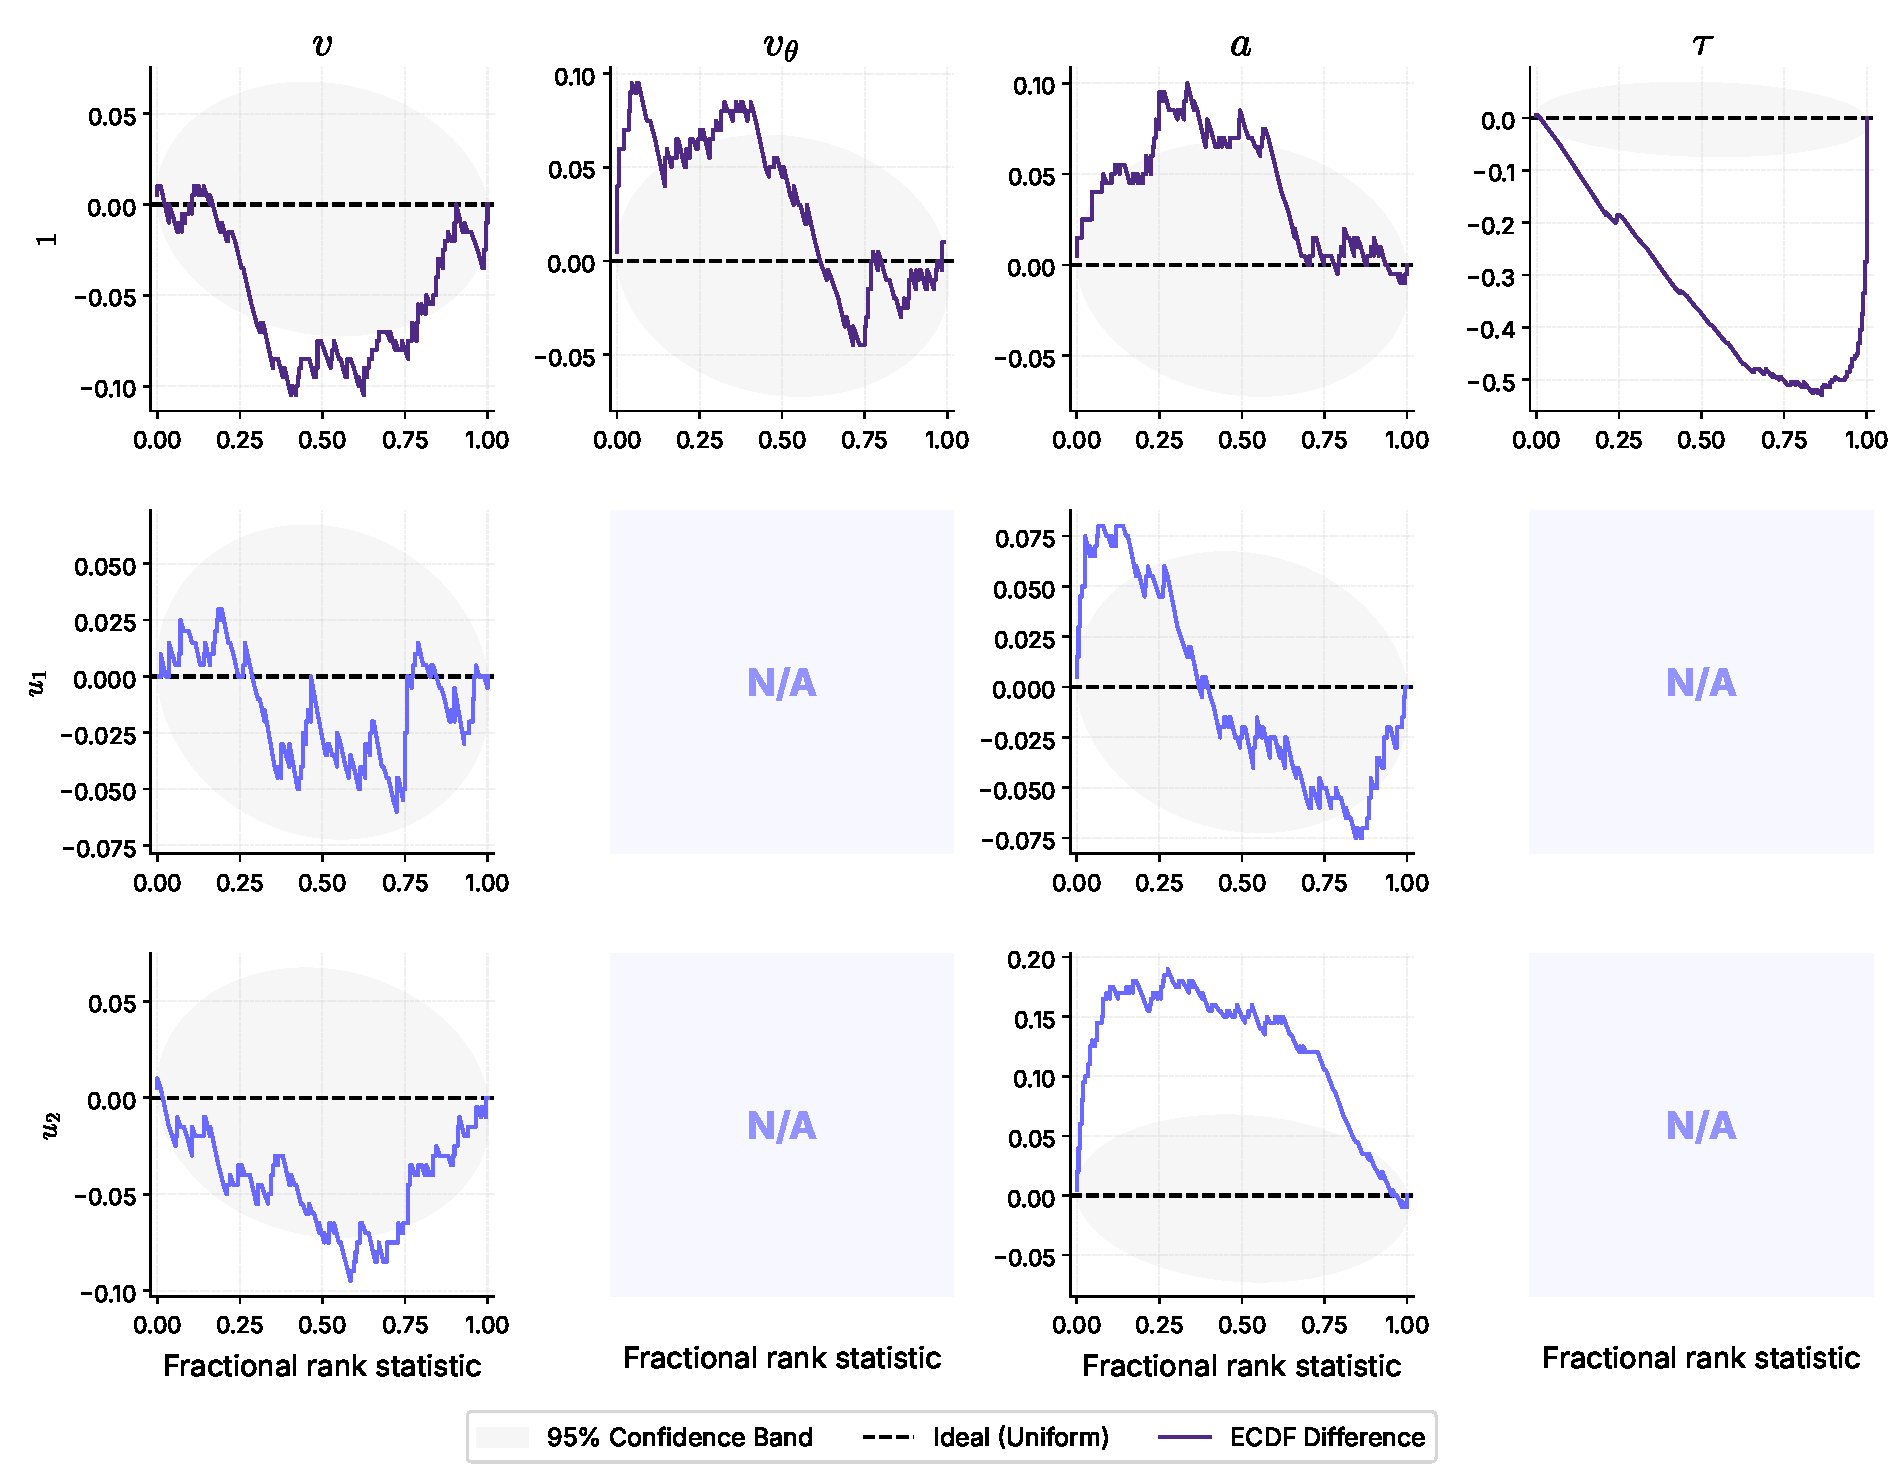
\includegraphics[width=\textwidth,height=0.3\textheight,keepaspectratio]{finetuned/cdm/fixed_regressed/ecdf.pdf}
    \caption{Calibration (ECDF)}
  \end{subfigure}\\[1ex]
  \begin{subfigure}{\textwidth}\centering
    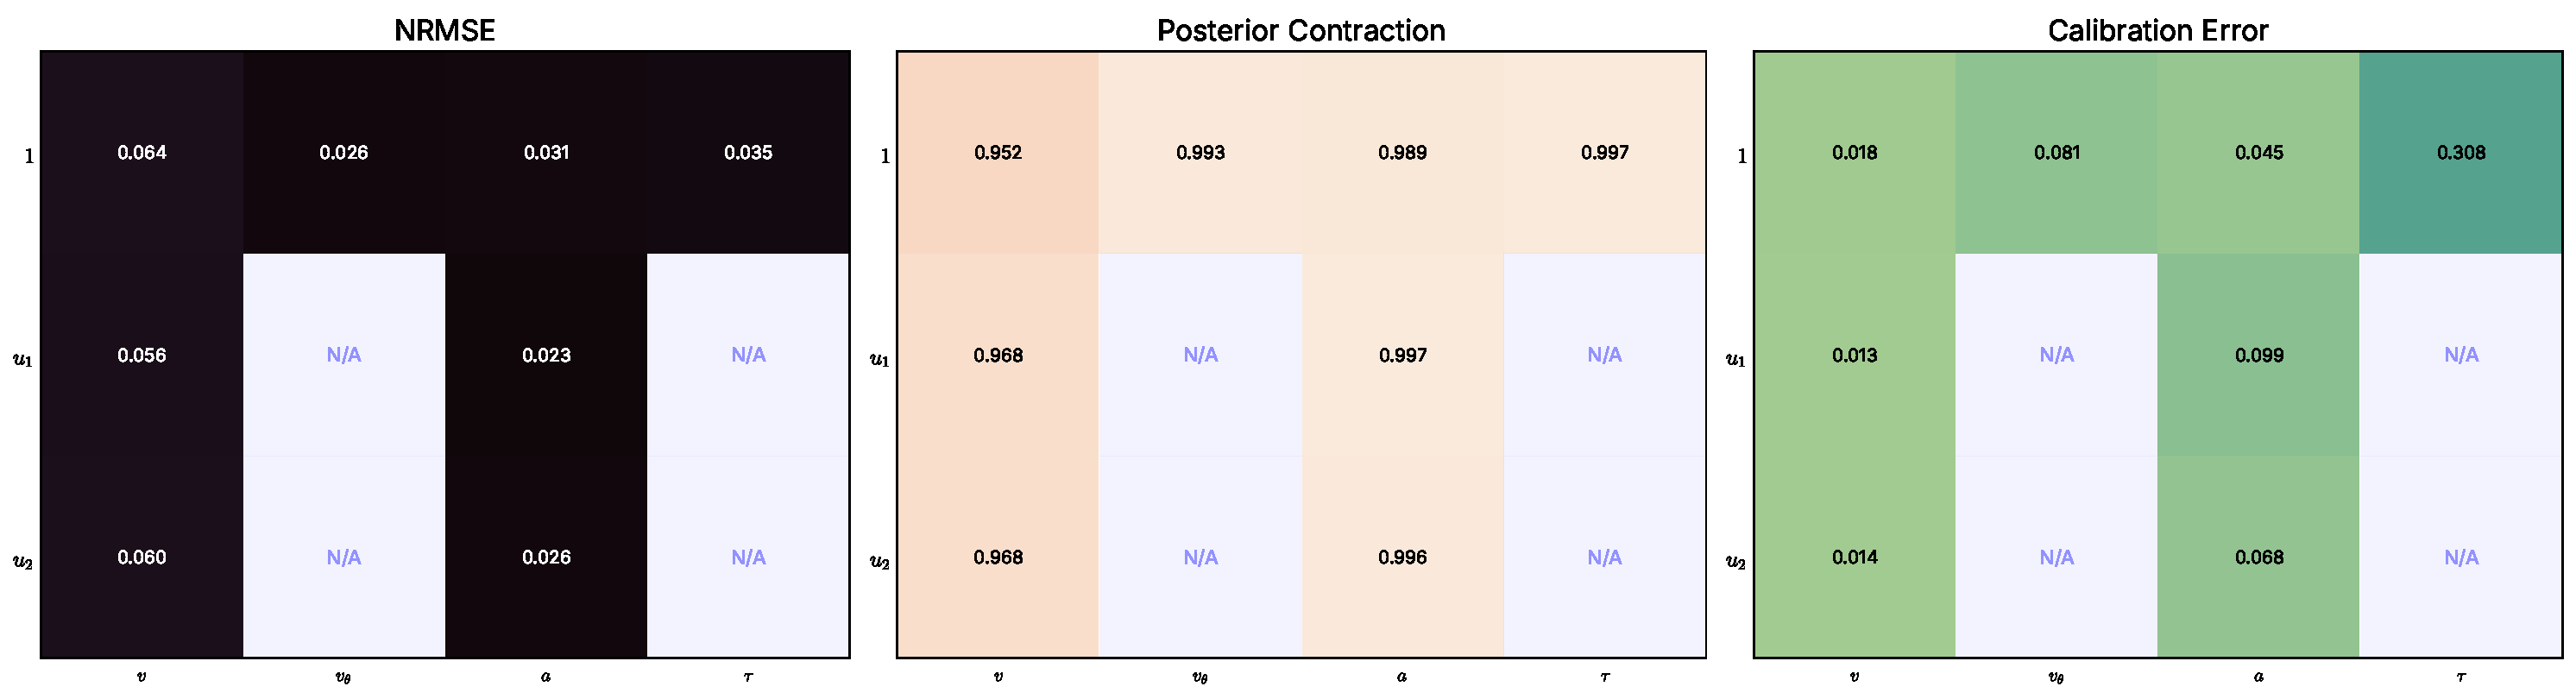
\includegraphics[width=\textwidth]{finetuned/cdm/fixed_regressed/metrics.pdf}
    \caption{Metrics}
  \end{subfigure}
  \caption{\textbf{After fine-tuning: CDM, \emph{fixed + regressed} design.} (a) Recovery, (b) calibration, (c) metrics. $s_v$ and $s_\tau$ are fixed at 0 and not estimated; $v$ and $a$ carry slopes on $u_1$ and $u_2$ (8 coefficients shown). As in Figure~\ref{fig:app3-finetuned-lba-intercept-only}; before fine-tuning: Figure~\ref{fig:app1-cdm-fixed-regressed-cf}.}
  \label{fig:app3-finetuned-cdm-fixed-regressed}
\end{figure}

\begin{figure}[p]
  \centering
  \begin{subfigure}{\textwidth}\centering
    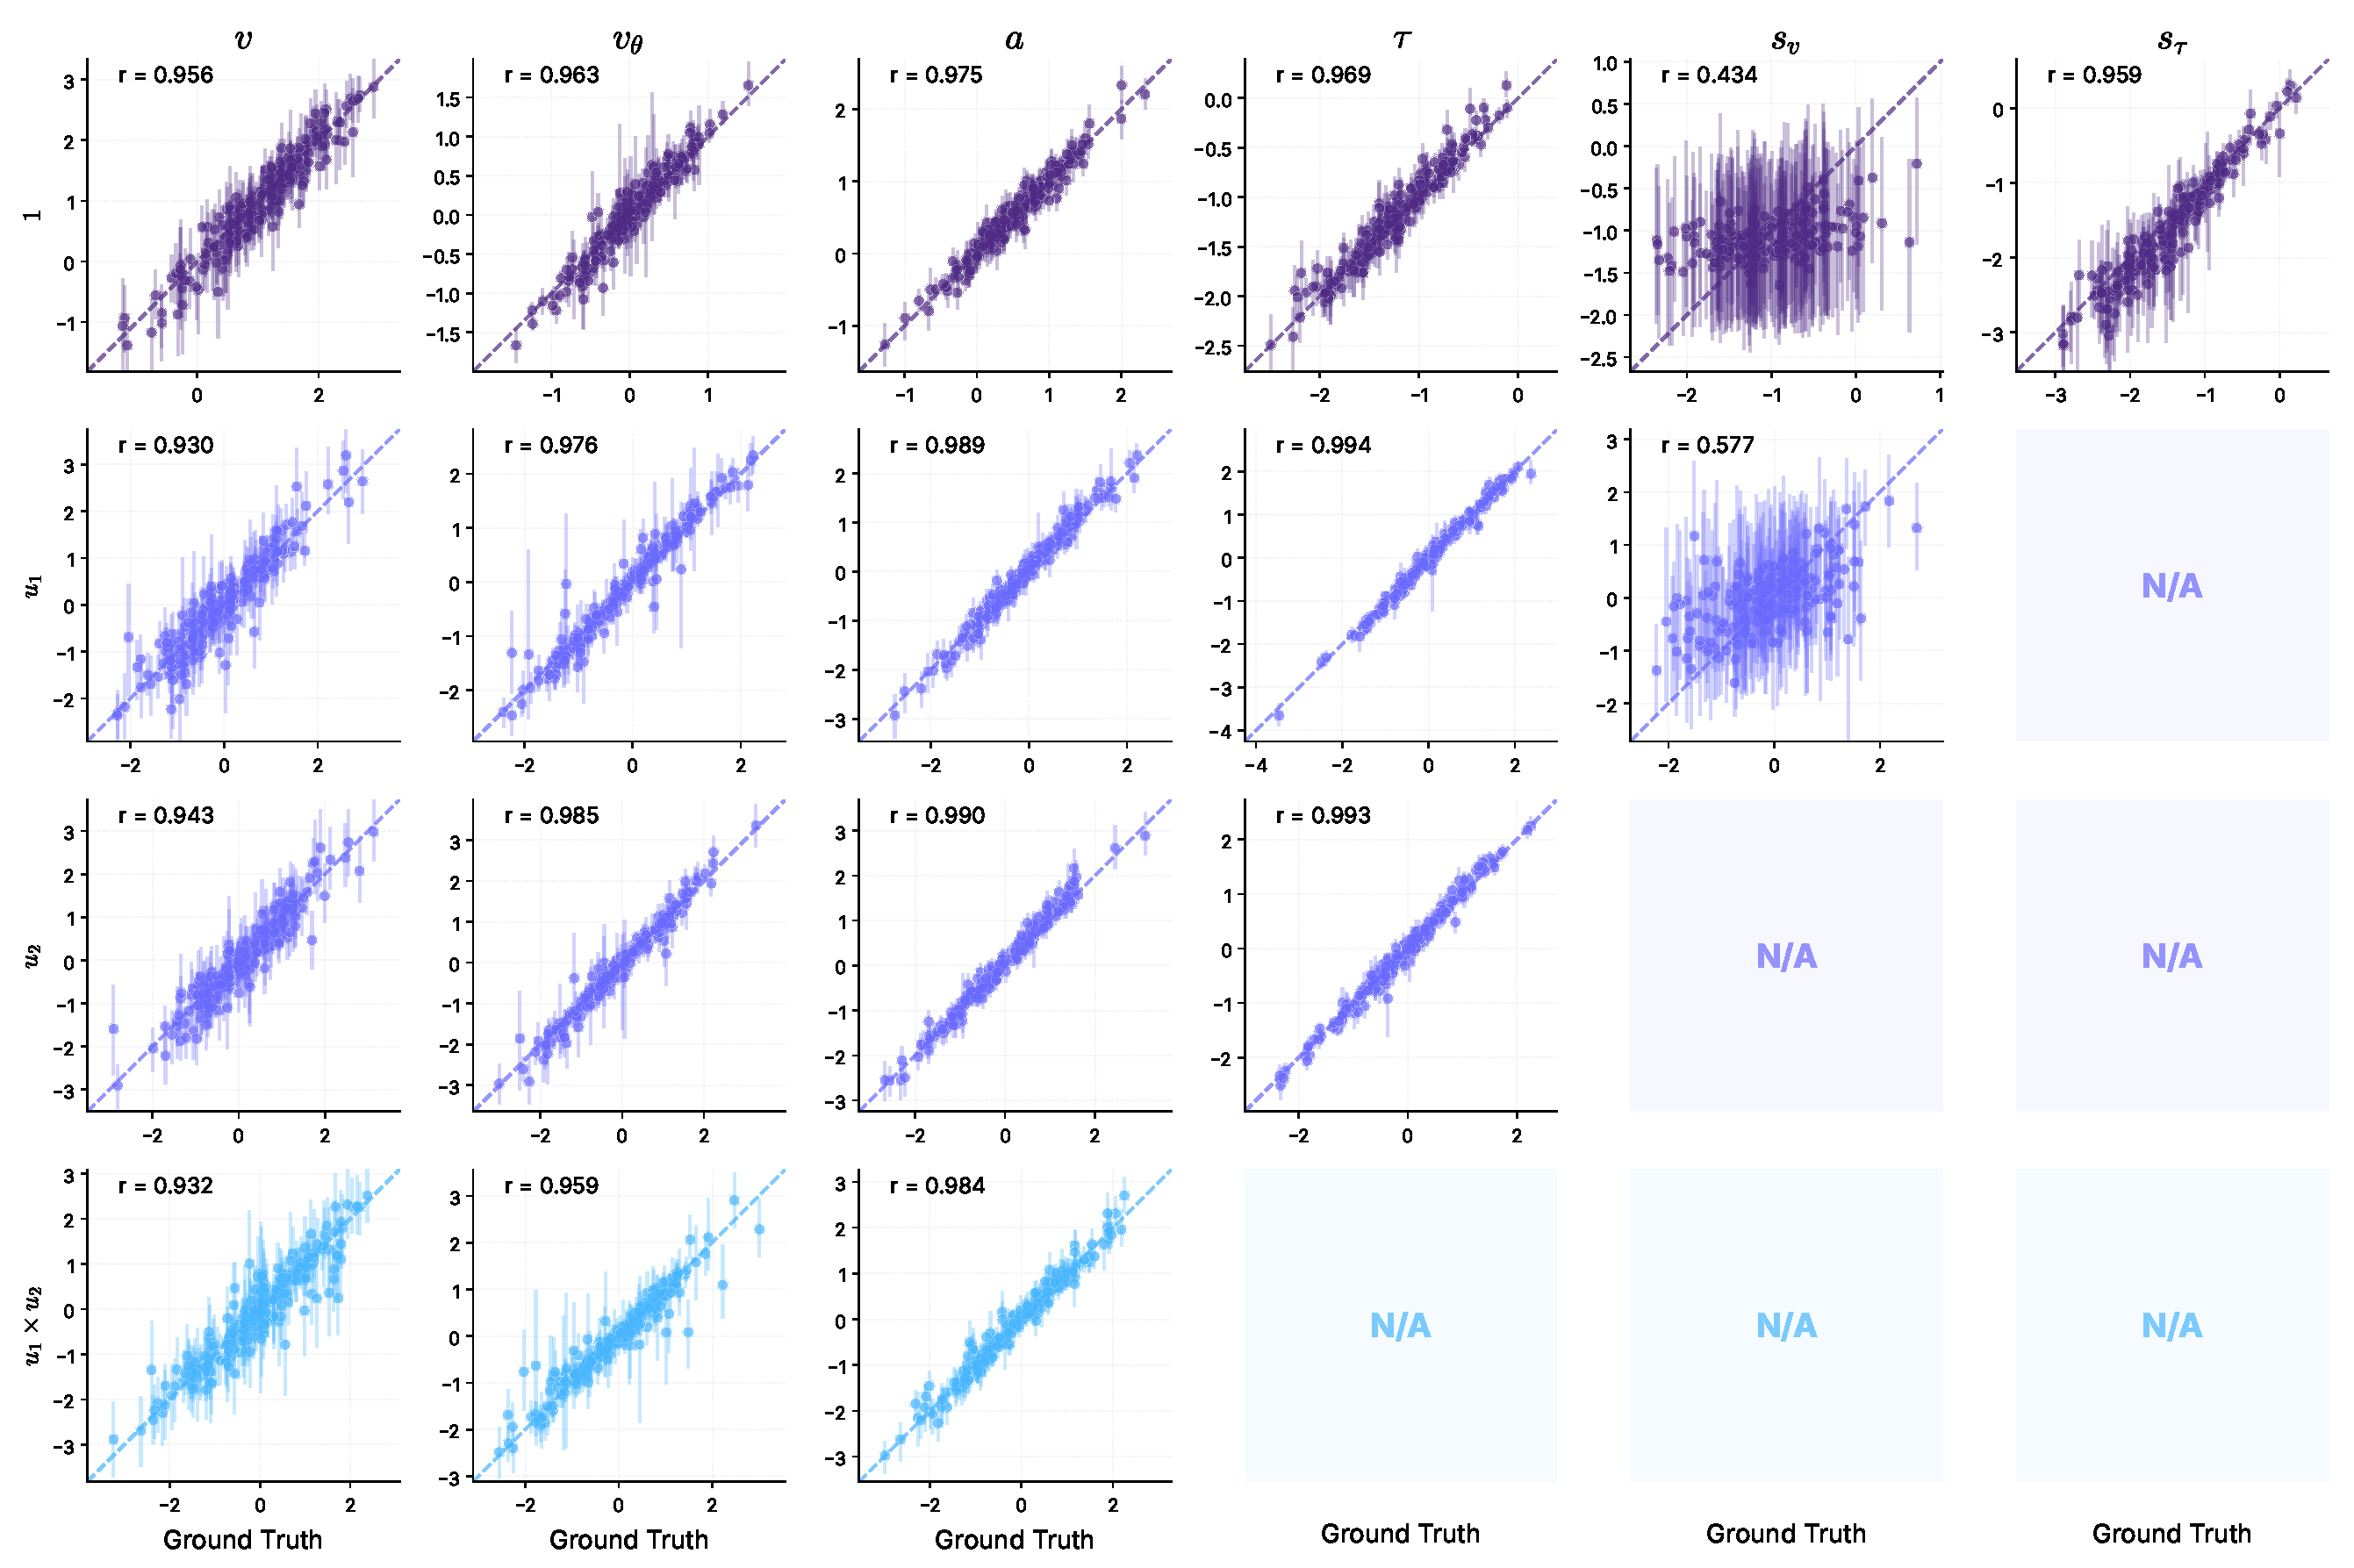
\includegraphics[width=\textwidth,height=0.3\textheight,keepaspectratio]{finetuned/cdm/interaction/recovery.pdf}
    \caption{Recovery}
  \end{subfigure}\\[1ex]
  \begin{subfigure}{\textwidth}\centering
    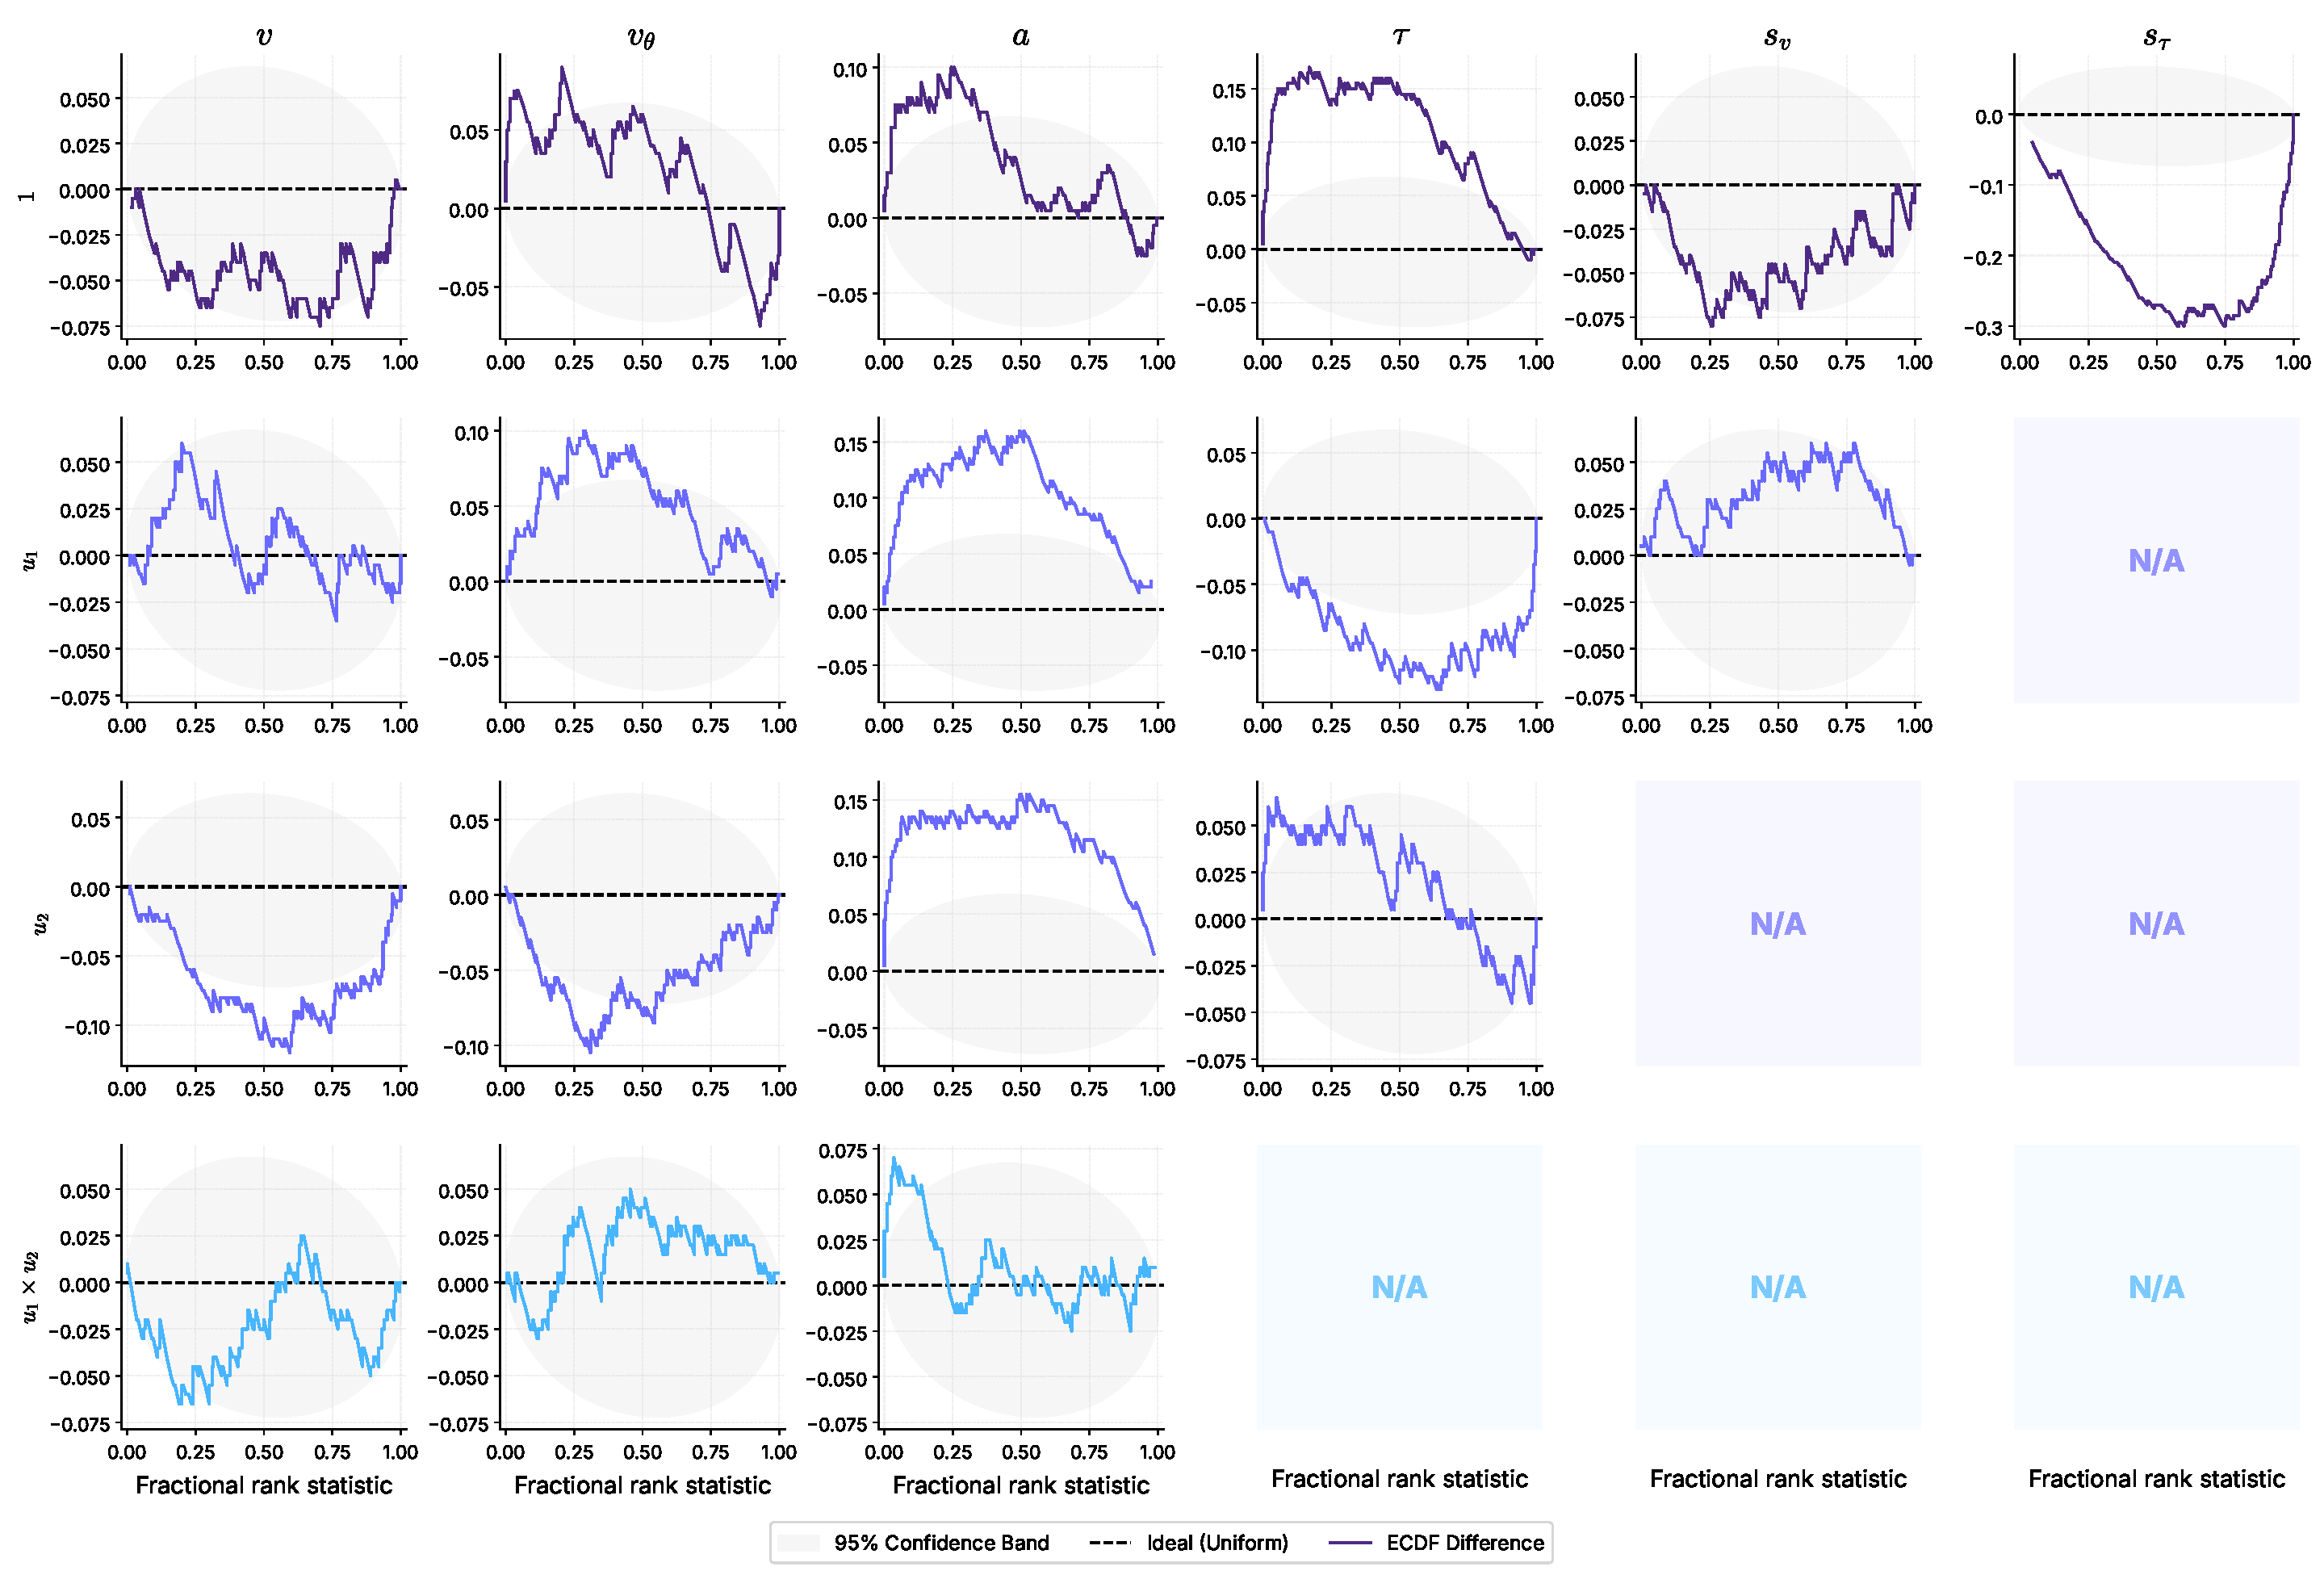
\includegraphics[width=\textwidth,height=0.3\textheight,keepaspectratio]{finetuned/cdm/interaction/ecdf.pdf}
    \caption{Calibration (ECDF)}
  \end{subfigure}\\[1ex]
  \begin{subfigure}{\textwidth}\centering
    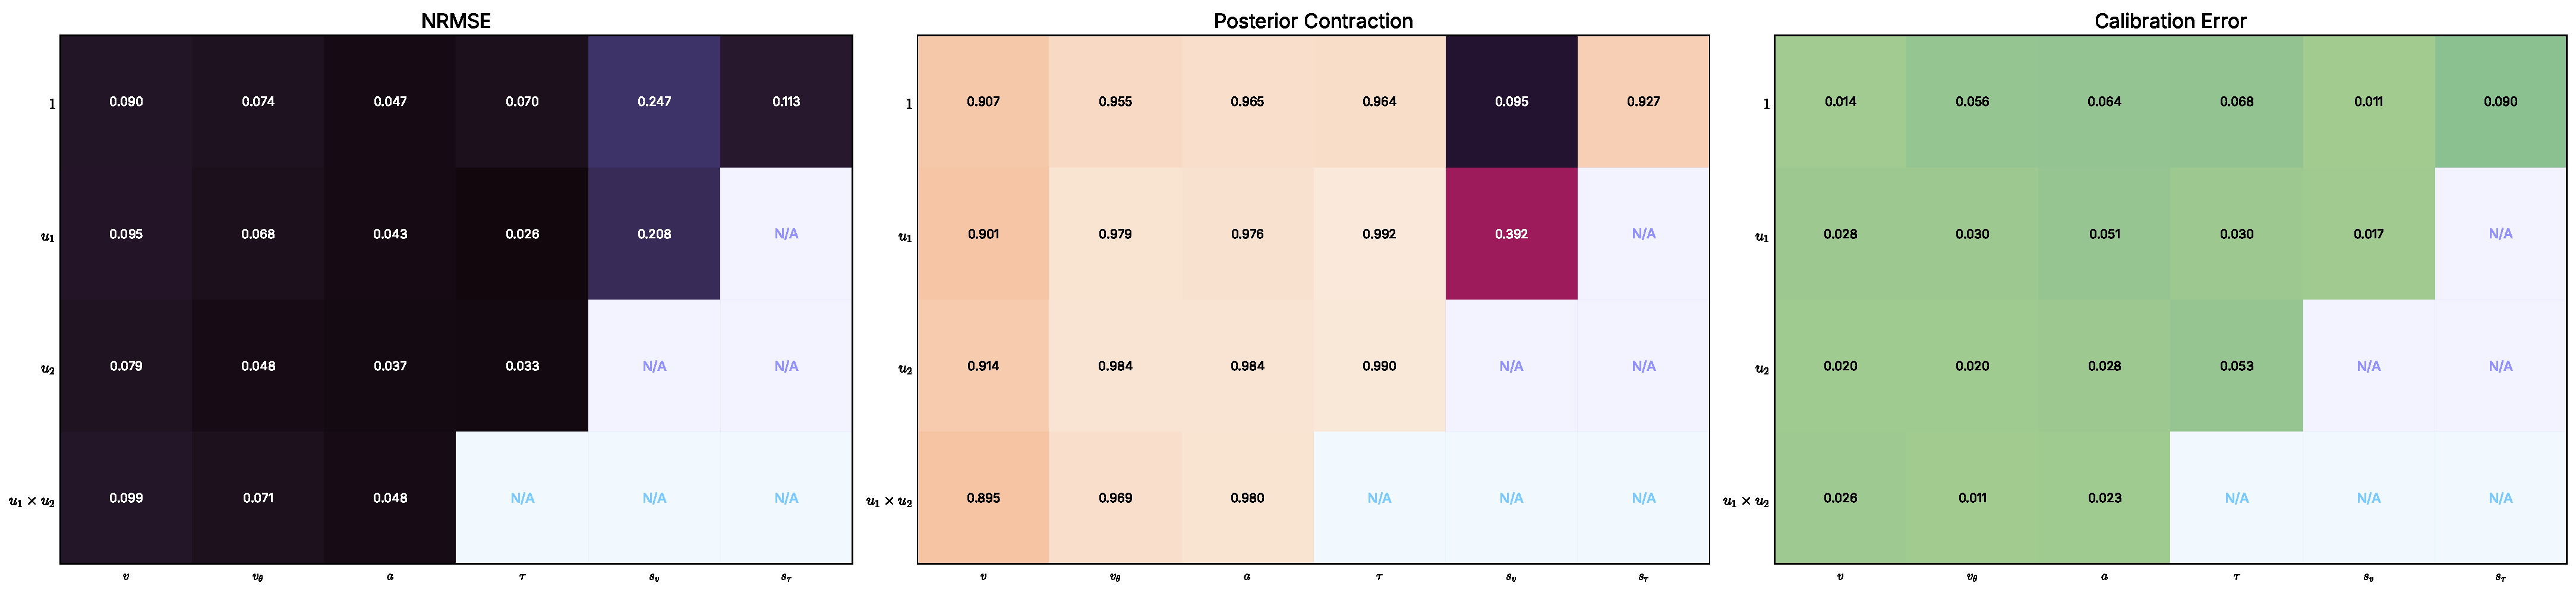
\includegraphics[width=\textwidth]{finetuned/cdm/interaction/metrics.pdf}
    \caption{Metrics}
  \end{subfigure}
  \caption{\textbf{After fine-tuning: CDM, \emph{interaction} design.} (a) Recovery, (b) calibration, (c) metrics. $v$, $v_\theta$, $a$, $\tau$ and $s_v$ carry slopes on $u_1$; $v$, $v_\theta$, $a$ and $\tau$ carry slopes on $u_2$; $v$, $v_\theta$ and $a$ on the product $u_1 u_2$ (18 coefficients shown). As in Figure~\ref{fig:app3-finetuned-lba-intercept-only}; before fine-tuning: Figure~\ref{fig:app1-cdm-interaction-cf}.}
  \label{fig:app3-finetuned-cdm-interaction}
\end{figure}

\begin{figure}[p]
  \centering
  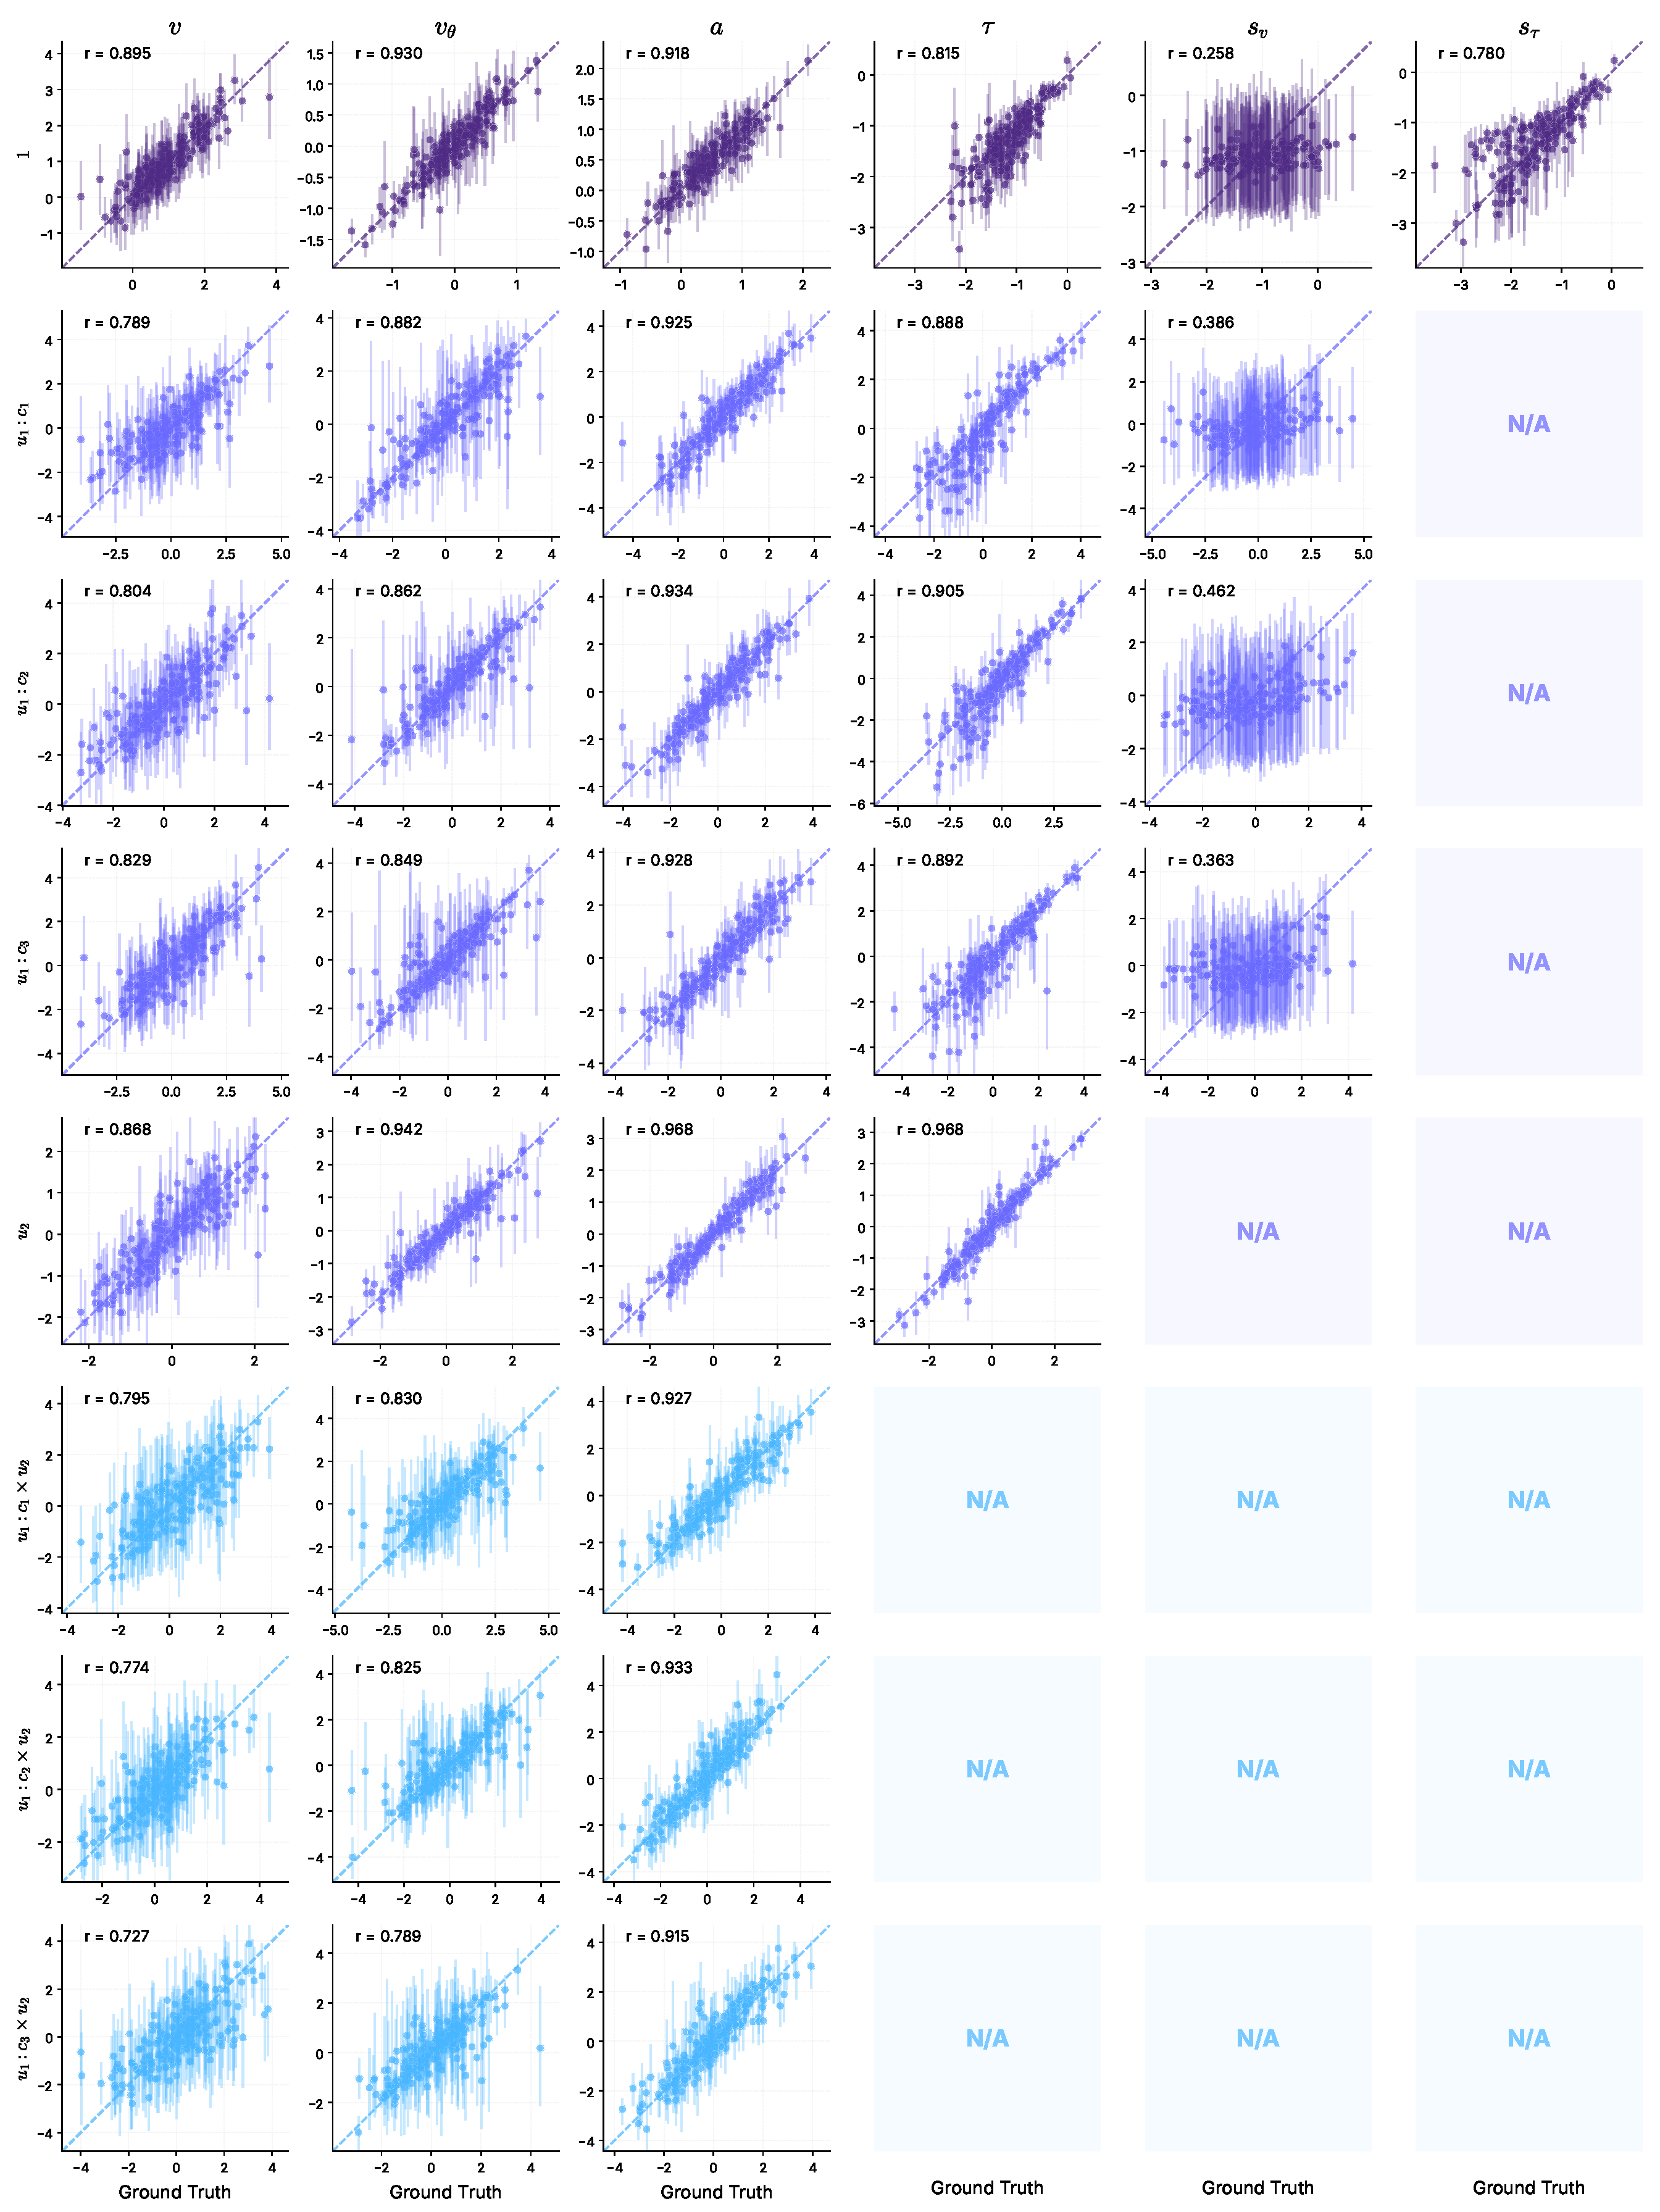
\includegraphics[width=\textwidth,height=0.82\textheight,keepaspectratio]{finetuned/cdm/mixed_predictor/recovery.pdf}
  \caption{\textbf{Parameter recovery, CDM after fine-tuning, mixed-predictor design.} $v$, $v_\theta$, $a$, $\tau$ and $s_v$ carry effects of the four-level $u_1$; $v$, $v_\theta$, $a$ and $\tau$ slopes on $u_2$; $v$, $v_\theta$ and $a$ the interaction (34 coefficients shown). Datasets simulated for this design (no shared benchmark file exists); design as in Figure~\ref{fig:app1-ddm-mixed-predictor-recovery}, encoding as in the top panel of Figure~\ref{fig:app1-ddm-intercept-only-cf}.}
  \label{fig:app3-finetuned-cdm-mixed-predictor-recovery}
\end{figure}

\begin{figure}[p]
  \centering
  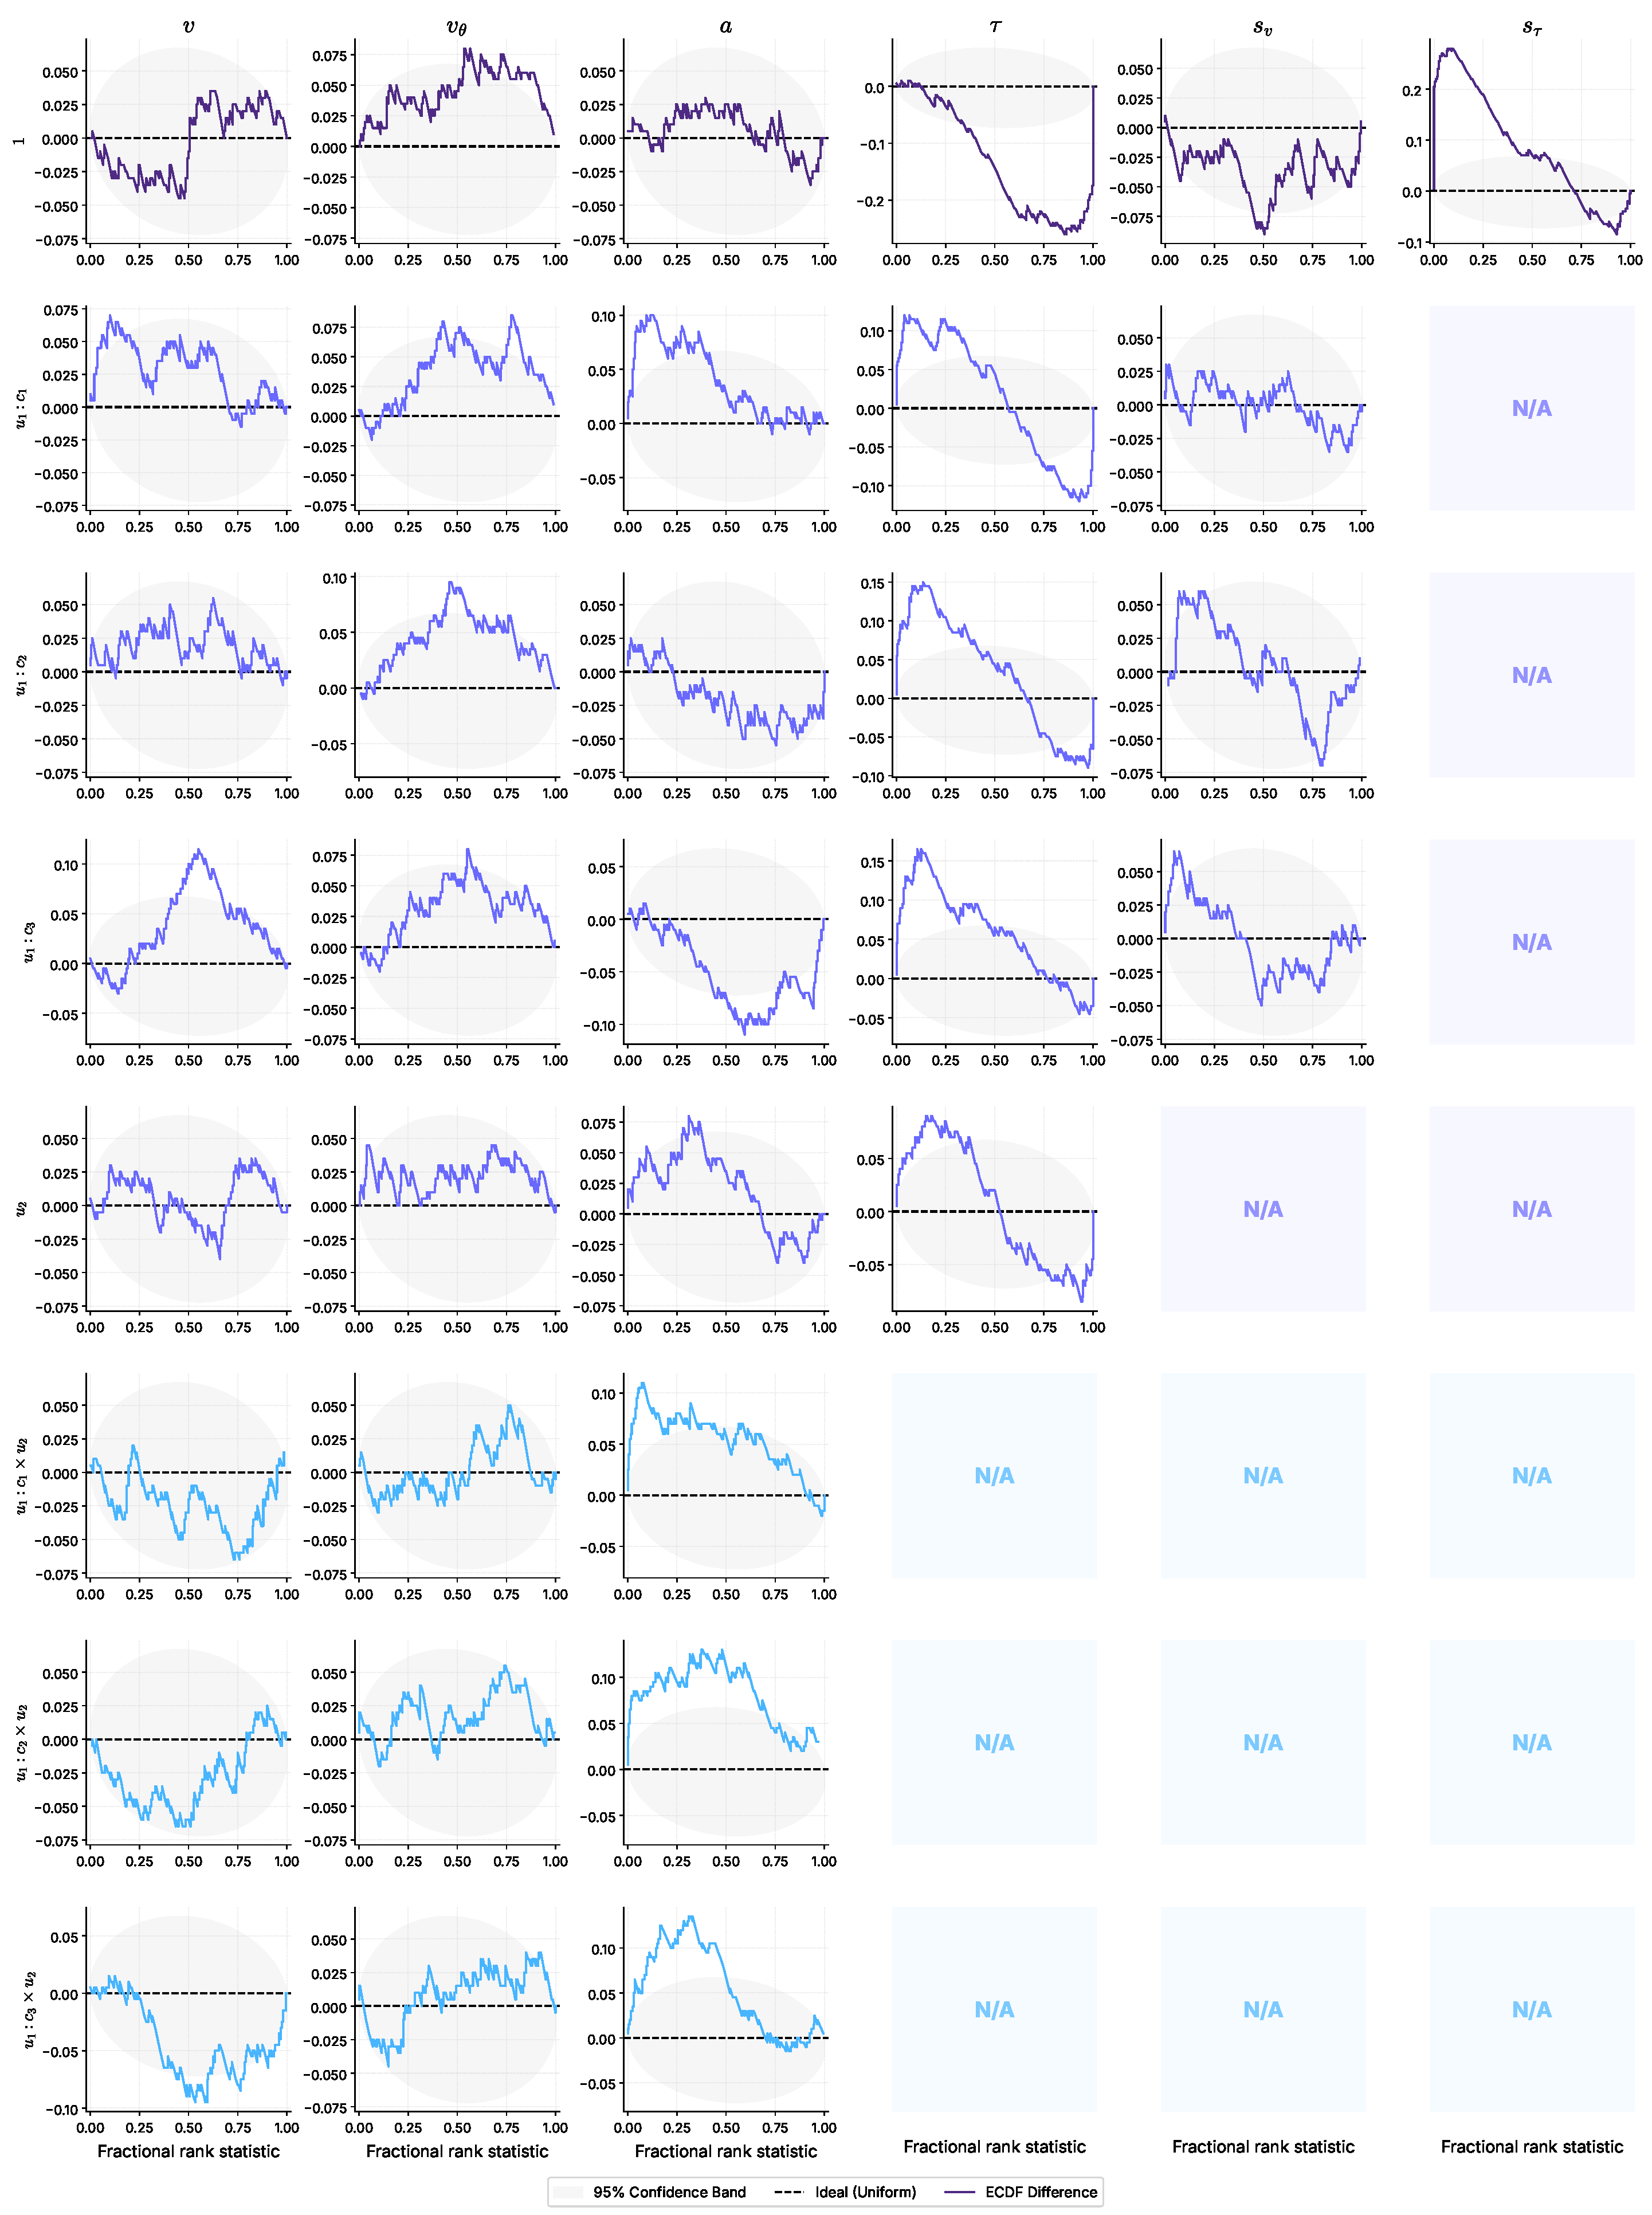
\includegraphics[width=\textwidth,height=0.82\textheight,keepaspectratio]{finetuned/cdm/mixed_predictor/ecdf.pdf}
  \caption{\textbf{Simulation-based calibration, CDM after fine-tuning, mixed-predictor design.} $v$, $v_\theta$, $a$, $\tau$ and $s_v$ carry effects of the four-level $u_1$; $v$, $v_\theta$, $a$ and $\tau$ slopes on $u_2$; $v$, $v_\theta$ and $a$ the interaction (34 coefficients shown). Datasets simulated for this design (no shared benchmark file exists); design as in Figure~\ref{fig:app1-ddm-mixed-predictor-recovery}, encoding as in the middle panel of Figure~\ref{fig:app1-ddm-intercept-only-cf}.}
  \label{fig:app3-finetuned-cdm-mixed-predictor-ecdf}
\end{figure}

\begin{figure}[p]
  \centering
  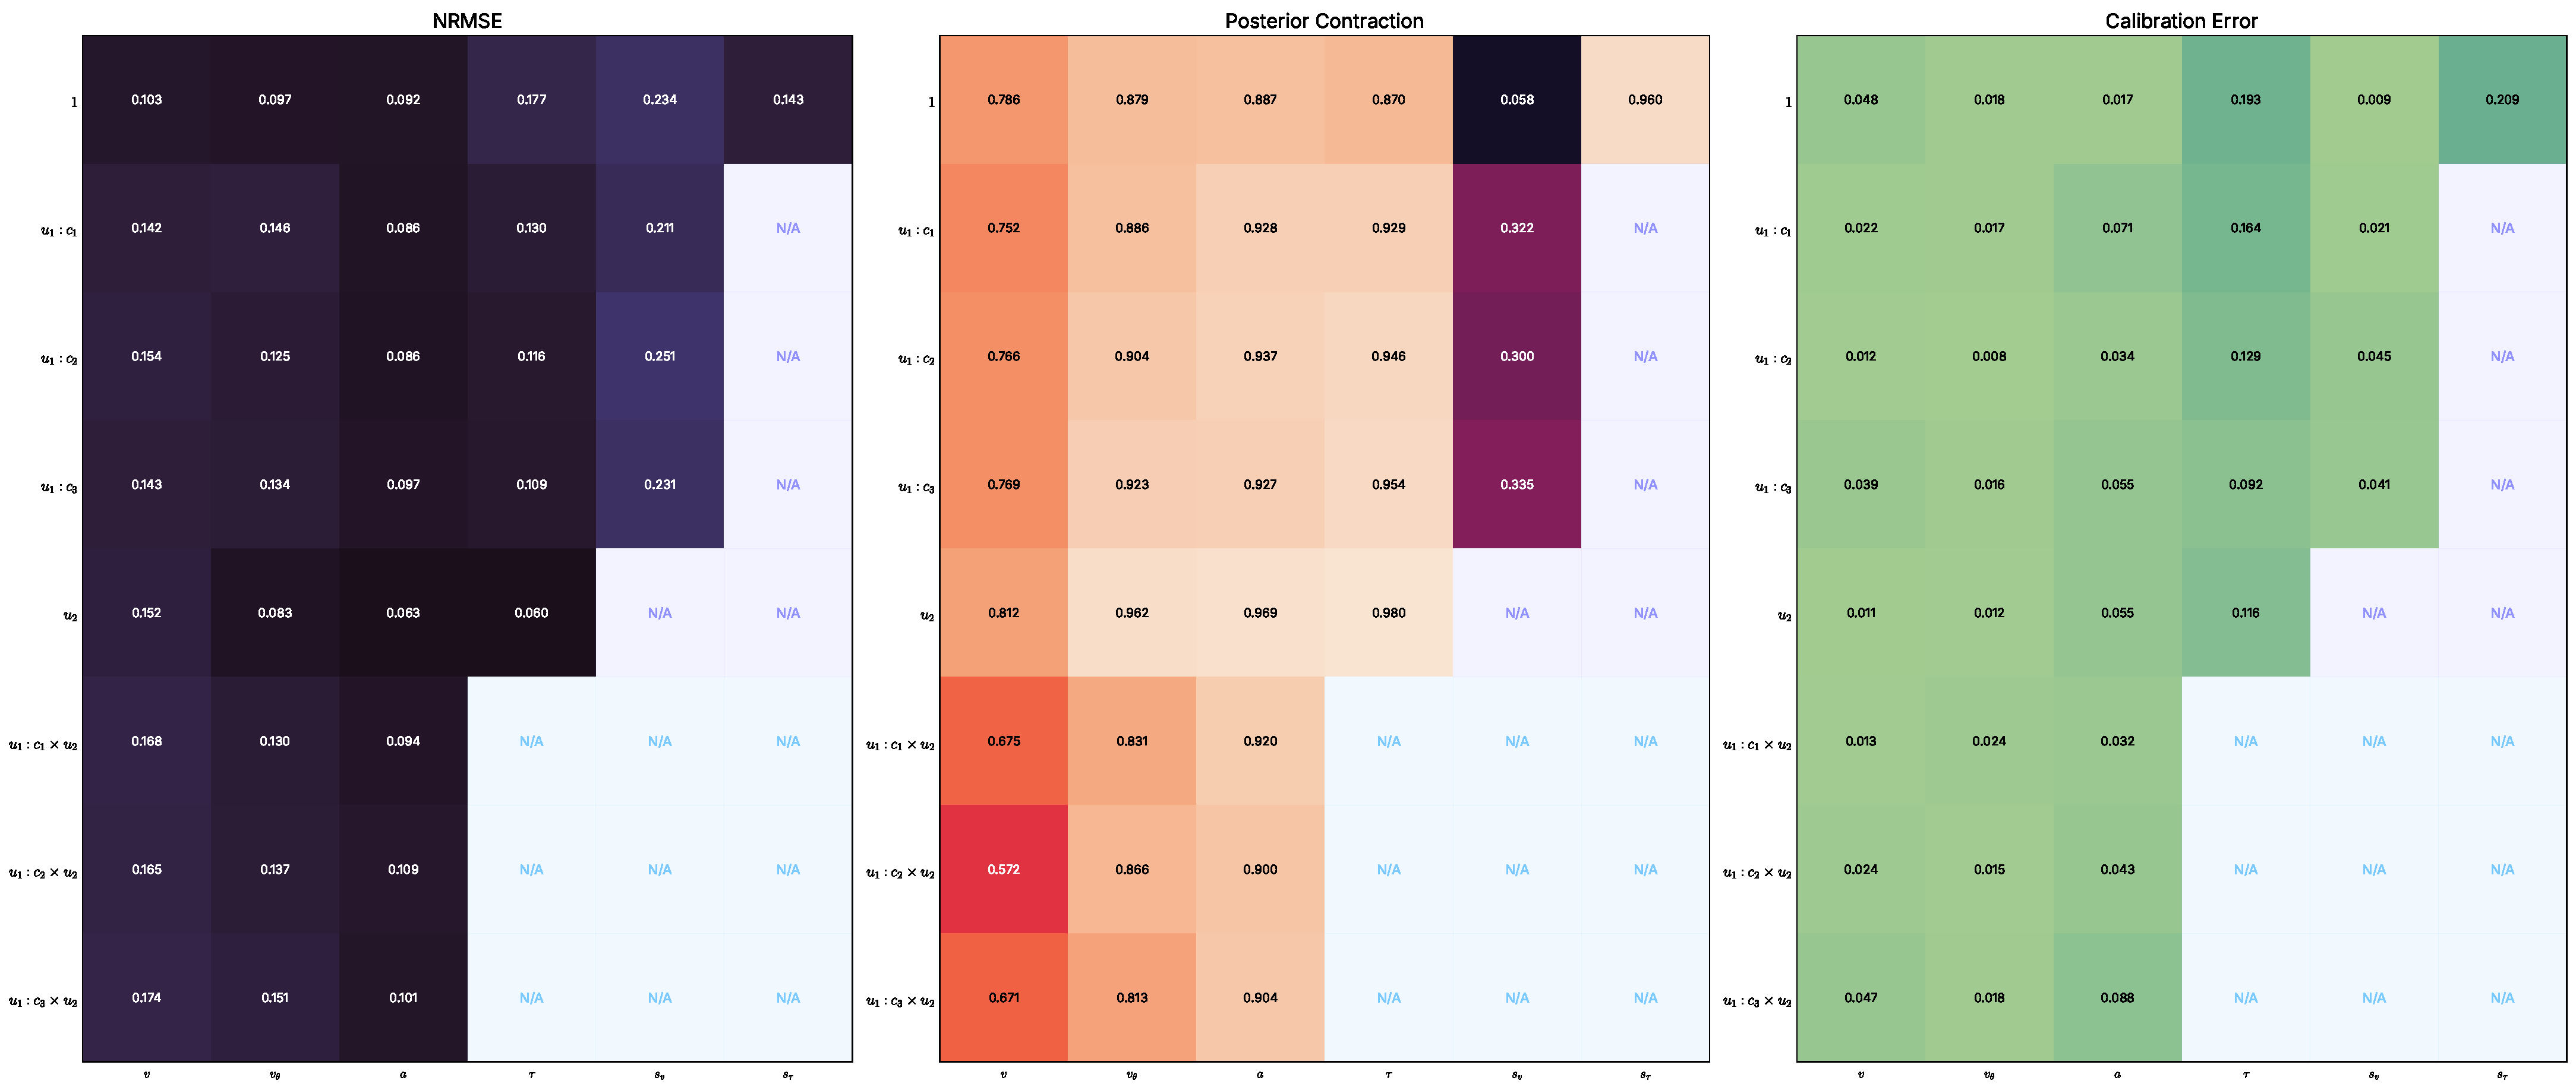
\includegraphics[width=\textwidth,height=0.82\textheight,keepaspectratio]{finetuned/cdm/mixed_predictor/metrics.pdf}
  \caption{\textbf{Summary metrics, CDM after fine-tuning, mixed-predictor design.} $v$, $v_\theta$, $a$, $\tau$ and $s_v$ carry effects of the four-level $u_1$; $v$, $v_\theta$, $a$ and $\tau$ slopes on $u_2$; $v$, $v_\theta$ and $a$ the interaction (34 coefficients shown). Datasets simulated for this design (no shared benchmark file exists); design as in Figure~\ref{fig:app1-ddm-mixed-predictor-recovery}, encoding as in the bottom panel of Figure~\ref{fig:app1-ddm-intercept-only-cf}.}
  \label{fig:app3-finetuned-cdm-mixed-predictor-metrics}
\end{figure}

% ── 3. change in recovery (Δr) ──

\begin{figure}[p]
  \centering
  \begin{subfigure}{\textwidth}\centering
    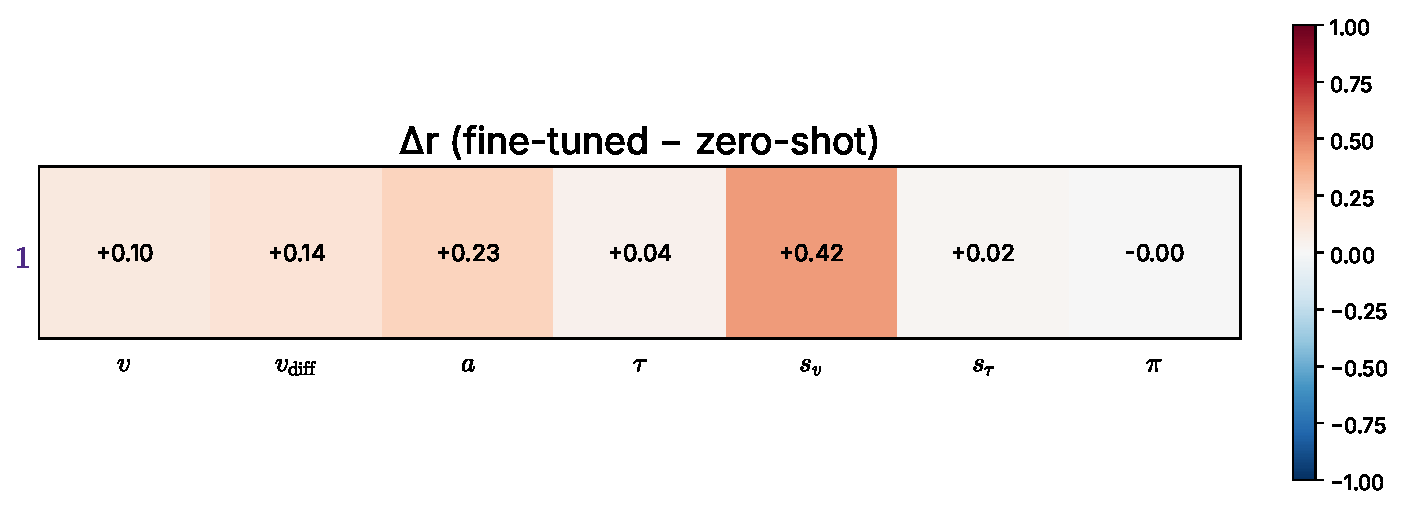
\includegraphics[width=\textwidth,height=0.18\textheight,keepaspectratio]{compare/lba/intercept_only_delta_r.pdf}
    \caption{}
  \end{subfigure}\\[0.5ex]
  \begin{subfigure}{\textwidth}\centering
    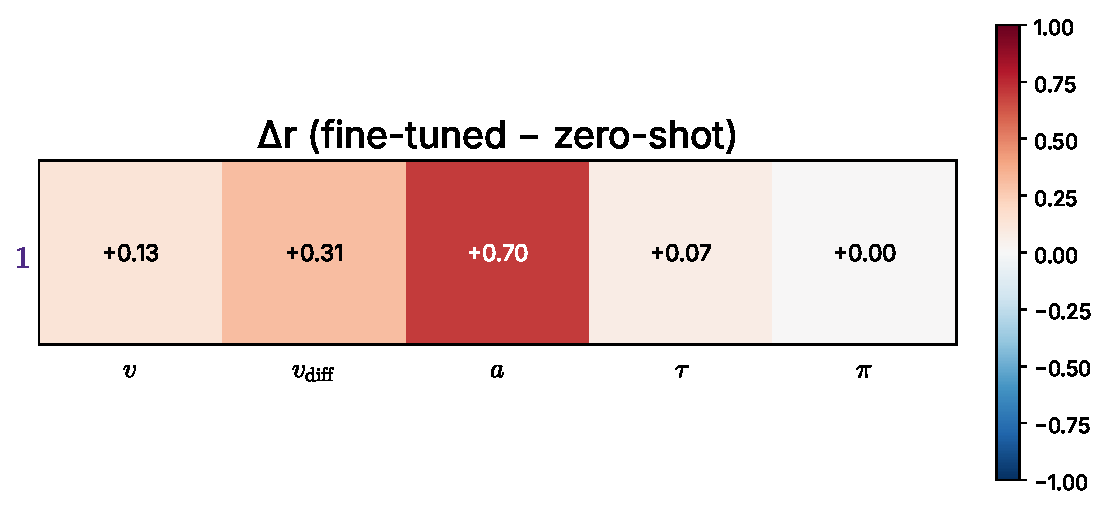
\includegraphics[width=\textwidth,height=0.18\textheight,keepaspectratio]{compare/lba/fixed_delta_r.pdf}
    \caption{}
  \end{subfigure}\\[0.5ex]
  \begin{subfigure}{\textwidth}\centering
    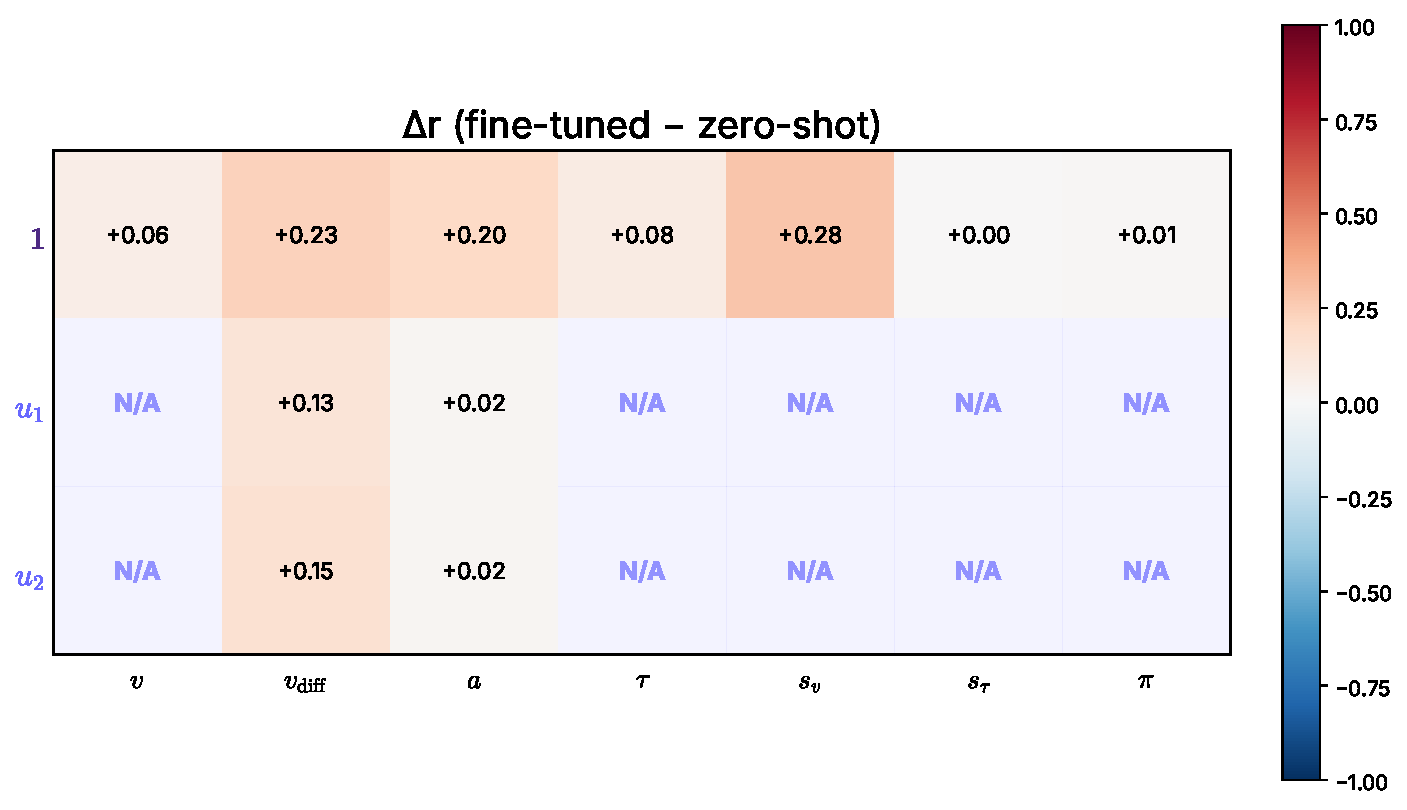
\includegraphics[width=\textwidth,height=0.18\textheight,keepaspectratio]{compare/lba/regressed_delta_r.pdf}
    \caption{}
  \end{subfigure}\\[0.5ex]
  \begin{subfigure}{\textwidth}\centering
    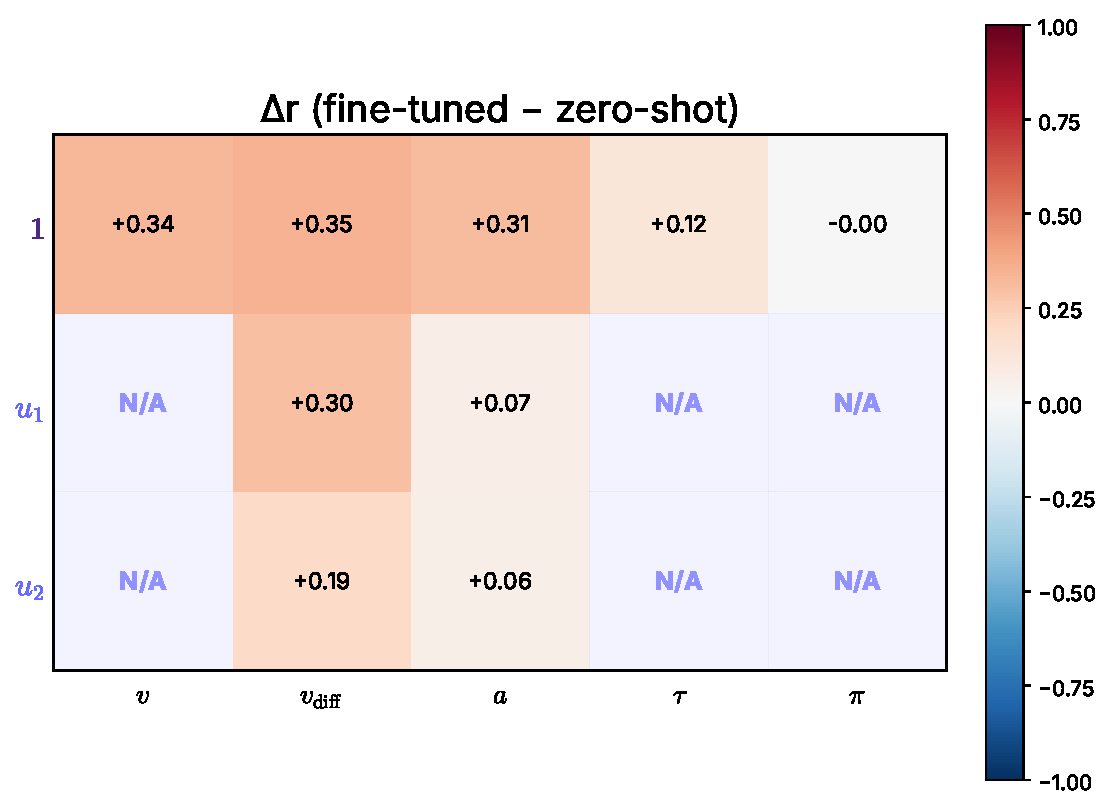
\includegraphics[width=\textwidth,height=0.18\textheight,keepaspectratio]{compare/lba/fixed_regressed_delta_r.pdf}
    \caption{}
  \end{subfigure}\\[0.5ex]
  \begin{subfigure}{\textwidth}\centering
    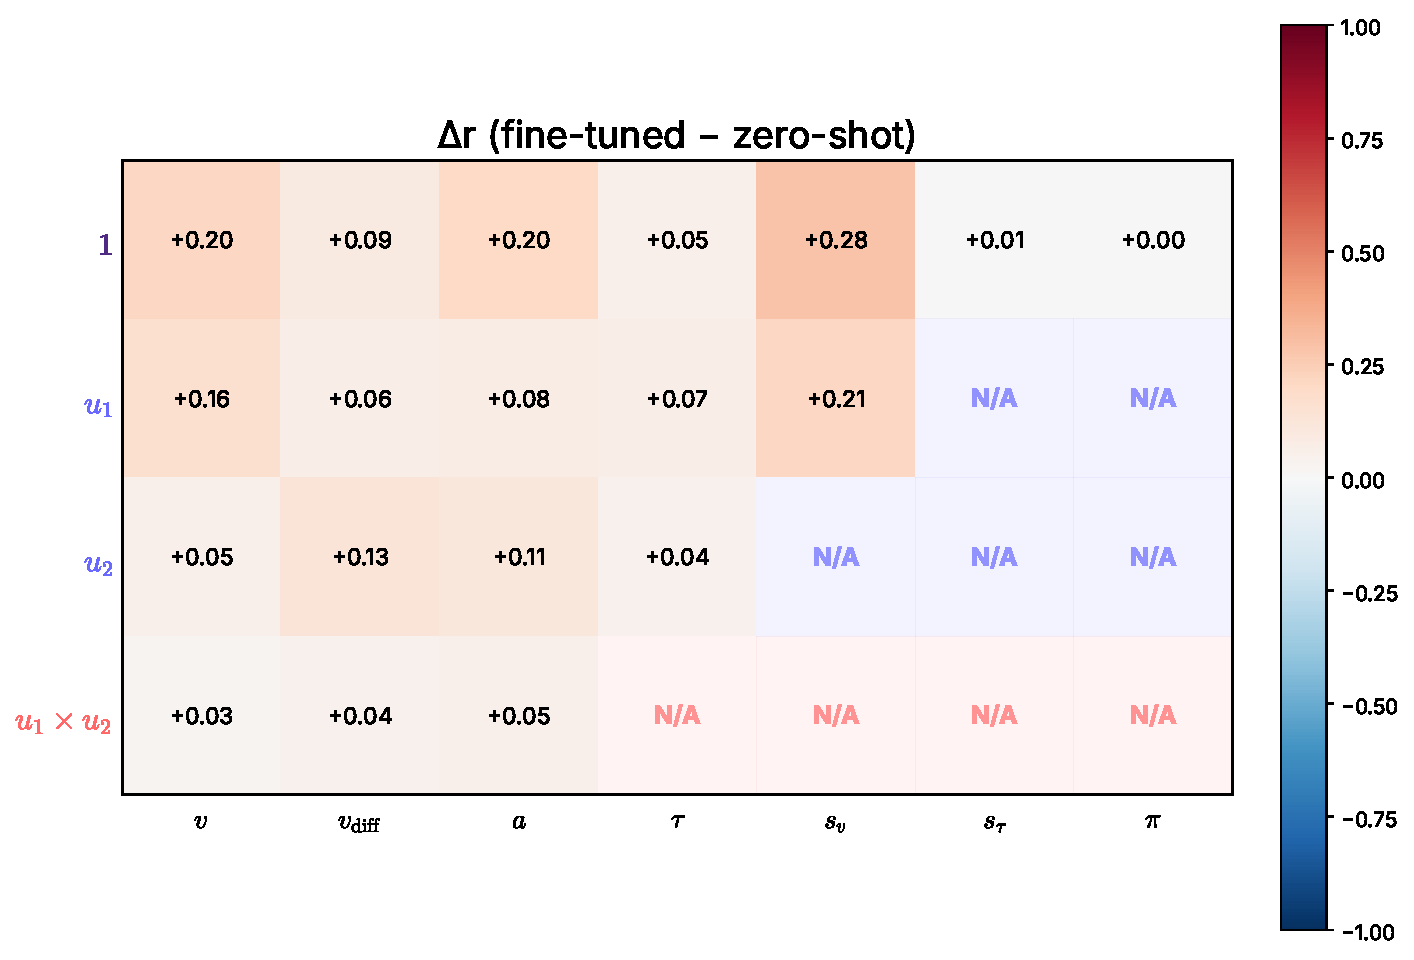
\includegraphics[width=\textwidth,height=0.18\textheight,keepaspectratio]{compare/lba/interaction_delta_r.pdf}
    \caption{}
  \end{subfigure}
  \caption{\textbf{Change in parameter recovery with fine-tuning: LBA.} $\Delta r = r_{\text{fine-tuned}} - r_{\text{zero-shot}}$ per coefficient for the five bench5 designs, (a) intercept-only, (b) fixed, (c) regressed, (d) fixed + regressed, (e) interaction, where $r$ is the Pearson correlation between the posterior mean (200 draws) and the ground truth across the 200 test datasets; both networks are scored on identical datasets. Red marks better recovery after fine-tuning, blue worse, on a common scale from $-1$ to $1$; each cell is annotated with its $\Delta r$. Rows are the coefficients of the design and columns the parameters, including $\pi$; N/A marks coefficients the design does not contain. Values are point estimates; no uncertainty is shown. Figures~\ref{fig:app3-delta-r-ddm}--\ref{fig:app3-delta-r-cdm} show the same maps for DDM, RDM and CDM, where $\Delta r$ compares the fine-tuned network with the original one and so measures forgetting.}
  \label{fig:app3-delta-r-lba}
\end{figure}

\begin{figure}[p]
  \centering
  \begin{subfigure}{\textwidth}\centering
    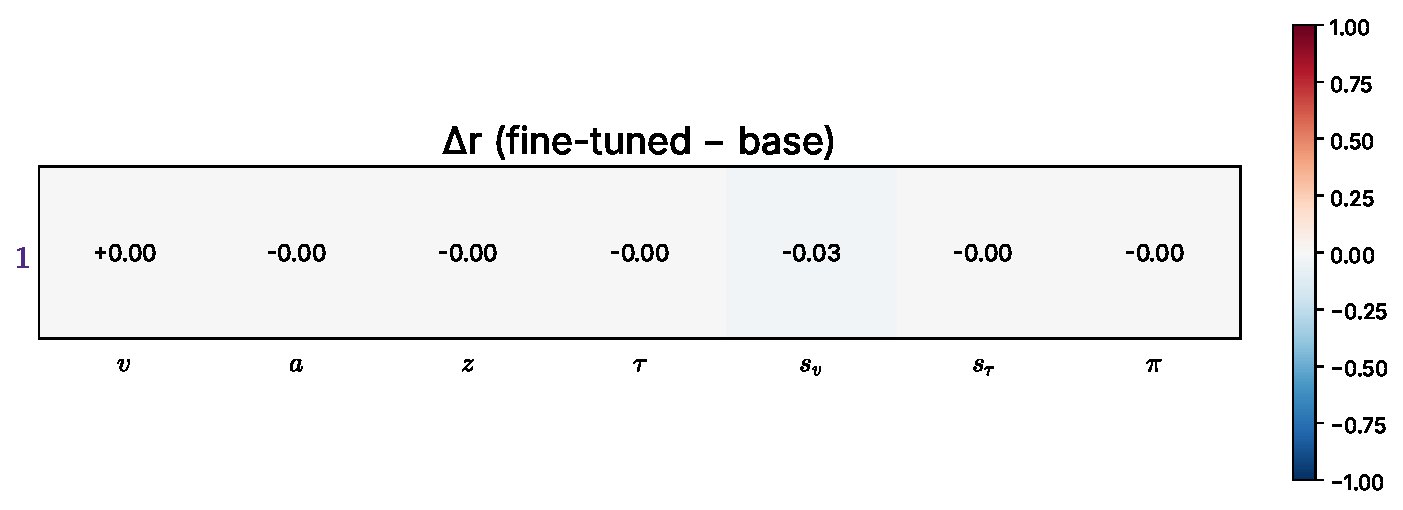
\includegraphics[width=\textwidth,height=0.18\textheight,keepaspectratio]{compare/ddm/intercept_only_forgetting_delta_r.pdf}
    \caption{}
  \end{subfigure}\\[0.5ex]
  \begin{subfigure}{\textwidth}\centering
    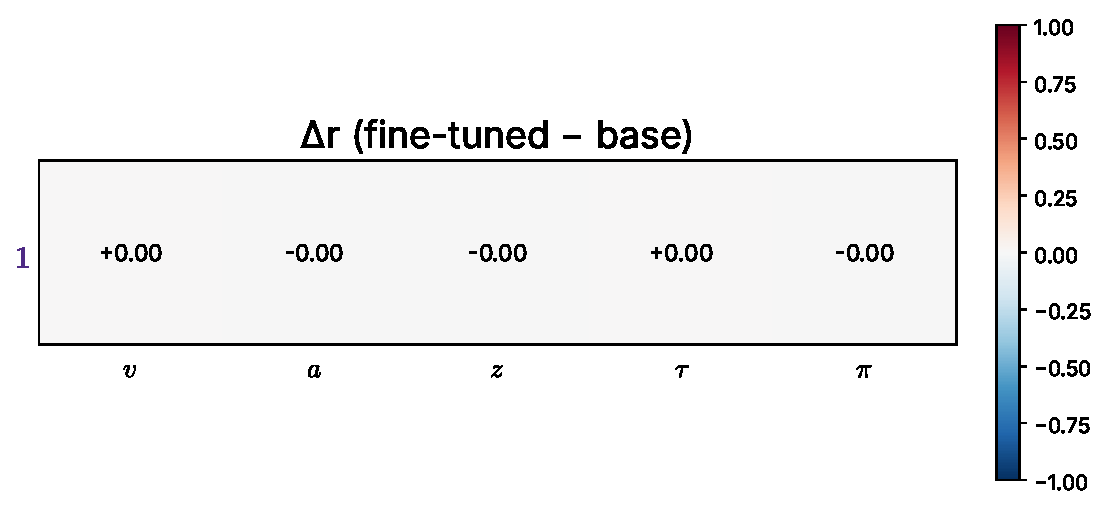
\includegraphics[width=\textwidth,height=0.18\textheight,keepaspectratio]{compare/ddm/fixed_forgetting_delta_r.pdf}
    \caption{}
  \end{subfigure}\\[0.5ex]
  \begin{subfigure}{\textwidth}\centering
    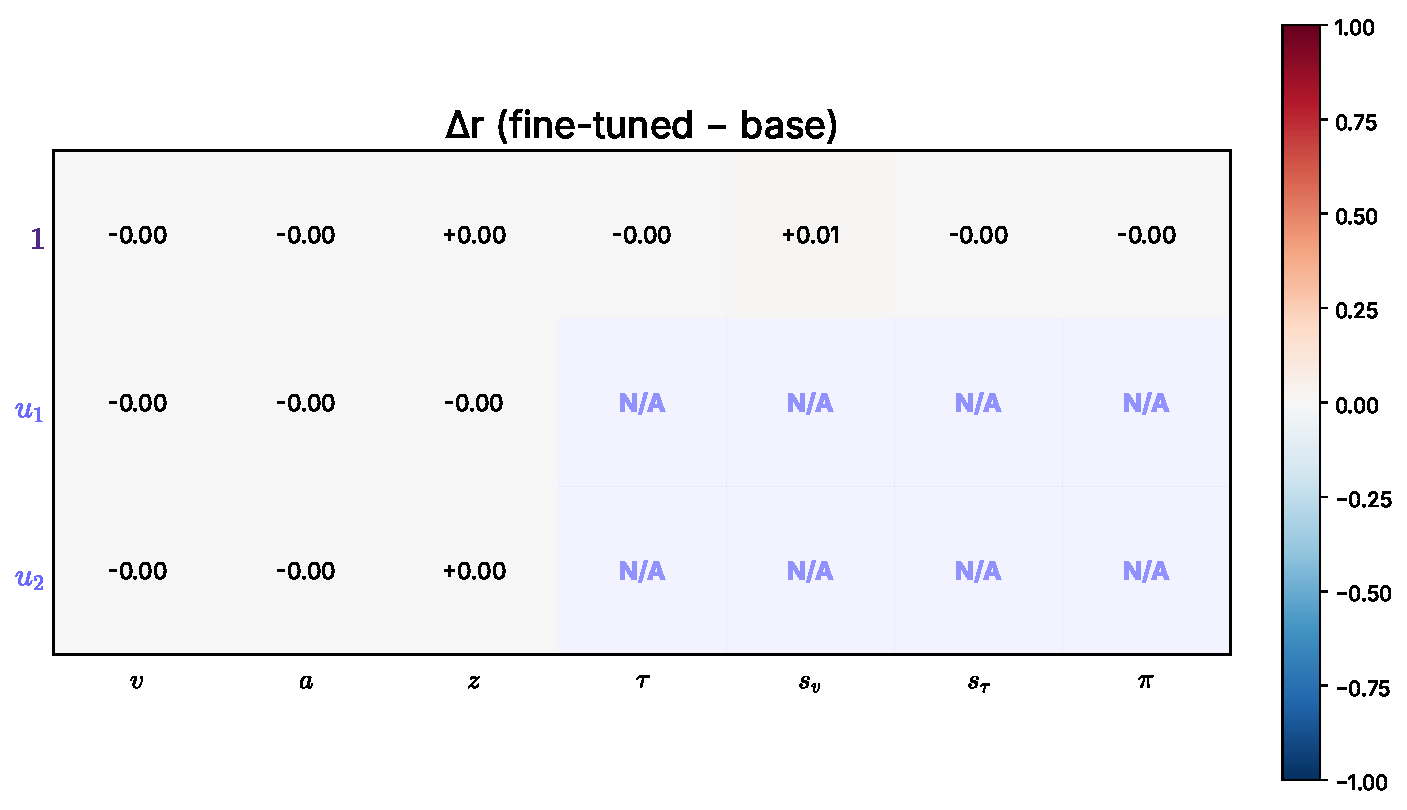
\includegraphics[width=\textwidth,height=0.18\textheight,keepaspectratio]{compare/ddm/regressed_forgetting_delta_r.pdf}
    \caption{}
  \end{subfigure}\\[0.5ex]
  \begin{subfigure}{\textwidth}\centering
    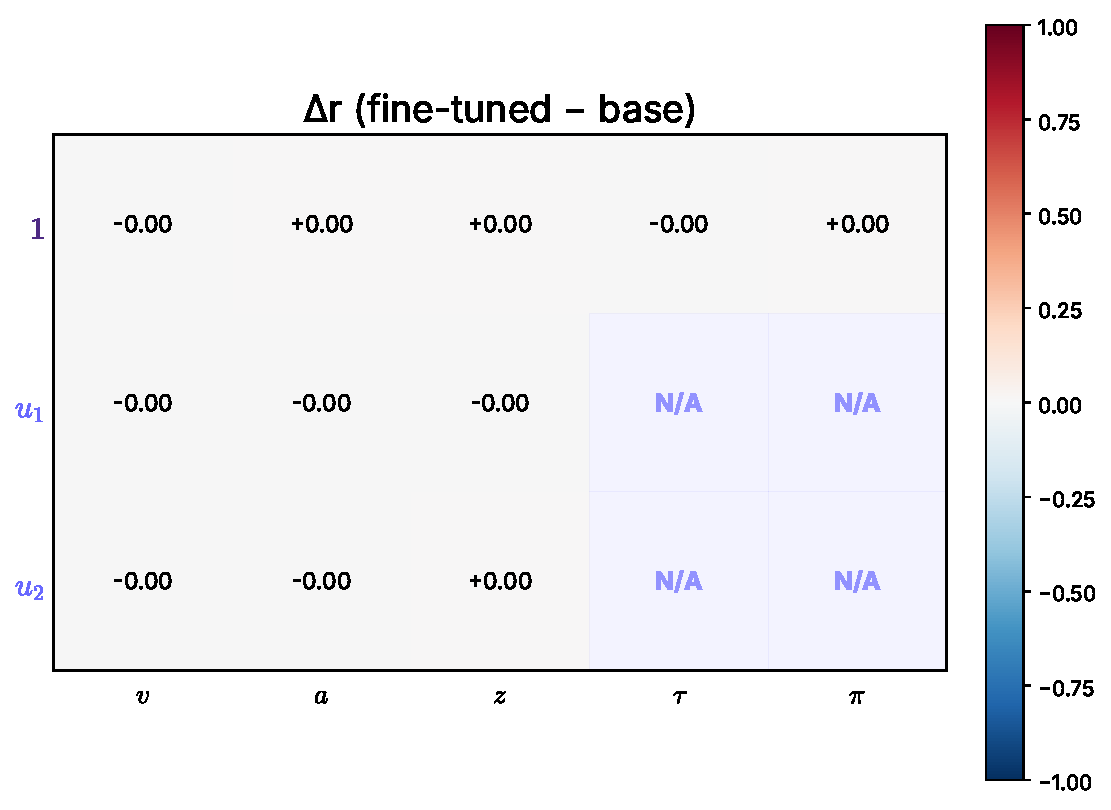
\includegraphics[width=\textwidth,height=0.18\textheight,keepaspectratio]{compare/ddm/fixed_regressed_forgetting_delta_r.pdf}
    \caption{}
  \end{subfigure}\\[0.5ex]
  \begin{subfigure}{\textwidth}\centering
    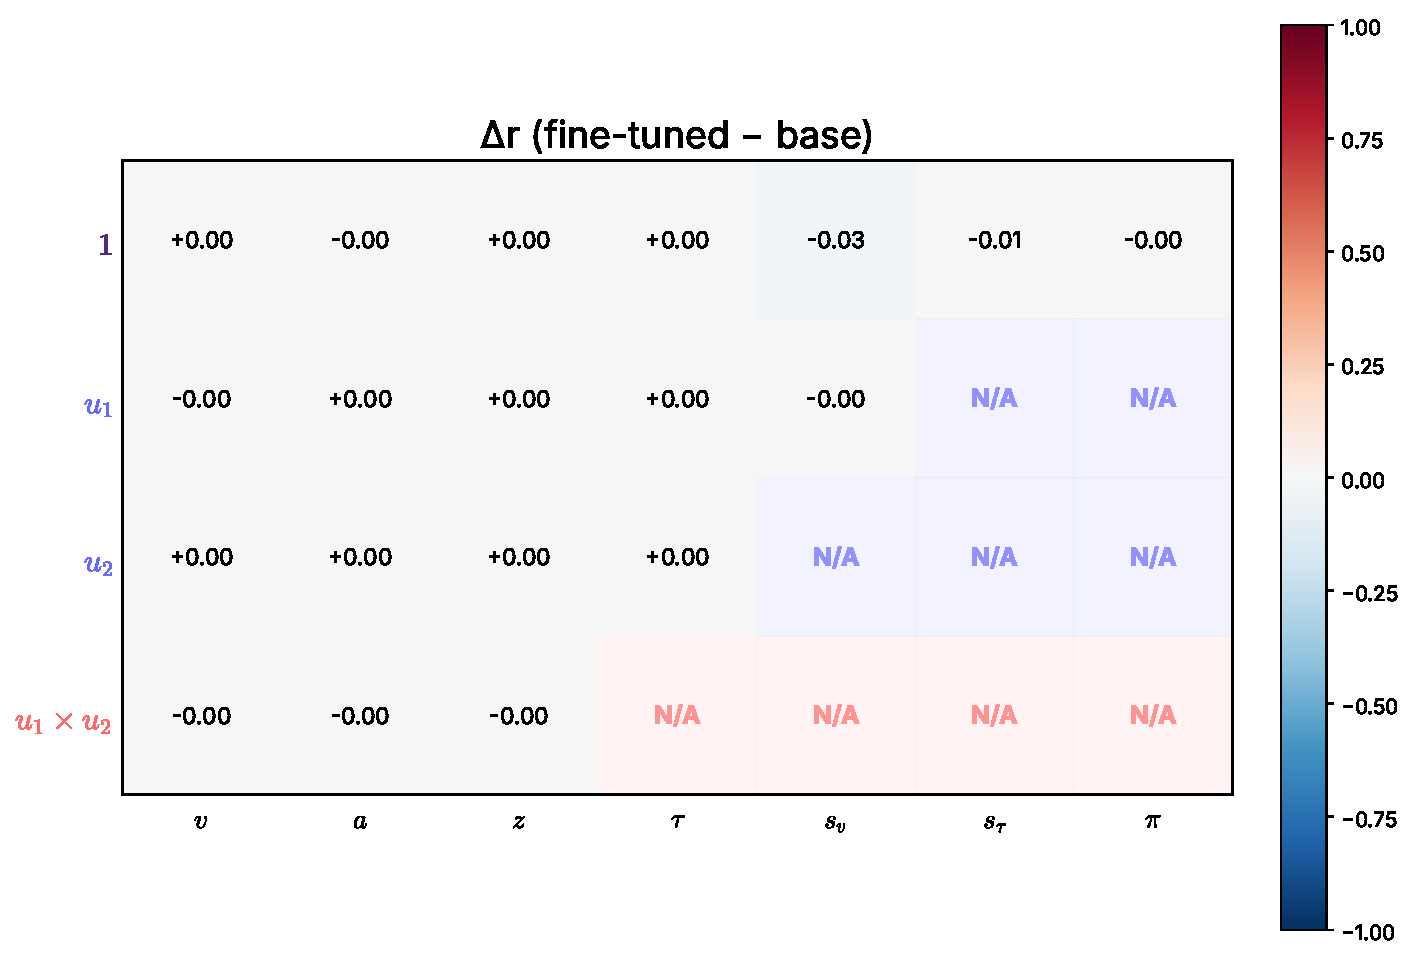
\includegraphics[width=\textwidth,height=0.18\textheight,keepaspectratio]{compare/ddm/interaction_forgetting_delta_r.pdf}
    \caption{}
  \end{subfigure}
  \caption{\textbf{Forgetting in parameter recovery: DDM.} $\Delta r = r_{\text{fine-tuned}} - r_{\text{original}}$ (the original network is labelled ``base'' in the panels) for (a) intercept-only, (b) fixed, (c) regressed, (d) fixed + regressed, (e) interaction, on the identical bench5 datasets; encoding as in Figure~\ref{fig:app3-delta-r-lba}.}
  \label{fig:app3-delta-r-ddm}
\end{figure}

\begin{figure}[p]
  \centering
  \begin{subfigure}{\textwidth}\centering
    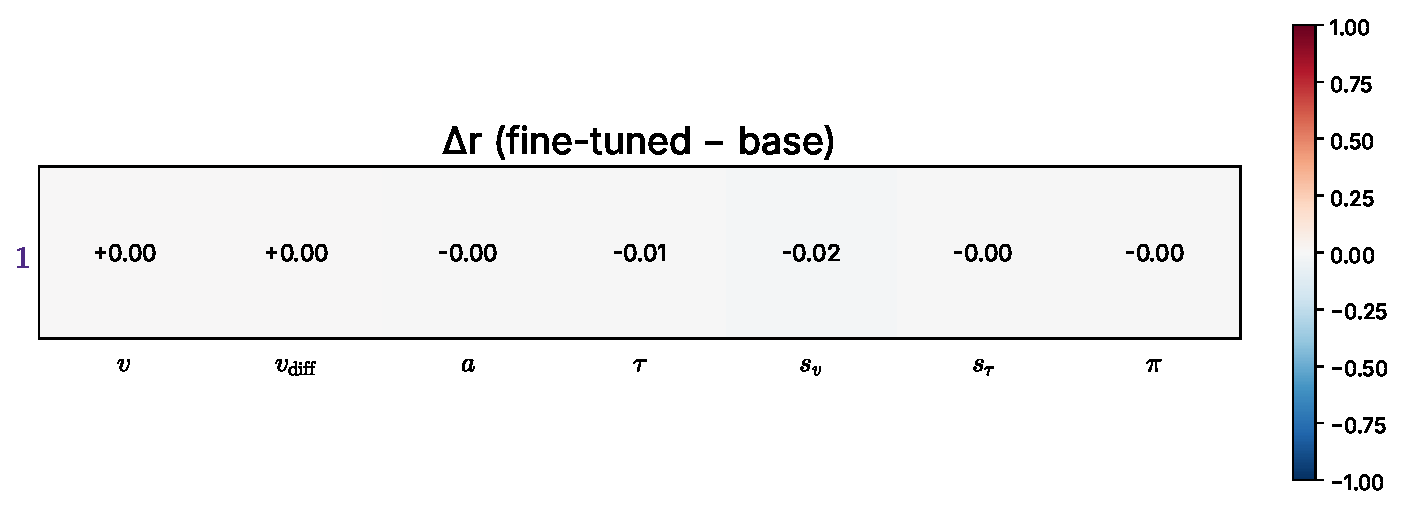
\includegraphics[width=\textwidth,height=0.18\textheight,keepaspectratio]{compare/rdm/intercept_only_forgetting_delta_r.pdf}
    \caption{}
  \end{subfigure}\\[0.5ex]
  \begin{subfigure}{\textwidth}\centering
    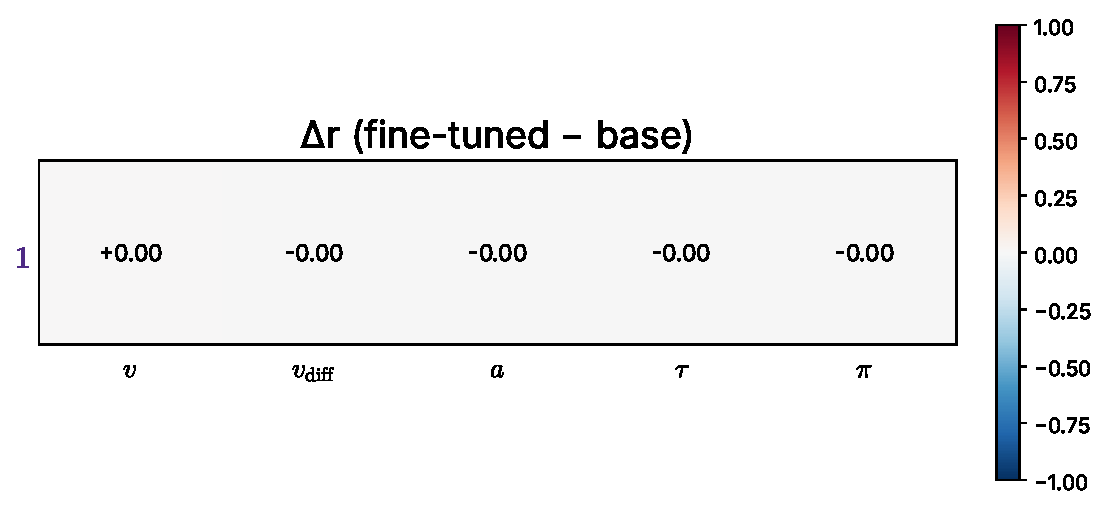
\includegraphics[width=\textwidth,height=0.18\textheight,keepaspectratio]{compare/rdm/fixed_forgetting_delta_r.pdf}
    \caption{}
  \end{subfigure}\\[0.5ex]
  \begin{subfigure}{\textwidth}\centering
    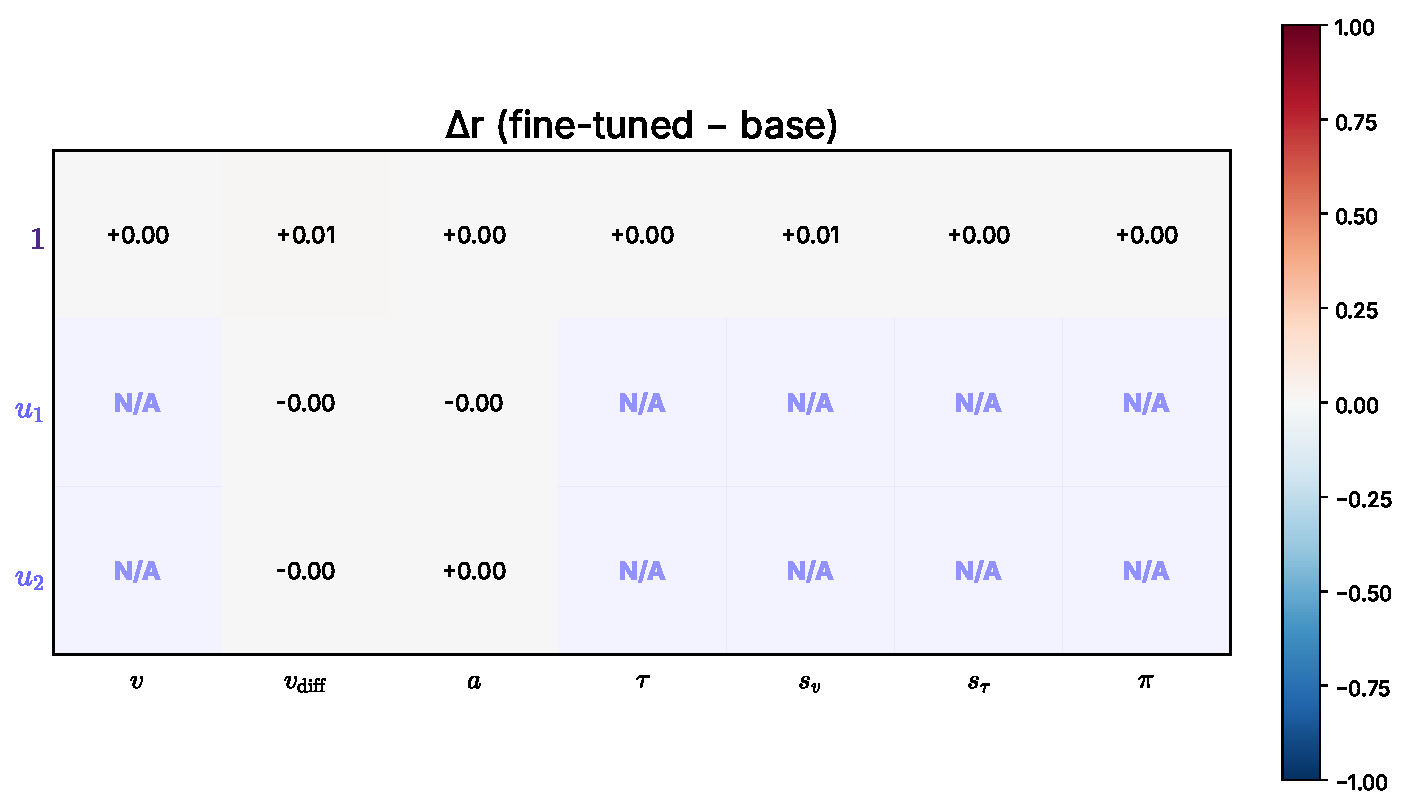
\includegraphics[width=\textwidth,height=0.18\textheight,keepaspectratio]{compare/rdm/regressed_forgetting_delta_r.pdf}
    \caption{}
  \end{subfigure}\\[0.5ex]
  \begin{subfigure}{\textwidth}\centering
    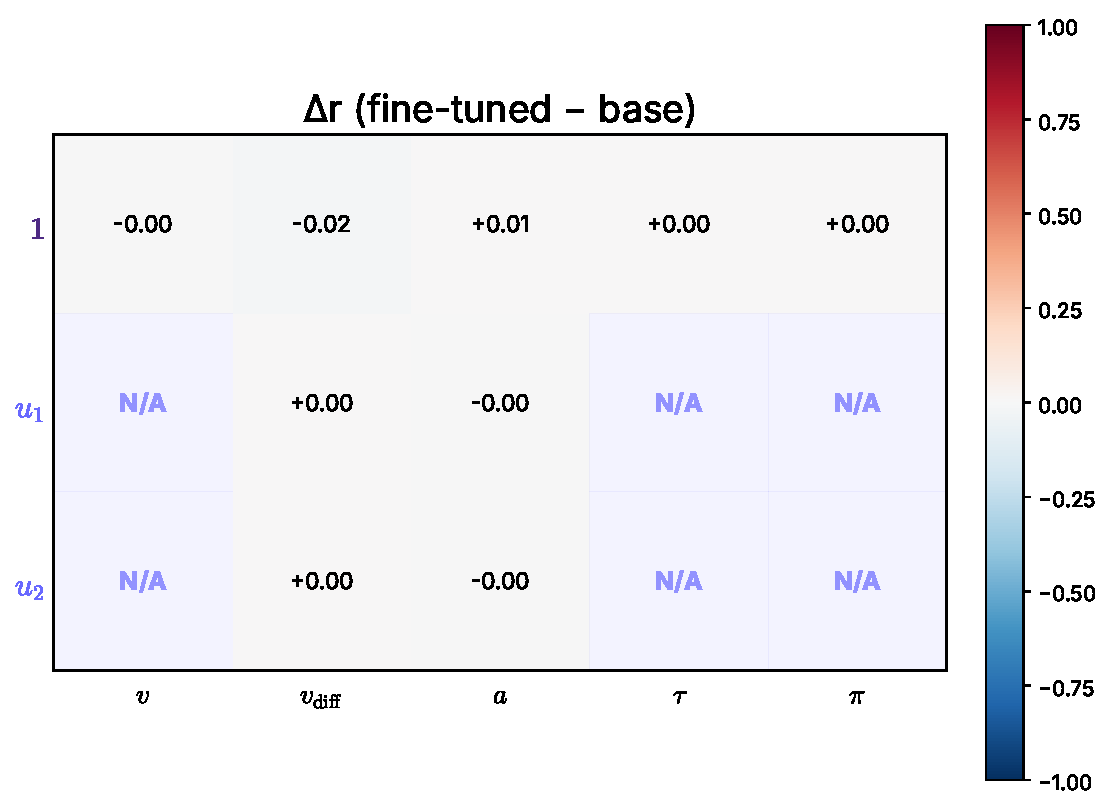
\includegraphics[width=\textwidth,height=0.18\textheight,keepaspectratio]{compare/rdm/fixed_regressed_forgetting_delta_r.pdf}
    \caption{}
  \end{subfigure}\\[0.5ex]
  \begin{subfigure}{\textwidth}\centering
    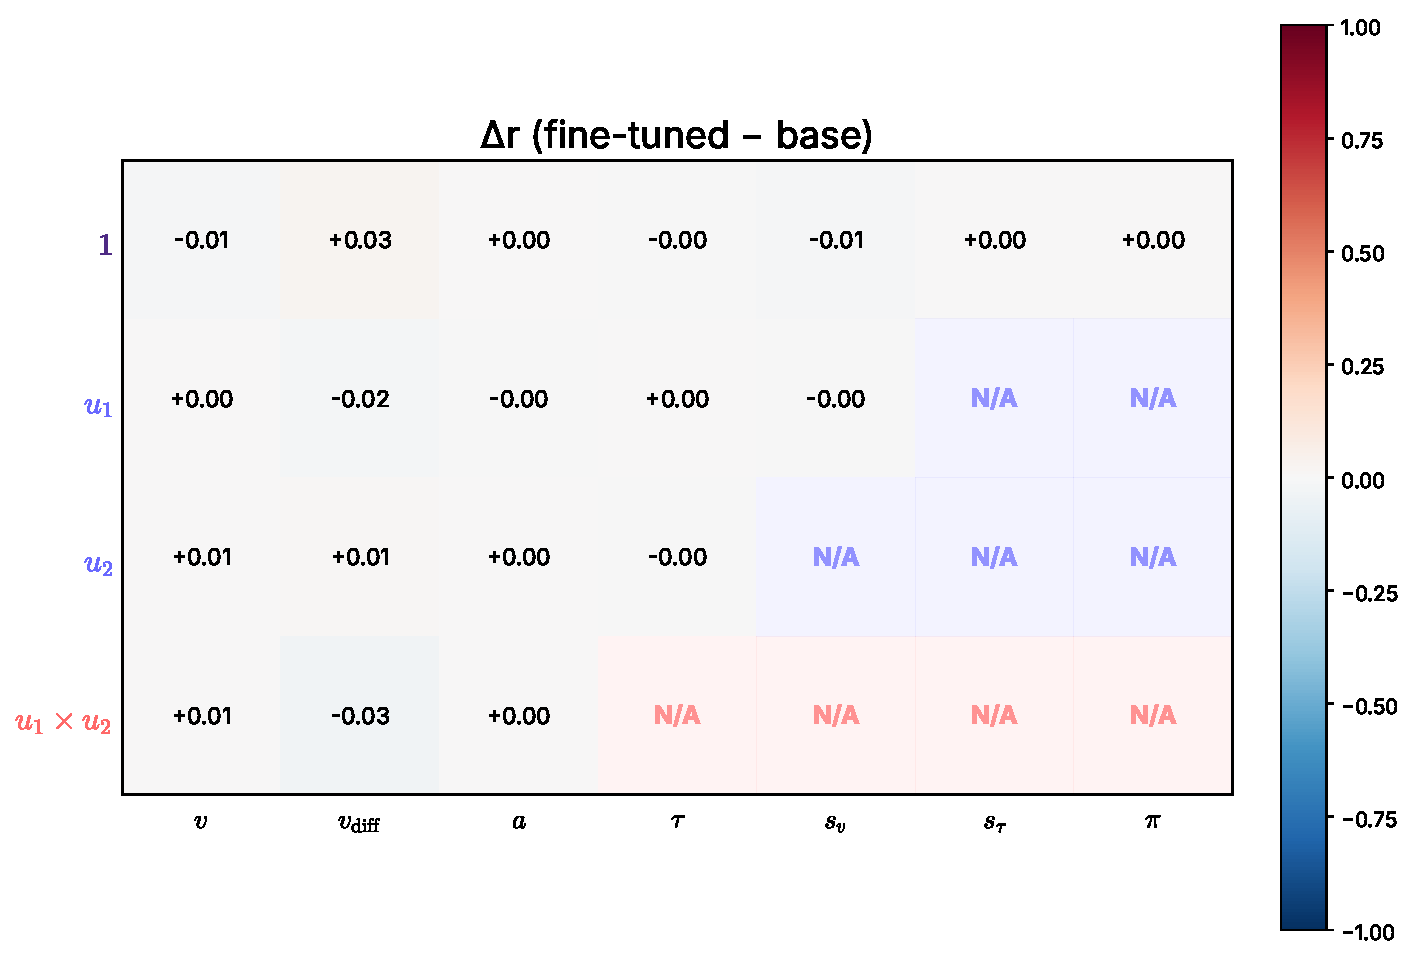
\includegraphics[width=\textwidth,height=0.18\textheight,keepaspectratio]{compare/rdm/interaction_forgetting_delta_r.pdf}
    \caption{}
  \end{subfigure}
  \caption{\textbf{Forgetting in parameter recovery: RDM.} $\Delta r = r_{\text{fine-tuned}} - r_{\text{original}}$ (the original network is labelled ``base'' in the panels) for (a) intercept-only, (b) fixed, (c) regressed, (d) fixed + regressed, (e) interaction, on the identical bench5 datasets; encoding as in Figure~\ref{fig:app3-delta-r-lba}.}
  \label{fig:app3-delta-r-rdm}
\end{figure}

\begin{figure}[p]
  \centering
  \begin{subfigure}{\textwidth}\centering
    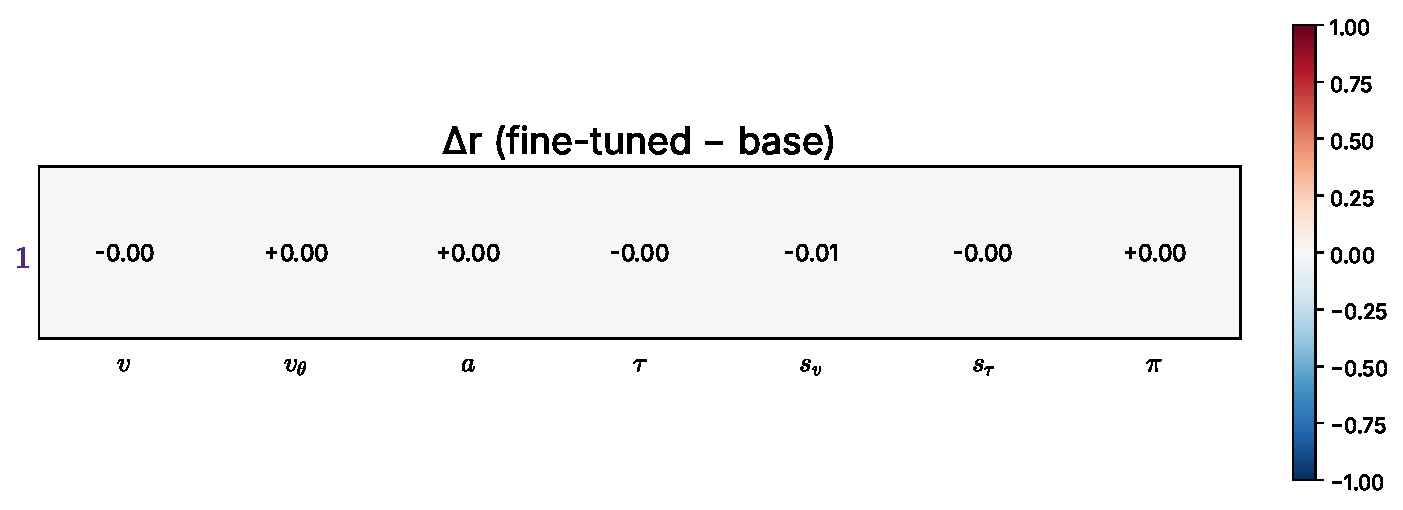
\includegraphics[width=\textwidth,height=0.18\textheight,keepaspectratio]{compare/cdm/intercept_only_forgetting_delta_r.pdf}
    \caption{}
  \end{subfigure}\\[0.5ex]
  \begin{subfigure}{\textwidth}\centering
    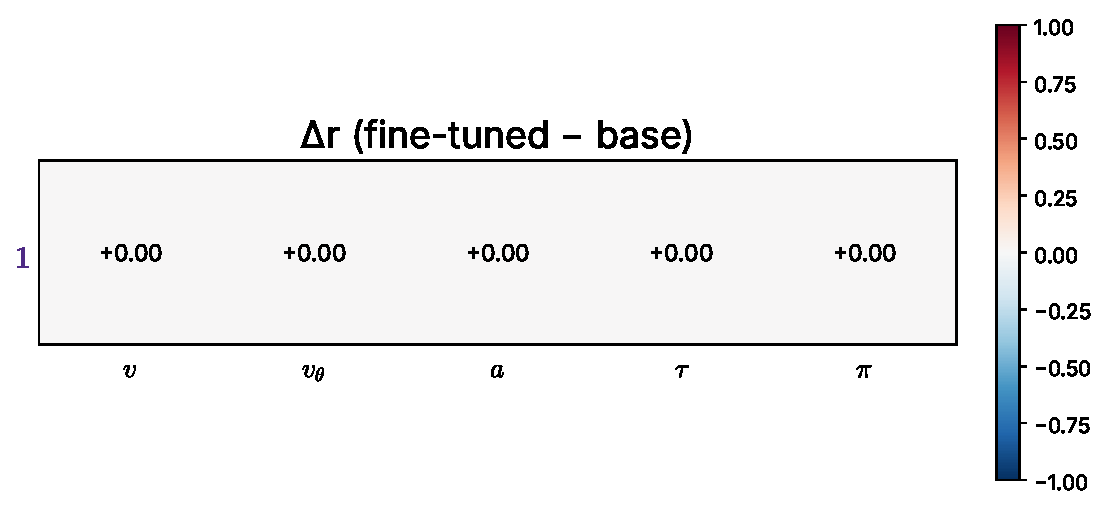
\includegraphics[width=\textwidth,height=0.18\textheight,keepaspectratio]{compare/cdm/fixed_forgetting_delta_r.pdf}
    \caption{}
  \end{subfigure}\\[0.5ex]
  \begin{subfigure}{\textwidth}\centering
    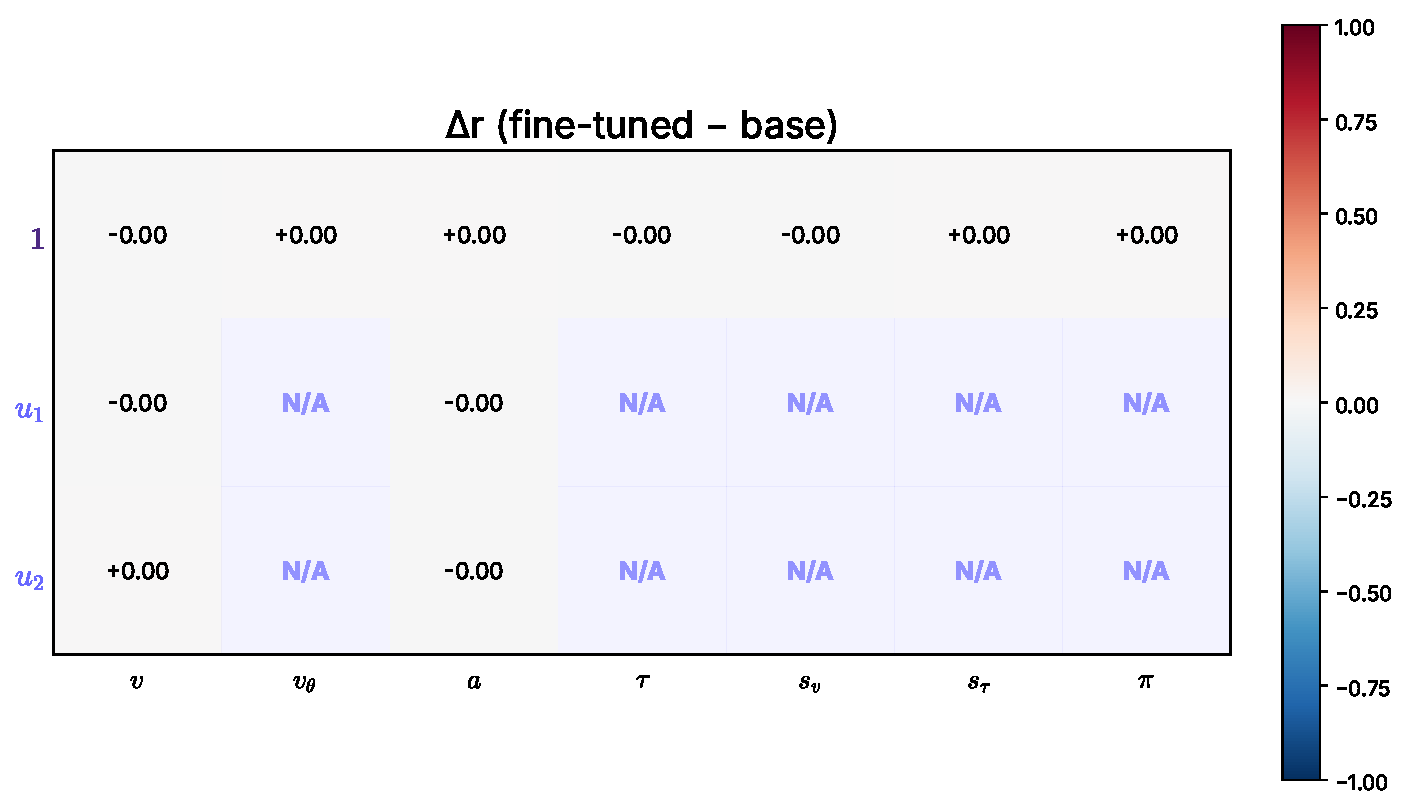
\includegraphics[width=\textwidth,height=0.18\textheight,keepaspectratio]{compare/cdm/regressed_forgetting_delta_r.pdf}
    \caption{}
  \end{subfigure}\\[0.5ex]
  \begin{subfigure}{\textwidth}\centering
    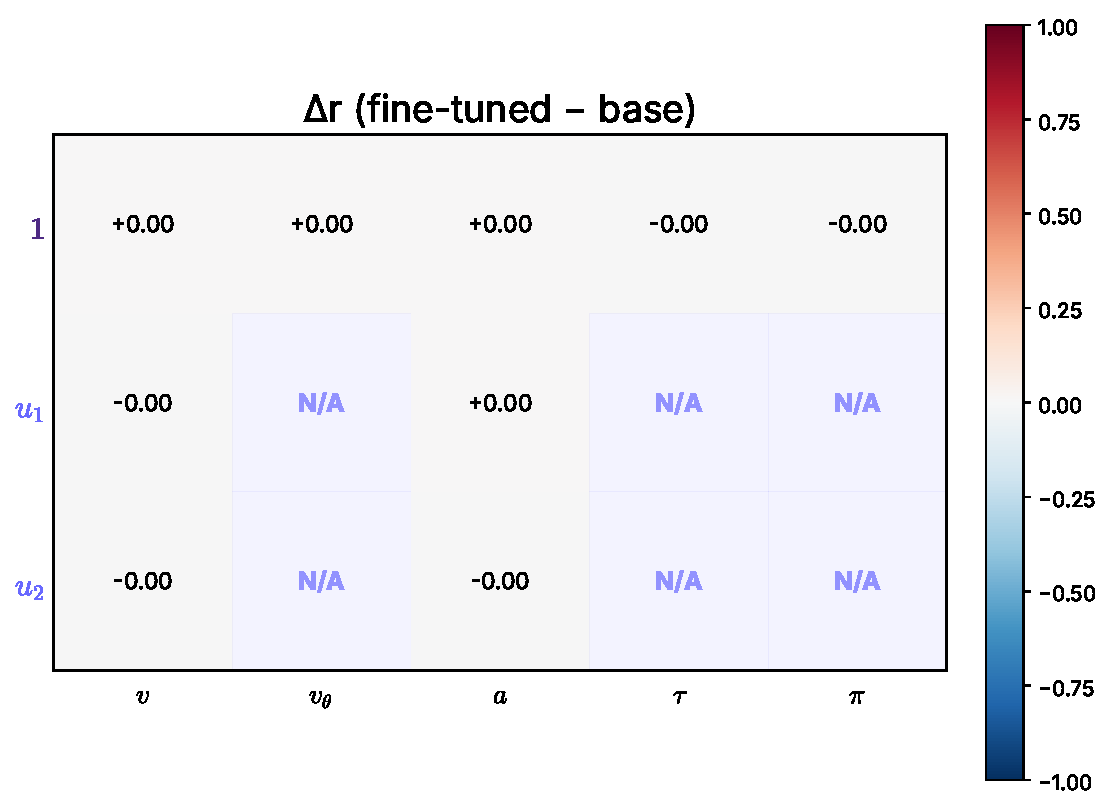
\includegraphics[width=\textwidth,height=0.18\textheight,keepaspectratio]{compare/cdm/fixed_regressed_forgetting_delta_r.pdf}
    \caption{}
  \end{subfigure}\\[0.5ex]
  \begin{subfigure}{\textwidth}\centering
    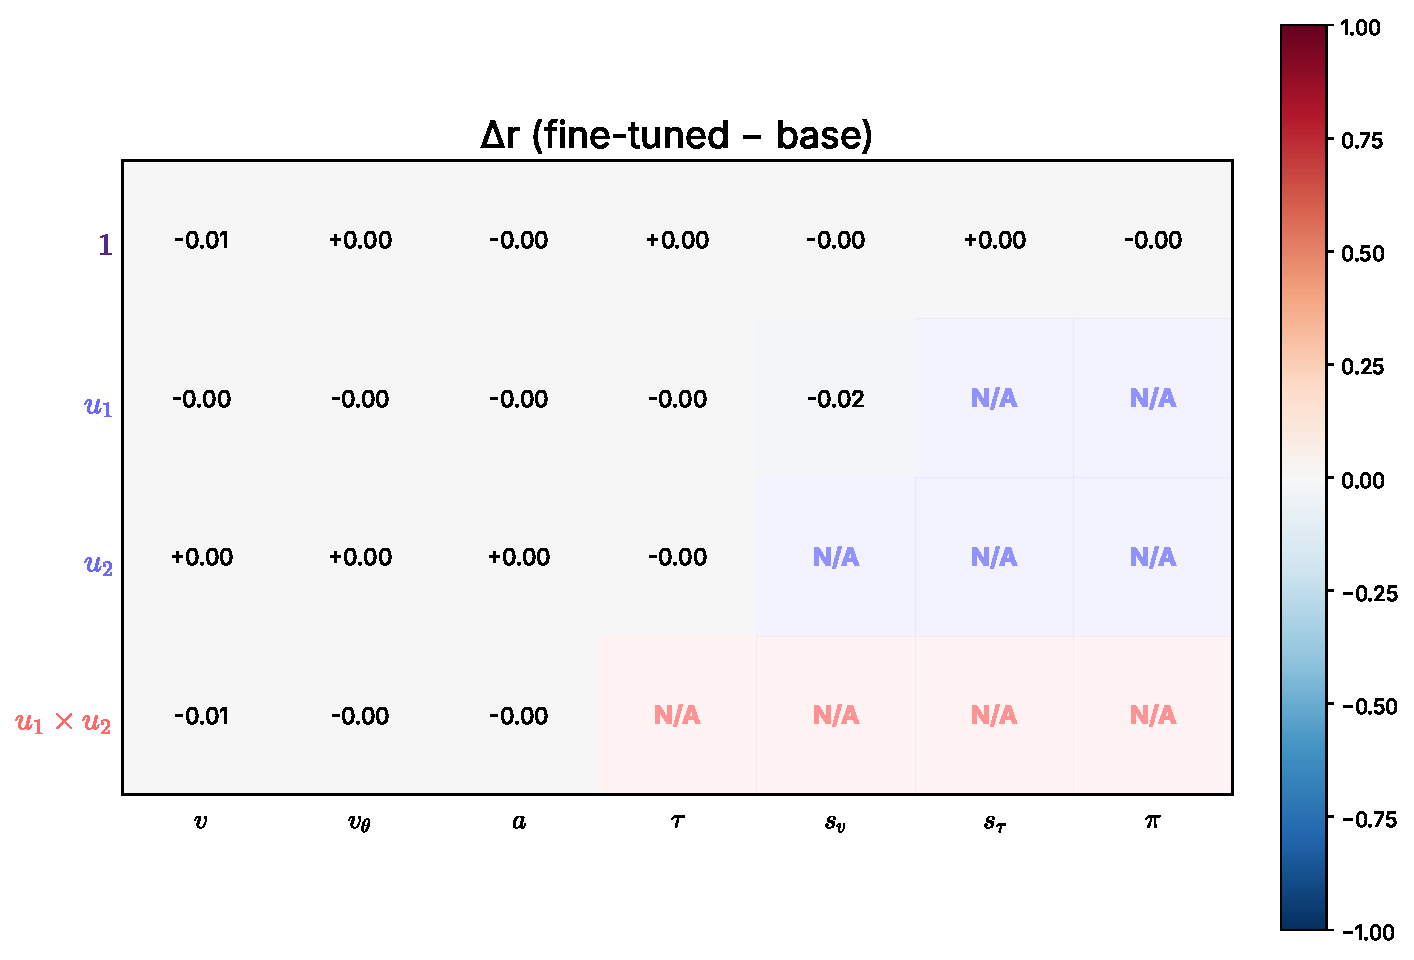
\includegraphics[width=\textwidth,height=0.18\textheight,keepaspectratio]{compare/cdm/interaction_forgetting_delta_r.pdf}
    \caption{}
  \end{subfigure}
  \caption{\textbf{Forgetting in parameter recovery: CDM.} $\Delta r = r_{\text{fine-tuned}} - r_{\text{original}}$ (the original network is labelled ``base'' in the panels) for (a) intercept-only, (b) fixed, (c) regressed, (d) fixed + regressed, (e) interaction, on the identical bench5 datasets; encoding as in Figure~\ref{fig:app3-delta-r-lba}.}
  \label{fig:app3-delta-r-cdm}
\end{figure}

% ── 4. change in metrics ──

\begin{figure}[p]
  \centering
  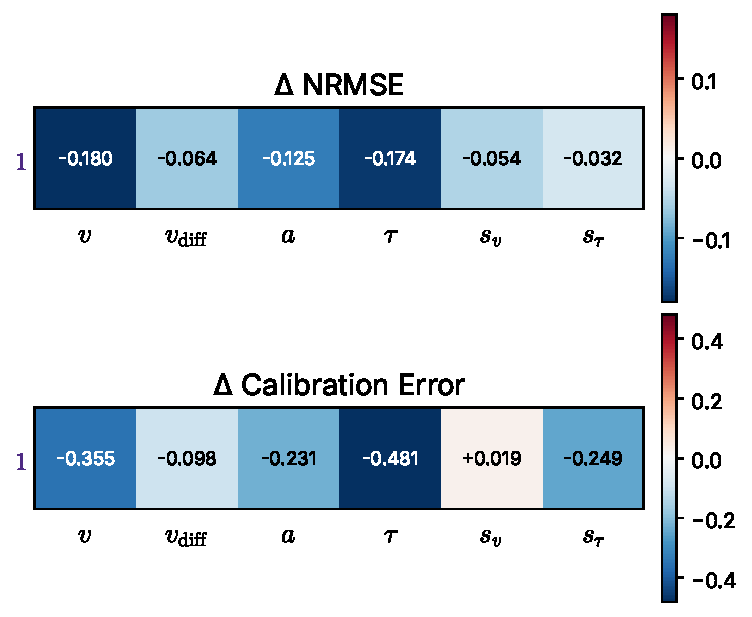
\includegraphics[width=\textwidth,height=0.45\textheight,keepaspectratio]{compare/delta_metrics_intercept_only.pdf}
  \caption{\textbf{Change in the LBA's summary metrics with fine-tuning, \emph{intercept-only} design.} Per-coefficient change in NRMSE (top) and calibration error (bottom), fine-tuned minus zero-shot, both networks scored on identical bench5 test datasets, with the metric definitions of the bottom panel of Figure~\ref{fig:app1-ddm-intercept-only-cf}. Negative values (blue) are improvements, positive values (red) deteriorations; each panel has its own colour scale. Columns are the parameters and rows the coefficients; N/A marks coefficients the design does not contain, and $\pi$ is not shown. Figures~\ref{fig:app3-delta-metrics-fixed}--\ref{fig:app3-delta-metrics-interaction} show the other designs.}
  \label{fig:app3-delta-metrics-intercept-only}
\end{figure}

\begin{figure}[p]
  \centering
  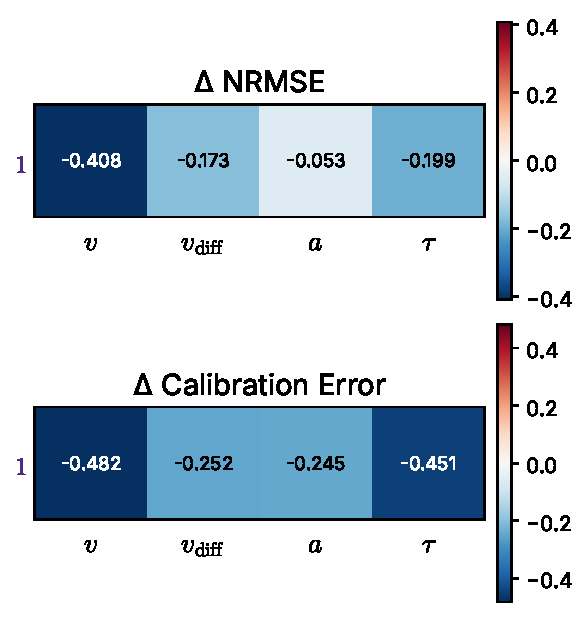
\includegraphics[width=\textwidth,height=0.45\textheight,keepaspectratio]{compare/delta_metrics_fixed.pdf}
  \caption{\textbf{Change in the LBA's summary metrics with fine-tuning, \emph{fixed} design.} As in Figure~\ref{fig:app3-delta-metrics-intercept-only}.}
  \label{fig:app3-delta-metrics-fixed}
\end{figure}

\begin{figure}[p]
  \centering
  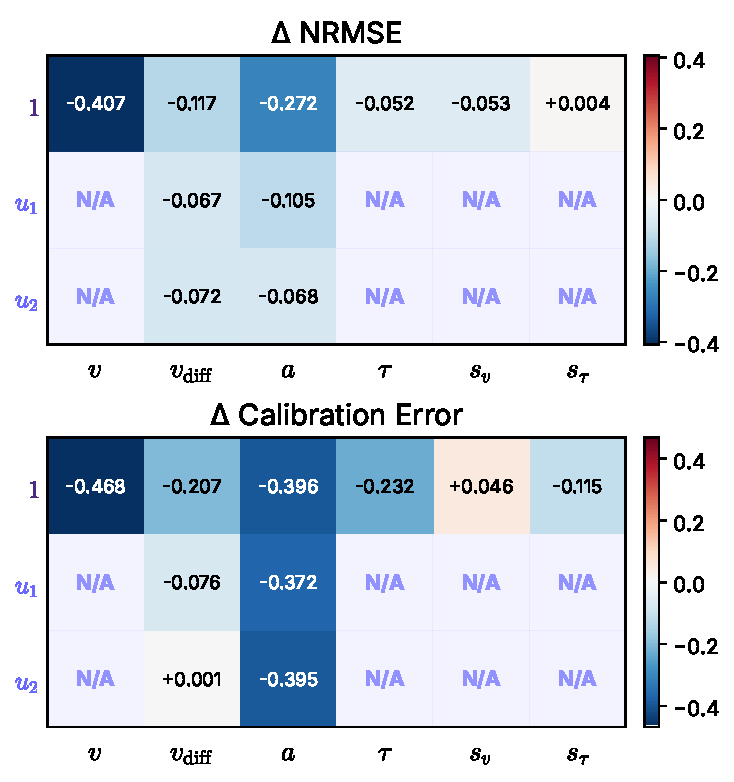
\includegraphics[width=\textwidth,height=0.45\textheight,keepaspectratio]{compare/delta_metrics_regressed.pdf}
  \caption{\textbf{Change in the LBA's summary metrics with fine-tuning, \emph{regressed} design.} As in Figure~\ref{fig:app3-delta-metrics-intercept-only}.}
  \label{fig:app3-delta-metrics-regressed}
\end{figure}

\begin{figure}[p]
  \centering
  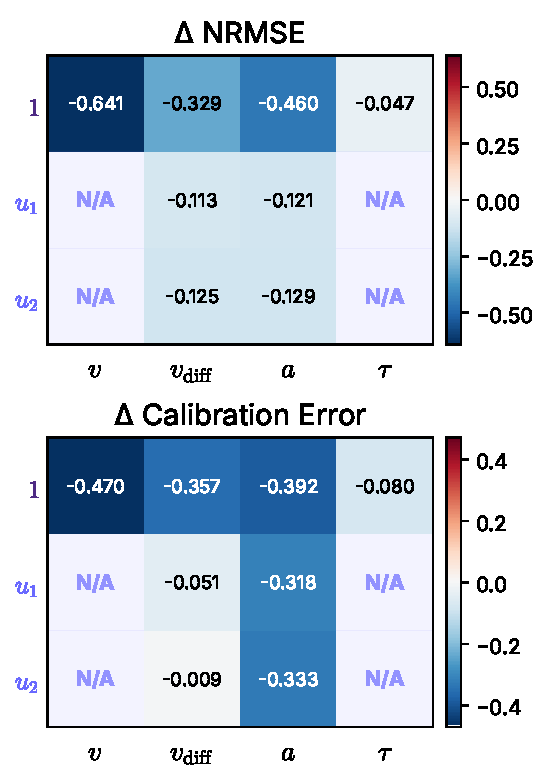
\includegraphics[width=\textwidth,height=0.45\textheight,keepaspectratio]{compare/delta_metrics_fixed_regressed.pdf}
  \caption{\textbf{Change in the LBA's summary metrics with fine-tuning, \emph{fixed + regressed} design.} As in Figure~\ref{fig:app3-delta-metrics-intercept-only}.}
  \label{fig:app3-delta-metrics-fixed-regressed}
\end{figure}

\begin{figure}[p]
  \centering
  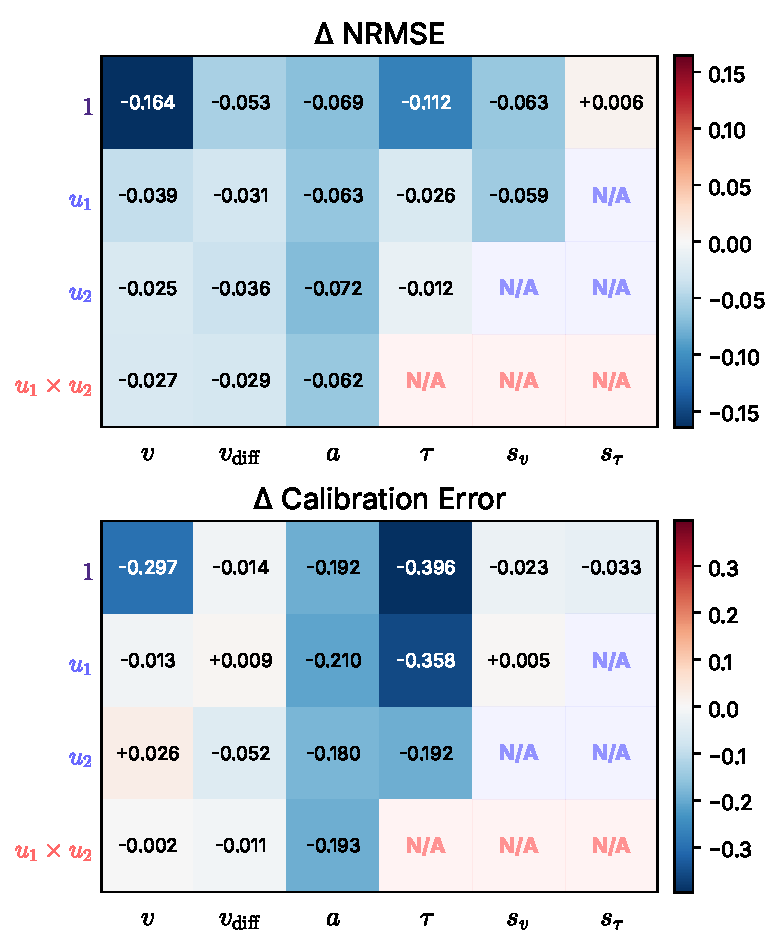
\includegraphics[width=\textwidth,height=0.45\textheight,keepaspectratio]{compare/delta_metrics_interaction.pdf}
  \caption{\textbf{Change in the LBA's summary metrics with fine-tuning, \emph{interaction} design.} As in Figure~\ref{fig:app3-delta-metrics-intercept-only}.}
  \label{fig:app3-delta-metrics-interaction}
\end{figure}

% ── 6. LBA amortization gap: baseline diagnostics ──

\begin{figure}[p]
  \centering
  \begin{subfigure}{\textwidth}\centering
    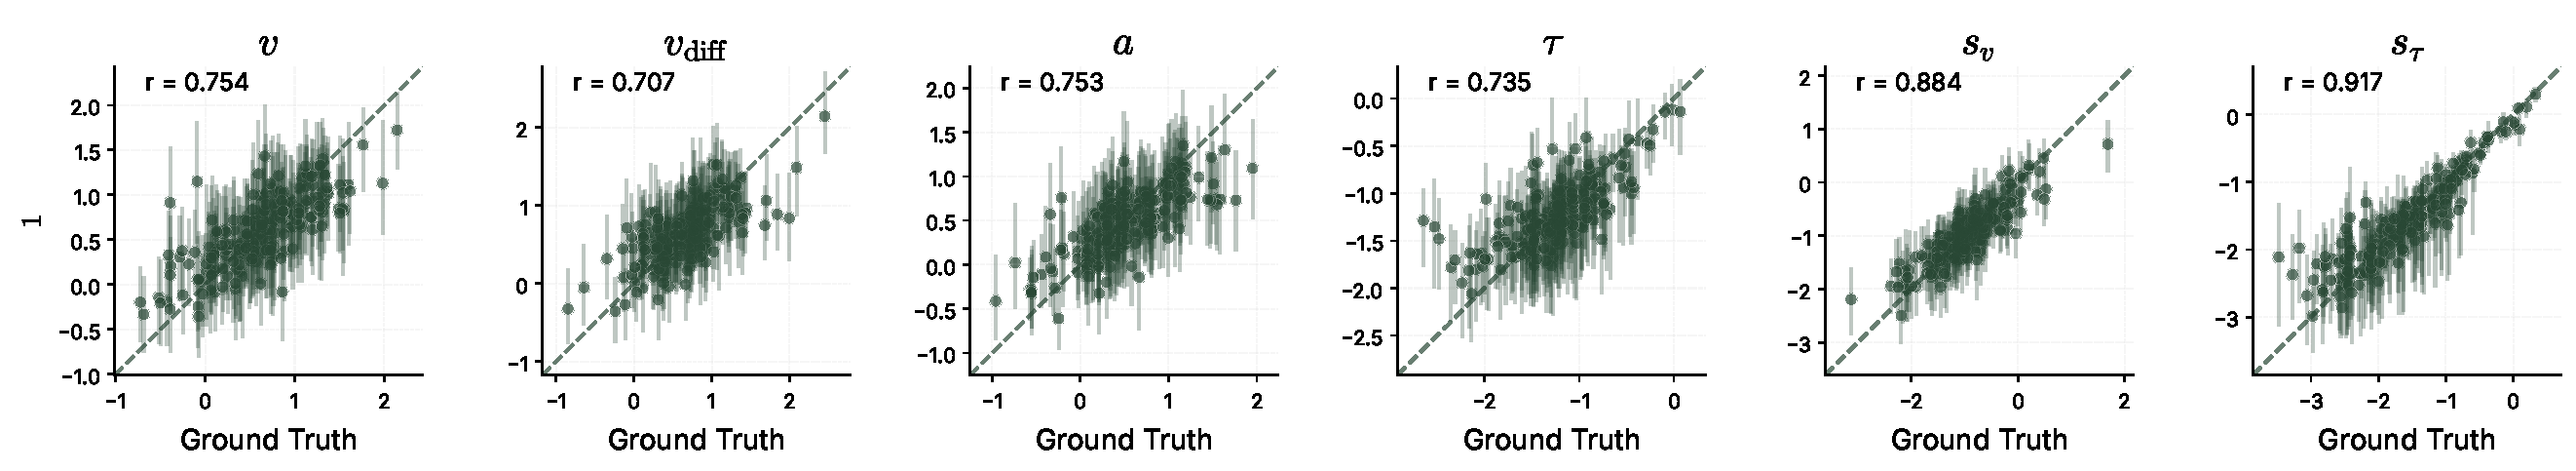
\includegraphics[width=\textwidth,height=0.3\textheight,keepaspectratio]{gap/intercept_only/bf_recovery.pdf}
    \caption{Recovery}
  \end{subfigure}\\[1ex]
  \begin{subfigure}{\textwidth}\centering
    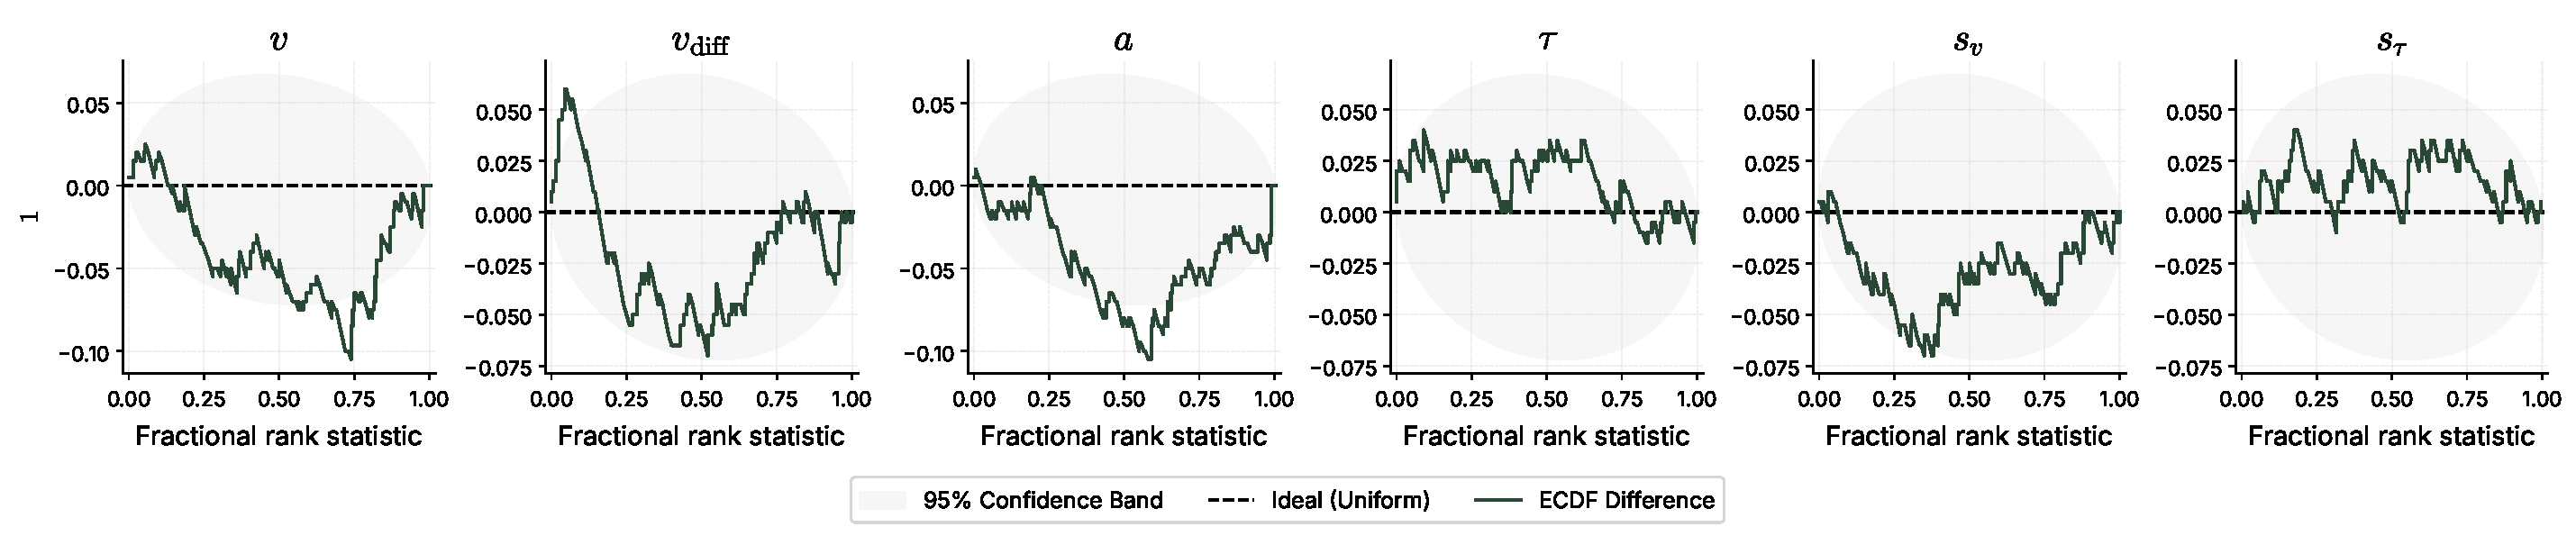
\includegraphics[width=\textwidth,height=0.3\textheight,keepaspectratio]{gap/intercept_only/bf_ecdf.pdf}
    \caption{Calibration (ECDF)}
  \end{subfigure}\\[1ex]
  \begin{subfigure}{\textwidth}\centering
    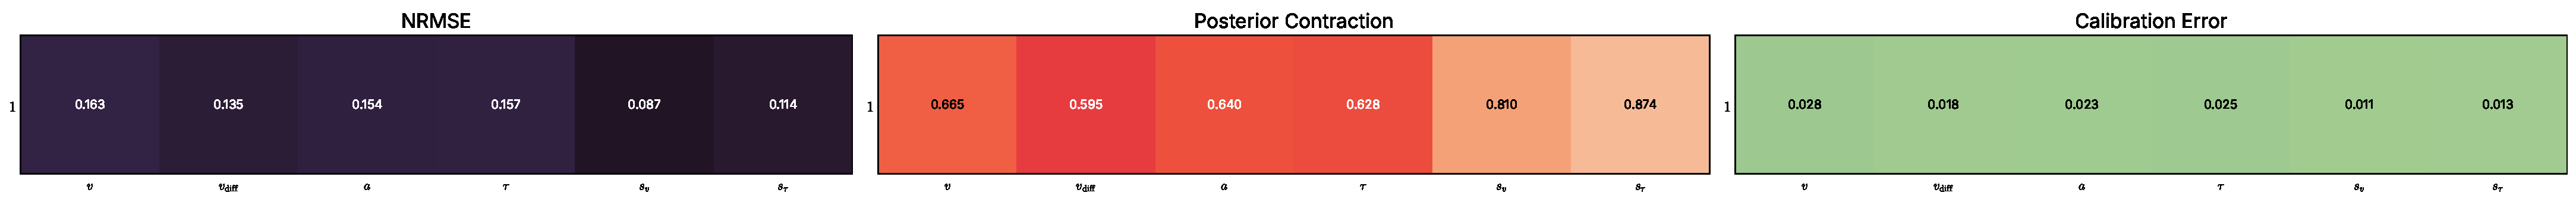
\includegraphics[width=\textwidth]{gap/intercept_only/bf_metrics.pdf}
    \caption{Metrics}
  \end{subfigure}
  \caption{\textbf{LBA amortization gap: BayesFlow baseline, \emph{intercept-only} design.} (a) Recovery, (b) calibration and (c) summary metrics of the case-specific BayesFlow baseline, trained for this LBA design alone (1000 epochs $\times$ 100 steps $\times$ batch 128, i.e.\ 12.8M simulated data sets, the per-case budget of the DDM/RDM/CDM baselines), on the same 200 bench5 LBA test datasets as the fine-tuned network (Figure~\ref{fig:app3-finetuned-lba-intercept-only}); encoding as in Figure~\ref{fig:app1-ddm-intercept-only-cf}. Every estimated parameter enters as an intercept only (6 coefficients shown). Figures~\ref{fig:app3-gap-lba-fixed}--\ref{fig:app3-gap-lba-interaction} show the other designs; Table~\ref{tab:app3-lba-gap-c2st} compares the two networks' posteriors.}
  \label{fig:app3-gap-lba-intercept-only}
\end{figure}

\begin{figure}[p]
  \centering
  \begin{subfigure}{\textwidth}\centering
    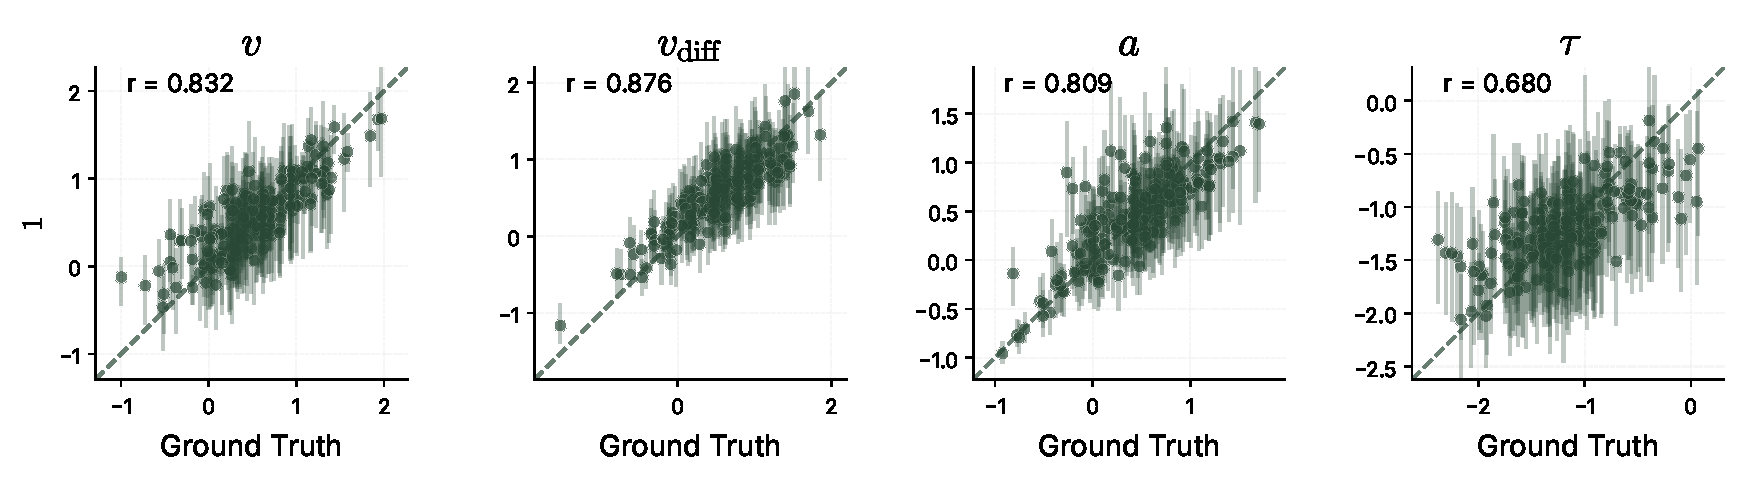
\includegraphics[width=\textwidth,height=0.3\textheight,keepaspectratio]{gap/fixed/bf_recovery.pdf}
    \caption{Recovery}
  \end{subfigure}\\[1ex]
  \begin{subfigure}{\textwidth}\centering
    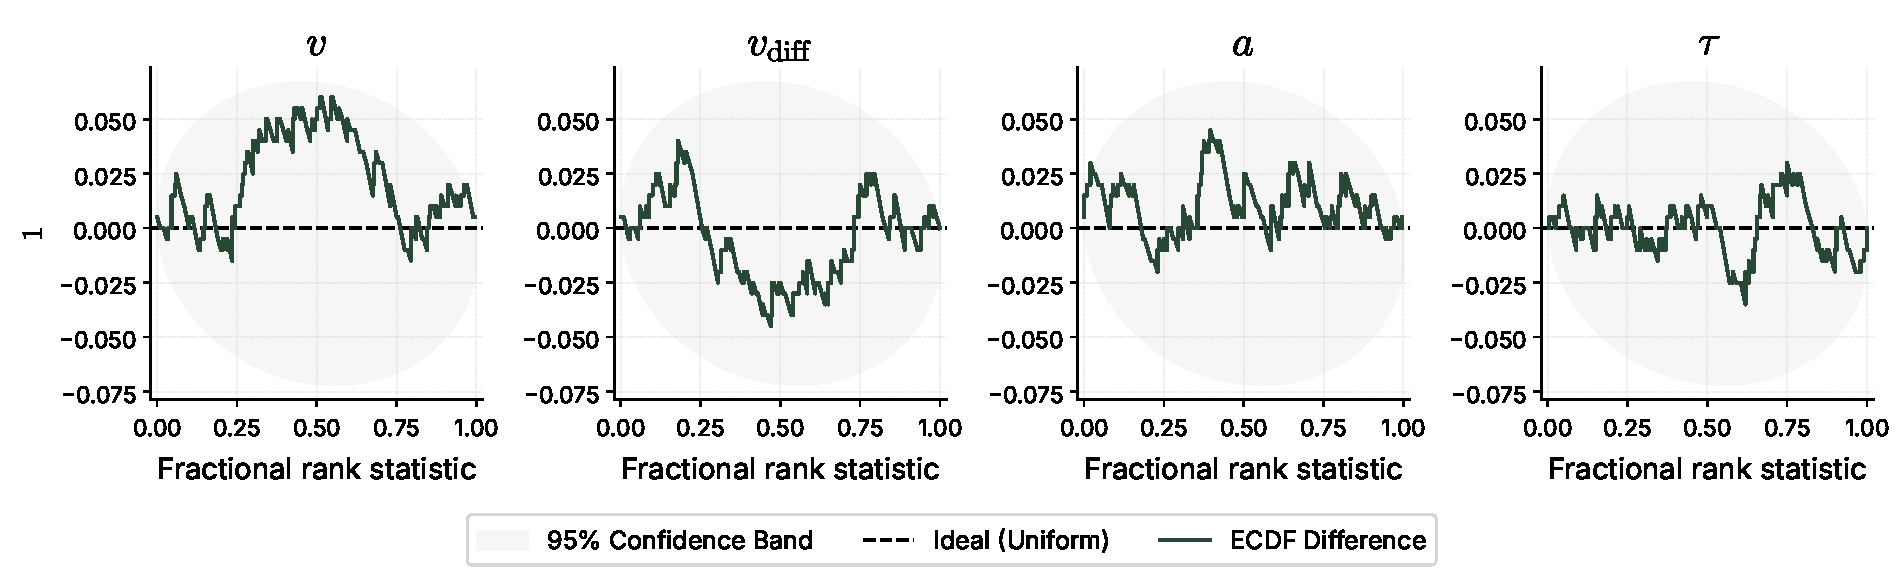
\includegraphics[width=\textwidth,height=0.3\textheight,keepaspectratio]{gap/fixed/bf_ecdf.pdf}
    \caption{Calibration (ECDF)}
  \end{subfigure}\\[1ex]
  \begin{subfigure}{\textwidth}\centering
    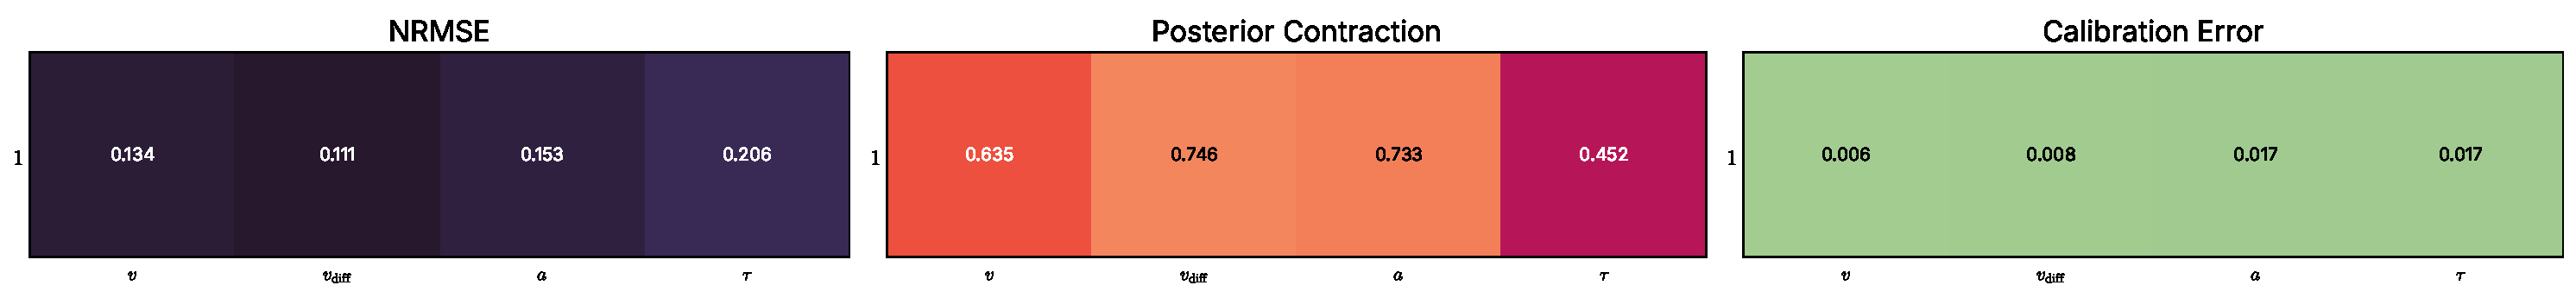
\includegraphics[width=\textwidth]{gap/fixed/bf_metrics.pdf}
    \caption{Metrics}
  \end{subfigure}
  \caption{\textbf{LBA amortization gap: BayesFlow baseline, \emph{fixed} design.} (a) Recovery, (b) calibration, (c) metrics. $s_v$ and $s_\tau$ are fixed at 0 and not estimated; every estimated parameter enters as an intercept only (4 coefficients shown). As in Figure~\ref{fig:app3-gap-lba-intercept-only}; fine-tuned CogFormer on the same datasets: Figure~\ref{fig:app3-finetuned-lba-fixed}.}
  \label{fig:app3-gap-lba-fixed}
\end{figure}

\begin{figure}[p]
  \centering
  \begin{subfigure}{\textwidth}\centering
    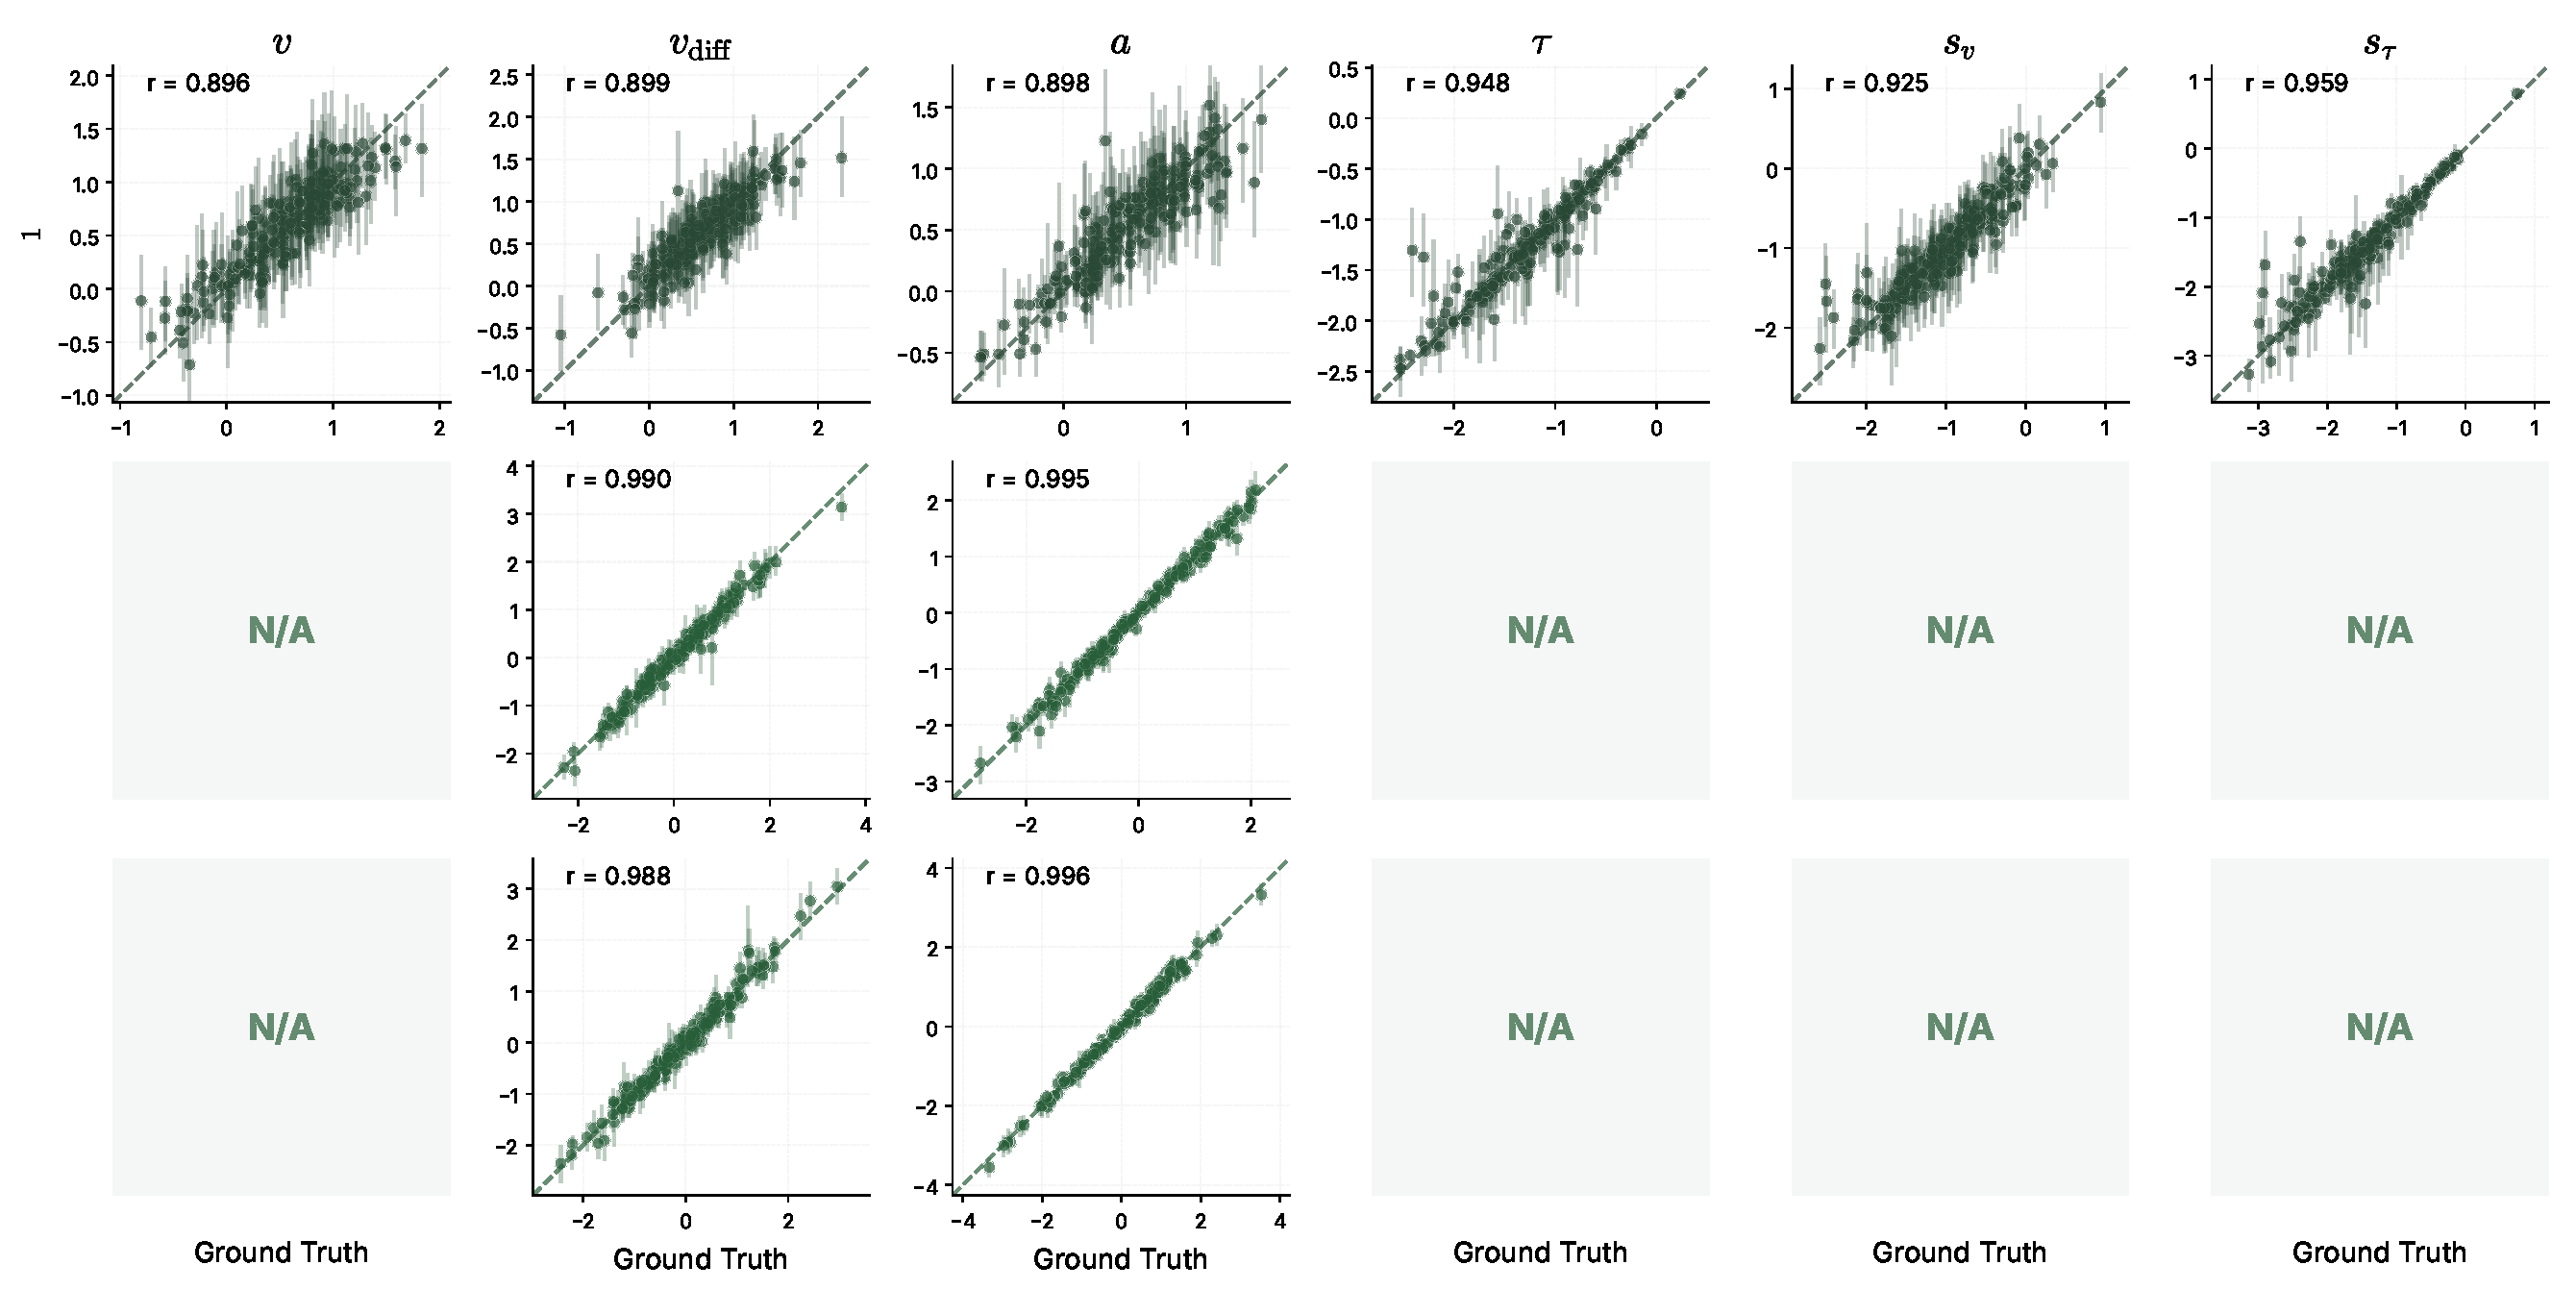
\includegraphics[width=\textwidth,height=0.3\textheight,keepaspectratio]{gap/regressed/bf_recovery.pdf}
    \caption{Recovery}
  \end{subfigure}\\[1ex]
  \begin{subfigure}{\textwidth}\centering
    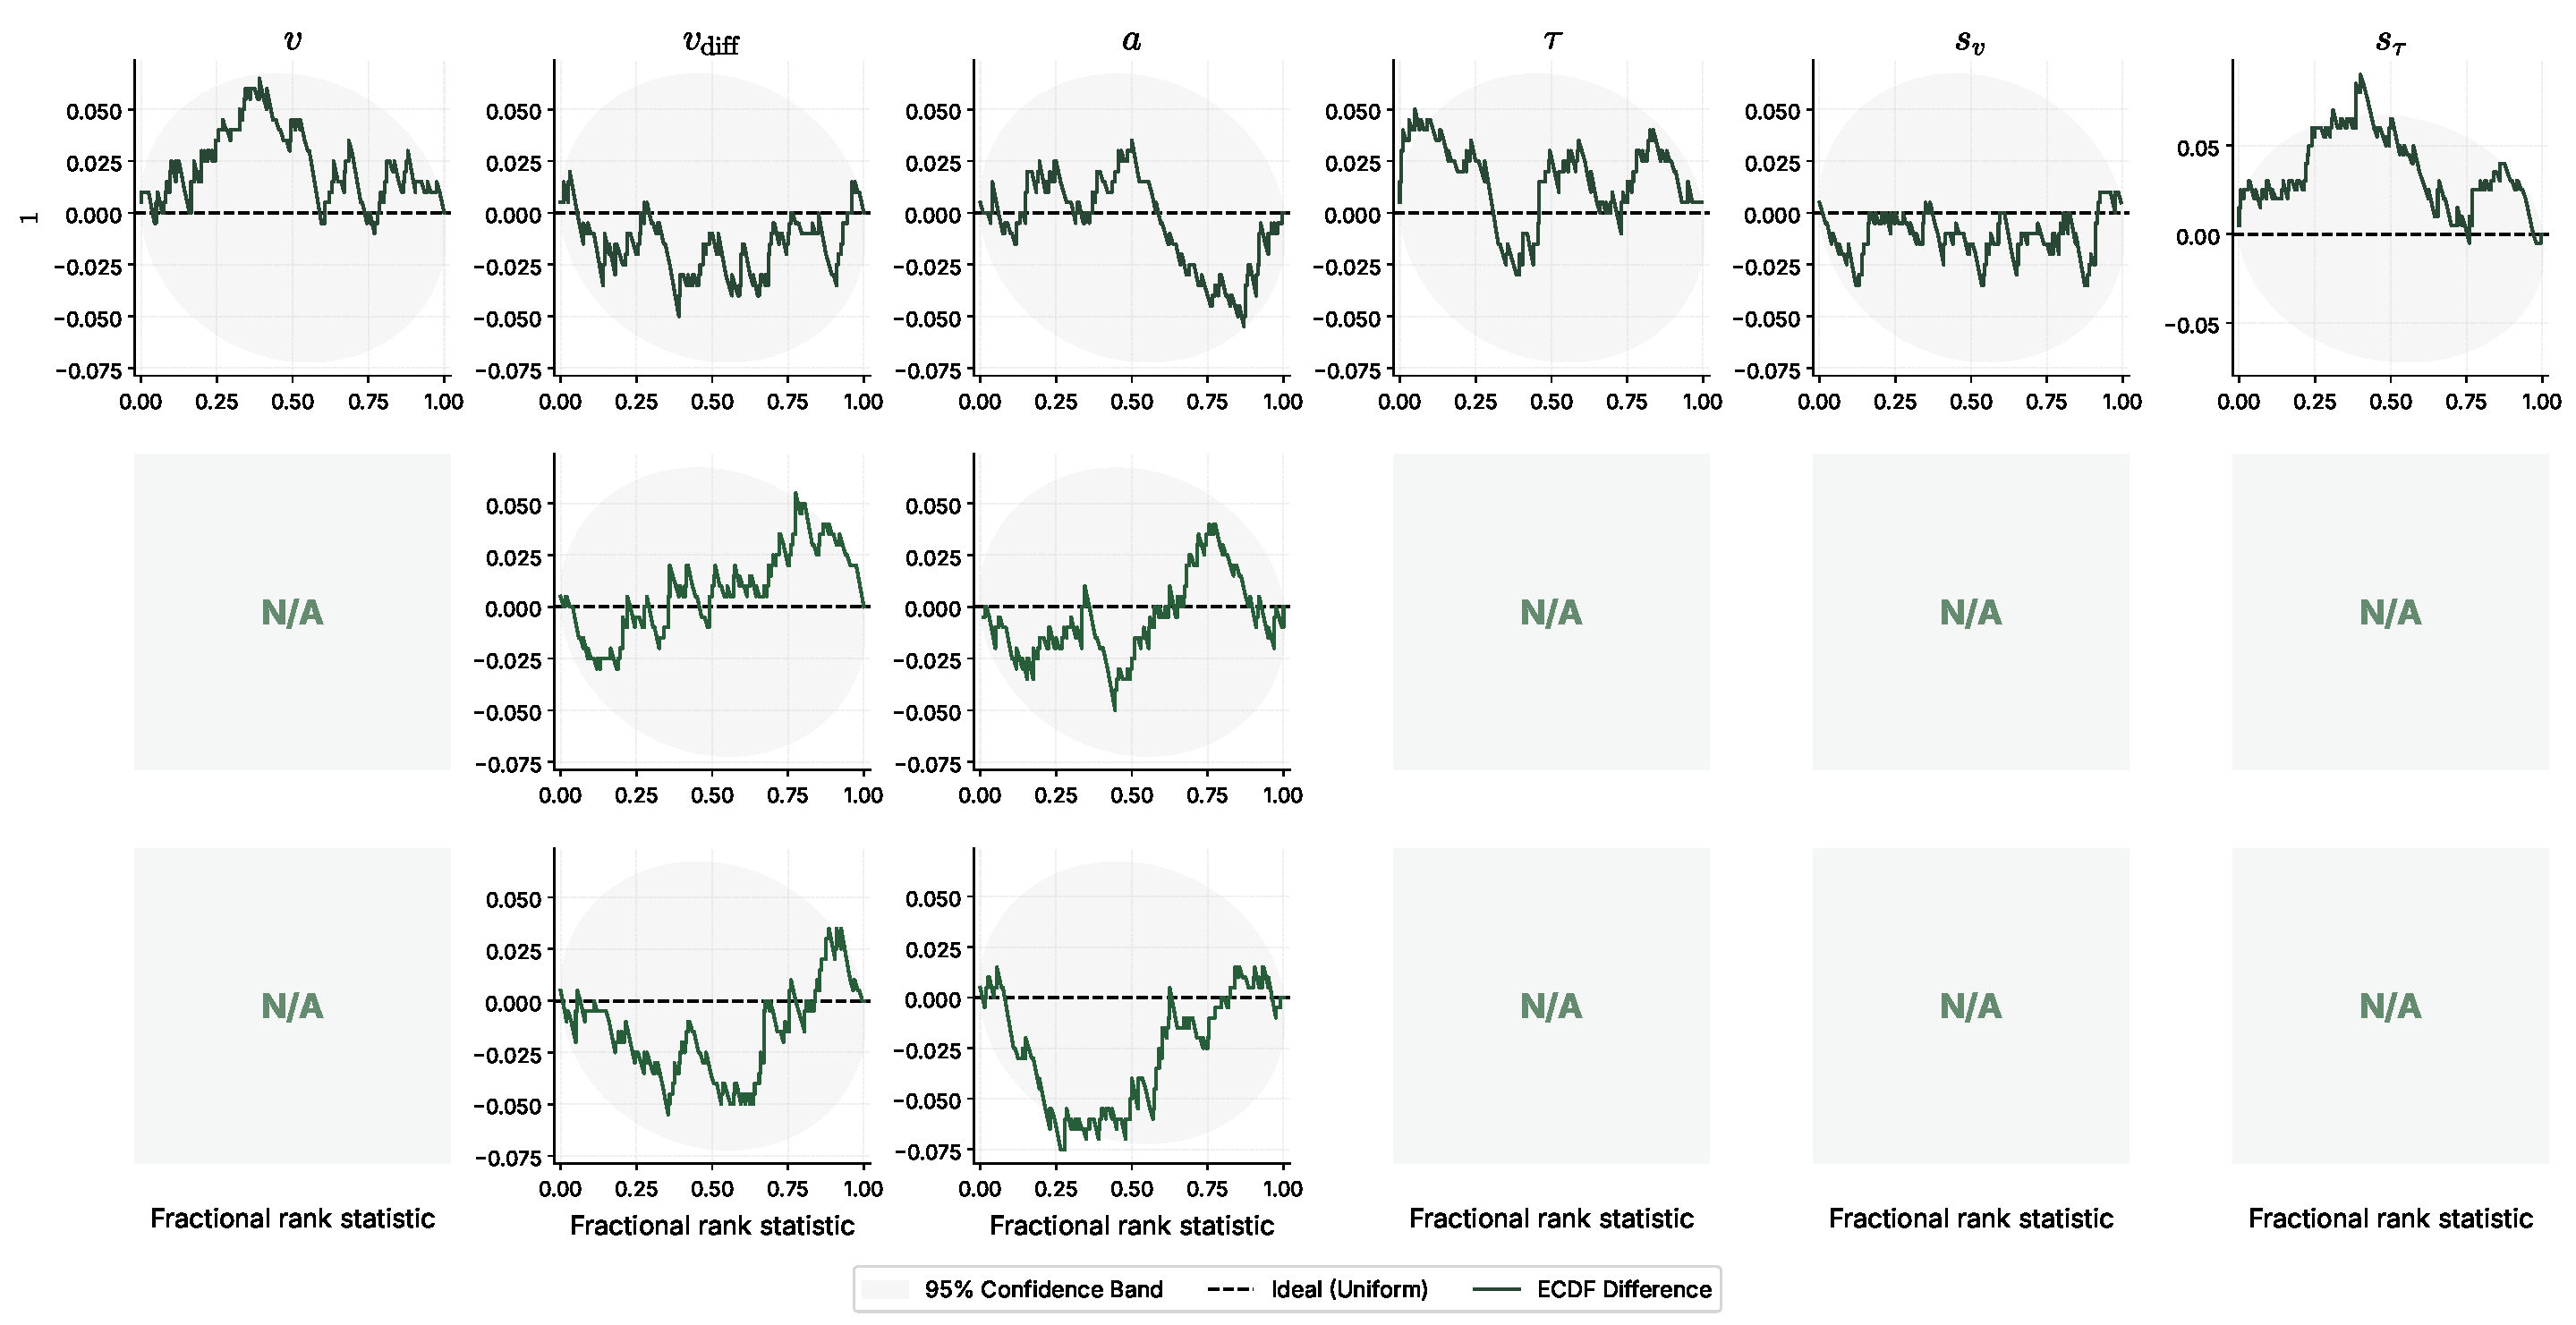
\includegraphics[width=\textwidth,height=0.3\textheight,keepaspectratio]{gap/regressed/bf_ecdf.pdf}
    \caption{Calibration (ECDF)}
  \end{subfigure}\\[1ex]
  \begin{subfigure}{\textwidth}\centering
    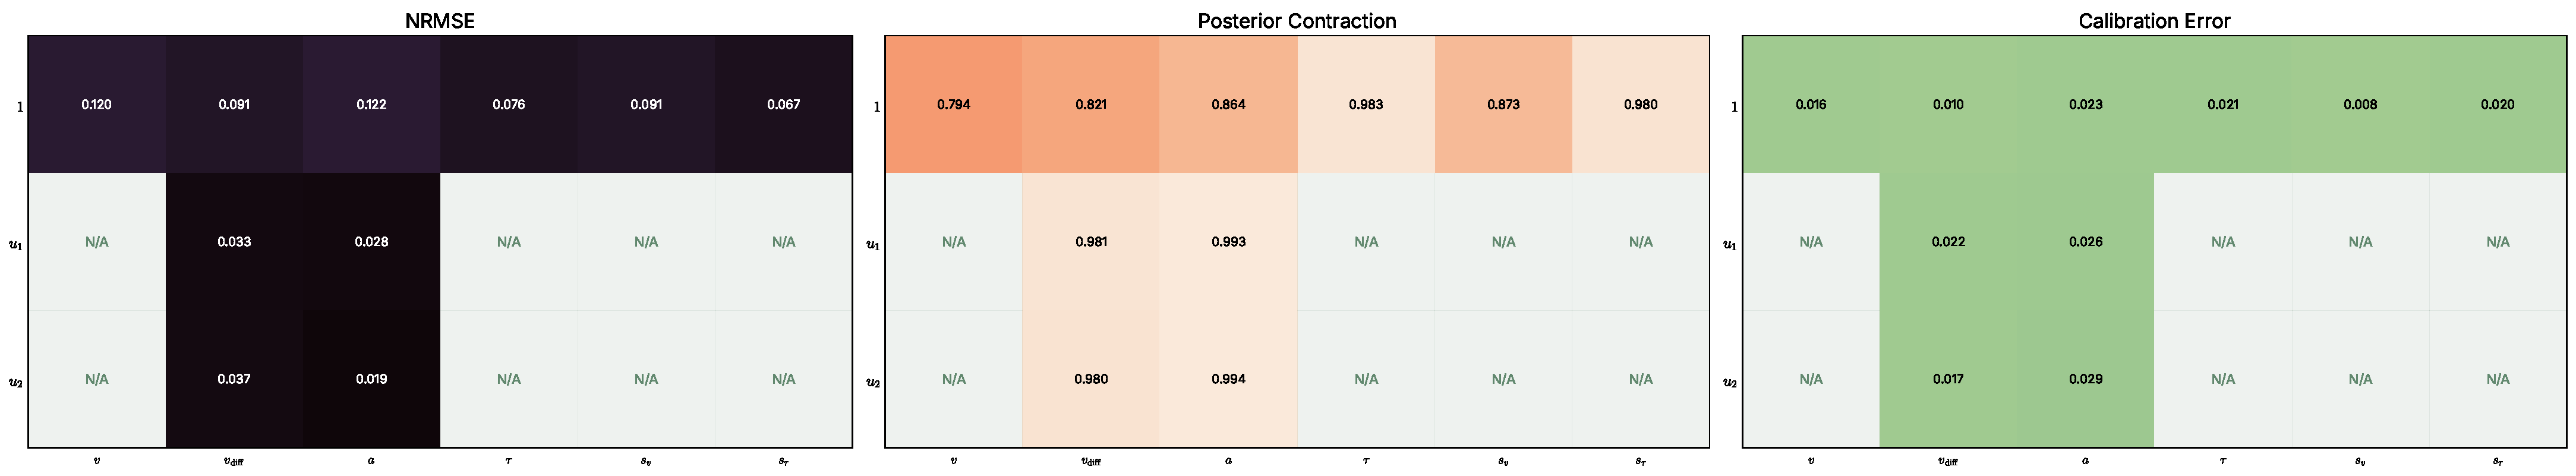
\includegraphics[width=\textwidth]{gap/regressed/bf_metrics.pdf}
    \caption{Metrics}
  \end{subfigure}
  \caption{\textbf{LBA amortization gap: BayesFlow baseline, \emph{regressed} design.} (a) Recovery, (b) calibration, (c) metrics. $v_{\mathrm{diff}}$ and $a$ carry slopes on $u_1$ and $u_2$ (10 coefficients shown). As in Figure~\ref{fig:app3-gap-lba-intercept-only}; fine-tuned CogFormer on the same datasets: Figure~\ref{fig:app3-finetuned-lba-regressed}.}
  \label{fig:app3-gap-lba-regressed}
\end{figure}

\begin{figure}[p]
  \centering
  \begin{subfigure}{\textwidth}\centering
    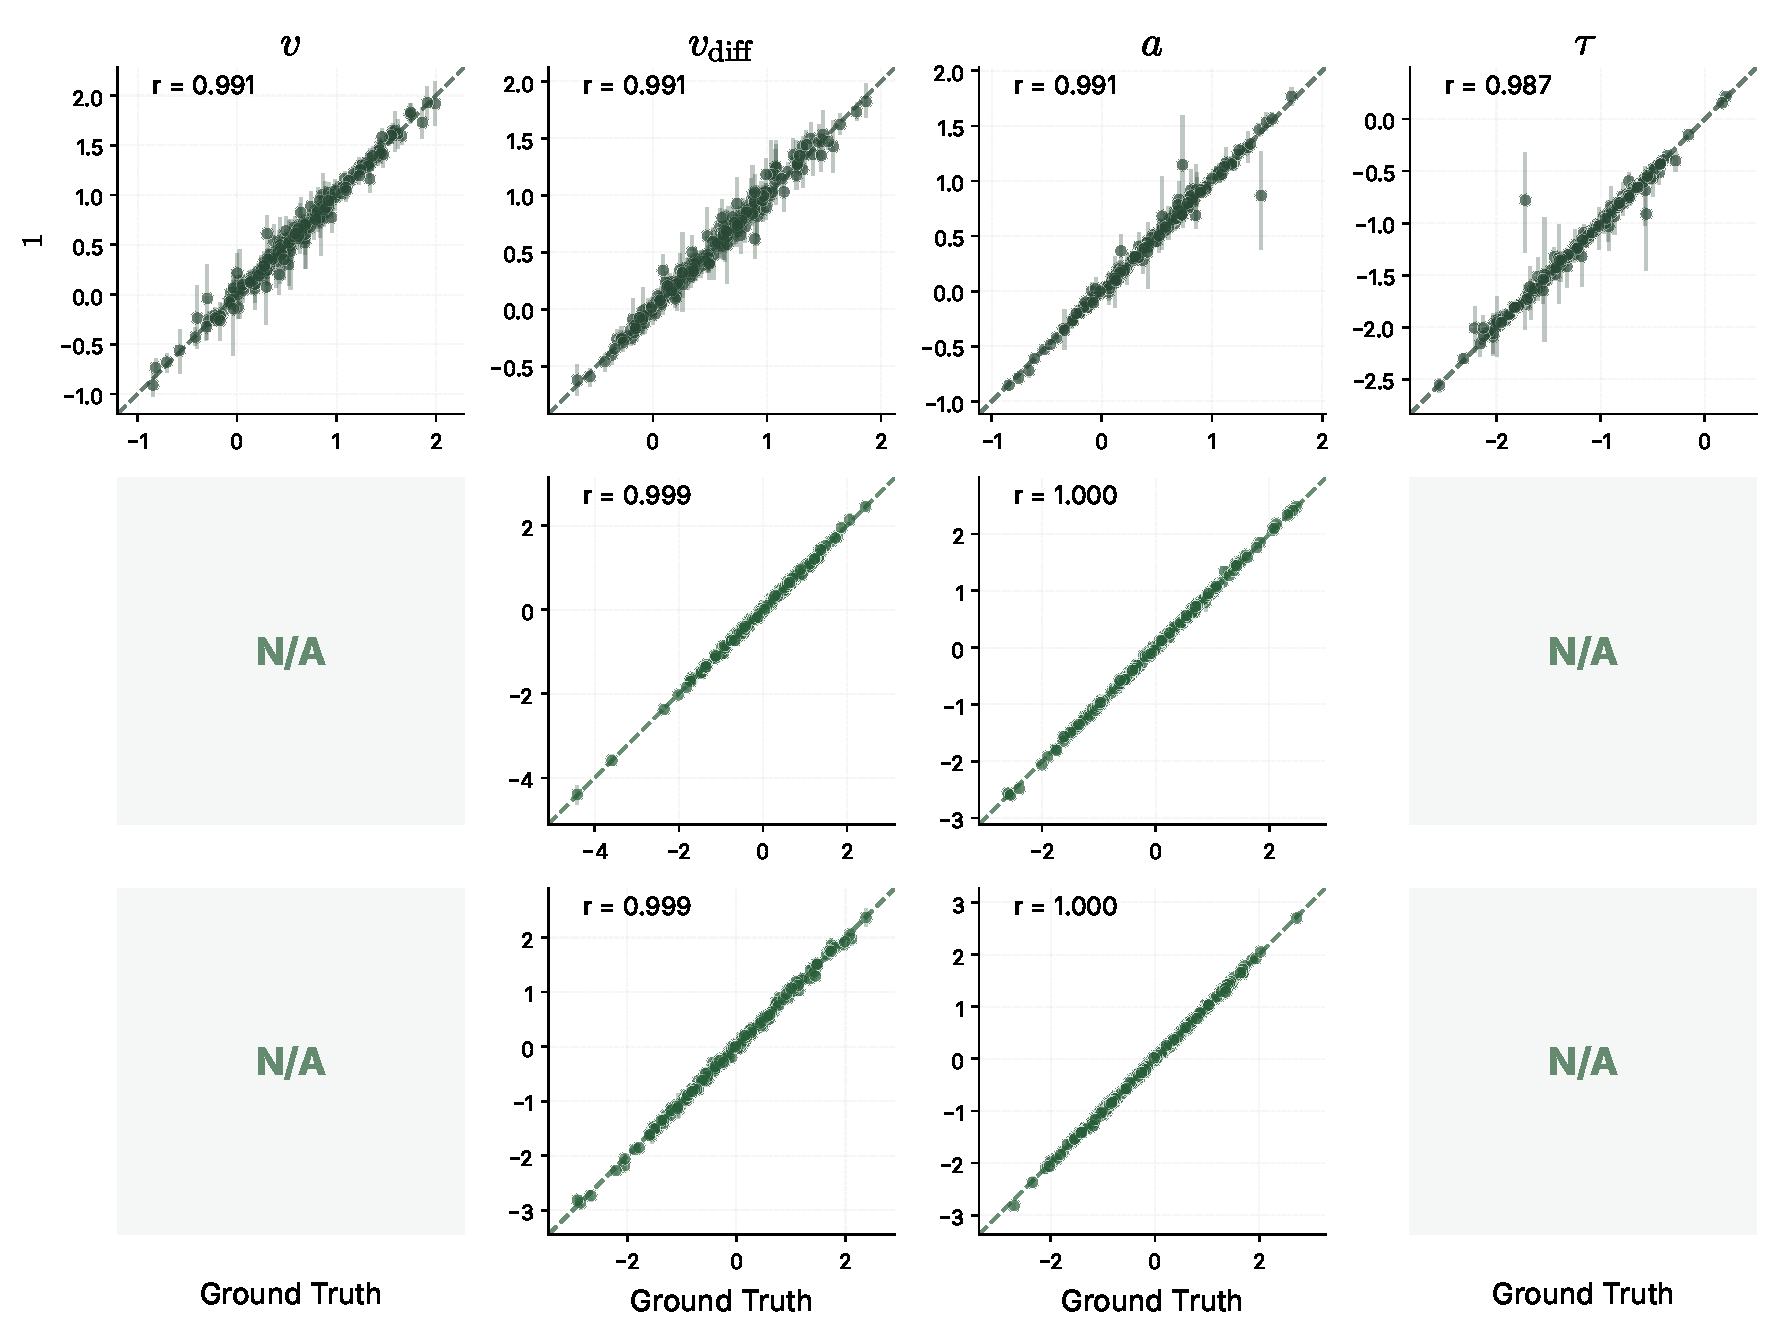
\includegraphics[width=\textwidth,height=0.3\textheight,keepaspectratio]{gap/fixed_regressed/bf_recovery.pdf}
    \caption{Recovery}
  \end{subfigure}\\[1ex]
  \begin{subfigure}{\textwidth}\centering
    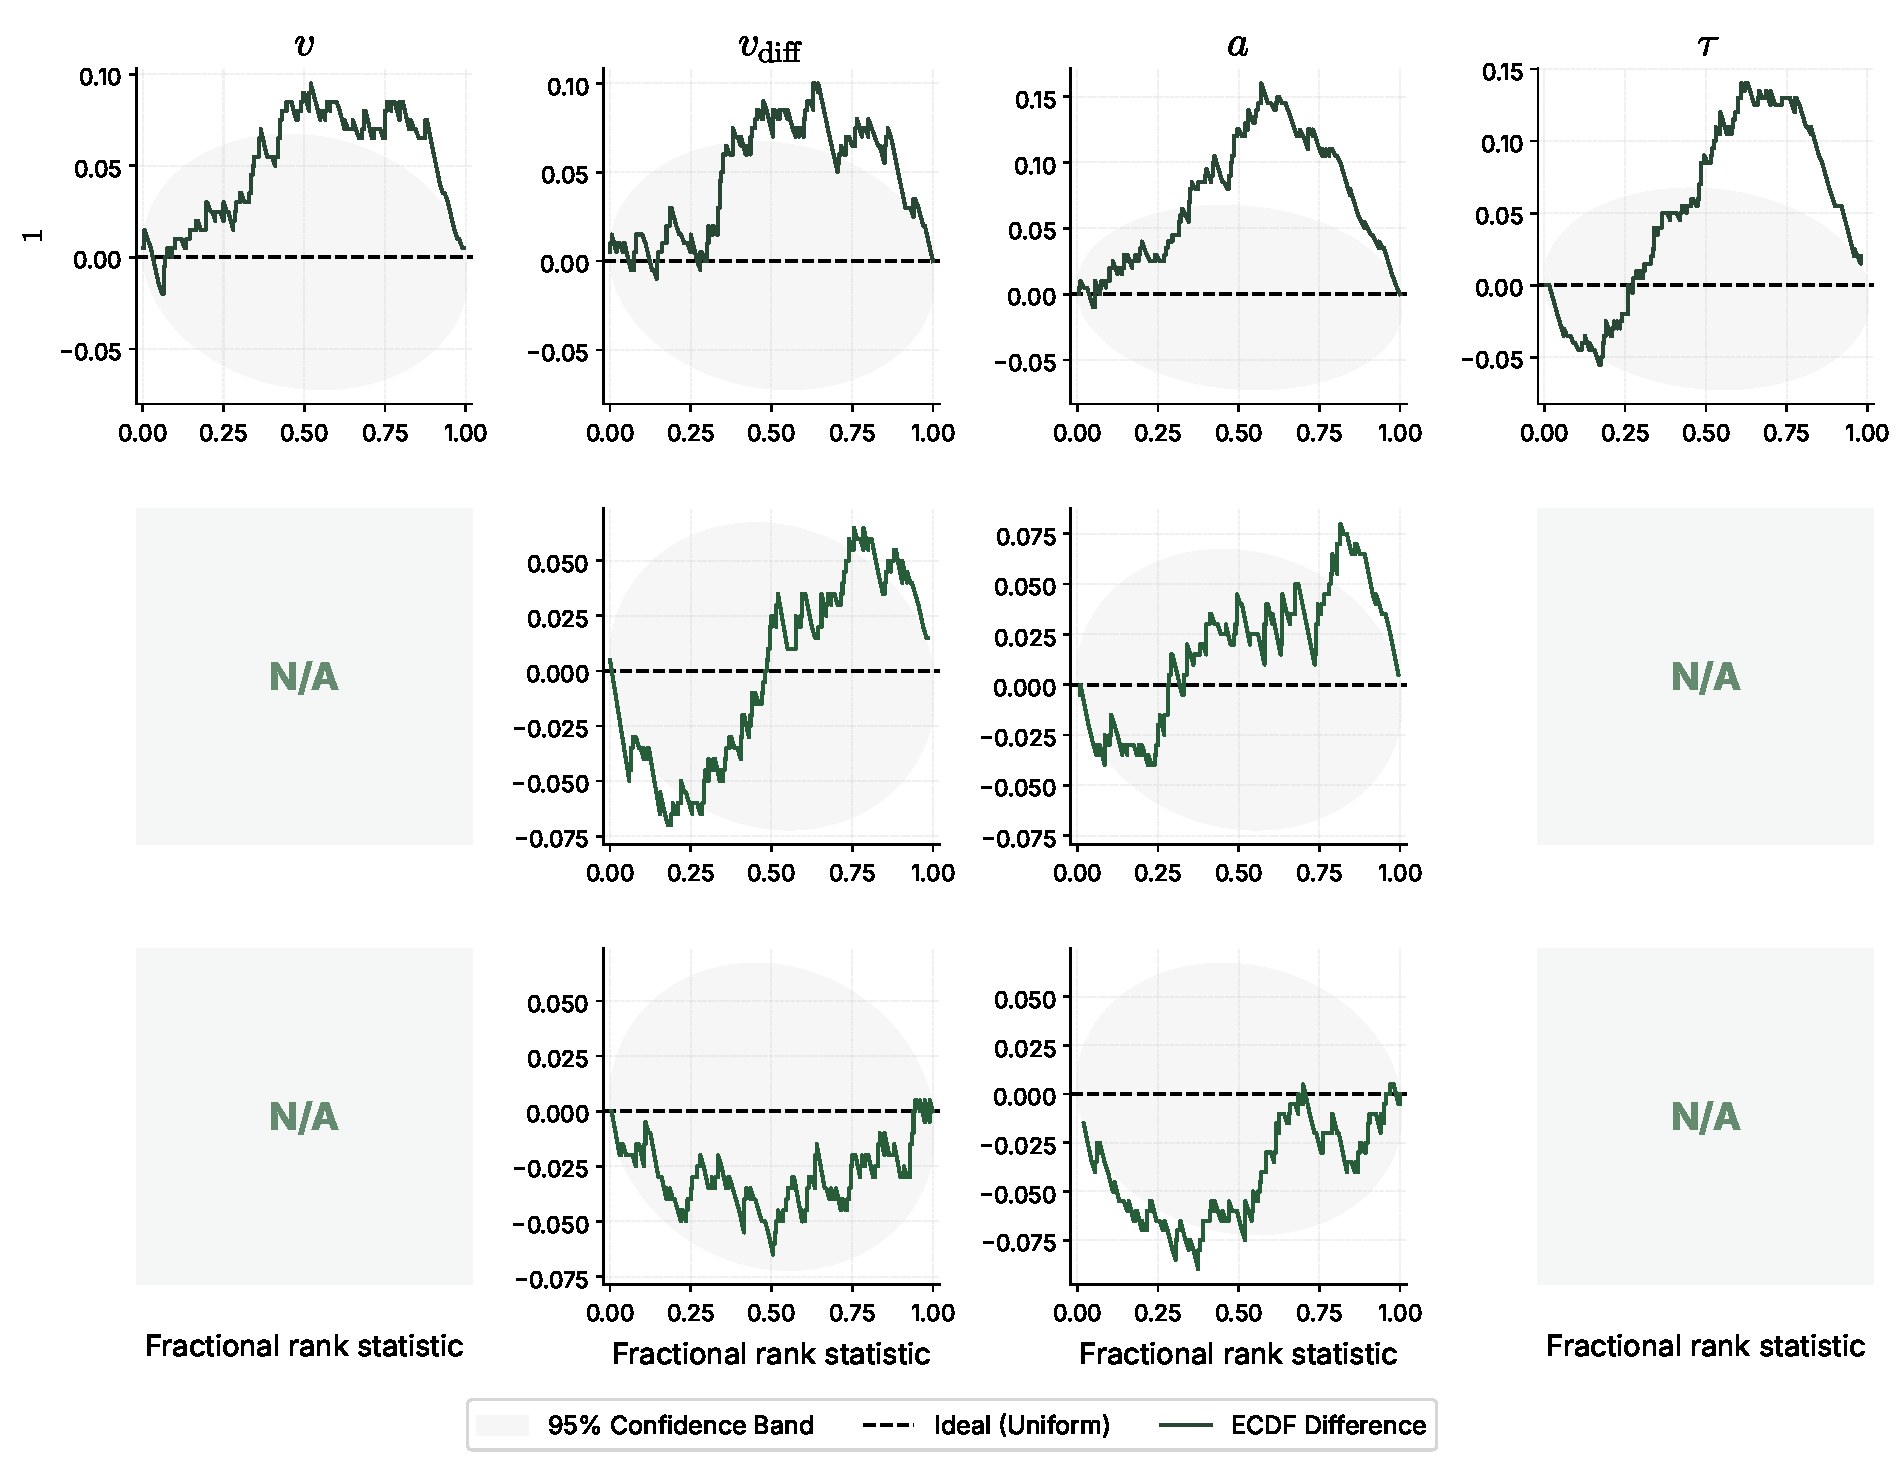
\includegraphics[width=\textwidth,height=0.3\textheight,keepaspectratio]{gap/fixed_regressed/bf_ecdf.pdf}
    \caption{Calibration (ECDF)}
  \end{subfigure}\\[1ex]
  \begin{subfigure}{\textwidth}\centering
    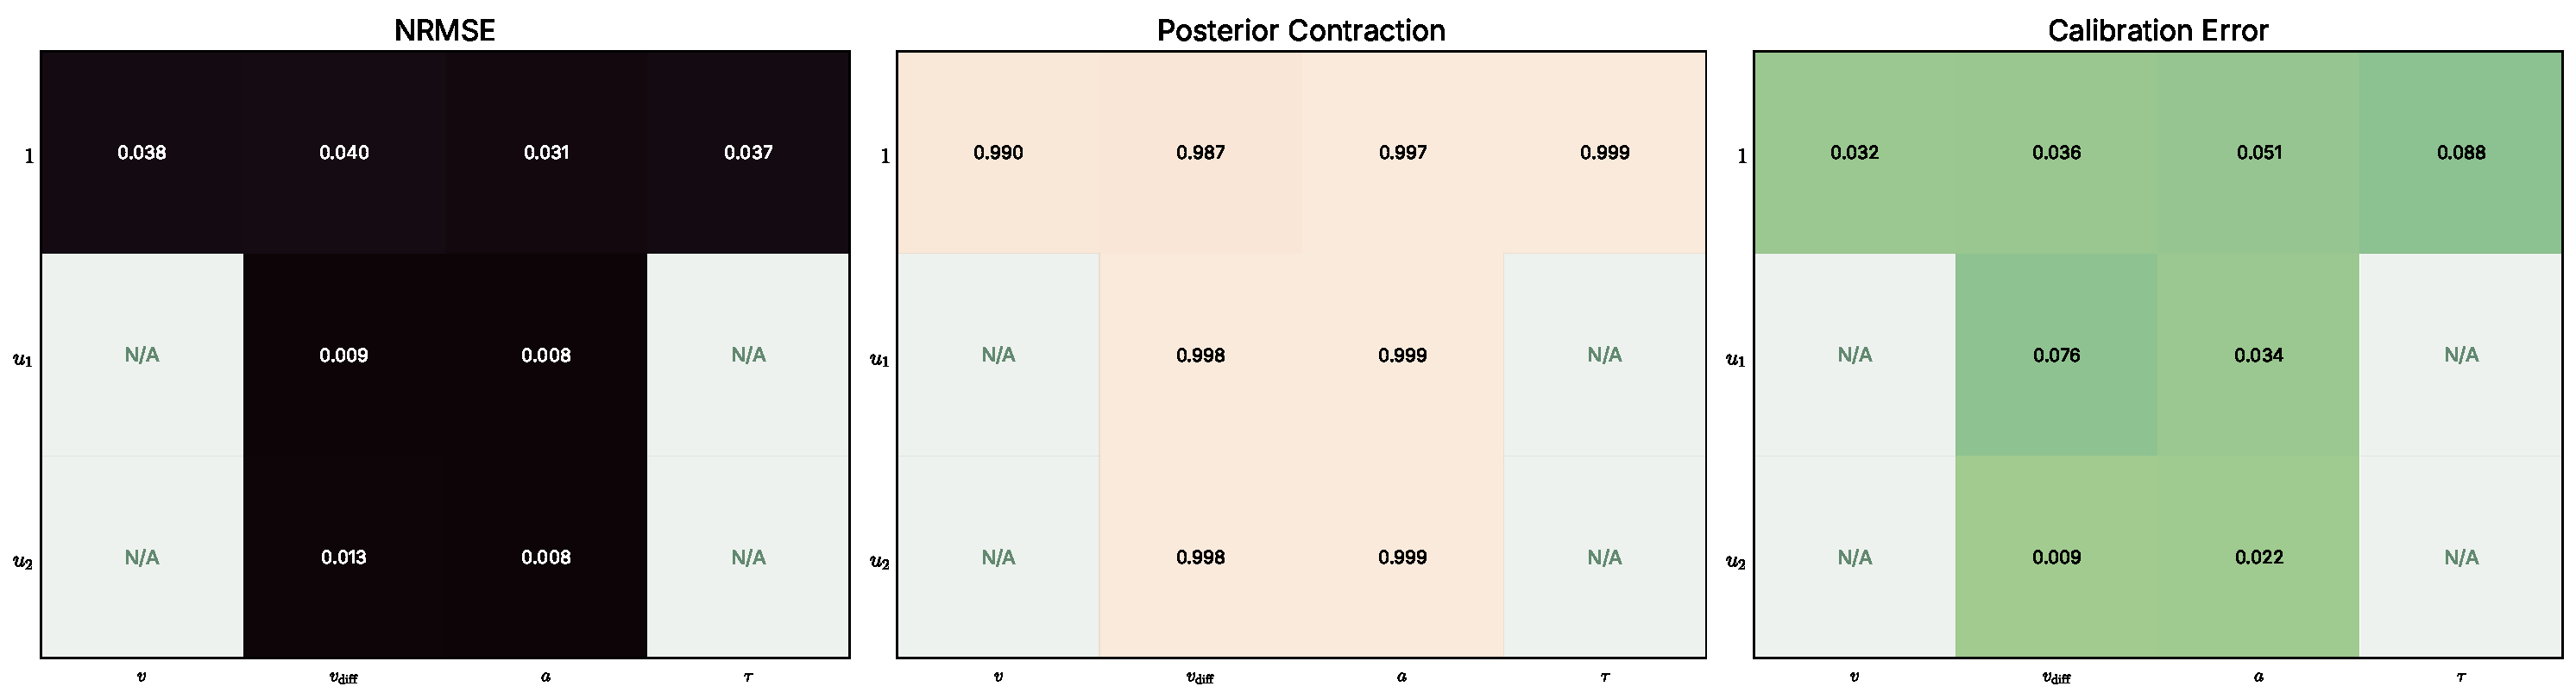
\includegraphics[width=\textwidth]{gap/fixed_regressed/bf_metrics.pdf}
    \caption{Metrics}
  \end{subfigure}
  \caption{\textbf{LBA amortization gap: BayesFlow baseline, \emph{fixed + regressed} design.} (a) Recovery, (b) calibration, (c) metrics. $s_v$ and $s_\tau$ are fixed at 0 and not estimated; $v_{\mathrm{diff}}$ and $a$ carry slopes on $u_1$ and $u_2$ (8 coefficients shown). As in Figure~\ref{fig:app3-gap-lba-intercept-only}; fine-tuned CogFormer on the same datasets: Figure~\ref{fig:app3-finetuned-lba-fixed-regressed}.}
  \label{fig:app3-gap-lba-fixed-regressed}
\end{figure}

\begin{figure}[p]
  \centering
  \begin{subfigure}{\textwidth}\centering
    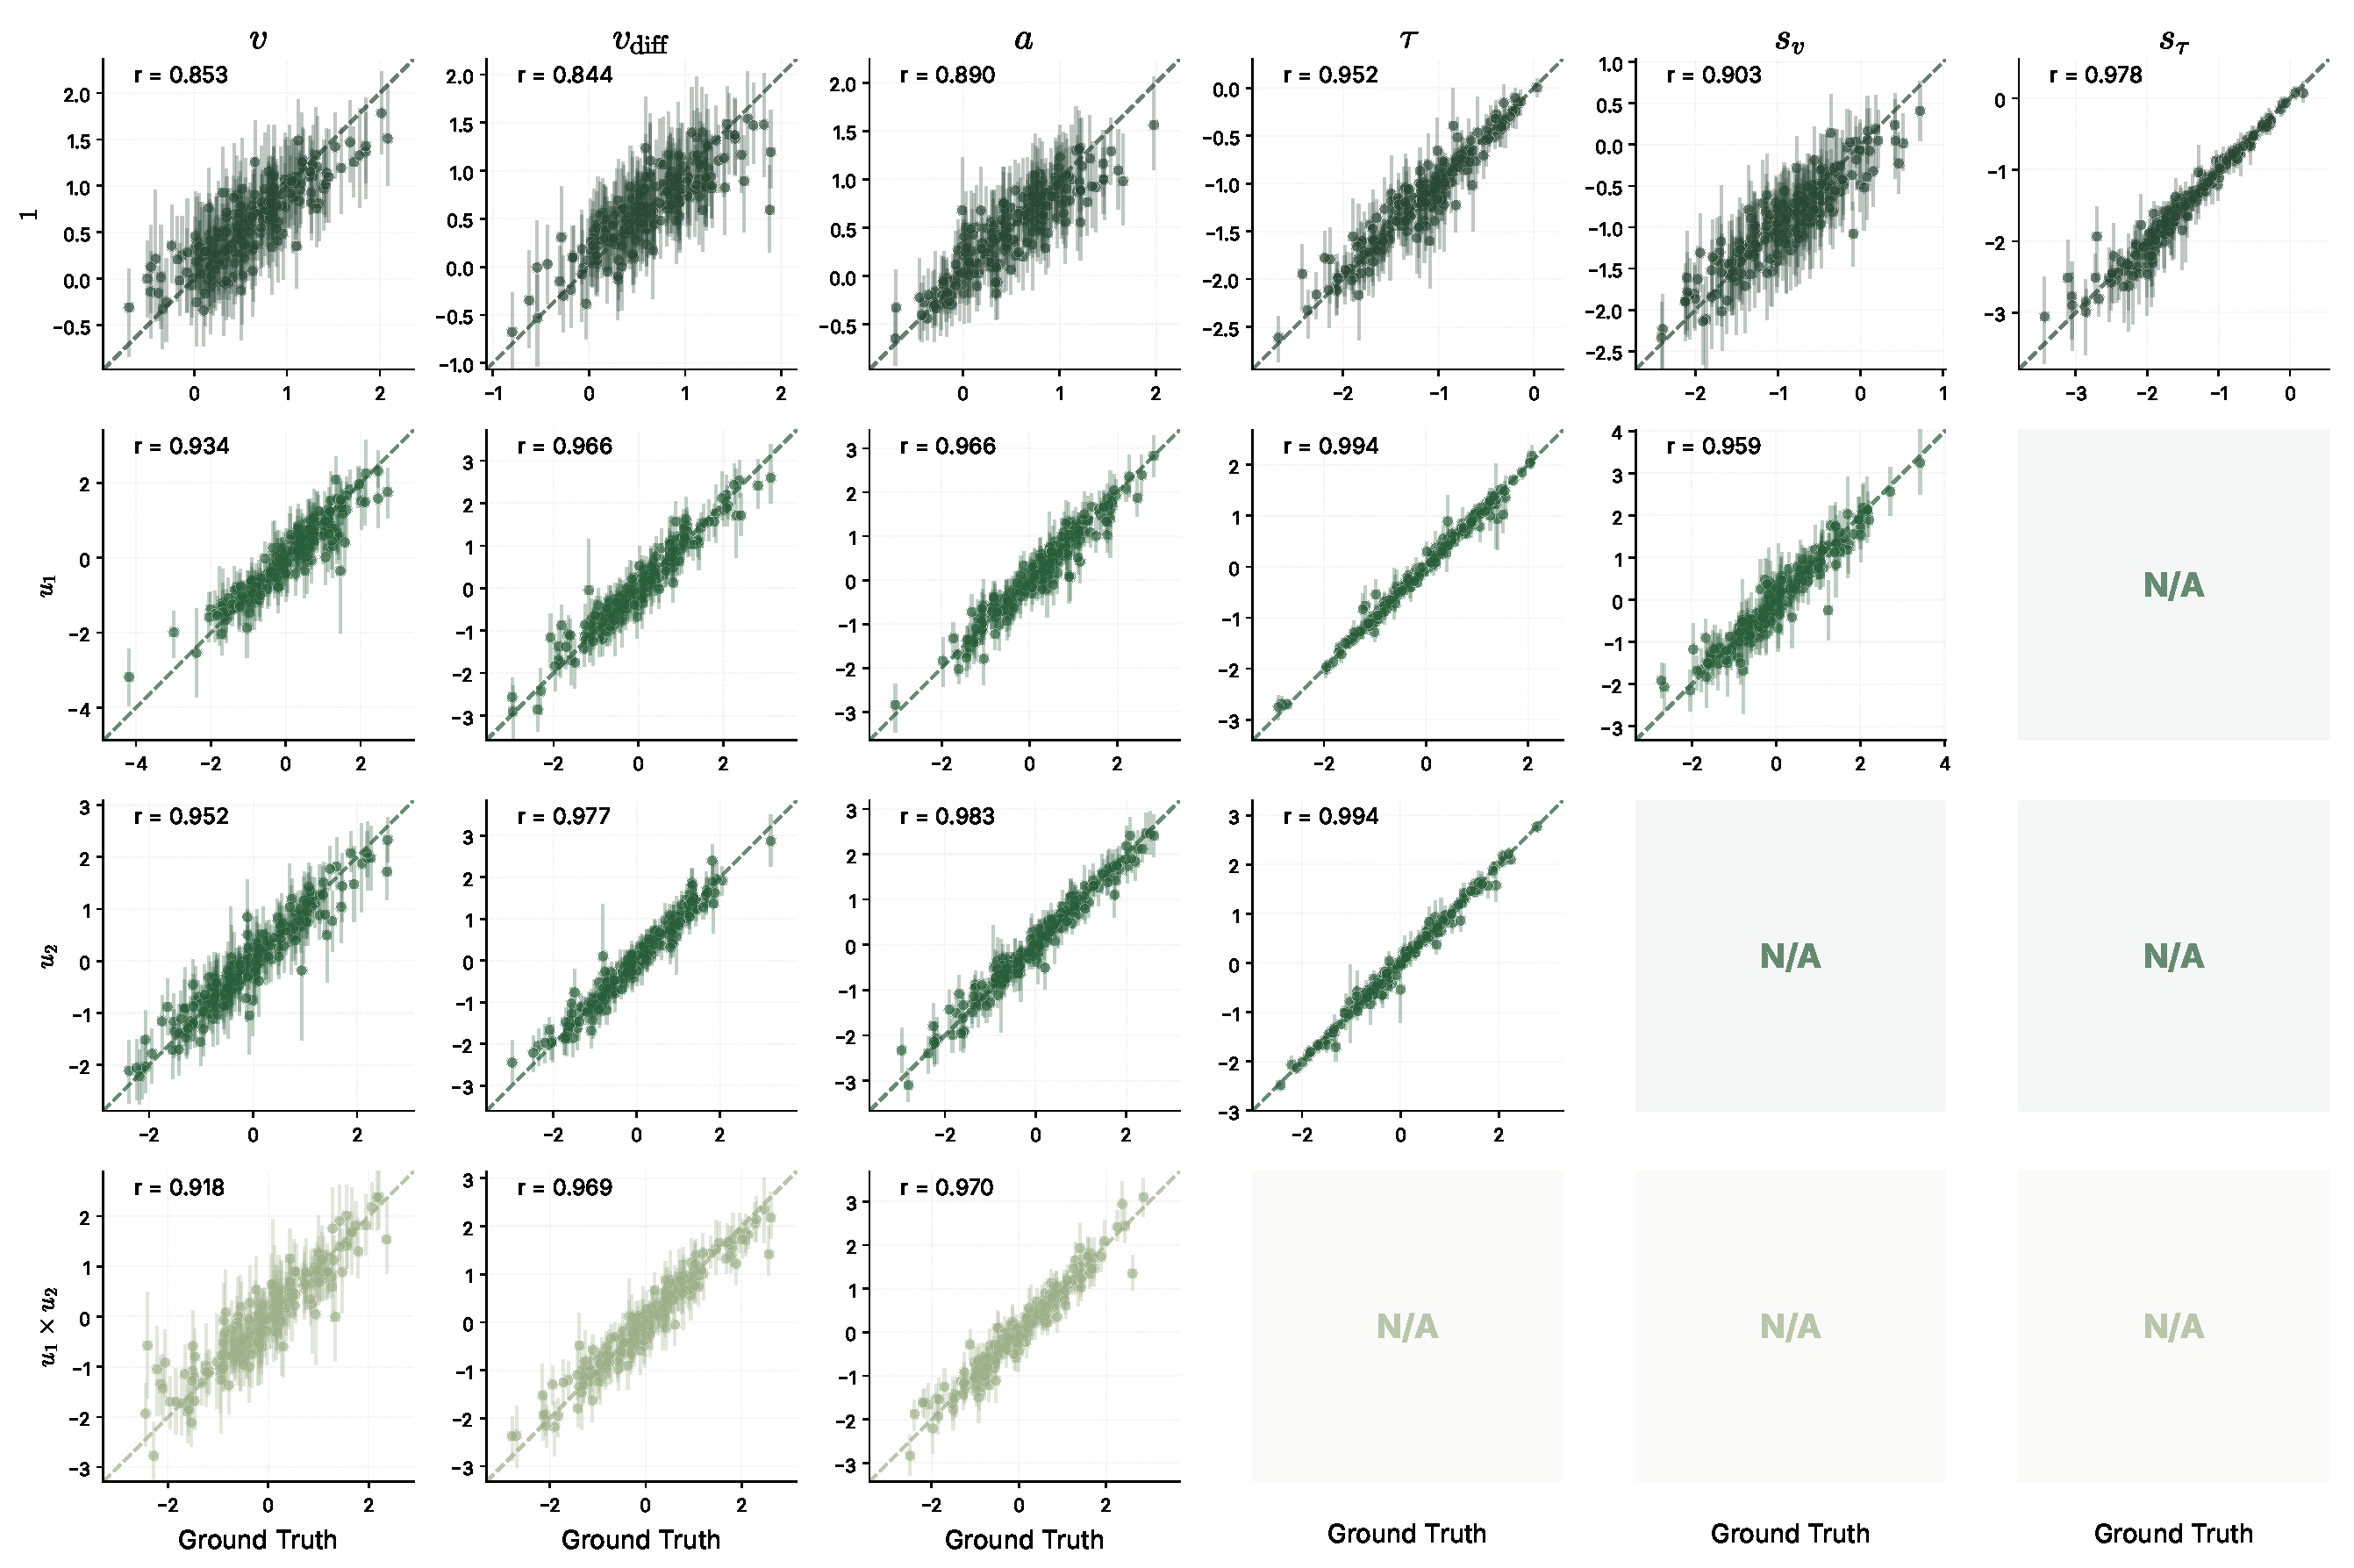
\includegraphics[width=\textwidth,height=0.3\textheight,keepaspectratio]{gap/interaction/bf_recovery.pdf}
    \caption{Recovery}
  \end{subfigure}\\[1ex]
  \begin{subfigure}{\textwidth}\centering
    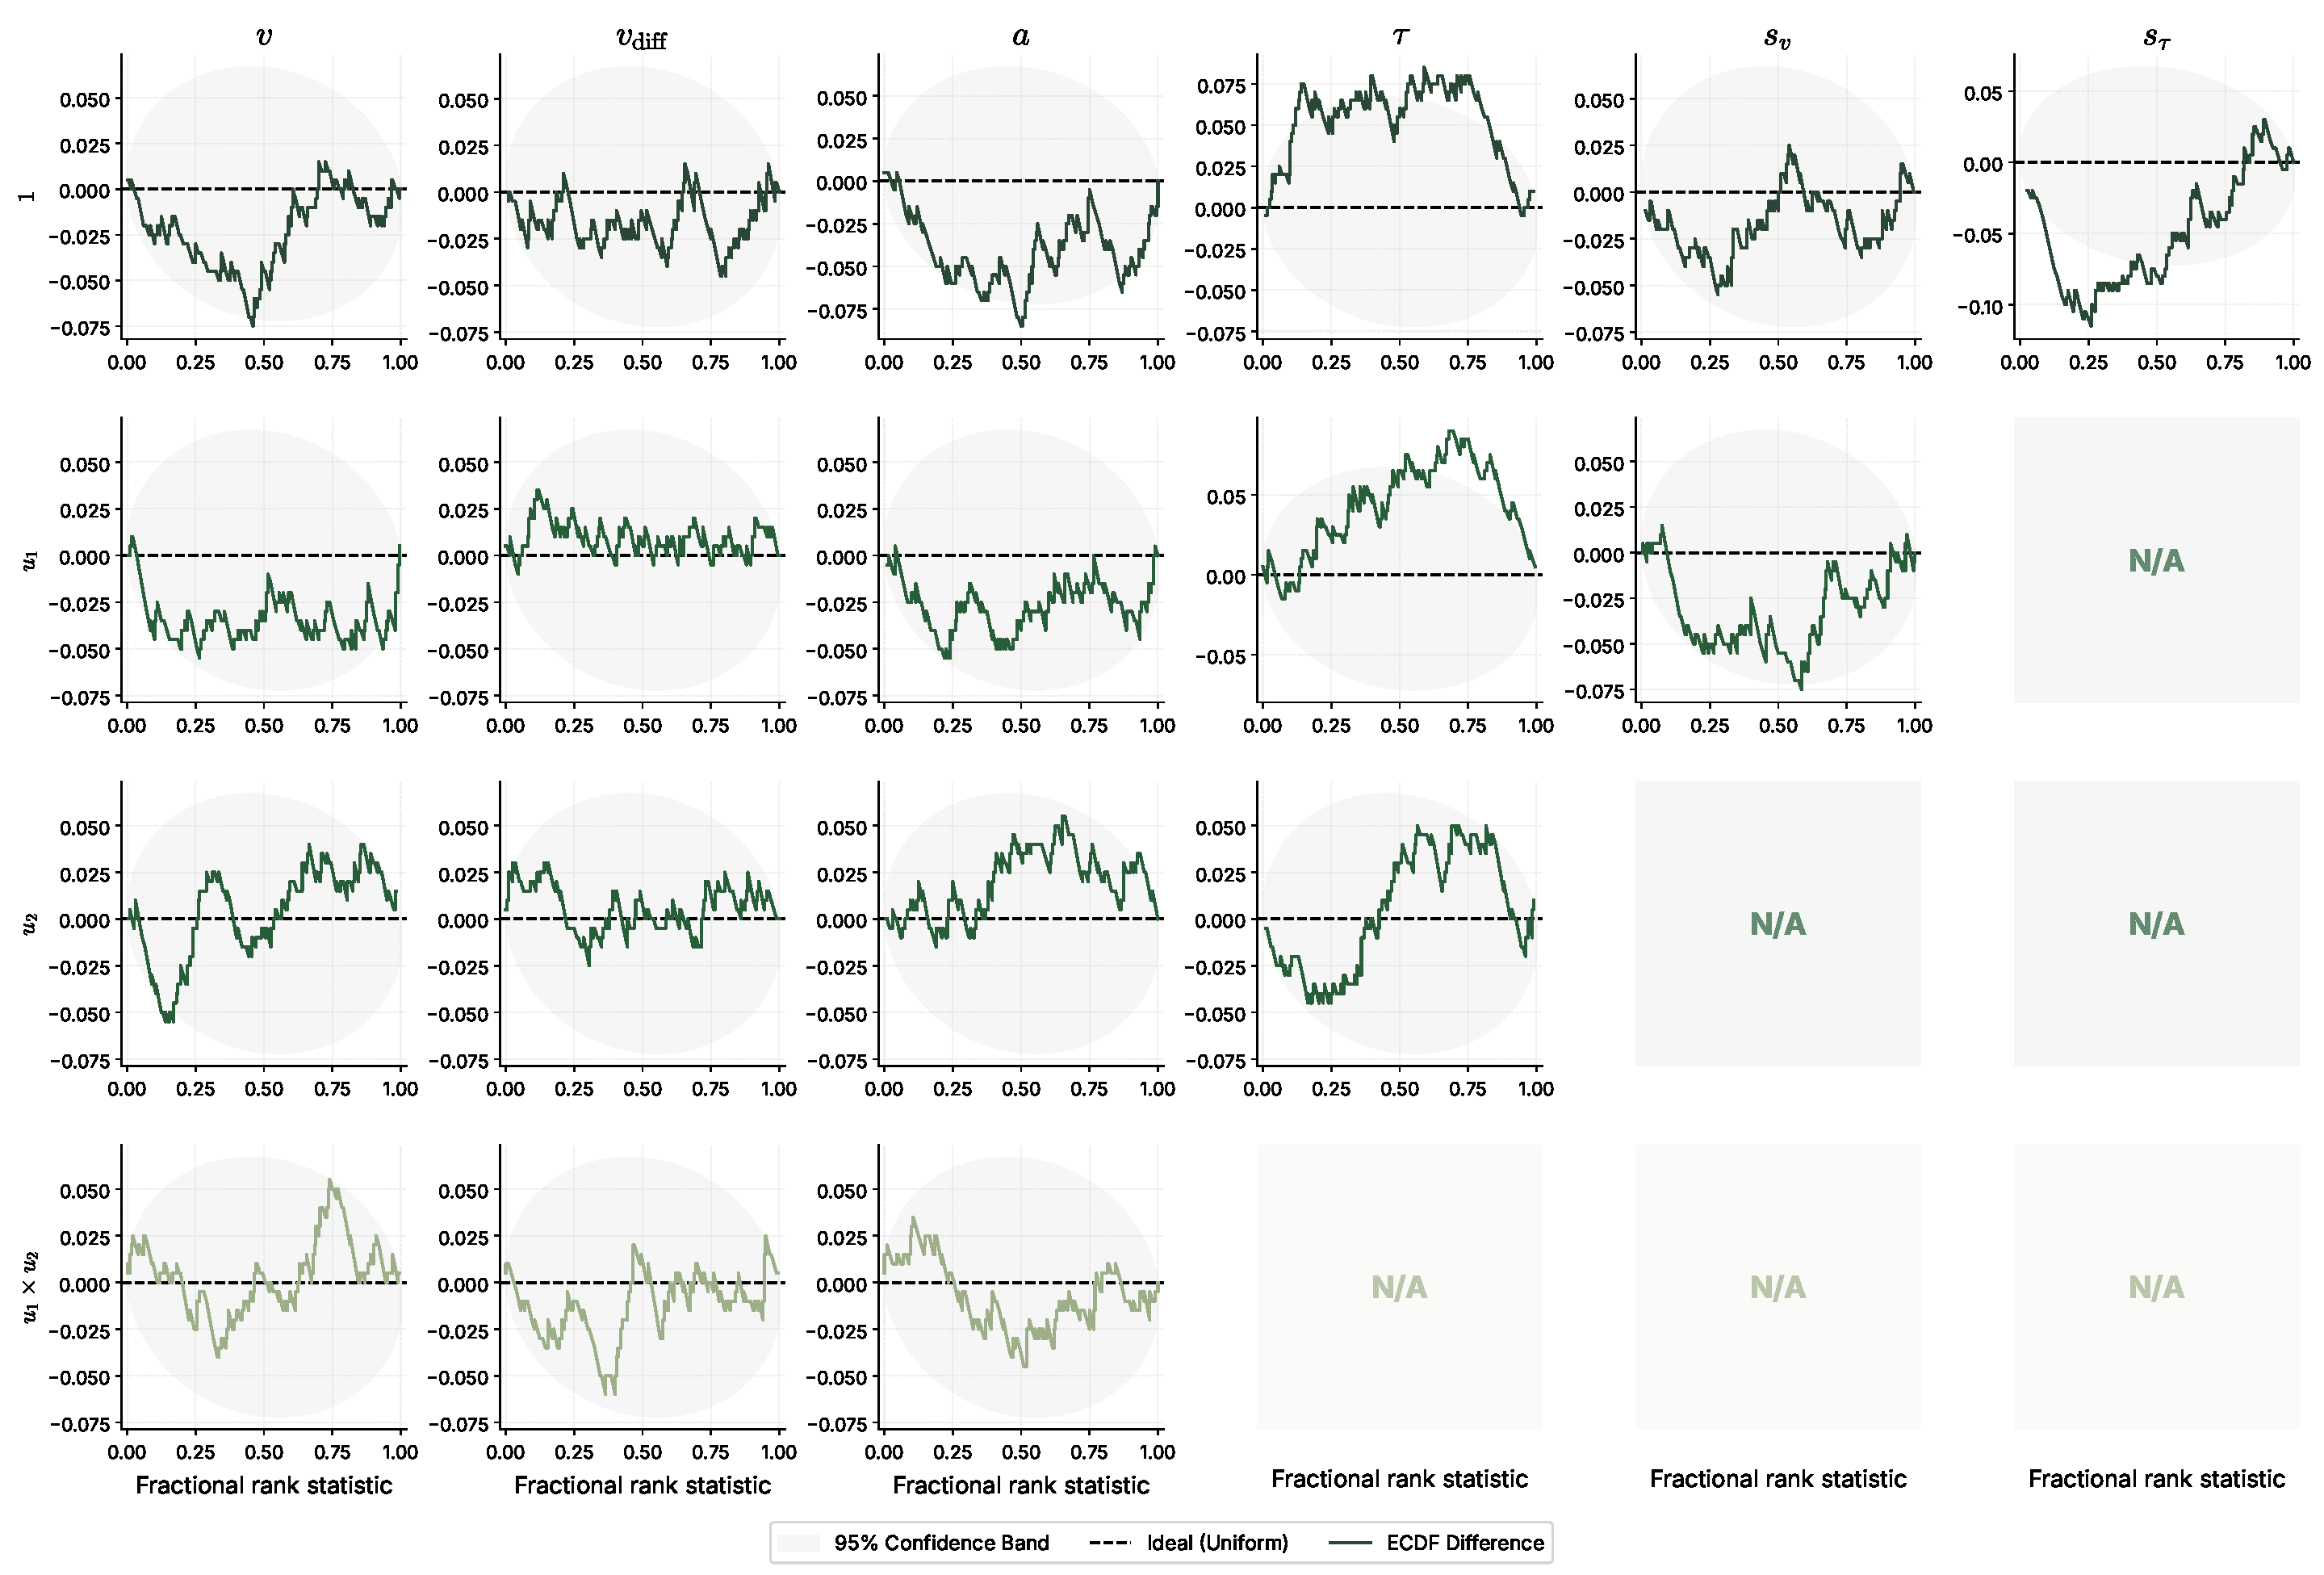
\includegraphics[width=\textwidth,height=0.3\textheight,keepaspectratio]{gap/interaction/bf_ecdf.pdf}
    \caption{Calibration (ECDF)}
  \end{subfigure}\\[1ex]
  \begin{subfigure}{\textwidth}\centering
    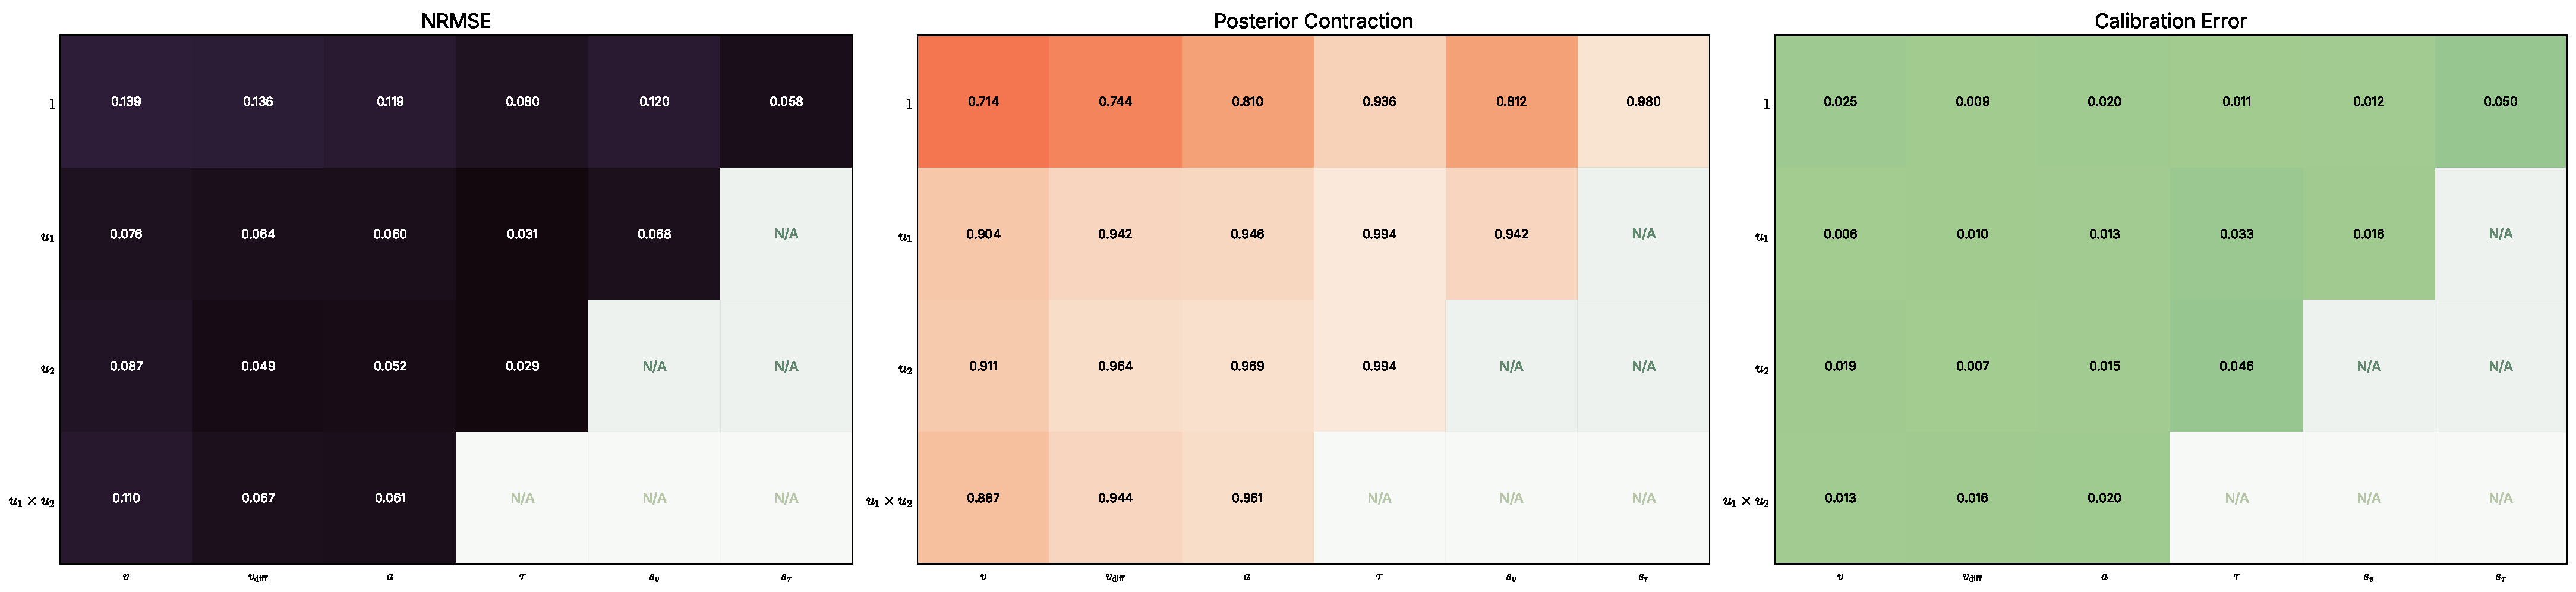
\includegraphics[width=\textwidth]{gap/interaction/bf_metrics.pdf}
    \caption{Metrics}
  \end{subfigure}
  \caption{\textbf{LBA amortization gap: BayesFlow baseline, \emph{interaction} design.} (a) Recovery, (b) calibration, (c) metrics. $v$, $v_{\mathrm{diff}}$, $a$, $\tau$ and $s_v$ carry slopes on $u_1$; $v$, $v_{\mathrm{diff}}$, $a$ and $\tau$ carry slopes on $u_2$; $v$, $v_{\mathrm{diff}}$ and $a$ on the product $u_1 u_2$ (18 coefficients shown). As in Figure~\ref{fig:app3-gap-lba-intercept-only}; fine-tuned CogFormer on the same datasets: Figure~\ref{fig:app3-finetuned-lba-interaction}.}
  \label{fig:app3-gap-lba-interaction}
\end{figure}

% ── 7. LBA on empirical data (free variant: s_v, s_tau as estimated) ──

\begin{figure}[p]
  \centering
  \begin{subfigure}{\textwidth}\centering
    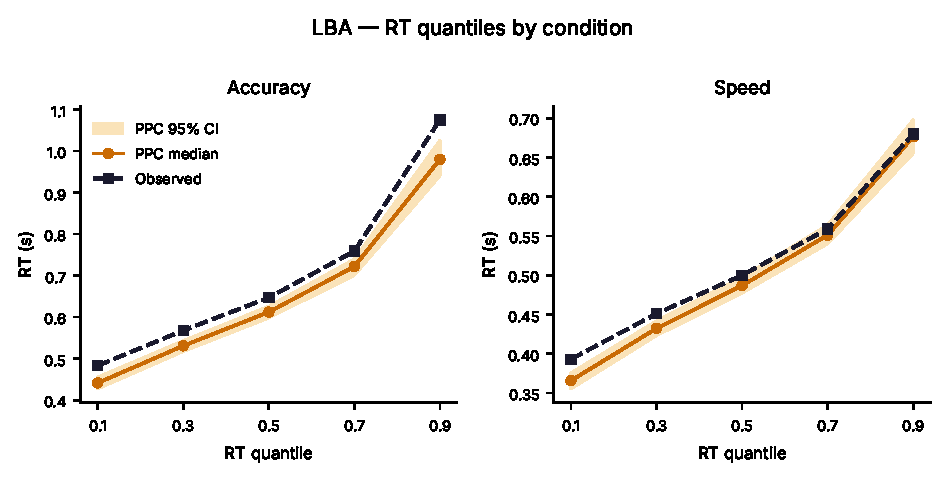
\includegraphics[width=\textwidth,height=0.18\textheight,keepaspectratio]{ppc/free/rt_quantiles_condition.pdf}
    \caption{RT quantiles}
  \end{subfigure}\\[0.5ex]
  \begin{subfigure}{\textwidth}\centering
    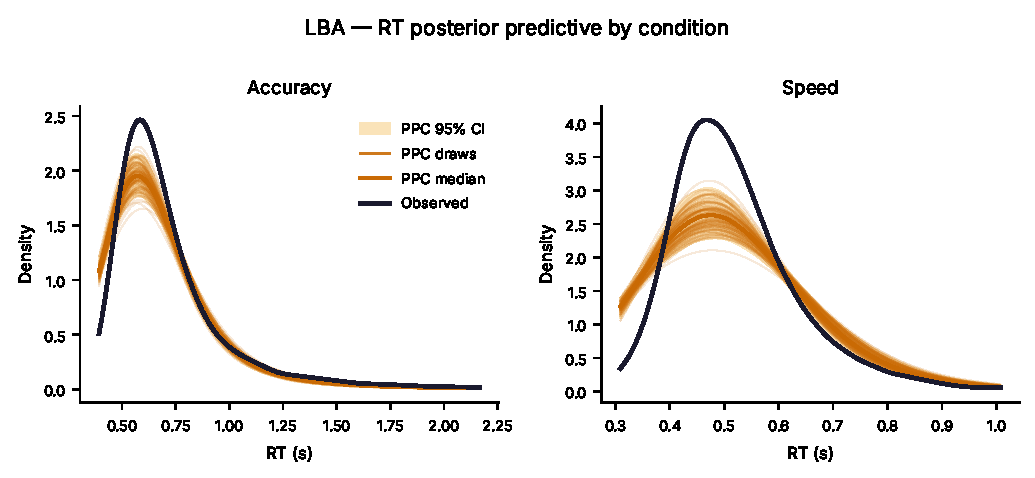
\includegraphics[width=\textwidth,height=0.18\textheight,keepaspectratio]{ppc/free/rt_ppc_condition.pdf}
    \caption{RT densities}
  \end{subfigure}
  \caption{\textbf{LBA on empirical lexical-decision data: posterior predictive check by speed/accuracy condition.} The fine-tuned network applied to the lexical-decision data of Wagenmakers, Ratcliff, Gomez and McKoon (2008) (17 subjects; 792--1920 trials each, median 1917), fitted per subject with an intercept and the speed/accuracy condition ($\pm 0.5$) on $v$, $v_{\mathrm{diff}}$, $a$ and $\tau$; lexicality enters only through stimulus coding, the correct response's accumulator being the favoured one. Each of 500 posterior draws per subject simulates that subject's own trials (contamination included), and the simulated trials are pooled over subjects, giving one predictive data set per draw; correct and error responses are pooled. (a) The 0.1, 0.3, 0.5, 0.7 and 0.9 RT quantiles per level: observed (black squares, dashed) against the predictive median (line) and its 95\% interval across draws (band). (b) RT densities: observed (dark line) against individual predictive draws (thin lines), their pointwise median and 95\% band; Gaussian kernel density estimates (Silverman bandwidth), plotted between the 1st and 99th percentiles of the observed RTs. Panels have independent $y$-axes. Figures~\ref{fig:app3-realdata-frequency} and~\ref{fig:app3-realdata-lexicality} show the same check by word frequency and by lexicality.}
  \label{fig:app3-realdata-condition}
\end{figure}

\begin{figure}[p]
  \centering
  \begin{subfigure}{\textwidth}\centering
    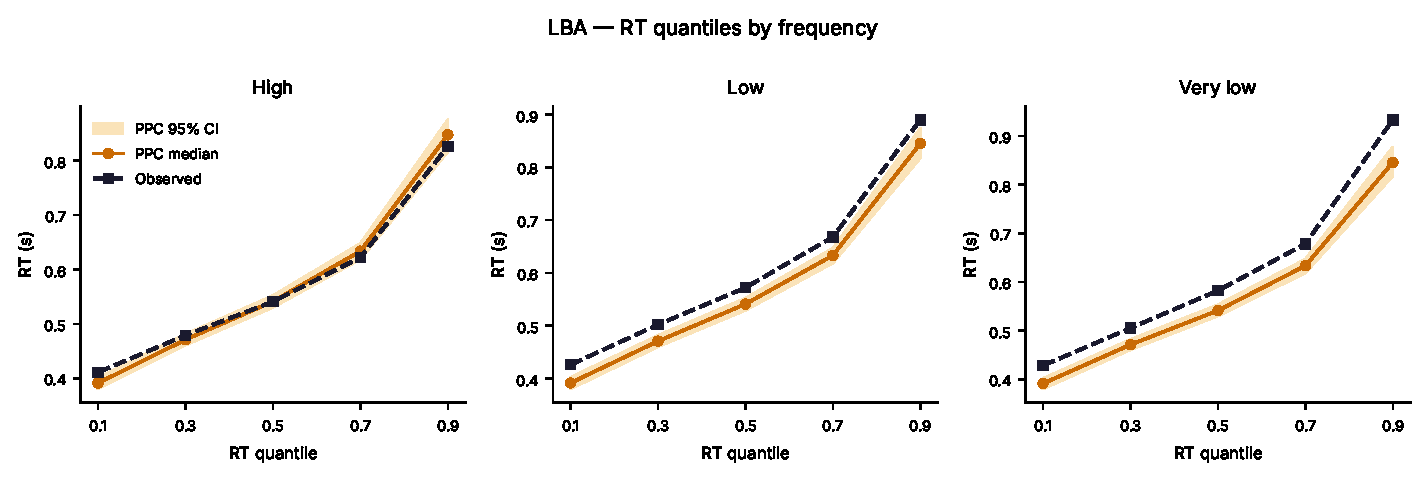
\includegraphics[width=\textwidth,height=0.18\textheight,keepaspectratio]{ppc/free/rt_quantiles_frequency.pdf}
    \caption{RT quantiles}
  \end{subfigure}\\[0.5ex]
  \begin{subfigure}{\textwidth}\centering
    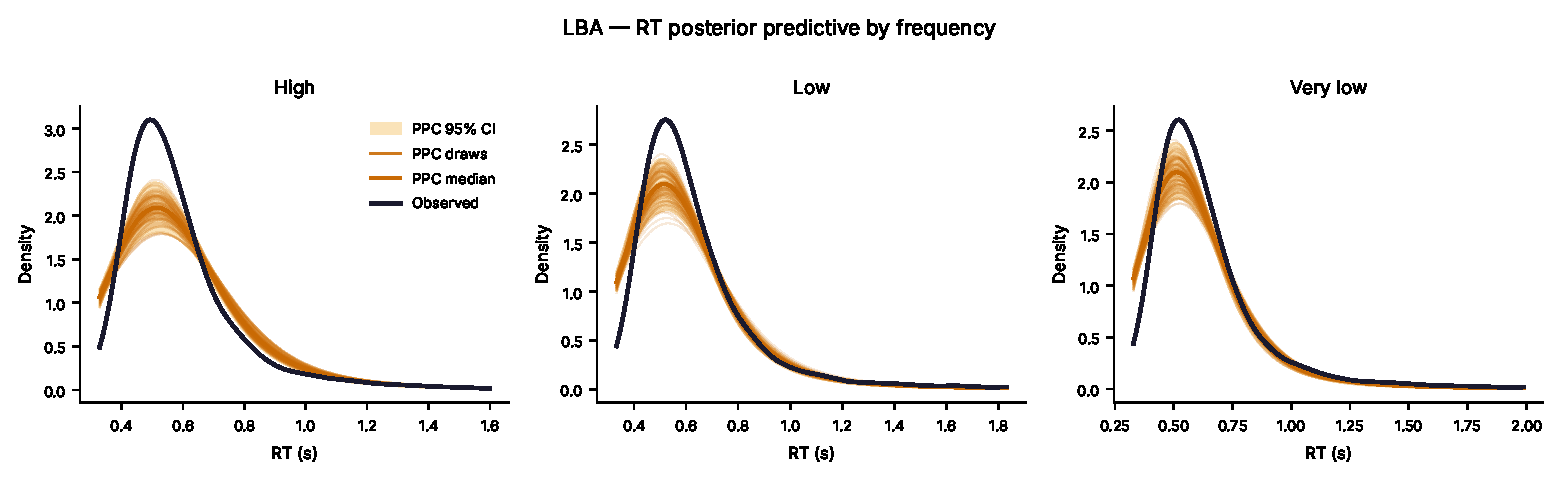
\includegraphics[width=\textwidth,height=0.18\textheight,keepaspectratio]{ppc/free/rt_ppc_frequency.pdf}
    \caption{RT densities}
  \end{subfigure}
  \caption{\textbf{LBA on empirical lexical-decision data: posterior predictive check by word frequency.} (a) RT quantiles and (b) RT densities, encoded as in Figure~\ref{fig:app3-realdata-condition}. Word frequency is not part of the fitted design, so the predictive distribution is identical across its levels by construction; differences between levels in the observed data are effects the fitted model does not represent.}
  \label{fig:app3-realdata-frequency}
\end{figure}

\begin{figure}[p]
  \centering
  \begin{subfigure}{\textwidth}\centering
    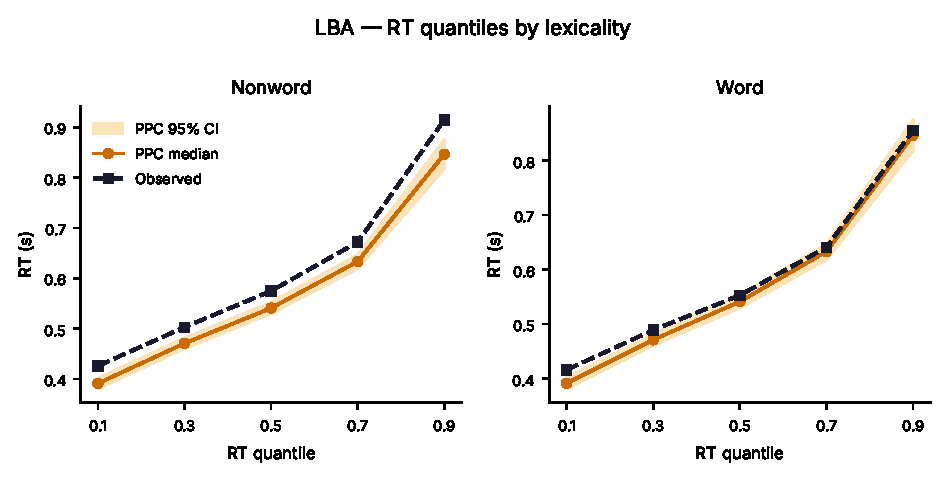
\includegraphics[width=\textwidth,height=0.18\textheight,keepaspectratio]{ppc/free/rt_quantiles_lexicality.pdf}
    \caption{RT quantiles}
  \end{subfigure}\\[0.5ex]
  \begin{subfigure}{\textwidth}\centering
    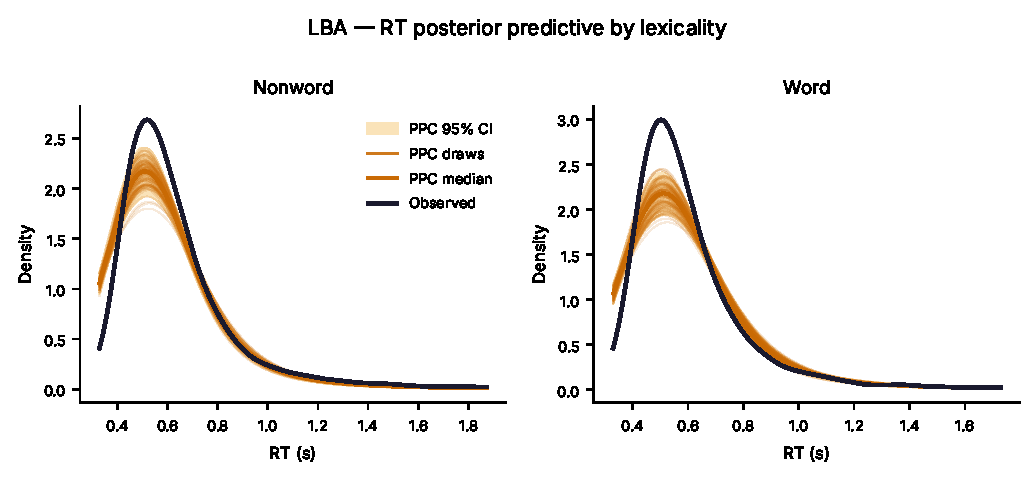
\includegraphics[width=\textwidth,height=0.18\textheight,keepaspectratio]{ppc/free/rt_ppc_lexicality.pdf}
    \caption{RT densities}
  \end{subfigure}
  \caption{\textbf{LBA on empirical lexical-decision data: posterior predictive check by lexicality.} (a) RT quantiles and (b) RT densities, encoded as in Figure~\ref{fig:app3-realdata-condition}. Lexicality enters only as the favoured accumulator, with the same drift advantage for words and nonwords; as a factor it is not part of the fitted design, so the predictive distribution is identical across its levels by construction; differences between levels in the observed data are effects the fitted model does not represent.}
  \label{fig:app3-realdata-lexicality}
\end{figure}
